% Options for packages loaded elsewhere
\PassOptionsToPackage{unicode}{hyperref}
\PassOptionsToPackage{hyphens}{url}
\PassOptionsToPackage{dvipsnames,svgnames,x11names}{xcolor}
%
\documentclass[
  10pt,
]{article}
\usepackage{amsmath,amssymb}
\usepackage{iftex}
\ifPDFTeX
  \usepackage[T1]{fontenc}
  \usepackage[utf8]{inputenc}
  \usepackage{textcomp} % provide euro and other symbols
\else % if luatex or xetex
  \usepackage{unicode-math} % this also loads fontspec
  \defaultfontfeatures{Scale=MatchLowercase}
  \defaultfontfeatures[\rmfamily]{Ligatures=TeX,Scale=1}
\fi
\usepackage{lmodern}
\ifPDFTeX\else
  % xetex/luatex font selection
\fi
% Use upquote if available, for straight quotes in verbatim environments
\IfFileExists{upquote.sty}{\usepackage{upquote}}{}
\IfFileExists{microtype.sty}{% use microtype if available
  \usepackage[]{microtype}
  \UseMicrotypeSet[protrusion]{basicmath} % disable protrusion for tt fonts
}{}
\makeatletter
\@ifundefined{KOMAClassName}{% if non-KOMA class
  \IfFileExists{parskip.sty}{%
    \usepackage{parskip}
  }{% else
    \setlength{\parindent}{0pt}
    \setlength{\parskip}{6pt plus 2pt minus 1pt}}
}{% if KOMA class
  \KOMAoptions{parskip=half}}
\makeatother
\usepackage{xcolor}
\usepackage{longtable,booktabs,array}
\usepackage{calc} % for calculating minipage widths
% Correct order of tables after \paragraph or \subparagraph
\usepackage{etoolbox}
\makeatletter
\patchcmd\longtable{\par}{\if@noskipsec\mbox{}\fi\par}{}{}
\makeatother
% Allow footnotes in longtable head/foot
\IfFileExists{footnotehyper.sty}{\usepackage{footnotehyper}}{\usepackage{footnote}}
\makesavenoteenv{longtable}
\usepackage{graphicx}
\makeatletter
\def\maxwidth{\ifdim\Gin@nat@width>\linewidth\linewidth\else\Gin@nat@width\fi}
\def\maxheight{\ifdim\Gin@nat@height>\textheight\textheight\else\Gin@nat@height\fi}
\makeatother
% Scale images if necessary, so that they will not overflow the page
% margins by default, and it is still possible to overwrite the defaults
% using explicit options in \includegraphics[width, height, ...]{}
\setkeys{Gin}{width=\maxwidth,height=\maxheight,keepaspectratio}
% Set default figure placement to htbp
\makeatletter
\def\fps@figure{htbp}
\makeatother
\setlength{\emergencystretch}{3em} % prevent overfull lines
\providecommand{\tightlist}{%
  \setlength{\itemsep}{0pt}\setlength{\parskip}{0pt}}
\setcounter{secnumdepth}{5}

\usepackage{amsmath,amssymb}
\usepackage{graphicx}
\usepackage{longtable,booktabs,array}
\usepackage{xcolor}
\usepackage[margin=2.1cm]{geometry}
\usepackage{microtype}
\setlength{\emergencystretch}{3em}
\pdfinfoomitdate=1
\pdftrailerid{}
\pdfsuppressptexinfo=-1
\renewcommand{\arraystretch}{1.15}
\allowdisplaybreaks
\ifLuaTeX
  \usepackage{selnolig}  % disable illegal ligatures
\fi
\IfFileExists{bookmark.sty}{\usepackage{bookmark}}{\usepackage{hyperref}}
\IfFileExists{xurl.sty}{\usepackage{xurl}}{} % add URL line breaks if available
\urlstyle{same}
\hypersetup{
  pdftitle={UM-2 analysis},
  pdfauthor={Underlying theory: Patrick L. Nash; Derived and verified by Claude (Anthropic); Analysis, version 4, 2026-10-18 (versions 1 to 3: 2026-10-17 and 2026-10-18); Repository once-ere/Dirac\_claude, folder universe\_model\_2},
  colorlinks=true,
  linkcolor={blue},
  filecolor={Maroon},
  citecolor={Blue},
  urlcolor={blue},
  pdfcreator={LaTeX via pandoc}}

\title{UM-2 analysis}
\usepackage{etoolbox}
\makeatletter
\providecommand{\subtitle}[1]{% add subtitle to \maketitle
  \apptocmd{\@title}{\par {\large #1 \par}}{}{}
}
\makeatother
\subtitle{The \(x_0\) mass mechanism, and the validity of associating
dark matter and dark energy with the dirac16complex field}
\author{Underlying theory: Patrick L. Nash \and Derived and verified by
Claude (Anthropic) \and Analysis, version 4, 2026-10-18 (versions 1 to
3: 2026-10-17 and 2026-10-18) \and Repository once-ere/Dirac\_claude,
folder universe\_model\_2}
\date{}

\begin{document}
\maketitle

{
\hypersetup{linkcolor=}
\setcounter{tocdepth}{3}
\tableofcontents
}
\hypertarget{how-to-read-this-document}{%
\section*{How to read this document}\label{how-to-read-this-document}}
\addcontentsline{toc}{section}{How to read this document}

\textbf{What it contains.} On 2026-10-18 the author ordered two analyses
of the universe model UM-2: ``analyze the \(x_0\) mass mechanism, and
\ldots{} analyze the validity of associating dark matter (and dark
energy) with dirac16complex''. This document carries out both. Part A
analyses the mechanism by which every non-massless particle receives its
mass from the dependence of its wave function on the hidden space
coordinate \(x_0\), periodic with the period \(\pi/(6H)\), with the
uncertainty relation as its physical reason; it states the author's
argument as equations, shows what it gives quantitatively and where it
fails, writes out the exact \(x_0\) eigenvalue equations of every field,
and explains the hierarchy of the masses, the mixing matrices and the
massless zero modes. Part B analyses dirac16complex as dark matter (the
candidate, the portals that produce it, its relic density from the
Boltzmann equation, its detection, the bound on its self-interaction and
the cosmological tests) and as dark energy (why this association is not
supported). The last two sections collect the conditions, the open
problems, the conflicts with data and the closing assessment.

\textbf{Version 4.} Version 4 (2026-10-18) re-presents version 3. The
physics and the numbers are those of version 3, taken from the current
outputs of the computations of the repository (after the precision fixes
of the commit of 2026-10-18 that added the residual analysis of the
solution: 287 checks in all), with the results of that residual analysis
where they concern this document. What is new is the presentation,
ordered by the author: every equation that is used is written out here,
every field equation and interaction term with the tag of the inventory
of the field equations of UM-2, (FE-\(n\)) or (IN-\(n\)), and every
display equation is followed by the list of all of its symbols with
their meanings, units, values and status. A symbol has one meaning
throughout (the notation of version 4: for example \(\tilde m^2\) is the
dimensionless boson eigenvalue, \(\tilde\varepsilon\) the dimensionless
fermion eigenvalue, \(K = 1/f^2\) the block variable, \(\mathcal{H}\)
the Hubble rate and \(H\) always the author's constant). The reader
never needs another document: every equation, definition and argument
used is in this one. The repository files that hold the computations are
named only for reproduction. Besides the re-presentation, two elementary
consequences of version-3 results are made explicit (the lower bound
that the uncertainty relation sets on a localised state, never below
11.05 TeV, and the asymptotic sensitivity of a zero-mode mass to its
localisation), the trace anomaly of the direct-detection estimate is
written in the geometric normalisation of the gluon field (the number is
unchanged), and the accuracy statements of the residual analysis are
added.

\textbf{Status labels.} AUTHOR (the author's notebooks and orders),
RECORD (the Revision record of this repository), STANDARD (textbook
physics or a measured value), ASSUMED (a choice made in UM-2), INVENTED
(a new interaction or structure of UM-2), DERIVED (computed and verified
in UM-2; the verification is stated), ESTIMATE (an order-of-magnitude
evaluation), OPEN (not solved). A measured bound that is quoted from
memory, not re-read from its source, is marked FROM MEMORY, as in
version 3.

\textbf{Units and conventions.} Natural units \(\hbar = c = 1\) (the
reduced Planck constant \(\hbar\) is shown where the author's relations
contain it). The coordinates are the author's
\(X = \{x_0, x_1, \dots, x_7\}\), the hidden direction first: \(x_0\)
the hidden space-like direction, \(x_1, x_2, x_3\) ordinary space,
\(x_4\) the time, \(x_5, x_6, x_7\) the three extra times. \(W^+\)
carries the electric charge \(+e\) and \(W^-\) the charge \(-e\). UM-2
contains no Higgs particle: the tip sigma field gives the \(W^\pm\) and
\(Z\) masses. A derivative with respect to \(\xi\) is always written
\(\mathrm{d}/\mathrm{d}\xi\), a dot is \(\mathrm{d}/\mathrm{d}x_4\), and
\(\Delta\) is a change, a difference or (in an uncertainty relation) the
root-mean-square spread of the quantity that follows.

\textbf{Where the numbers come from.} The scripts in the folder
\texttt{code} of \texttt{universe\_model\_2} write the outputs in the
folder \texttt{outputs}, with named checks in the folder
\texttt{reports}: \texttt{analysis.json} (the uncertainty analysis, the
sensitivities, the condensate), \texttt{masses.json},
\texttt{flavour.json} and \texttt{series.json} (the \(x_0\) spectra and
the Kaluza-Klein tower), \texttt{thermal.json} and \texttt{coupled.json}
(the thermal history, the relic, the portals, the coupled solution),
\texttt{neutrino.json} and \texttt{cosmology.json} (the neutrinos,
\(N_{\mathrm{eff}}\), the CMB) and \texttt{residuals.json} (the
residuals of the solution in every field equation and in concert).

\textbf{Summary of the verdicts.}

\begin{longtable}[]{@{}
  >{\raggedright\arraybackslash}p{(\columnwidth - 2\tabcolsep) * \real{0.1667}}
  >{\raggedright\arraybackslash}p{(\columnwidth - 2\tabcolsep) * \real{0.8333}}@{}}
\toprule\noalign{}
\begin{minipage}[b]{\linewidth}\raggedright
question
\end{minipage} & \begin{minipage}[b]{\linewidth}\raggedright
verdict
\end{minipage} \\
\midrule\noalign{}
\endhead
\bottomrule\noalign{}
\endlastfoot
Can every mass come from the \(x_0\) dependence of wave functions
periodic with period \(\pi/(6H)\)? & YES (DERIVED): every
four-dimensional mass of UM-2 (\(W^\pm\), \(Z\), the twelve fermions of
three generations, the dark matter, the Kaluza-Klein modes) is an
eigenvalue of an \(x_0\) operator; the graviton, the photon, the gluons
and the fold bands of dirac16complex are exactly massless \\
Is the uncertainty relation the reason for the masses? & ONLY FOR THE
HEAVY STATES: the uncertainty estimate \(m_{\mathrm{Heis}}\) lies below
the masses of the computed Kaluza-Klein and odd excitations and of the
dark matter (by factors 2.3 to 7.5), but the light masses (\(W^\pm\),
\(Z\) and all twelve fermions) lie \(3.2\times10^{-3}\) (top quark) to
\(1.1\times10^{-17}\) (lightest neutrino) below it and come from the tip
of the \(x_0\) cell \\
Why must the light fermions be zero modes? & The hidden kinetic energy
of any profile that is negligible at the tip is at least that of a mass
\(m_{\mathrm{Heis}} \ge 1/(2fL) = 11\) TeV (DERIVED); a mass of 173 GeV
or less needs an exact cancellation of it by the other terms of the
\(x_0\) operator, which happens only for the zero modes of that
operator; their mass is then the small mixing of two chiral zero modes
at the tip \\
Are the neutrino masses and their mixing \(x_0\) effects? & YES for the
masses, NO for the mixing angles: the three neutrino masses are \(x_0\)
eigenvalues (the most block-sensitive of all eigenvalues), the PMNS
matrix is the tip matrix \(\mathcal{K}_\nu\), an input; given both, the
flavour conversion follows \\
Do the extra times deflate to irrelevance? & IN THE PRIMORDIAL ERA, then
FROZEN: they deflate by up to a factor 2.9 into the stabilised block; a
continuing deflation is excluded because every mass and coupling depends
on the block size \\
Is dirac16complex dark matter? & YES, CONDITIONALLY: the lightest odd
quanta of its two halves \(\Psi_A\) and \(\Psi_B\) (two degenerate Dirac
fermions of 44.35 TeV) are cold, neutral and stable (DERIVED,
conditional); the gauge-kinetic portal I12 alone cannot produce their
relic abundance within perturbative unitarity, but with the s-wave
portal I13 (INVENTED) they freeze out with
\(\Omega_{\mathrm{DM}}h_{100}^2 = 0.060\) each (physics accuracy of the
needed coupling about 1 \%), and their scattering on xenon is 0.16 of
the present LZ limit (testable); the massless fold bands are radiation
(\(\Delta N_{\mathrm{eff}} = 0.001\) by freeze-in), not dark matter \\
Is dirac16complex dark energy? & NOT SUPPORTED: no positive-energy state
has a negative equation of state; a negative-coupling condensate runs
away; the dark energy of UM-2 is a tuned four-dimensional cosmological
term \\
Does the \(x_0\) mechanism fix the nucleon mass? & INDIRECTLY: the
nucleon mass is QCD binding energy, proportional to
\(\Lambda_{\mathrm{QCD}}\), which is set by the gauge coupling at the
Kaluza-Klein scale, itself an \(x_0\) quantity;
\(\mathrm{d}\ln m_{\mathrm{p}}/\mathrm{d}\ln f = -46.1\) makes it the
most block-sensitive mass of UM-2 \\
\end{longtable}

\hypertarget{a.-the-x_0-mass-mechanism}{%
\section*{\texorpdfstring{A. The \(x_0\) mass
mechanism}{A. The x\_0 mass mechanism}}\label{a.-the-x_0-mass-mechanism}}
\addcontentsline{toc}{section}{A. The \(x_0\) mass mechanism}

\hypertarget{a.1-the-periodic-hidden-coordinate-the-fold-and-the-tip}{%
\subsection*{A.1 The periodic hidden coordinate, the fold and the
tip}\label{a.1-the-periodic-hidden-coordinate-the-fold-and-the-tip}}
\addcontentsline{toc}{subsection}{A.1 The periodic hidden coordinate,
the fold and the tip}

The hidden coordinate enters the metric through the angle variable
\(z = 6Hx_0\). The order-0 metric of UM-2, the first term of the power
series of the metric, is in the author's coordinates (AUTHOR)

\[
\begin{aligned}
\bar g = \mathrm{diag}\Big(&\mathrm{e}^{-2a_4}b_4\cot^2z,\ \mathrm{e}^{2a_4},\ \mathrm{e}^{2a_4},\ 
 \mathrm{e}^{2a_4},\ -1,\\
&-\mathrm{e}^{-2a_4}b_4(\sin^2z)^{1/6},\ -\mathrm{e}^{-2a_4}b_4(\sin^2z)^{1/6},\ -\mathrm{e}^{-2a_4}b_4(
 \sin^2z)^{1/6}\Big),
 \qquad z = 6Hx_0
\end{aligned} \tag{FE-31}
\] \textbf{Symbols in (FE-31).}

\begin{itemize}
\tightlist
\item
  \(\bar g_{MN}\): The order-0 (background) metric of the power series:
  the corrected primordial metric in the author's coordinates,
  determined by the two functions \(a_4(x_4)\) and \(b_4(x_4)\);
  \(\lvert\bar g\rvert\) is the absolute value of its determinant. Unit:
  dimensionless. Status: AUTHOR.
\item
  \(\mathrm{diag}\): A diagonal matrix with the listed entries on its
  diagonal (in the order of the coordinates \(x_0, x_1, \dots, x_7\)
  when it is a tensor in eight dimensions). Status: STANDARD.
\item
  \(\mathrm{e}\): Euler's number, the base of the natural logarithm;
  \(\mathrm{e}^{X}\) is the exponential of \(X\). Unit: dimensionless.
  Value: 2.718281828. Status: STANDARD.
\item
  \(a_4\): The author's metric function of the time \(x_4\) that scales
  ordinary 3-space: the scale factor of cosmology is
  \(\mathrm{e}^{a_4}\). Unit: dimensionless. Status: AUTHOR.
\item
  \(b_4\): The author's metric function of the time \(x_4\) in the
  hidden and extra-time components, \(b_4 > 0\). Unit: dimensionless.
  Status: AUTHOR.
\item
  \(z\): The angle variable of the hidden direction, \(z = 6Hx_0\); one
  period of \(x_0\) is \(0 < z < \pi\). Unit: dimensionless. Status:
  AUTHOR.
\item
  \(H\): The author's constant (an inverse length) that fixes the period
  \(\pi/(6H)\) of \(x_0\), the Lovelock couplings, the cosmological
  constant \(\Lambda = -10H^2\) and the mass parameter \(m_\Psi = H\).
  Unit: GeV (1/length). Value: 14.296 TeV (from the fit of
  \(m_{\mathrm{W}}\) and \(\rho_{\mathrm{EW},0}\)). Status: AUTHOR.
\item
  \(x_0\): The hidden space-like coordinate (listed first); the metric
  depends on it through \(z = 6Hx_0\), periodically with the period
  \(\pi/(6H)\). Unit: length. Status: AUTHOR.
\end{itemize}

and in the chart \(y\), which measures the hidden direction in proper
units of the block, with the block scale \(f\) and the rates of the
background (DERIVED)

\[
\begin{aligned}
&y = \frac{\ln\lvert\sin z\rvert}{6H},\qquad \mathrm{d}y = \cot z\,\mathrm{d}x_0,\qquad \xi =
 \frac{y}{L}\in[-1, 0],\\
&\bar g_{MN}\,\mathrm{d}X^M\mathrm{d}X^N = \mathrm{e}^{2a_4}\big(\mathrm{d}x_1^2 + \mathrm{d}x_2^2 +
 \mathrm{d}x_3^2\big)
 - \mathrm{d}x_4^2 + f^2\Big[\mathrm{d}y^2 - \mathrm{e}^{2Hy}\big(\mathrm{d}x_5^2 + \mathrm{d}x_6^2 +
 \mathrm{d}x_7^2\big)\Big],\\
&f = \mathrm{e}^{-a_4}b_4^{1/2},\qquad K = \frac{1}{f^2},\qquad \mathcal{H} = \dot a_4,\qquad
 \mathcal{H}_f = \frac{\dot f}{f} = \frac{\dot b_4}{2b_4} - \dot a_4,\qquad \dot K = -2K\mathcal{H}_f,\\
&\sqrt{\lvert\bar g\rvert} = \mathrm{e}^{3a_4}f^4\lvert\cot z\rvert(\sin^2z)^{1/4}
 = \mathrm{e}^{3a_4}f^4\,\mathrm{e}^{3Hy}\Big\lvert\frac{\mathrm{d}y}{\mathrm{d}x_0}\Big\rvert
\end{aligned} \tag{FE-32}
\] \textbf{Symbols in (FE-32).}

\begin{itemize}
\tightlist
\item
  \(y\): The hidden coordinate of the \(y\) chart,
  \(y = \ln\lvert\sin z\rvert/(6H)\), with \(y = 0\) at the fold
  (\(z = \pi/2\)) and \(y = -L\) at the regular tip; each half of a
  period of \(x_0\) is the interval \(-L \le y \le 0\). Unit: length.
  Status: DERIVED.
\item
  \(z\): The angle variable of the hidden direction, \(z = 6Hx_0\); one
  period of \(x_0\) is \(0 < z < \pi\). Unit: dimensionless. Status:
  AUTHOR.
\item
  \(H\): The author's constant (an inverse length) that fixes the period
  \(\pi/(6H)\) of \(x_0\), the Lovelock couplings, the cosmological
  constant \(\Lambda = -10H^2\) and the mass parameter \(m_\Psi = H\).
  Unit: GeV (1/length). Value: 14.296 TeV (from the fit of
  \(m_{\mathrm{W}}\) and \(\rho_{\mathrm{EW},0}\)). Status: AUTHOR.
\item
  \(\mathrm{d}\): The differential: \(\mathrm{d}X\) is an infinitesimal
  change of \(X\), \(\mathrm{d}X/\mathrm{d}Y\) the derivative of \(X\)
  with respect to \(Y\), \(\mathrm{d}^nX\) the volume element of \(n\)
  variables. Status: STANDARD.
\item
  \(x_0\): The hidden space-like coordinate (listed first); the metric
  depends on it through \(z = 6Hx_0\), periodically with the period
  \(\pi/(6H)\). Unit: length. Status: AUTHOR.
\item
  \(\xi\): The scaled hidden coordinate, \(\xi = y/L\), running from
  \(-1\) (tip) to \(0\) (fold) on each half of a period. Unit:
  dimensionless. Status: DERIVED.
\item
  \(L\): The depth of the regular tip: each half of a period of \(x_0\)
  ends at \(y = -L\); \(HL = 3\). Unit: length. Value: \(L = 3/H\)
  (\(fL = 8.926\times10^{-21}\) m at the stabilised block). Status:
  ASSUMED.
\item
  \(\bar g_{MN}\): The order-0 (background) metric of the power series:
  the corrected primordial metric in the author's coordinates,
  determined by the two functions \(a_4(x_4)\) and \(b_4(x_4)\);
  \(\lvert\bar g\rvert\) is the absolute value of its determinant. Unit:
  dimensionless. Status: AUTHOR.
\item
  \(M\): A coordinate index of eight dimensions (also with a numbered
  copy \(M_1, M_2, \dots\)): it runs over \(x_0, x_1, \dots, x_7\); a
  repeated index is summed. Status: STANDARD.
\item
  \(N\): A coordinate index of eight dimensions (also
  \(N_1, N_2, \dots\)), running over \(x_0, \dots, x_7\); a repeated
  index is summed. Status: STANDARD.
\item
  \(X = \{x_0, \dots, x_7\}\): The author's coordinates of the
  eight-dimensional spacetime, \(X = \{x_0, x_1, \dots, x_7\}\) with the
  hidden direction first; \(X^M\) is the coordinate with the index
  \(M\),
  \(\mathrm{d}^8X = \mathrm{d}x_0\,\mathrm{d}x_1\cdots\mathrm{d}x_7\)
  the coordinate volume element and \(X^\mu\) (four-dimensional index
  \(\mu\)) the observable coordinates \(x_1, \dots, x_4\). Unit: length
  (each coordinate). Status: AUTHOR.
\item
  \(\mathrm{e}\): Euler's number, the base of the natural logarithm;
  \(\mathrm{e}^{X}\) is the exponential of \(X\). Unit: dimensionless.
  Value: 2.718281828. Status: STANDARD.
\item
  \(a_4\): The author's metric function of the time \(x_4\) that scales
  ordinary 3-space: the scale factor of cosmology is
  \(\mathrm{e}^{a_4}\). Unit: dimensionless. Status: AUTHOR.
\item
  \(x_1\): The first coordinate of ordinary 3-space. Unit: length.
  Status: AUTHOR.
\item
  \(x_2\): The second coordinate of ordinary 3-space. Unit: length.
  Status: AUTHOR.
\item
  \(x_3\): The third coordinate of ordinary 3-space (also the symmetry
  axis of the fast-flavour analysis). Unit: length. Status: AUTHOR.
\item
  \(x_4\): The time; dots denote \(\mathrm{d}/\mathrm{d}x_4\). Unit:
  length (= time, c = 1). Status: AUTHOR.
\item
  \(f\): The block scale: the common scale factor of the hidden
  direction and the extra times, \(f = \mathrm{e}^{-a_4}b_4^{1/2}\) (the
  block is \(f^2\) times a four-dimensional space of constant curvature
  \(-H^2\)). Unit: dimensionless. Status: DERIVED.
\item
  \(x_5\): The first of the three extra time-like coordinates. Unit:
  length. Status: AUTHOR.
\item
  \(x_6\): The second of the three extra time-like coordinates. Unit:
  length. Status: AUTHOR.
\item
  \(x_7\): The third of the three extra time-like coordinates. Unit:
  length. Status: AUTHOR.
\item
  \(b_4\): The author's metric function of the time \(x_4\) in the
  hidden and extra-time components, \(b_4 > 0\). Unit: dimensionless.
  Status: AUTHOR.
\item
  \(K\): The block variable, \(K = 1/f^2\). Unit: dimensionless. Status:
  DERIVED.
\item
  \(\mathcal{H}\): The expansion rate of ordinary 3-space,
  \(\mathcal{H} = \dot a_4\) (the Hubble rate of the observer; in the
  hot Universe
  \(\mathcal{H} = (8\pi^3g_\rho/90)^{1/2}T^2/M_{\mathrm{Pl}}\)). Unit:
  GeV. Status: DERIVED.
\item
  \(\dot a_4\): The time derivative \(\mathrm{d}a_4/\mathrm{d}x_4\).
  Unit: GeV. Status: DERIVED.
\item
  \(\mathcal{H}_f\): The expansion rate of the block,
  \(\mathcal{H}_f = \dot f/f = \dot b_4/(2b_4) - \dot a_4\) (negative
  when the extra times and \(x_0\) deflate). Unit: GeV. Status: DERIVED.
\item
  \(\dot f\): The time derivative \(\mathrm{d}f/\mathrm{d}x_4\) of the
  block scale. Unit: GeV. Status: DERIVED.
\item
  \(\dot b_4\): The time derivative \(\mathrm{d}b_4/\mathrm{d}x_4\).
  Unit: GeV. Status: DERIVED.
\item
  \(\dot K\): The time derivative \(\mathrm{d}K/\mathrm{d}x_4\). Unit:
  GeV. Status: DERIVED.
\end{itemize}

One period \(0 < z < \pi\) of \(x_0\), of coordinate length
\(\pi/(6H) = 3.663\times10^{-5}\) GeV\(^{-1}\) \(= 7.23\times10^{-21}\)
m, consists of two halves joined at the fold \(y = 0\) (\(z = \pi/2\));
each half ends at a tip (\(y \to -\infty\)), which UM-2 replaces by a
regular cutoff at \(y = -L\) with \(HL = 3\) (ASSUMED). Every function
of \(y(z)\) is periodic in \(x_0\) with the period \(\pi/(6H)\), and so
is every wave function of UM-2: the author's periodicity requirement is
built into the geometry. On the stabilised block,
\(f = f_* = 0.215556\), the proper depth of one half is
\(fL = 8.926\times10^{-21}\) m, i.e. \(1/(fL) = 22.11\) TeV (DERIVED).

\hypertarget{a.2-the-authors-argument-in-equations}{%
\subsection*{A.2 The author's argument in
equations}\label{a.2-the-authors-argument-in-equations}}
\addcontentsline{toc}{subsection}{A.2 The author's argument in
equations}

The author's order of 2026-10-18 gives the reason for the masses in
three steps (AUTHOR). First, a particle whose wave function is localised
with respect to \(x_0\) obeys the uncertainty relation for the
coordinate \(x_0\) and the component \(k_{x_0}\) of its momentum along
\(x_0\) (with \(\hbar = 1\) the momentum and the wave number coincide):

\[ \Delta x_0\,\Delta k_{x_0} \ge \frac{\hbar}{2} \] \textbf{Symbols in
this equation.}

\begin{itemize}
\tightlist
\item
  \(\Delta\): The change (difference or small perturbation) of the
  quantity that follows: \(\Delta K\), \(\Delta\rho\), \(\Delta p_3\)
  are first-order changes about the static block,
  \(\Delta\varepsilon_o\) a level shift,
  \(\Delta m^2_{21} = m_2^2 - m_1^2\) a difference of squared masses,
  \(\Delta N_{\mathrm{eff}}\) an addition to \(N_{\mathrm{eff}}\),
  \(\Delta S_{\mathrm{m}}\) the change of an action under a change
  \(\Delta g^{MN}\) of the metric. Status: STANDARD.
\item
  \(x_0\): The hidden space-like coordinate (listed first); the metric
  depends on it through \(z = 6Hx_0\), periodically with the period
  \(\pi/(6H)\). Unit: length. Status: AUTHOR.
\item
  \(k_{x_0}\): The component of the momentum along the hidden coordinate
  \(x_0\), the momentum conjugate to \(x_0\) (the
  author\textquotesingle s \((p)_{x_0}\)); since \(\hbar = 1\) it is
  also the wave number of the \(x_0\) dependence. Unit: GeV. Status:
  AUTHOR.
\item
  \(\hbar\): The reduced Planck constant, which sets the scale of the
  uncertainty relation; it equals 1 in the natural units of this
  document, and \(\hbar c = 1.973269804\times10^{-16}\) GeV m converts
  an inverse mass into a length. Unit: GeV s (equal to 1 in natural
  units). Value: 1 (natural units). Status: STANDARD.
\end{itemize}

Second, the momentum may be thought of as proportional to the mass, and
the kinetic energy as proportional to the momentum squared divided by
the mass:

\[ k_{x_0} \propto m_{\mathrm{eff}},\qquad E_{\mathrm{kin}} \propto \frac{k_{x_0}^2}{m_{\mathrm{eff}}} \]
\textbf{Symbols in this equation.}

\begin{itemize}
\tightlist
\item
  \(k_{x_0}\): The component of the momentum along the hidden coordinate
  \(x_0\), the momentum conjugate to \(x_0\) (the
  author\textquotesingle s \((p)_{x_0}\)); since \(\hbar = 1\) it is
  also the wave number of the \(x_0\) dependence. Unit: GeV. Status:
  AUTHOR.
\item
  \(m_{\mathrm{eff}}\): The effective mass of the
  author\textquotesingle s argument: the mass that a particle receives
  from the \(x_0\) dependence of its wave function, estimated by taking
  the momentum \(k_{x_0}\) proportional to the mass and the kinetic
  energy proportional to the momentum squared over the mass. Unit: GeV.
  Status: AUTHOR.
\item
  \(E_{\mathrm{kin}}\): The kinetic energy of the motion along \(x_0\)
  in the author\textquotesingle s argument, proportional to
  \(k_{x_0}^2/m_{\mathrm{eff}}\). Unit: GeV. Status: AUTHOR.
\end{itemize}

Third, hence every particle whose wave function depends on \(x_0\),
periodically with the period \(\pi/(6H)\), has an effective mass, of the
order of the momentum spread that its localisation forces (up to factors
of order one, in natural units):

\[ m_{\mathrm{eff}} \sim \Delta k_{x_0} \ge \frac{\hbar}{2\Delta x_0} \]
\textbf{Symbols in this equation.}

\begin{itemize}
\tightlist
\item
  \(m_{\mathrm{eff}}\): The effective mass of the
  author\textquotesingle s argument: the mass that a particle receives
  from the \(x_0\) dependence of its wave function, estimated by taking
  the momentum \(k_{x_0}\) proportional to the mass and the kinetic
  energy proportional to the momentum squared over the mass. Unit: GeV.
  Status: AUTHOR.
\item
  \(\Delta\): The change (difference or small perturbation) of the
  quantity that follows: \(\Delta K\), \(\Delta\rho\), \(\Delta p_3\)
  are first-order changes about the static block,
  \(\Delta\varepsilon_o\) a level shift,
  \(\Delta m^2_{21} = m_2^2 - m_1^2\) a difference of squared masses,
  \(\Delta N_{\mathrm{eff}}\) an addition to \(N_{\mathrm{eff}}\),
  \(\Delta S_{\mathrm{m}}\) the change of an action under a change
  \(\Delta g^{MN}\) of the metric. Status: STANDARD.
\item
  \(k_{x_0}\): The component of the momentum along the hidden coordinate
  \(x_0\), the momentum conjugate to \(x_0\) (the
  author\textquotesingle s \((p)_{x_0}\)); since \(\hbar = 1\) it is
  also the wave number of the \(x_0\) dependence. Unit: GeV. Status:
  AUTHOR.
\item
  \(\hbar\): The reduced Planck constant, which sets the scale of the
  uncertainty relation; it equals 1 in the natural units of this
  document, and \(\hbar c = 1.973269804\times10^{-16}\) GeV m converts
  an inverse mass into a length. Unit: GeV s (equal to 1 in natural
  units). Value: 1 (natural units). Status: STANDARD.
\item
  \(x_0\): The hidden space-like coordinate (listed first); the metric
  depends on it through \(z = 6Hx_0\), periodically with the period
  \(\pi/(6H)\). Unit: length. Status: AUTHOR.
\end{itemize}

This holds, the author states, for all particles except the graviton,
the photon and perhaps the quanta of dirac16complex. The coordinate
\(x_0\) is not a proper length (its proper element
\(f\cot z\,\mathrm{d}x_0\) vanishes at the fold and diverges at the
tips; section A.6), so version 3 applied the argument to the proper
hidden length \(fy\), the proper distance from the fold, and defined the
author's estimate of the mass of a state as (DERIVED from the AUTHOR
argument)

\[ m_{\mathrm{Heis}} = \frac{\hbar}{2\Delta(fy)},\qquad \Delta(fy) = fL\,\Delta\xi,\qquad \Delta\xi^2 = \int_{-1}^{0}\xi^2\varrho_\xi\,\mathrm{d}\xi \]
\textbf{Symbols in this equation.}

\begin{itemize}
\tightlist
\item
  \(m_{\mathrm{Heis}}\): The author\textquotesingle s uncertainty
  (Heisenberg) estimate of the mass of a state,
  \(m_{\mathrm{Heis}} = \hbar/(2\Delta(fy))\), where
  \(\Delta(fy) = fL\,\Delta\xi\) is the root-mean-square proper distance
  of the state from the fold
  (\(\Delta\xi^2 = \int_{-1}^{0}\xi^2\varrho_\xi\,\mathrm{d}\xi\)). It
  is the lower bound on the mass that the uncertainty relation would
  give if the hidden kinetic energy were the whole mass and the state
  were negligible at the tip. (The subscript stands for Heisenberg; UM-2
  has no Higgs particle.) Unit: GeV. Value: 70.56 TeV (photon, gluons,
  graviton, \(W^\pm\), \(Z\)); 53.80 TeV (quark-doublet zero mode);
  93.08 TeV (lepton-doublet zero mode); 22.90 TeV (fold band of
  dirac16complex); 19.39 TeV (dark matter); at least \(1/(2fL) = 11.05\)
  TeV for every profile on the cell. Status: DERIVED.
\item
  \(\hbar\): The reduced Planck constant, which sets the scale of the
  uncertainty relation; it equals 1 in the natural units of this
  document, and \(\hbar c = 1.973269804\times10^{-16}\) GeV m converts
  an inverse mass into a length. Unit: GeV s (equal to 1 in natural
  units). Value: 1 (natural units). Status: STANDARD.
\item
  \(\Delta\): The change (difference or small perturbation) of the
  quantity that follows: \(\Delta K\), \(\Delta\rho\), \(\Delta p_3\)
  are first-order changes about the static block,
  \(\Delta\varepsilon_o\) a level shift,
  \(\Delta m^2_{21} = m_2^2 - m_1^2\) a difference of squared masses,
  \(\Delta N_{\mathrm{eff}}\) an addition to \(N_{\mathrm{eff}}\),
  \(\Delta S_{\mathrm{m}}\) the change of an action under a change
  \(\Delta g^{MN}\) of the metric. Status: STANDARD.
\item
  \(f\): The block scale: the common scale factor of the hidden
  direction and the extra times, \(f = \mathrm{e}^{-a_4}b_4^{1/2}\) (the
  block is \(f^2\) times a four-dimensional space of constant curvature
  \(-H^2\)). Unit: dimensionless. Status: DERIVED.
\item
  \(y\): The hidden coordinate of the \(y\) chart,
  \(y = \ln\lvert\sin z\rvert/(6H)\), with \(y = 0\) at the fold
  (\(z = \pi/2\)) and \(y = -L\) at the regular tip; each half of a
  period of \(x_0\) is the interval \(-L \le y \le 0\). Unit: length.
  Status: DERIVED.
\item
  \(L\): The depth of the regular tip: each half of a period of \(x_0\)
  ends at \(y = -L\); \(HL = 3\). Unit: length. Value: \(L = 3/H\)
  (\(fL = 8.926\times10^{-21}\) m at the stabilised block). Status:
  ASSUMED.
\item
  \(\xi\): The scaled hidden coordinate, \(\xi = y/L\), running from
  \(-1\) (tip) to \(0\) (fold) on each half of a period. Unit:
  dimensionless. Status: DERIVED.
\item
  \(\varrho_\xi\): The probability density in \(\xi\) of the \(x_0\)
  profile of a mode on one half of the period, normalised as
  \(\int_{-1}^{0}\varrho_\xi\,\mathrm{d}\xi = 1\):
  \(\varrho_\xi = \tilde F^2/\int_{-1}^{0}\tilde F^2\mathrm{d}\xi\) for
  a boson (\(\tilde F = \mathrm{e}^{3HL\xi/2}F\), the flat measure) and
  \(\varrho_\xi = \chi^\dagger\chi/\int_{-1}^{0}\chi^\dagger\chi\,\mathrm{d}\xi\)
  for a fermion. \(\varrho_\xi(0)\) is its value at the fold,
  \(\varrho_\xi(-1)\) its value at the tip; over the full period the
  density is symmetric about the fold. Unit: dimensionless. Status:
  DERIVED.
\item
  \(\mathrm{d}\): The differential: \(\mathrm{d}X\) is an infinitesimal
  change of \(X\), \(\mathrm{d}X/\mathrm{d}Y\) the derivative of \(X\)
  with respect to \(Y\), \(\mathrm{d}^nX\) the volume element of \(n\)
  variables. Status: STANDARD.
\end{itemize}

where \(\Delta(fy)\) is the root-mean-square proper distance from the
fold and \(\varrho_\xi\) the probability density of the state in \(\xi\)
on one half of the period, in the measure in which the hidden kinetic
energy is a plain \(\int(\mathrm{d}/\mathrm{d}\xi)^2\):

\[ \varrho_\xi = \frac{\tilde F^2}{\int_{-1}^{0}\tilde F^2\,\mathrm{d}\xi}\ \ (\text{boson},\ F = \mathrm{e}^{-3HL\xi/2}\tilde F),\qquad \varrho_\xi = \frac{\chi^\dagger\chi}{\int_{-1}^{0}\chi^\dagger\chi\,\mathrm{d}\xi}\ \ (\text{fermion}) \]
\textbf{Symbols in this equation.}

\begin{itemize}
\tightlist
\item
  \(\varrho_\xi\): The probability density in \(\xi\) of the \(x_0\)
  profile of a mode on one half of the period, normalised as
  \(\int_{-1}^{0}\varrho_\xi\,\mathrm{d}\xi = 1\):
  \(\varrho_\xi = \tilde F^2/\int_{-1}^{0}\tilde F^2\mathrm{d}\xi\) for
  a boson (\(\tilde F = \mathrm{e}^{3HL\xi/2}F\), the flat measure) and
  \(\varrho_\xi = \chi^\dagger\chi/\int_{-1}^{0}\chi^\dagger\chi\,\mathrm{d}\xi\)
  for a fermion. \(\varrho_\xi(0)\) is its value at the fold,
  \(\varrho_\xi(-1)\) its value at the tip; over the full period the
  density is symmetric about the fold. Unit: dimensionless. Status:
  DERIVED.
\item
  \(\tilde F\): The rescaled boson profile,
  \(F = \mathrm{e}^{-3HL\xi/2}\tilde F\). Unit: dimensionless. Status:
  DERIVED.
\item
  \(\mathrm{d}\): The differential: \(\mathrm{d}X\) is an infinitesimal
  change of \(X\), \(\mathrm{d}X/\mathrm{d}Y\) the derivative of \(X\)
  with respect to \(Y\), \(\mathrm{d}^nX\) the volume element of \(n\)
  variables. Status: STANDARD.
\item
  \(\xi\): The scaled hidden coordinate, \(\xi = y/L\), running from
  \(-1\) (tip) to \(0\) (fold) on each half of a period. Unit:
  dimensionless. Status: DERIVED.
\item
  \(F(\xi),\ F_n\): The \(x_0\) profile of a boson mode on one half of
  the period (a function of \(y\) or of \(\xi = y/L\)): of a gauge field
  (gauge \(A_y = 0\)) or of the transverse-traceless graviton; \(F_n\)
  is the profile of the \(n\)-th Kaluza-Klein level of the graviton
  tower (\(F_0 = 1\) the flat zero mode). Unit: dimensionless. Status:
  DERIVED.
\item
  \(\mathrm{e}\): Euler's number, the base of the natural logarithm;
  \(\mathrm{e}^{X}\) is the exponential of \(X\). Unit: dimensionless.
  Value: 2.718281828. Status: STANDARD.
\item
  \(H\): The author's constant (an inverse length) that fixes the period
  \(\pi/(6H)\) of \(x_0\), the Lovelock couplings, the cosmological
  constant \(\Lambda = -10H^2\) and the mass parameter \(m_\Psi = H\).
  Unit: GeV (1/length). Value: 14.296 TeV (from the fit of
  \(m_{\mathrm{W}}\) and \(\rho_{\mathrm{EW},0}\)). Status: AUTHOR.
\item
  \(L\): The depth of the regular tip: each half of a period of \(x_0\)
  ends at \(y = -L\); \(HL = 3\). Unit: length. Value: \(L = 3/H\)
  (\(fL = 8.926\times10^{-21}\) m at the stabilised block). Status:
  ASSUMED.
\item
  \(\chi,\ \chi_o,\ \chi_1,\ \chi_2\): The two-component spinor of one
  block of the reduction (a function of \(y\) and \(x_4\)),
  \(\chi = (\chi_1, \chi_2)^T = (a, \mathrm{i}b)^T\); \(\chi_o\) the
  Kohn-Sham orbital \(o\), normalised as
  \(\int_{-L}^{0}\chi_o^\dagger\chi_o\,\mathrm{d}y = 1\). Unit:
  \(\mathrm{GeV}^{1/2}\) (normalised orbital). Status: DERIVED.
\item
  \({}^\dagger\): Hermitian conjugation: the complex conjugate of the
  transpose of a matrix or spinor (for field operators the adjoint
  operator). Status: STANDARD.
\end{itemize}

Over the full period the density is symmetric about the fold, so
\(\Delta\xi\) is also the spread of the full-period profile. The
argument is a heuristic. UM-2 tests it in two steps: every mass is
computed exactly as an eigenvalue of the \(x_0\) operator of its field
(section A.3), and each eigenvalue is split exactly into the hidden
kinetic energy, which the uncertainty relation bounds, and the remaining
terms of the operator, which it does not (section A.4).

\hypertarget{a.3-every-mass-is-an-x_0-eigenvalue-the-exact-equations}{%
\subsection*{\texorpdfstring{A.3 Every mass is an \(x_0\) eigenvalue:
the exact
equations}{A.3 Every mass is an x\_0 eigenvalue: the exact equations}}\label{a.3-every-mass-is-an-x_0-eigenvalue-the-exact-equations}}
\addcontentsline{toc}{subsection}{A.3 Every mass is an \(x_0\)
eigenvalue: the exact equations}

\hypertarget{the-tip-of-the-cell-electroweak-symmetry-breaking-without-a-higgs-particle-invented}{%
\subsubsection*{The tip of the cell: electroweak symmetry breaking
without a Higgs particle
(INVENTED)}\label{the-tip-of-the-cell-electroweak-symmetry-breaking-without-a-higgs-particle-invented}}
\addcontentsline{toc}{subsubsection}{The tip of the cell: electroweak
symmetry breaking without a Higgs particle (INVENTED)}

The masses of \(W^\pm\), \(Z\) and of all fermions originate at the
regular tip \(y = -L\) of the cell, where a non-linear sigma field
carries the electroweak symmetry breaking and couples the doublet zero
modes to the singlet zero modes:

\[
\begin{aligned}
S_{\mathrm{tip}} &= \int_{y=-L}\mathrm{d}^7X_{\mathrm{tip}}\sqrt{\lvert g_{\mathrm{tip}}\rvert}\,\Big[
 -\frac{v_\Sigma^2}{4}\,\mathrm{tr}\big((D_\mu\Sigma)^\dagger D^\mu\Sigma\big) -
 \mathcal{L}_{\mathrm{Y}}\Big],\\
\mathcal{L}_{\mathrm{Y}} &=
 \sum_{i,j=1}^{3}\Big[\bar\ell_i\,\Sigma\begin{pmatrix}(\mathcal{Y}_\nu)_{ij}\,\nu_{Rj}\\
 (\mathcal{Y}_e)_{ij}\,e_{Rj}\end{pmatrix}
 + \bar Q_i\,\Sigma\begin{pmatrix}(\mathcal{Y}_u)_{ij}\,u_{Rj}\\ (\mathcal{Y}_d)_{ij}\,d_{Rj}
 \end{pmatrix}\Big]
 + \text{h.c.}
\end{aligned} \tag{IN-13}
\] \textbf{Symbols in (IN-13).}

\begin{itemize}
\tightlist
\item
  \(S_{\mathrm{tip}}\): The action on the tip \(y = -L\): the sigma
  field and the tip Yukawa couplings. Unit: dimensionless. Status:
  INVENTED.
\item
  \(y\): The hidden coordinate of the \(y\) chart,
  \(y = \ln\lvert\sin z\rvert/(6H)\), with \(y = 0\) at the fold
  (\(z = \pi/2\)) and \(y = -L\) at the regular tip; each half of a
  period of \(x_0\) is the interval \(-L \le y \le 0\). Unit: length.
  Status: DERIVED.
\item
  \(L\): The depth of the regular tip: each half of a period of \(x_0\)
  ends at \(y = -L\); \(HL = 3\). Unit: length. Value: \(L = 3/H\)
  (\(fL = 8.926\times10^{-21}\) m at the stabilised block). Status:
  ASSUMED.
\item
  \(\mathrm{d}\): The differential: \(\mathrm{d}X\) is an infinitesimal
  change of \(X\), \(\mathrm{d}X/\mathrm{d}Y\) the derivative of \(X\)
  with respect to \(Y\), \(\mathrm{d}^nX\) the volume element of \(n\)
  variables. Status: STANDARD.
\item
  \(X_{\mathrm{tip}}\): The seven coordinates \(x_1, \dots, x_7\) of the
  tip \(y = -L\) of the hidden direction;
  \(\mathrm{d}^7X_{\mathrm{tip}}\) is their coordinate volume element.
  Unit: length (each coordinate). Status: DERIVED.
\item
  \(g_{\mathrm{tip}}\): The metric induced on the seven-dimensional tip
  \(y = -L\) (the metric \(g_{MN}\) restricted to the tip directions
  \(x_1, \dots, x_7\)); \(\lvert g_{\mathrm{tip}}\rvert\) is the
  absolute value of its determinant. Unit: dimensionless. Status:
  DERIVED.
\item
  \(v_\Sigma\): The scale of the tip sigma field (its kinetic term is
  \(-\frac{v_\Sigma^2}{4}\mathrm{tr}((D_\mu\Sigma)^\dagger D^\mu\Sigma)\));
  on the static block it fixes the Robin parameter
  \(\beta_{\mathrm{W}}\). Unit: \(\mathrm{GeV}^{5/2}\). Value: fixed
  through \(\beta_{\mathrm{W}} = 0.011912\). Status: INVENTED.
\item
  \(\mathrm{tr}\): The trace of a matrix: the sum of its diagonal
  entries. Status: STANDARD.
\item
  \(D_M,\ D_\mu\): The covariant derivative: on a spinor
  \(D_M = \partial_M + \Omega_M\) (spin connection), on a Standard-Model
  fermion with the gauge fields added; on the sigma field
  \(D_\mu\Sigma\) with the \(W\) and \(B\) fields. Unit: 1/length.
  Status: STANDARD.
\item
  \(\mu\): A four-dimensional coordinate index running over the
  observable coordinates \(x_1, x_2, x_3, x_4\) (signature \(+,+,+,-\));
  on the tip it runs over the tip directions; a repeated index is
  summed. Status: STANDARD.
\item
  \(\Sigma\): The tip sigma field: a unitary \(2 \times 2\) matrix field
  on the tip (\(\Sigma^\dagger\Sigma = \mathbf{1}\)) that replaces the
  Higgs doublet; its three modes are the longitudinal \(W^+\), \(W^-\)
  and \(Z\), and \(\Sigma = \mathbf{1}\) is the unitary gauge. Unit:
  dimensionless. Status: INVENTED.
\item
  \({}^\dagger\): Hermitian conjugation: the complex conjugate of the
  transpose of a matrix or spinor (for field operators the adjoint
  operator). Status: STANDARD.
\item
  \(\mathcal{L}_{\mathrm{Y}}\): The tip Yukawa Lagrangian: the couplings
  of the doublets to the singlets through the sigma field and the tip
  matrices \(\mathcal{Y}\) (plus the Hermitian conjugate, h.c.). Unit:
  \(\mathrm{GeV}^{7}\). Status: INVENTED.
\item
  \(i\): The generation index (\(i = 1, 2, 3\)), which also labels the
  neutrino mass states \(\nu_1, \nu_2, \nu_3\); a repeated index is not
  summed unless a sum sign is written. Status: STANDARD.
\item
  \(j\): A second generation index (\(j = 1, 2, 3\)). Status: STANDARD.
\item
  \(\ell_i,\ \bar\ell_i\): The lepton doublet of the generation \(i\)
  (left-handed neutrino and charged lepton) and its Dirac adjoint. Unit:
  \(\mathrm{GeV}^{7/2}\). Status: ASSUMED.
\item
  \(\mathcal{Y}_\nu,\ \mathcal{Y}_e,\ \mathcal{Y}_u,\ \mathcal{Y}_d\):
  The complex \(3 \times 3\) tip Yukawa matrices of the neutrino,
  charged-lepton, up-quark and down-quark sectors (generation indices
  \(i, j\)); on the static block they become the tip mixing matrices
  \(\mathcal{K}\) (the normalisation of that relation is not fixed:
  OPEN). Unit: dimensionless. Status: INVENTED.
\item
  \(\nu_R,\ \nu_{Ri}\): The right-handed neutrino (a gauge singlet):
  \(\nu_R\) the multiplet, \(\nu_{Ri}\) that of the generation \(i\);
  its zero modes give Dirac neutrino masses. Unit:
  \(\mathrm{GeV}^{7/2}\). Status: ASSUMED.
\item
  \(e_R,\ e_{Ri}\): The right-handed charged-lepton singlet: \(e_R\) the
  multiplet, \(e_{Ri}\) that of the generation \(i\) (\(e_R\),
  \(\mu_R\), \(\tau_R\)). Unit: \(\mathrm{GeV}^{7/2}\). Status: ASSUMED.
\item
  \(Q_i,\ \bar Q_i\): The quark doublet of the generation \(i\)
  (left-handed up and down quark of one generation, three colours) and
  its Dirac adjoint. Unit: \(\mathrm{GeV}^{7/2}\). Status: ASSUMED.
\item
  \(u_R,\ u_{Ri},\ \bar u_{Ri}\): The up-type quark singlet: \(u_R\) the
  multiplet, \(u_{Ri}\) that of the generation \(i\) (\(u_R\), \(c_R\),
  \(t_R\)), \(\bar u_{Ri}\) its Dirac adjoint. Unit:
  \(\mathrm{GeV}^{7/2}\). Status: ASSUMED.
\item
  \(d_R,\ d_{Ri},\ \bar d_{Ri}\): The down-type quark singlet: \(d_R\)
  the multiplet, \(d_{Ri}\) that of the generation \(i\) (\(d_R\),
  \(s_R\), \(b_R\)), \(\bar d_{Ri}\) its Dirac adjoint. Unit:
  \(\mathrm{GeV}^{7/2}\). Status: ASSUMED.
\end{itemize}

with the covariant derivative and the gauge transformation of the sigma
field

\[
D_\mu\Sigma = \partial_\mu\Sigma - \mathrm{i}W^I_\mu\,\frac{\tau^I}{2}\,\Sigma +
 \mathrm{i}B_\mu\,\Sigma\,\frac{\tau^3}{2},\qquad
\Sigma^\dagger\Sigma = \mathbf{1},\qquad \Sigma \to U_L\,\Sigma\,U_Y^\dagger,\qquad
U_Y = \mathrm{e}^{\mathrm{i}\vartheta\tau^3/2} \tag{IN-14}
\] \textbf{Symbols in (IN-14).}

\begin{itemize}
\tightlist
\item
  \(D_M,\ D_\mu\): The covariant derivative: on a spinor
  \(D_M = \partial_M + \Omega_M\) (spin connection), on a Standard-Model
  fermion with the gauge fields added; on the sigma field
  \(D_\mu\Sigma\) with the \(W\) and \(B\) fields. Unit: 1/length.
  Status: STANDARD.
\item
  \(\mu\): A four-dimensional coordinate index running over the
  observable coordinates \(x_1, x_2, x_3, x_4\) (signature \(+,+,+,-\));
  on the tip it runs over the tip directions; a repeated index is
  summed. Status: STANDARD.
\item
  \(\Sigma\): The tip sigma field: a unitary \(2 \times 2\) matrix field
  on the tip (\(\Sigma^\dagger\Sigma = \mathbf{1}\)) that replaces the
  Higgs doublet; its three modes are the longitudinal \(W^+\), \(W^-\)
  and \(Z\), and \(\Sigma = \mathbf{1}\) is the unitary gauge. Unit:
  dimensionless. Status: INVENTED.
\item
  \(\partial\): A partial derivative: \(\partial_M\) is the derivative
  with respect to the coordinate \(X^M\), \(\partial_y\) with respect to
  \(y\), \(\partial_{x_4}\) with respect to the time \(x_4\),
  \(\partial X/\partial Y\) the derivative of \(X\) with respect to
  \(Y\) at fixed other variables. Status: STANDARD.
\item
  \(\mathrm{i}\): The imaginary unit, \(\mathrm{i}^2 = -1\). Unit:
  dimensionless. Status: STANDARD.
\item
  \(W^I_M,\ W_M,\ W_{MN},\ W^I_{MN}\): The SU(2) gauge field (geometric
  normalisation): the components \(W^I_M\) (\(I = 1, 2, 3\); \(W^3\) the
  third component), the matrix \(W_M = W^I_M\tau^I/2\), the field
  strength \(W_{MN}\) and its components \(W^I_{MN}\); with Greek
  indices the components along the observable directions. Unit: GeV
  (field), \(\mathrm{GeV}^{2}\) (field strength). Status: ASSUMED.
\item
  \(I\): A weak-isospin (adjoint SU(2)) index running over \(1, 2, 3\);
  a repeated index is summed. Status: STANDARD.
\item
  \(\tau^I\): The Pauli matrices acting on weak-isospin doublets
  (\(\tau^I/2\) the generators of SU(2);
  \(\tau^3 = \mathrm{diag}(1, -1)\)). Unit: dimensionless. Status:
  STANDARD.
\item
  \(B_M,\ B_{MN}\): The hypercharge gauge field U(1)\(_Y\) (geometric
  normalisation) and its field strength. Unit: GeV (field),
  \(\mathrm{GeV}^{2}\) (field strength). Status: ASSUMED.
\item
  \({}^\dagger\): Hermitian conjugation: the complex conjugate of the
  transpose of a matrix or spinor (for field operators the adjoint
  operator). Status: STANDARD.
\item
  \(\mathbf{1}\): The identity matrix (of the size fixed by the context:
  16 x 16 on spinors, 3 x 3 on the generations or flavours, 2 x 2 for
  the sigma field). Unit: dimensionless. Status: STANDARD.
\item
  \(U_L\): An SU(2) gauge transformation (a unitary \(2 \times 2\)
  matrix acting on doublets from the left). Unit: dimensionless. Status:
  STANDARD.
\item
  \(U_Y\): A U(1)\(_Y\) gauge transformation of the sigma field,
  \(U_Y = \mathrm{e}^{\mathrm{i}\vartheta\tau^3/2}\). Unit:
  dimensionless. Status: STANDARD.
\item
  \(\mathrm{e}\): Euler's number, the base of the natural logarithm;
  \(\mathrm{e}^{X}\) is the exponential of \(X\). Unit: dimensionless.
  Value: 2.718281828. Status: STANDARD.
\item
  \(\vartheta\): The angle (gauge parameter) of a U(1)\(_Y\)
  transformation. Unit: dimensionless. Status: STANDARD.
\end{itemize}

\(\Sigma\) has no radial mode, so there is no Higgs particle; its three
would-be Goldstone modes become the longitudinal \(W^+\), \(W^-\) and
\(Z\). Every tip term is gauge invariant for arbitrary complex tip
matrices (DERIVED with random group elements, deviation
\(1.1\times10^{-14}\)). In the unitary gauge the first term is the tip
mass term of the weak bosons (DERIVED):

\[
-\frac{v_\Sigma^2}{4}\,\mathrm{tr}\big((D_\mu\Sigma)^\dagger D^\mu\Sigma\big)\Big\vert_{\Sigma = \mathbf{1}}
= -\frac{v_\Sigma^2}{8}\Big[2\hat g_2^2\,W^+_\mu W^-{}^\mu + \hat g_Z^2\,Z_\mu Z^\mu\Big] \tag{IN-15}
\] \textbf{Symbols in (IN-15).}

\begin{itemize}
\tightlist
\item
  \(v_\Sigma\): The scale of the tip sigma field (its kinetic term is
  \(-\frac{v_\Sigma^2}{4}\mathrm{tr}((D_\mu\Sigma)^\dagger D^\mu\Sigma)\));
  on the static block it fixes the Robin parameter
  \(\beta_{\mathrm{W}}\). Unit: \(\mathrm{GeV}^{5/2}\). Value: fixed
  through \(\beta_{\mathrm{W}} = 0.011912\). Status: INVENTED.
\item
  \(\mathrm{tr}\): The trace of a matrix: the sum of its diagonal
  entries. Status: STANDARD.
\item
  \(D_M,\ D_\mu\): The covariant derivative: on a spinor
  \(D_M = \partial_M + \Omega_M\) (spin connection), on a Standard-Model
  fermion with the gauge fields added; on the sigma field
  \(D_\mu\Sigma\) with the \(W\) and \(B\) fields. Unit: 1/length.
  Status: STANDARD.
\item
  \(\mu\): A four-dimensional coordinate index running over the
  observable coordinates \(x_1, x_2, x_3, x_4\) (signature \(+,+,+,-\));
  on the tip it runs over the tip directions; a repeated index is
  summed. Status: STANDARD.
\item
  \(\Sigma\): The tip sigma field: a unitary \(2 \times 2\) matrix field
  on the tip (\(\Sigma^\dagger\Sigma = \mathbf{1}\)) that replaces the
  Higgs doublet; its three modes are the longitudinal \(W^+\), \(W^-\)
  and \(Z\), and \(\Sigma = \mathbf{1}\) is the unitary gauge. Unit:
  dimensionless. Status: INVENTED.
\item
  \({}^\dagger\): Hermitian conjugation: the complex conjugate of the
  transpose of a matrix or spinor (for field operators the adjoint
  operator). Status: STANDARD.
\item
  \(\mathbf{1}\): The identity matrix (of the size fixed by the context:
  16 x 16 on spinors, 3 x 3 on the generations or flavours, 2 x 2 for
  the sigma field). Unit: dimensionless. Status: STANDARD.
\item
  \(\hat g_2\): The eight-dimensional SU(2) coupling;
  \(g_2^2 = \hat g_2^2/V_\perp\). Unit: \(\mathrm{GeV}^{-2}\). Status:
  ASSUMED.
\item
  \(W^\pm_M,\ W^+,\ W^-\): The charged weak bosons, canonically
  normalised:
  \(W^\pm_M = (W^1_M \mp \mathrm{i}W^2_M)/(\sqrt2\,\hat g_2)\); \(W^+\)
  carries the electric charge \(+e\) and \(W^-\) the charge \(-e\) (they
  are each other's antiparticles and have one mass). Unit:
  \(\mathrm{GeV}^{3}\). Status: STANDARD.
\item
  \(\hat g_Z\): The eight-dimensional coupling of the \(Z\),
  \(\hat g_Z = (\hat g_2^2 + \hat g_1^2)^{1/2}\). Unit:
  \(\mathrm{GeV}^{-2}\). Status: STANDARD.
\item
  \(Z_M\): The \(Z\) boson field, canonically normalised,
  \(Z_M = (W^3_M - B_M)/\hat g_Z\). Unit: \(\mathrm{GeV}^{3}\). Status:
  STANDARD.
\end{itemize}

\(W^+\) and \(W^-\) share one mass (they are particle and antiparticle),
the \(Z\) is heavier by \(1/\cos\theta_{\mathrm{W}}\) at leading order
(custodial symmetry), and the photon receives no tip term and stays
massless. On the static block these tip terms become the Robin
conditions of the \(W^\pm\) and \(Z\) profiles (FE-51) and the tip
mixing conditions of the fermions (FE-30), both written out below.

\hypertarget{gauge-bosons-and-the-graviton-derived}{%
\subsubsection*{Gauge bosons and the graviton
(DERIVED)}\label{gauge-bosons-and-the-graviton-derived}}
\addcontentsline{toc}{subsubsection}{Gauge bosons and the graviton
(DERIVED)}

A four-dimensional component of a gauge field with the \(x_0\) profile
\(F\) (in the gauge where the \(y\) component of the field vanishes),
and equally the transverse-traceless graviton, obeys on the static block
the \(x_0\) eigenvalue equation

\[
\begin{aligned}
&\int_{-L}^{0}\mathrm{d}y\,f^4\mathrm{e}^{3Hy}\Big[\frac{(\partial_yF)^2}{f^2} -
 m^2F^2\Big]\ \text{stationary}:\qquad
 -\frac{1}{f^2}\,\mathrm{e}^{-3Hy}\,\partial_y\big(\mathrm{e}^{3Hy}\,\partial_yF\big) = m^2F,\\
&\Leftrightarrow\qquad
 -\mathrm{e}^{-3HL\xi}\,\frac{\mathrm{d}}{\mathrm{d}\xi}\Big(\mathrm{e}^{3HL\xi}\,\frac{\mathrm{d}F}{
 \mathrm{d}\xi}\Big)
 = \tilde m^2F,\qquad \tilde m = m\,fL
\end{aligned} \tag{FE-50}
\] \textbf{Symbols in (FE-50).}

\begin{itemize}
\tightlist
\item
  \(L\): The depth of the regular tip: each half of a period of \(x_0\)
  ends at \(y = -L\); \(HL = 3\). Unit: length. Value: \(L = 3/H\)
  (\(fL = 8.926\times10^{-21}\) m at the stabilised block). Status:
  ASSUMED.
\item
  \(\mathrm{d}\): The differential: \(\mathrm{d}X\) is an infinitesimal
  change of \(X\), \(\mathrm{d}X/\mathrm{d}Y\) the derivative of \(X\)
  with respect to \(Y\), \(\mathrm{d}^nX\) the volume element of \(n\)
  variables. Status: STANDARD.
\item
  \(y\): The hidden coordinate of the \(y\) chart,
  \(y = \ln\lvert\sin z\rvert/(6H)\), with \(y = 0\) at the fold
  (\(z = \pi/2\)) and \(y = -L\) at the regular tip; each half of a
  period of \(x_0\) is the interval \(-L \le y \le 0\). Unit: length.
  Status: DERIVED.
\item
  \(f\): The block scale: the common scale factor of the hidden
  direction and the extra times, \(f = \mathrm{e}^{-a_4}b_4^{1/2}\) (the
  block is \(f^2\) times a four-dimensional space of constant curvature
  \(-H^2\)). Unit: dimensionless. Status: DERIVED.
\item
  \(\mathrm{e}\): Euler's number, the base of the natural logarithm;
  \(\mathrm{e}^{X}\) is the exponential of \(X\). Unit: dimensionless.
  Value: 2.718281828. Status: STANDARD.
\item
  \(H\): The author's constant (an inverse length) that fixes the period
  \(\pi/(6H)\) of \(x_0\), the Lovelock couplings, the cosmological
  constant \(\Lambda = -10H^2\) and the mass parameter \(m_\Psi = H\).
  Unit: GeV (1/length). Value: 14.296 TeV (from the fit of
  \(m_{\mathrm{W}}\) and \(\rho_{\mathrm{EW},0}\)). Status: AUTHOR.
\item
  \(\partial\): A partial derivative: \(\partial_M\) is the derivative
  with respect to the coordinate \(X^M\), \(\partial_y\) with respect to
  \(y\), \(\partial_{x_4}\) with respect to the time \(x_4\),
  \(\partial X/\partial Y\) the derivative of \(X\) with respect to
  \(Y\) at fixed other variables. Status: STANDARD.
\item
  \(y\): The label \(y\) in \(\partial_y\): the derivative with respect
  to the hidden coordinate \(y\). Status: STANDARD.
\item
  \(F(\xi),\ F_n\): The \(x_0\) profile of a boson mode on one half of
  the period (a function of \(y\) or of \(\xi = y/L\)): of a gauge field
  (gauge \(A_y = 0\)) or of the transverse-traceless graviton; \(F_n\)
  is the profile of the \(n\)-th Kaluza-Klein level of the graviton
  tower (\(F_0 = 1\) the flat zero mode). Unit: dimensionless. Status:
  DERIVED.
\item
  \(m,\ m_s,\ m_i\): A four-dimensional mass: \(m\) the mass of a mode
  (the eigenvalue of an \(x_0\) problem) or of a fermion; \(m_s\) the
  mass of the species \(s\); \(m_i\) the mass of the neutrino mass state
  \(i\). Unit: GeV. Status: DERIVED.
\item
  \(\xi\): The scaled hidden coordinate, \(\xi = y/L\), running from
  \(-1\) (tip) to \(0\) (fold) on each half of a period. Unit:
  dimensionless. Status: DERIVED.
\item
  \(\tilde m,\ \tilde m_n\): The dimensionless \(x_0\) eigenvalue of a
  boson mode, \(\tilde m = m\,fL\); \(\tilde m_n\) the \(n\)-th even
  Kaluza-Klein level of the tower with \(\beta = 0\) (\(\tilde m_1\) the
  first). Unit: dimensionless. Value: \(\tilde m_1^2 = 30.1196\),
  \(\tilde m_2^2 = 59.7284\), \(\tilde m_3^2 = 109.0764\) (\(HL = 3\)),
  i.e.~\(\tilde m_1 = 5.48813\), \(\tilde m_2 = 7.72842\),
  \(\tilde m_3 = 10.44397\). Status: DERIVED.
\end{itemize}

with the conditions at the fold and at the tip

\[
\begin{aligned}
&\frac{\mathrm{d}F}{\mathrm{d}\xi}\Big\vert_{\xi=0} = 0\ \ \text{(even)}\quad\text{or}\quad F(0) =
 0\ \ \text{(odd)},\qquad
 \frac{\mathrm{d}F}{\mathrm{d}\xi}\Big\vert_{\xi=-1} = \beta\,F(-1),\\
&\beta = 0\ \ (\text{photon, gluons, graviton}),\qquad \beta = \beta_{\mathrm{W}}\ \ (W^\pm),\qquad
 \beta = \beta_{\mathrm{Z}} = \frac{\beta_{\mathrm{W}}}{\cos^2\theta_{\mathrm{W}}}\ \ (Z)
\end{aligned} \tag{FE-51}
\] \textbf{Symbols in (FE-51).}

\begin{itemize}
\tightlist
\item
  \(\mathrm{d}\): The differential: \(\mathrm{d}X\) is an infinitesimal
  change of \(X\), \(\mathrm{d}X/\mathrm{d}Y\) the derivative of \(X\)
  with respect to \(Y\), \(\mathrm{d}^nX\) the volume element of \(n\)
  variables. Status: STANDARD.
\item
  \(F(\xi),\ F_n\): The \(x_0\) profile of a boson mode on one half of
  the period (a function of \(y\) or of \(\xi = y/L\)): of a gauge field
  (gauge \(A_y = 0\)) or of the transverse-traceless graviton; \(F_n\)
  is the profile of the \(n\)-th Kaluza-Klein level of the graviton
  tower (\(F_0 = 1\) the flat zero mode). Unit: dimensionless. Status:
  DERIVED.
\item
  \(\xi\): The scaled hidden coordinate, \(\xi = y/L\), running from
  \(-1\) (tip) to \(0\) (fold) on each half of a period. Unit:
  dimensionless. Status: DERIVED.
\item
  \(\beta\): The Robin parameter of the tip condition of a boson
  profile, \(\mathrm{d}F/\mathrm{d}\xi = \beta F\) at \(\xi = -1\) (zero
  for the massless gauge fields and the graviton). Unit: dimensionless.
  Status: DERIVED.
\item
  \(\beta_{\mathrm{W}}\): The Robin parameter of \(W^+\) and \(W^-\)
  (set by the tip mass term of the sigma field). Unit: dimensionless.
  Value: 0.011912 (fitted). Status: DERIVED.
\item
  \(W^\pm_M,\ W^+,\ W^-\): The charged weak bosons, canonically
  normalised:
  \(W^\pm_M = (W^1_M \mp \mathrm{i}W^2_M)/(\sqrt2\,\hat g_2)\); \(W^+\)
  carries the electric charge \(+e\) and \(W^-\) the charge \(-e\) (they
  are each other's antiparticles and have one mass). Unit:
  \(\mathrm{GeV}^{3}\). Status: STANDARD.
\item
  \(\beta_{\mathrm{Z}}\): The Robin parameter of the \(Z\),
  \(\beta_{\mathrm{Z}} = \beta_{\mathrm{W}}/\cos^2\theta_{\mathrm{W}}\).
  Unit: dimensionless. Value: 0.015343. Status: DERIVED.
\item
  \(\theta_{\mathrm{W}}\): The weak mixing angle of the couplings,
  \(\cos\theta_{\mathrm{W}} = \hat g_2/\hat g_Z\),
  \(\sin\theta_{\mathrm{W}} = \hat g_1/\hat g_Z\); fixed by the measured
  \(W\) and \(Z\) masses with \(\rho_{\mathrm{EW},0}\). Unit:
  dimensionless. Value: \(\cos^2\theta_{\mathrm{W}} = 0.776368\).
  Status: DERIVED.
\item
  \(Z_M\): The \(Z\) boson field, canonically normalised,
  \(Z_M = (W^3_M - B_M)/\hat g_Z\). Unit: \(\mathrm{GeV}^{3}\). Status:
  STANDARD.
\end{itemize}

The tip condition is the natural boundary condition of the tip mass term
of the sigma field: \(\beta = 0\) for the photon, the gluons and the
graviton, \(\beta_{\mathrm{W}}\) for \(W^+\) and \(W^-\) (one value for
both: they are particle and antiparticle), and \(\beta_{\mathrm{Z}}\)
for the \(Z\). With the rescaled profile \(\tilde F\) the solutions are
elementary and the eigenvalue conditions are

\[
\begin{aligned}
&F = \mathrm{e}^{-3HL\xi/2}\,\tilde F,\qquad \varpi^2 = \tilde m^2 - \frac{9H^2L^2}{4}:\\
&\text{even: }\Big[\varpi^2 + \frac{3HL}{2}\Big(\beta + \frac{3HL}{2}\Big)\Big]\sin\varpi -
 \beta\,\varpi\cos\varpi = 0,\qquad
 \text{odd: }\varpi\cos\varpi + \Big(\beta + \frac{3HL}{2}\Big)\sin\varpi = 0;\\
&\beta = 0:\quad \tilde m = 0\ \text{(flat profile)},\qquad \tilde m_n^2 = \frac{9H^2L^2}{4} +
 \varpi_n^2\ \text{(even)},\qquad
 \varpi\cot\varpi = -\frac{3HL}{2}\ \text{(odd)}
\end{aligned} \tag{FE-52}
\] \textbf{Symbols in (FE-52).}

\begin{itemize}
\tightlist
\item
  \(F(\xi),\ F_n\): The \(x_0\) profile of a boson mode on one half of
  the period (a function of \(y\) or of \(\xi = y/L\)): of a gauge field
  (gauge \(A_y = 0\)) or of the transverse-traceless graviton; \(F_n\)
  is the profile of the \(n\)-th Kaluza-Klein level of the graviton
  tower (\(F_0 = 1\) the flat zero mode). Unit: dimensionless. Status:
  DERIVED.
\item
  \(\mathrm{e}\): Euler's number, the base of the natural logarithm;
  \(\mathrm{e}^{X}\) is the exponential of \(X\). Unit: dimensionless.
  Value: 2.718281828. Status: STANDARD.
\item
  \(H\): The author's constant (an inverse length) that fixes the period
  \(\pi/(6H)\) of \(x_0\), the Lovelock couplings, the cosmological
  constant \(\Lambda = -10H^2\) and the mass parameter \(m_\Psi = H\).
  Unit: GeV (1/length). Value: 14.296 TeV (from the fit of
  \(m_{\mathrm{W}}\) and \(\rho_{\mathrm{EW},0}\)). Status: AUTHOR.
\item
  \(L\): The depth of the regular tip: each half of a period of \(x_0\)
  ends at \(y = -L\); \(HL = 3\). Unit: length. Value: \(L = 3/H\)
  (\(fL = 8.926\times10^{-21}\) m at the stabilised block). Status:
  ASSUMED.
\item
  \(\xi\): The scaled hidden coordinate, \(\xi = y/L\), running from
  \(-1\) (tip) to \(0\) (fold) on each half of a period. Unit:
  dimensionless. Status: DERIVED.
\item
  \(\tilde F\): The rescaled boson profile,
  \(F = \mathrm{e}^{-3HL\xi/2}\tilde F\). Unit: dimensionless. Status:
  DERIVED.
\item
  \(\varpi,\ \varpi_n\): The wave number of an oscillating \(x_0\)
  profile on \(-1 \le \xi \le 0\) (of a boson after the rescaling, or of
  a bulk level of dirac16complex); \(\varpi_n\) that of the \(n\)-th
  even level (\(\varpi_n = n\pi\) for \(\beta = 0\)). Unit:
  dimensionless. Value: 1.89901 for the lowest odd level of
  dirac16complex. Status: DERIVED.
\item
  \(\tilde m,\ \tilde m_n\): The dimensionless \(x_0\) eigenvalue of a
  boson mode, \(\tilde m = m\,fL\); \(\tilde m_n\) the \(n\)-th even
  Kaluza-Klein level of the tower with \(\beta = 0\) (\(\tilde m_1\) the
  first). Unit: dimensionless. Value: \(\tilde m_1^2 = 30.1196\),
  \(\tilde m_2^2 = 59.7284\), \(\tilde m_3^2 = 109.0764\) (\(HL = 3\)),
  i.e.~\(\tilde m_1 = 5.48813\), \(\tilde m_2 = 7.72842\),
  \(\tilde m_3 = 10.44397\). Status: DERIVED.
\item
  \(\beta\): The Robin parameter of the tip condition of a boson
  profile, \(\mathrm{d}F/\mathrm{d}\xi = \beta F\) at \(\xi = -1\) (zero
  for the massless gauge fields and the graviton). Unit: dimensionless.
  Status: DERIVED.
\item
  \(n\): The level number of the Kaluza-Klein tower
  (\(n = 1, 2, 3, \dots\); \(n = 0\) the flat zero mode). Status:
  DERIVED.
\end{itemize}

For \(\beta = 0\) the flat profile is an exact eigenfunction with
\(\tilde m = 0\): the graviton, the photon and the gluons are exactly
massless, protected by four-dimensional general covariance and gauge
invariance. The first even level has \(\tilde m_1^2 = 30.1196\), the
first odd level \(\tilde m^2 = 27.0890\), and the gap of the operator is
\(9H^2L^2/4 = 20.25\) (finite elements agree to \(5\times10^{-10}\)).
The \(W^\pm\) and \(Z\) masses fix the tip parameter and the scale:

\[
\rho_{\mathrm{EW}} = \frac{\tilde m_{\mathrm{W}}^2}{\tilde m_{\mathrm{Z}}^2\cos^2\theta_{\mathrm{W}}} =
 \rho_{\mathrm{EW},0},\qquad
\cos^2\theta_{\mathrm{W}} = \frac{m_{\mathrm{W}}^2/m_{\mathrm{Z}}^2}{\rho_{\mathrm{EW},0}},\qquad
m_{\mathrm{KK}} = m_{\mathrm{W}}\,\frac{\tilde m_1}{\tilde m_{\mathrm{W}}},\qquad
m_{\mathrm{Z}} = m_{\mathrm{W}}\,\frac{\tilde m_{\mathrm{Z}}}{\tilde m_{\mathrm{W}}} \tag{FE-55}
\] \textbf{Symbols in (FE-55).}

\begin{itemize}
\tightlist
\item
  \(\rho_{\mathrm{EW}}\): The electroweak parameter,
  \(\rho_{\mathrm{EW}} = \tilde m_{\mathrm{W}}^2/(\tilde m_{\mathrm{Z}}^2\cos^2\theta_{\mathrm{W}})\).
  Unit: dimensionless. Status: DERIVED.
\item
  \(\tilde m_{\mathrm{W}}\): The dimensionless \(x_0\) eigenvalue of the
  lowest \(W^\pm\) mode (\(\beta = \beta_{\mathrm{W}}\)). Unit:
  dimensionless. Value:
  \(\tilde m_{\mathrm{W}}^2 = 1.32149\times10^{-5}\). Status: DERIVED.
\item
  \(\tilde m_{\mathrm{Z}}\): The dimensionless \(x_0\) eigenvalue of the
  lowest \(Z\) mode (\(\beta = \beta_{\mathrm{Z}}\)). Unit:
  dimensionless. Value:
  \(\tilde m_{\mathrm{Z}}^2 = 1.70150\times10^{-5}\). Status: DERIVED.
\item
  \(\theta_{\mathrm{W}}\): The weak mixing angle of the couplings,
  \(\cos\theta_{\mathrm{W}} = \hat g_2/\hat g_Z\),
  \(\sin\theta_{\mathrm{W}} = \hat g_1/\hat g_Z\); fixed by the measured
  \(W\) and \(Z\) masses with \(\rho_{\mathrm{EW},0}\). Unit:
  dimensionless. Value: \(\cos^2\theta_{\mathrm{W}} = 0.776368\).
  Status: DERIVED.
\item
  \(\rho_{\mathrm{EW},0}\): The measured value of the electroweak
  parameter (PDG fit). Unit: dimensionless. Value: \(1.00038\). Status:
  STANDARD.
\item
  \(m_{\mathrm{W}}\): The mass of \(W^+\) and \(W^-\). Unit: GeV. Value:
  80.3625 GeV (measured, input). Status: STANDARD.
\item
  \(m_{\mathrm{Z}}\): The mass of the \(Z\). Unit: GeV. Value: 91.1879
  GeV (reproduced). Status: STANDARD.
\item
  \(m^{\mathrm{KK}}_n,\ m_{\mathrm{KK}}\): The mass of the \(n\)-th
  Kaluza-Klein graviton (and gauge) level,
  \(m^{\mathrm{KK}}_n = \tilde m_n/(fL)\);
  \(m_{\mathrm{KK}} = m^{\mathrm{KK}}_1\) is the Kaluza-Klein scale.
  Unit: GeV. Value: \(m_{\mathrm{KK}} = 121.32\) TeV. Status: DERIVED.
\item
  \(\tilde m,\ \tilde m_n\): The dimensionless \(x_0\) eigenvalue of a
  boson mode, \(\tilde m = m\,fL\); \(\tilde m_n\) the \(n\)-th even
  Kaluza-Klein level of the tower with \(\beta = 0\) (\(\tilde m_1\) the
  first). Unit: dimensionless. Value: \(\tilde m_1^2 = 30.1196\),
  \(\tilde m_2^2 = 59.7284\), \(\tilde m_3^2 = 109.0764\) (\(HL = 3\)),
  i.e.~\(\tilde m_1 = 5.48813\), \(\tilde m_2 = 7.72842\),
  \(\tilde m_3 = 10.44397\). Status: DERIVED.
\end{itemize}

With the measured \(m_{\mathrm{W}} = 80.3625\) GeV,
\(m_{\mathrm{Z}} = 91.1879\) GeV and
\(\rho_{\mathrm{EW},0} - 1 = 0.00038\) (STANDARD) the fit gives
\(\cos^2\theta_{\mathrm{W}} = 0.776368\),
\(\beta_{\mathrm{W}} = 0.011912\), \(\beta_{\mathrm{Z}} = 0.015343\),
\(\tilde m_{\mathrm{W}}^2 = 1.32149\times10^{-5}\),
\(\tilde m_{\mathrm{Z}}^2 = 1.70150\times10^{-5}\),
\(m_{\mathrm{KK}} = 121.32\) TeV and \(H = 14.296\) TeV, and both masses
are reproduced (DERIVED). The residuals of the stored eigenvalues in
their exact conditions are \(5.9\times10^{-12}\) (\(W\)) and
\(1.4\times10^{-12}\) (\(Z\)). The angle of the couplings of this
\(x_0\) problem, \(\sin^2\theta_{\mathrm{W}} = 0.223632\), is the
on-shell value, while the widths and couplings of the electroweak sector
use the \(\overline{\mathrm{MS}}\) value 0.23122; the \(Z\) width moves
by 0.83 \% between the two, within the electroweak loop corrections that
UM-2 does not compute (residual analysis).

\hypertarget{the-fermions-of-three-generations-derived}{%
\subsubsection*{The fermions of three generations
(DERIVED)}\label{the-fermions-of-three-generations-derived}}
\addcontentsline{toc}{subsubsection}{The fermions of three generations
(DERIVED)}

Every fermion of UM-2, dirac16complex included, reduces exactly to a
\(2\times2\) block Hamiltonian (all eight blocks, general \(a_4(x_4)\),
\(b_4(x_4)\), \(M(y)\) and \(v(y)\); checked with the author's
matrices):

\[
\begin{aligned}
&\Psi = \mathrm{e}^{\mathrm{i}kx_1}\,\mathrm{e}^{-\frac32Hy}\,\mathrm{e}^{a_4/2}\,b_4^{-1}\,\mathcal{V}
 \chi(y, x_4):\\
&\gamma^MD_M\Psi - \big(M(y) - \mathrm{i}v(y)\gamma^{x_4}\big)\Psi
 = \mathrm{e}^{\mathrm{i}kx_1}\,\mathrm{e}^{-\frac32Hy}\,\mathrm{e}^{a_4/2}\,b_4^{-1}\,\gamma^{x_4}\mathcal{V}
 \big[\partial_{x_4}\chi + \mathrm{i}h\chi\big],\\
&h = \varsigma\Big[-\frac{\mathrm{i}}{f}\sigma_1\partial_y + M(y)\,\sigma_2 +
 \mathrm{e}^{-a_4}k\,\sigma_3\Big] + v(y),\qquad
 \mathrm{i}\,\partial_{x_4}\chi = h\chi;\\
&\text{in each block: }\gamma^{x_0} = \sigma_3,\qquad \mathcal{B} = \varsigma\varsigma_2,\qquad
 C = \varsigma_2\sigma_2,\qquad \Gamma_4 = -\varsigma\varsigma_2\sigma_3
\end{aligned} \tag{FE-56}
\] \textbf{Symbols in (FE-56).}

\begin{itemize}
\tightlist
\item
  \(\Psi,\ \bar\Psi\): dirac16complex: the 16-component complex spinor
  field of eight dimensions of the record (the author's field), the
  source of the dark matter (its lowest odd level) and of the massless
  fold bands; \(\bar\Psi = \Psi^\dagger C\) is its Dirac adjoint. Unit:
  \(\mathrm{GeV}^{7/2}\). Status: RECORD.
\item
  \(\mathrm{e}\): Euler's number, the base of the natural logarithm;
  \(\mathrm{e}^{X}\) is the exponential of \(X\). Unit: dimensionless.
  Value: 2.718281828. Status: STANDARD.
\item
  \(\mathrm{i}\): The imaginary unit, \(\mathrm{i}^2 = -1\). Unit:
  dimensionless. Status: STANDARD.
\item
  \(k\): The magnitude of the wave vector (the momentum, \(\hbar = 1\))
  of a mode: in the reduction, the Kohn-Sham and the perturbation
  equations the comoving wavenumber (physical momentum
  \(\mathrm{e}^{-a_4}k\)); in the thermal integrals the momentum of a
  particle at the time considered (the variable of integration). Unit:
  GeV (1/length). Status: STANDARD.
\item
  \(x_1\): The first coordinate of ordinary 3-space. Unit: length.
  Status: AUTHOR.
\item
  \(H\): The author's constant (an inverse length) that fixes the period
  \(\pi/(6H)\) of \(x_0\), the Lovelock couplings, the cosmological
  constant \(\Lambda = -10H^2\) and the mass parameter \(m_\Psi = H\).
  Unit: GeV (1/length). Value: 14.296 TeV (from the fit of
  \(m_{\mathrm{W}}\) and \(\rho_{\mathrm{EW},0}\)). Status: AUTHOR.
\item
  \(y\): The hidden coordinate of the \(y\) chart,
  \(y = \ln\lvert\sin z\rvert/(6H)\), with \(y = 0\) at the fold
  (\(z = \pi/2\)) and \(y = -L\) at the regular tip; each half of a
  period of \(x_0\) is the interval \(-L \le y \le 0\). Unit: length.
  Status: DERIVED.
\item
  \(a_4\): The author's metric function of the time \(x_4\) that scales
  ordinary 3-space: the scale factor of cosmology is
  \(\mathrm{e}^{a_4}\). Unit: dimensionless. Status: AUTHOR.
\item
  \(b_4\): The author's metric function of the time \(x_4\) in the
  hidden and extra-time components, \(b_4 > 0\). Unit: dimensionless.
  Status: AUTHOR.
\item
  \(\mathcal{V}\): The constant \(16 \times 2\) matrix of the reduction
  ansatz that places the two-component spinor \(\chi\) of one block into
  the 16 components of the eight-dimensional spinor. Unit:
  dimensionless. Status: DERIVED.
\item
  \(\chi,\ \chi_o,\ \chi_1,\ \chi_2\): The two-component spinor of one
  block of the reduction (a function of \(y\) and \(x_4\)),
  \(\chi = (\chi_1, \chi_2)^T = (a, \mathrm{i}b)^T\); \(\chi_o\) the
  Kohn-Sham orbital \(o\), normalised as
  \(\int_{-L}^{0}\chi_o^\dagger\chi_o\,\mathrm{d}y = 1\). Unit:
  \(\mathrm{GeV}^{1/2}\) (normalised orbital). Status: DERIVED.
\item
  \(x_4\): The time; dots denote \(\mathrm{d}/\mathrm{d}x_4\). Unit:
  length (= time, c = 1). Status: AUTHOR.
\item
  \(\gamma^a,\ \gamma^M,\ \gamma^\mu\): The Dirac matrices: \(\gamma^a\)
  with a frame index are the author's real \(16 \times 16\) matrices of
  the Clifford algebra of signature \((4, 4)\);
  \(\gamma^M = \mathbf{e}_a{}^M\gamma^a\) along a coordinate
  (\(\gamma^{x_0}\), \(\gamma^{x_4}\), \ldots{} the matrices along
  \(x_0\), \(x_4\), \ldots), \(\gamma_M = g_{MN}\gamma^N\);
  \(\gamma^\mu\) the matrices of the four observable directions in
  four-dimensional formulas. Unit: dimensionless. Status: AUTHOR.
\item
  \(M\): A coordinate index of eight dimensions (also with a numbered
  copy \(M_1, M_2, \dots\)): it runs over \(x_0, x_1, \dots, x_7\); a
  repeated index is summed. Status: STANDARD.
\item
  \(D_M,\ D_\mu\): The covariant derivative: on a spinor
  \(D_M = \partial_M + \Omega_M\) (spin connection), on a Standard-Model
  fermion with the gauge fields added; on the sigma field
  \(D_\mu\Sigma\) with the \(W\) and \(B\) fields. Unit: 1/length.
  Status: STANDARD.
\item
  \(M(y)\): The mass function of the block Hamiltonian (the scalar
  potential): \(M = \mu_{\psi i}\) for a Standard-Model fermion,
  \(M = M_{\mathrm{eff}}\) for dirac16complex. Unit: GeV. Status:
  DERIVED.
\item
  \(v(y)\): The vector potential of the block Hamiltonian (the mean
  field along \(\gamma^{x_4}\)): for dirac16complex the contact term and
  the mean field of I11; zero for a Standard-Model fermion. Unit: GeV.
  Status: DERIVED.
\item
  \(\partial\): A partial derivative: \(\partial_M\) is the derivative
  with respect to the coordinate \(X^M\), \(\partial_y\) with respect to
  \(y\), \(\partial_{x_4}\) with respect to the time \(x_4\),
  \(\partial X/\partial Y\) the derivative of \(X\) with respect to
  \(Y\) at fixed other variables. Status: STANDARD.
\item
  \(h\): The block Hamiltonian: the \(2 \times 2\) differential operator
  of one block that generates the time evolution of \(\chi\),
  \(\mathrm{i}\,\partial_{x_4}\chi = h\chi\); its eigenvalues are the
  energies \(\varepsilon\). Unit: GeV. Status: DERIVED.
\item
  \(\varsigma\): The first of the three signs
  \((\varsigma, \varsigma_2, \varsigma_3)\), each \(\pm1\), that label
  the eight blocks of the reduction. Unit: dimensionless. Status:
  DERIVED.
\item
  \(f\): The block scale: the common scale factor of the hidden
  direction and the extra times, \(f = \mathrm{e}^{-a_4}b_4^{1/2}\) (the
  block is \(f^2\) times a four-dimensional space of constant curvature
  \(-H^2\)). Unit: dimensionless. Status: DERIVED.
\item
  \(\sigma_1,\ \sigma_2,\ \sigma_3\): The Pauli matrices acting on the
  two components of a block spinor \(\chi\)
  (\(\sigma_3 = \mathrm{diag}(1, -1)\)). Unit: dimensionless. Status:
  STANDARD.
\item
  \(y\): The label \(y\) in \(\partial_y\): the derivative with respect
  to the hidden coordinate \(y\). Status: STANDARD.
\item
  \(x_0\): The hidden space-like coordinate (listed first); the metric
  depends on it through \(z = 6Hx_0\), periodically with the period
  \(\pi/(6H)\). Unit: length. Status: AUTHOR.
\item
  \(\mathcal{B}\): The author's operator
  \(\mathcal{B} = -\mathrm{i}C\gamma^{x_4}\); its eigenvalues \(\mp1\)
  define the halves \(\Psi_A\) and \(\Psi_B\), and it commutes with
  every interaction of the good sector. Unit: dimensionless. Status:
  AUTHOR.
\item
  \(\varsigma_2\): The second sign that labels the blocks (\(\pm1\)).
  Unit: dimensionless. Status: DERIVED.
\item
  \(C\): The matrix of the Dirac adjoint,
  \(C = \gamma^{x_0}\gamma^{x_1}\gamma^{x_2}\gamma^{x_3}\)
  (\(\bar\Psi = \Psi^\dagger C\)); in each block of the reduction
  \(C = \varsigma_2\sigma_2\). Unit: dimensionless. Status: AUTHOR.
\item
  \(\Gamma_4\): The four-dimensional chirality matrix,
  \(\Gamma_4 = \mathrm{i}\gamma^{x_1}\gamma^{x_2}\gamma^{x_3}\gamma^{x_4}\);
  a doublet zero mode has \(\Gamma_4 = +1\) (left-handed), a singlet
  zero mode \(\Gamma_4 = -1\) (right-handed). Unit: dimensionless.
  Status: DERIVED.
\end{itemize}

For a Standard-Model multiplet \(M = \mu_{\psi i}\) and \(v = 0\). Its
chiral zero modes are

\[
\begin{aligned}
&\chi = \big(\mathrm{e}^{c\xi},\ 0\big)^T\ \ (\text{doublet},\ \Gamma_4 = +1),\qquad
 \chi = \big(0,\ \mathrm{e}^{-c\xi}\big)^T\ \ (\text{singlet},\ \Gamma_4 = -1),\qquad c = f\mu L,\\
&h\big(\mathrm{e}^{c\xi},\ 0\big)^T = \varsigma\,\mathrm{e}^{-a_4}k\big(\mathrm{e}^{c\xi},\ 0\big)^T
\end{aligned} \tag{FE-57}
\] \textbf{Symbols in (FE-57).}

\begin{itemize}
\tightlist
\item
  \(\chi,\ \chi_o,\ \chi_1,\ \chi_2\): The two-component spinor of one
  block of the reduction (a function of \(y\) and \(x_4\)),
  \(\chi = (\chi_1, \chi_2)^T = (a, \mathrm{i}b)^T\); \(\chi_o\) the
  Kohn-Sham orbital \(o\), normalised as
  \(\int_{-L}^{0}\chi_o^\dagger\chi_o\,\mathrm{d}y = 1\). Unit:
  \(\mathrm{GeV}^{1/2}\) (normalised orbital). Status: DERIVED.
\item
  \(\mathrm{e}\): Euler's number, the base of the natural logarithm;
  \(\mathrm{e}^{X}\) is the exponential of \(X\). Unit: dimensionless.
  Value: 2.718281828. Status: STANDARD.
\item
  \(c,\ c_L,\ c_R\): The localisation of a zero mode, \(c = f\mu L\)
  (bulk mass times the proper depth); \(c_L\) of a doublet (localised at
  the fold for \(c_L > 0\)), \(c_R\) of a singlet (localised at the fold
  for \(c_R < 0\)). Unit: dimensionless. Value: doublets
  \(c_L = 3.38230\) (quarks) and 5.95288 (leptons); singlets \(c_R\): up
  \(-15.4300\), down \(-14.6258\), strange \(-11.5158\), charm
  \(-8.7683\), bottom \(-7.5005\), top \(-3.3823\), electron
  \(-14.5539\), muon \(-8.9809\), tau \(-5.9529\), neutrinos
  \(-35.0452\), \(-32.8481\), \(-31.0702\) (fixed by the measured
  masses). Status: DERIVED.
\item
  \(\xi\): The scaled hidden coordinate, \(\xi = y/L\), running from
  \(-1\) (tip) to \(0\) (fold) on each half of a period. Unit:
  dimensionless. Status: DERIVED.
\item
  \({}^T\): The transpose: a row written with \(^T\) is a column.
  Status: STANDARD.
\item
  \(\Gamma_4\): The four-dimensional chirality matrix,
  \(\Gamma_4 = \mathrm{i}\gamma^{x_1}\gamma^{x_2}\gamma^{x_3}\gamma^{x_4}\);
  a doublet zero mode has \(\Gamma_4 = +1\) (left-handed), a singlet
  zero mode \(\Gamma_4 = -1\) (right-handed). Unit: dimensionless.
  Status: DERIVED.
\item
  \(f\): The block scale: the common scale factor of the hidden
  direction and the extra times, \(f = \mathrm{e}^{-a_4}b_4^{1/2}\) (the
  block is \(f^2\) times a four-dimensional space of constant curvature
  \(-H^2\)). Unit: dimensionless. Status: DERIVED.
\item
  \(\mu_{\psi i}\): The bulk mass of a Standard-Model fermion:
  \(\mu_{\psi i}\) of the multiplet \(\psi\) of the generation \(i\);
  with the hidden direction it fixes the localisation \(c = f\mu L\) of
  the zero mode. Unit: GeV. Value: \(\mu_{\psi i} = c/(fL)\) with the
  localisation \(c\) of the zero mode (doublets: \(\mu_Q = 5.2304\,H\),
  \(\mu_\ell = 9.2055\,H\)). Status: ASSUMED.
\item
  \(L\): The depth of the regular tip: each half of a period of \(x_0\)
  ends at \(y = -L\); \(HL = 3\). Unit: length. Value: \(L = 3/H\)
  (\(fL = 8.926\times10^{-21}\) m at the stabilised block). Status:
  ASSUMED.
\item
  \(h\): The block Hamiltonian: the \(2 \times 2\) differential operator
  of one block that generates the time evolution of \(\chi\),
  \(\mathrm{i}\,\partial_{x_4}\chi = h\chi\); its eigenvalues are the
  energies \(\varepsilon\). Unit: GeV. Status: DERIVED.
\item
  \(\varsigma\): The first of the three signs
  \((\varsigma, \varsigma_2, \varsigma_3)\), each \(\pm1\), that label
  the eight blocks of the reduction. Unit: dimensionless. Status:
  DERIVED.
\item
  \(a_4\): The author's metric function of the time \(x_4\) that scales
  ordinary 3-space: the scale factor of cosmology is
  \(\mathrm{e}^{a_4}\). Unit: dimensionless. Status: AUTHOR.
\item
  \(k\): The magnitude of the wave vector (the momentum, \(\hbar = 1\))
  of a mode: in the reduction, the Kohn-Sham and the perturbation
  equations the comoving wavenumber (physical momentum
  \(\mathrm{e}^{-a_4}k\)); in the thermal integrals the momentum of a
  particle at the time considered (the variable of integration). Unit:
  GeV (1/length). Status: STANDARD.
\end{itemize}

massless four-dimensional particles with the energy
\(\mathrm{e}^{-a_4}\lvert k\rvert\) for every localisation \(c\); a
doublet zero mode with \(c_L > 0\) and a singlet zero mode with
\(c_R < 0\) are both localised at the fold. The tip Yukawa terms of the
sigma field are equivalent to the self-adjoint mixing conditions (the
choice of the tip matrices is ASSUMED)

\[
\begin{aligned}
&\text{one generation:}\quad b_L(-L) = \mathcal{K}\,b_R(-L),\qquad a_R(-L) =
 -\mathcal{K}\,a_L(-L),\qquad \chi = (a,\ \mathrm{i}b);\\
&\text{three generations:}\quad b_L(-L) = \mathcal{K}\,b_R(-L),\qquad a_R(-L) = -\mathcal{K}^\dagger
 a_L(-L),\qquad
 \mathcal{K} \in \{\mathcal{K}_\nu, \mathcal{K}_e, \mathcal{K}_u, \mathcal{K}_d\};\\
&\text{UM-2:}\quad \mathcal{K}_e = \mathcal{K}_u = \mathbf{1},\qquad \mathcal{K}_\nu = U,\qquad
 \mathcal{K}_d = V_{\mathrm{CKM}}
\end{aligned} \tag{FE-30}
\] \textbf{Symbols in (FE-30).}

\begin{itemize}
\tightlist
\item
  \(a,\ b\): The upper and lower components of a block spinor,
  \(\chi = (a, \mathrm{i}b)\), real at \(k = 0\): \(a_L, b_L\) of a
  doublet and \(a_R, b_R\) of a singlet solution (\(a_{Ri}\), \(b_{Ri}\)
  of the generation \(i\), \(b_{L\alpha}\), \(a_{L\alpha}\) of the
  doublet in the flavour basis), \(a_o, b_o\) of the orbital \(o\).
  Unit: \(\mathrm{GeV}^{1/2}\) (normalised orbital). Status: DERIVED.
\item
  \(L\): The chirality label L: the left-handed (doublet) zero mode, or
  the left-handed projection \(P_L = (1 + \Gamma_4)/2\). Status:
  STANDARD.
\item
  \(L\): The depth of the regular tip: each half of a period of \(x_0\)
  ends at \(y = -L\); \(HL = 3\). Unit: length. Value: \(L = 3/H\)
  (\(fL = 8.926\times10^{-21}\) m at the stabilised block). Status:
  ASSUMED.
\item
  \(\mathcal{K}\): The tip mixing matrix of a sector in the boundary
  conditions of the fermion zero modes (a number \(\mathcal{K}\) for one
  generation, a \(3 \times 3\) matrix for three): \(\mathcal{K}_\nu\),
  \(\mathcal{K}_e\), \(\mathcal{K}_u\), \(\mathcal{K}_d\) of the
  neutrino, charged-lepton, up-quark and down-quark sectors; UM-2 takes
  \(\mathcal{K}_e = \mathcal{K}_u = \mathbf{1}\),
  \(\mathcal{K}_\nu = U\), \(\mathcal{K}_d = V_{\mathrm{CKM}}\). Unit:
  dimensionless. Status: ASSUMED.
\item
  \(R\): The chirality label R: the right-handed (singlet) zero mode or
  field, or the projection \(P_R = (1 - \Gamma_4)/2\). Status: STANDARD.
\item
  \(\chi,\ \chi_o,\ \chi_1,\ \chi_2\): The two-component spinor of one
  block of the reduction (a function of \(y\) and \(x_4\)),
  \(\chi = (\chi_1, \chi_2)^T = (a, \mathrm{i}b)^T\); \(\chi_o\) the
  Kohn-Sham orbital \(o\), normalised as
  \(\int_{-L}^{0}\chi_o^\dagger\chi_o\,\mathrm{d}y = 1\). Unit:
  \(\mathrm{GeV}^{1/2}\) (normalised orbital). Status: DERIVED.
\item
  \(\mathrm{i}\): The imaginary unit, \(\mathrm{i}^2 = -1\). Unit:
  dimensionless. Status: STANDARD.
\item
  \({}^\dagger\): Hermitian conjugation: the complex conjugate of the
  transpose of a matrix or spinor (for field operators the adjoint
  operator). Status: STANDARD.
\item
  \(\mathbf{1}\): The identity matrix (of the size fixed by the context:
  16 x 16 on spinors, 3 x 3 on the generations or flavours, 2 x 2 for
  the sigma field). Unit: dimensionless. Status: STANDARD.
\item
  \(U\): The PMNS matrix, the unitary \(3 \times 3\) mixing matrix of
  the leptons, \(\nu_\alpha = \sum_iU_{\alpha i}\nu_i\) (rows
  \(\alpha = e, \mu, \tau\), columns the mass states \(i\)); in UM-2
  \(U = \mathcal{K}_e^\dagger\mathcal{K}_\nu\). Unit: dimensionless.
  Value: \(\sin^2\theta_{12} = 0.308\), \(\sin^2\theta_{13} = 0.02215\),
  \(\sin^2\theta_{23} = 0.470\), \(\delta_{\mathrm{CP}} = 212^\circ\)
  (NuFIT 6.0). Status: STANDARD.
\item
  \(V_{\mathrm{CKM}}\): The CKM matrix, the unitary \(3 \times 3\)
  mixing matrix of the quarks (the same parametrisation as \(U\)); in
  UM-2 \(V_{\mathrm{CKM}} = \mathcal{K}_u^\dagger\mathcal{K}_d\). Unit:
  dimensionless. Value: \(s_{12} = 0.22501\), \(s_{13} = 0.003732\),
  \(s_{23} = 0.04183\), \(\delta = 1.147\) (PDG). Status: STANDARD.
\end{itemize}

At \(k = 0\) the doublet and singlet solutions that satisfy the fold
conditions \(b(0) = 0\) (doublet) and \(a(0) = 0\) (singlet) reach the
tip with

\[
\begin{aligned}
&\frac{\mathrm{d}a}{\mathrm{d}\xi} = c\,a - \tilde\varepsilon\,b,\qquad
 \frac{\mathrm{d}b}{\mathrm{d}\xi} = \tilde\varepsilon\,a - c\,b,
 \qquad \chi = (a,\ \mathrm{i}b),\qquad \tilde\varepsilon = \varepsilon fL,\qquad
 \upsilon_L = \sqrt{c_L^2 - \tilde\varepsilon^2},\qquad \upsilon_R = \sqrt{c_R^2 - \tilde\varepsilon^2},\\
&(a_L,\ b_L)\big\vert_{\xi=-1} = \Big(\cosh\upsilon_L - c_L\frac{\sinh\upsilon_L}{\upsilon_L},
 -\tilde\varepsilon\,\frac{\sinh\upsilon_L}{\upsilon_L}\Big),\qquad
 (a_R,\ b_R)\big\vert_{\xi=-1} = \Big(\tilde\varepsilon\,\frac{\sinh\upsilon_R}{\upsilon_R},
 \cosh\upsilon_R + c_R\frac{\sinh\upsilon_R}{\upsilon_R}\Big)
\end{aligned} \tag{FE-58}
\] \textbf{Symbols in (FE-58).}

\begin{itemize}
\tightlist
\item
  \(\mathrm{d}\): The differential: \(\mathrm{d}X\) is an infinitesimal
  change of \(X\), \(\mathrm{d}X/\mathrm{d}Y\) the derivative of \(X\)
  with respect to \(Y\), \(\mathrm{d}^nX\) the volume element of \(n\)
  variables. Status: STANDARD.
\item
  \(a,\ b\): The upper and lower components of a block spinor,
  \(\chi = (a, \mathrm{i}b)\), real at \(k = 0\): \(a_L, b_L\) of a
  doublet and \(a_R, b_R\) of a singlet solution (\(a_{Ri}\), \(b_{Ri}\)
  of the generation \(i\), \(b_{L\alpha}\), \(a_{L\alpha}\) of the
  doublet in the flavour basis), \(a_o, b_o\) of the orbital \(o\).
  Unit: \(\mathrm{GeV}^{1/2}\) (normalised orbital). Status: DERIVED.
\item
  \(\xi\): The scaled hidden coordinate, \(\xi = y/L\), running from
  \(-1\) (tip) to \(0\) (fold) on each half of a period. Unit:
  dimensionless. Status: DERIVED.
\item
  \(c,\ c_L,\ c_R\): The localisation of a zero mode, \(c = f\mu L\)
  (bulk mass times the proper depth); \(c_L\) of a doublet (localised at
  the fold for \(c_L > 0\)), \(c_R\) of a singlet (localised at the fold
  for \(c_R < 0\)). Unit: dimensionless. Value: doublets
  \(c_L = 3.38230\) (quarks) and 5.95288 (leptons); singlets \(c_R\): up
  \(-15.4300\), down \(-14.6258\), strange \(-11.5158\), charm
  \(-8.7683\), bottom \(-7.5005\), top \(-3.3823\), electron
  \(-14.5539\), muon \(-8.9809\), tau \(-5.9529\), neutrinos
  \(-35.0452\), \(-32.8481\), \(-31.0702\) (fixed by the measured
  masses). Status: DERIVED.
\item
  \(\tilde\varepsilon\): The dimensionless energy (mass) of a fermion
  mode, \(\tilde\varepsilon = \varepsilon fL\). Unit: dimensionless.
  Status: DERIVED.
\item
  \(\chi,\ \chi_o,\ \chi_1,\ \chi_2\): The two-component spinor of one
  block of the reduction (a function of \(y\) and \(x_4\)),
  \(\chi = (\chi_1, \chi_2)^T = (a, \mathrm{i}b)^T\); \(\chi_o\) the
  Kohn-Sham orbital \(o\), normalised as
  \(\int_{-L}^{0}\chi_o^\dagger\chi_o\,\mathrm{d}y = 1\). Unit:
  \(\mathrm{GeV}^{1/2}\) (normalised orbital). Status: DERIVED.
\item
  \(\mathrm{i}\): The imaginary unit, \(\mathrm{i}^2 = -1\). Unit:
  dimensionless. Status: STANDARD.
\item
  \(\varepsilon,\ \varepsilon_o\): The energy of a fermion mode (an
  eigenvalue of the block Hamiltonian; at \(k = 0\) the four-dimensional
  mass); \(\varepsilon_o\) the Kohn-Sham level of the orbital \(o\).
  Unit: GeV. Status: DERIVED.
\item
  \(f\): The block scale: the common scale factor of the hidden
  direction and the extra times, \(f = \mathrm{e}^{-a_4}b_4^{1/2}\) (the
  block is \(f^2\) times a four-dimensional space of constant curvature
  \(-H^2\)). Unit: dimensionless. Status: DERIVED.
\item
  \(L\): The depth of the regular tip: each half of a period of \(x_0\)
  ends at \(y = -L\); \(HL = 3\). Unit: length. Value: \(L = 3/H\)
  (\(fL = 8.926\times10^{-21}\) m at the stabilised block). Status:
  ASSUMED.
\item
  \(\upsilon_L,\ \upsilon_R\): The auxiliary roots
  \(\upsilon = (c^2 - \tilde\varepsilon^2)^{1/2}\) of the doublet
  (\(\upsilon_L\)) and singlet (\(\upsilon_R\)) solutions at \(k = 0\).
  Unit: dimensionless. Status: DERIVED.
\item
  \(L\): The chirality label L: the left-handed (doublet) zero mode, or
  the left-handed projection \(P_L = (1 + \Gamma_4)/2\). Status:
  STANDARD.
\item
  \(R\): The chirality label R: the right-handed (singlet) zero mode or
  field, or the projection \(P_R = (1 - \Gamma_4)/2\). Status: STANDARD.
\end{itemize}

and the tip conditions give the exact mass condition of one generation
and its first-order root

\[
\begin{aligned}
&\mathcal{D}(\tilde\varepsilon) =
 \tilde\varepsilon^2\,\frac{\sinh\upsilon_L}{\upsilon_L}\frac{\sinh\upsilon_R}{\upsilon_R}
 - \mathcal{K}^2\Big(\cosh\upsilon_L - c_L\frac{\sinh\upsilon_L}{\upsilon_L}\Big)
 \Big(\cosh\upsilon_R + c_R\frac{\sinh\upsilon_R}{\upsilon_R}\Big) = 0,\\
&\tilde\varepsilon \simeq \mathcal{K}\,\mathcal{Z}(c_L)\,\mathcal{Z}(-c_R),\qquad \mathcal{Z}(c)^2 =
 \frac{c\,\mathrm{e}^{-c}}{\sinh c}
\end{aligned} \tag{FE-59}
\] \textbf{Symbols in (FE-59).}

\begin{itemize}
\tightlist
\item
  \(\mathcal{D}(\tilde\varepsilon)\): The mass function of one
  generation: its zeros are the dimensionless masses
  \(\tilde\varepsilon\). Unit: dimensionless. Status: DERIVED.
\item
  \(\tilde\varepsilon\): The dimensionless energy (mass) of a fermion
  mode, \(\tilde\varepsilon = \varepsilon fL\). Unit: dimensionless.
  Status: DERIVED.
\item
  \(\upsilon_L,\ \upsilon_R\): The auxiliary roots
  \(\upsilon = (c^2 - \tilde\varepsilon^2)^{1/2}\) of the doublet
  (\(\upsilon_L\)) and singlet (\(\upsilon_R\)) solutions at \(k = 0\).
  Unit: dimensionless. Status: DERIVED.
\item
  \(L\): The chirality label L: the left-handed (doublet) zero mode, or
  the left-handed projection \(P_L = (1 + \Gamma_4)/2\). Status:
  STANDARD.
\item
  \(R\): The chirality label R: the right-handed (singlet) zero mode or
  field, or the projection \(P_R = (1 - \Gamma_4)/2\). Status: STANDARD.
\item
  \(\mathcal{K}\): The tip mixing matrix of a sector in the boundary
  conditions of the fermion zero modes (a number \(\mathcal{K}\) for one
  generation, a \(3 \times 3\) matrix for three): \(\mathcal{K}_\nu\),
  \(\mathcal{K}_e\), \(\mathcal{K}_u\), \(\mathcal{K}_d\) of the
  neutrino, charged-lepton, up-quark and down-quark sectors; UM-2 takes
  \(\mathcal{K}_e = \mathcal{K}_u = \mathbf{1}\),
  \(\mathcal{K}_\nu = U\), \(\mathcal{K}_d = V_{\mathrm{CKM}}\). Unit:
  dimensionless. Status: ASSUMED.
\item
  \(c,\ c_L,\ c_R\): The localisation of a zero mode, \(c = f\mu L\)
  (bulk mass times the proper depth); \(c_L\) of a doublet (localised at
  the fold for \(c_L > 0\)), \(c_R\) of a singlet (localised at the fold
  for \(c_R < 0\)). Unit: dimensionless. Value: doublets
  \(c_L = 3.38230\) (quarks) and 5.95288 (leptons); singlets \(c_R\): up
  \(-15.4300\), down \(-14.6258\), strange \(-11.5158\), charm
  \(-8.7683\), bottom \(-7.5005\), top \(-3.3823\), electron
  \(-14.5539\), muon \(-8.9809\), tau \(-5.9529\), neutrinos
  \(-35.0452\), \(-32.8481\), \(-31.0702\) (fixed by the measured
  masses). Status: DERIVED.
\item
  \(\mathcal{Z}(c)\): The tip amplitude of a normalised zero mode with
  the localisation \(c\),
  \(\mathcal{Z}(c)^2 = c\,\mathrm{e}^{-c}/\sinh c\). Unit:
  dimensionless. Status: DERIVED.
\item
  \(\mathrm{e}\): Euler's number, the base of the natural logarithm;
  \(\mathrm{e}^{X}\) is the exponential of \(X\). Unit: dimensionless.
  Value: 2.718281828. Status: STANDARD.
\end{itemize}

For three generations the conditions hold for the vectors of tip values
over the generations:

\[
\begin{aligned}
&\Big[\mathrm{diag}\big(b_{L\alpha}\big) +
 \mathcal{K}\,\mathrm{diag}\Big(\frac{b_{Ri}}{a_{Ri}}\Big)\mathcal{K}^\dagger\,
 \mathrm{diag}\big(a_{L\alpha}\big)\Big]\boldsymbol{\alpha} = 0;\qquad
 \det\big[\cdots\big] = \prod_{i=1}^{3}\frac{b_La_{Ri} + a_Lb_{Ri}}{a_{Ri}},\\
&b_La_R + a_Lb_R = -\mathcal{D}(\tilde\varepsilon)\big\vert_{\mathcal{K} = 1},\qquad
 \boldsymbol{\alpha}^{(i)} = \mathcal{K}\,\mathbf{u}_i,\qquad \boldsymbol{\beta}^{(i)} \propto
 \mathbf{u}_i,\qquad
 U = \mathcal{K}_e^\dagger\mathcal{K}_\nu,\qquad V_{\mathrm{CKM}} = \mathcal{K}_u^\dagger\mathcal{K}_d
\end{aligned} \tag{FE-60}
\] \textbf{Symbols in (FE-60).}

\begin{itemize}
\tightlist
\item
  \(\mathrm{diag}\): A diagonal matrix with the listed entries on its
  diagonal (in the order of the coordinates \(x_0, x_1, \dots, x_7\)
  when it is a tensor in eight dimensions). Status: STANDARD.
\item
  \(a,\ b\): The upper and lower components of a block spinor,
  \(\chi = (a, \mathrm{i}b)\), real at \(k = 0\): \(a_L, b_L\) of a
  doublet and \(a_R, b_R\) of a singlet solution (\(a_{Ri}\), \(b_{Ri}\)
  of the generation \(i\), \(b_{L\alpha}\), \(a_{L\alpha}\) of the
  doublet in the flavour basis), \(a_o, b_o\) of the orbital \(o\).
  Unit: \(\mathrm{GeV}^{1/2}\) (normalised orbital). Status: DERIVED.
\item
  \(L\): The chirality label L: the left-handed (doublet) zero mode, or
  the left-handed projection \(P_L = (1 + \Gamma_4)/2\). Status:
  STANDARD.
\item
  \(\alpha\): A flavour index running over \(e, \mu, \tau\) (the flavour
  states of the leptons and neutrinos). Status: STANDARD.
\item
  \(\mathcal{K}\): The tip mixing matrix of a sector in the boundary
  conditions of the fermion zero modes (a number \(\mathcal{K}\) for one
  generation, a \(3 \times 3\) matrix for three): \(\mathcal{K}_\nu\),
  \(\mathcal{K}_e\), \(\mathcal{K}_u\), \(\mathcal{K}_d\) of the
  neutrino, charged-lepton, up-quark and down-quark sectors; UM-2 takes
  \(\mathcal{K}_e = \mathcal{K}_u = \mathbf{1}\),
  \(\mathcal{K}_\nu = U\), \(\mathcal{K}_d = V_{\mathrm{CKM}}\). Unit:
  dimensionless. Status: ASSUMED.
\item
  \(R\): The chirality label R: the right-handed (singlet) zero mode or
  field, or the projection \(P_R = (1 - \Gamma_4)/2\). Status: STANDARD.
\item
  \(i\): The generation index (\(i = 1, 2, 3\)), which also labels the
  neutrino mass states \(\nu_1, \nu_2, \nu_3\); a repeated index is not
  summed unless a sum sign is written. Status: STANDARD.
\item
  \({}^\dagger\): Hermitian conjugation: the complex conjugate of the
  transpose of a matrix or spinor (for field operators the adjoint
  operator). Status: STANDARD.
\item
  \(\boldsymbol{\alpha},\ \boldsymbol{\alpha}^{(i)}\): The vector of the
  three doublet amplitudes at the tip in the mass condition of three
  generations; \(\boldsymbol{\alpha}^{(i)}\) its null vector for the
  mass state \(i\) (the left-handed flavour content). Unit:
  dimensionless. Status: DERIVED.
\item
  \(\mathcal{D}(\tilde\varepsilon)\): The mass function of one
  generation: its zeros are the dimensionless masses
  \(\tilde\varepsilon\). Unit: dimensionless. Status: DERIVED.
\item
  \(\tilde\varepsilon\): The dimensionless energy (mass) of a fermion
  mode, \(\tilde\varepsilon = \varepsilon fL\). Unit: dimensionless.
  Status: DERIVED.
\item
  \(\mathbf{u}_i\): The unit vector of the generation \(i\) (the
  \(i\)-th column of the \(3 \times 3\) identity). Unit: dimensionless.
  Status: STANDARD.
\item
  \(\boldsymbol{\beta}^{(i)}\): The vector of the three singlet
  amplitudes of the mass state \(i\). Unit: dimensionless. Status:
  DERIVED.
\item
  \(U\): The PMNS matrix, the unitary \(3 \times 3\) mixing matrix of
  the leptons, \(\nu_\alpha = \sum_iU_{\alpha i}\nu_i\) (rows
  \(\alpha = e, \mu, \tau\), columns the mass states \(i\)); in UM-2
  \(U = \mathcal{K}_e^\dagger\mathcal{K}_\nu\). Unit: dimensionless.
  Value: \(\sin^2\theta_{12} = 0.308\), \(\sin^2\theta_{13} = 0.02215\),
  \(\sin^2\theta_{23} = 0.470\), \(\delta_{\mathrm{CP}} = 212^\circ\)
  (NuFIT 6.0). Status: STANDARD.
\item
  \(V_{\mathrm{CKM}}\): The CKM matrix, the unitary \(3 \times 3\)
  mixing matrix of the quarks (the same parametrisation as \(U\)); in
  UM-2 \(V_{\mathrm{CKM}} = \mathcal{K}_u^\dagger\mathcal{K}_d\). Unit:
  dimensionless. Value: \(s_{12} = 0.22501\), \(s_{13} = 0.003732\),
  \(s_{23} = 0.04183\), \(\delta = 1.147\) (PDG). Status: STANDARD.
\end{itemize}

With one doublet bulk mass per sector and unitary tip matrices the
determinant factorises into the one-generation conditions with
\(\mathcal{K} = 1\), so every mass is a one-generation root and the
left-handed rotation of a sector is its tip matrix. The localisations
that reproduce the measured masses (STANDARD targets, tree level) are
the doublet localisations \(c_\ell = 5.9529\) (leptons) and
\(c_Q = 3.3823\) (quarks) and the singlet localisations \(c_R\)
(DERIVED):

\begin{longtable}[]{@{}
  >{\raggedright\arraybackslash}p{(\columnwidth - 12\tabcolsep) * \real{0.1818}}
  >{\raggedright\arraybackslash}p{(\columnwidth - 12\tabcolsep) * \real{0.1364}}
  >{\raggedright\arraybackslash}p{(\columnwidth - 12\tabcolsep) * \real{0.1364}}
  >{\raggedright\arraybackslash}p{(\columnwidth - 12\tabcolsep) * \real{0.1364}}
  >{\raggedright\arraybackslash}p{(\columnwidth - 12\tabcolsep) * \real{0.1364}}
  >{\raggedright\arraybackslash}p{(\columnwidth - 12\tabcolsep) * \real{0.1364}}
  >{\raggedright\arraybackslash}p{(\columnwidth - 12\tabcolsep) * \real{0.1364}}@{}}
\toprule\noalign{}
\begin{minipage}[b]{\linewidth}\raggedright
lepton
\end{minipage} & \begin{minipage}[b]{\linewidth}\raggedright
\(\nu_1\)
\end{minipage} & \begin{minipage}[b]{\linewidth}\raggedright
\(\nu_2\)
\end{minipage} & \begin{minipage}[b]{\linewidth}\raggedright
\(\nu_3\)
\end{minipage} & \begin{minipage}[b]{\linewidth}\raggedright
electron
\end{minipage} & \begin{minipage}[b]{\linewidth}\raggedright
muon
\end{minipage} & \begin{minipage}[b]{\linewidth}\raggedright
tau
\end{minipage} \\
\midrule\noalign{}
\endhead
\bottomrule\noalign{}
\endlastfoot
mass & \(1.000\) meV & \(8.712\) meV & \(50.140\) meV & \(0.511\) MeV &
\(105.66\) MeV & \(1776.93\) MeV \\
\(c_R\) & \(-35.0452\) & \(-32.8481\) & \(-31.0702\) & \(-14.5539\) &
\(-8.9809\) & \(-5.9529\) \\
\end{longtable}

\begin{longtable}[]{@{}
  >{\raggedright\arraybackslash}p{(\columnwidth - 12\tabcolsep) * \real{0.1818}}
  >{\raggedright\arraybackslash}p{(\columnwidth - 12\tabcolsep) * \real{0.1364}}
  >{\raggedright\arraybackslash}p{(\columnwidth - 12\tabcolsep) * \real{0.1364}}
  >{\raggedright\arraybackslash}p{(\columnwidth - 12\tabcolsep) * \real{0.1364}}
  >{\raggedright\arraybackslash}p{(\columnwidth - 12\tabcolsep) * \real{0.1364}}
  >{\raggedright\arraybackslash}p{(\columnwidth - 12\tabcolsep) * \real{0.1364}}
  >{\raggedright\arraybackslash}p{(\columnwidth - 12\tabcolsep) * \real{0.1364}}@{}}
\toprule\noalign{}
\begin{minipage}[b]{\linewidth}\raggedright
quark
\end{minipage} & \begin{minipage}[b]{\linewidth}\raggedright
up
\end{minipage} & \begin{minipage}[b]{\linewidth}\raggedright
charm
\end{minipage} & \begin{minipage}[b]{\linewidth}\raggedright
top
\end{minipage} & \begin{minipage}[b]{\linewidth}\raggedright
down
\end{minipage} & \begin{minipage}[b]{\linewidth}\raggedright
strange
\end{minipage} & \begin{minipage}[b]{\linewidth}\raggedright
bottom
\end{minipage} \\
\midrule\noalign{}
\endhead
\bottomrule\noalign{}
\endlastfoot
mass & \(2.16\) MeV & \(1.273\) GeV & \(172.56\) GeV & \(4.70\) MeV &
\(93.5\) MeV & \(4.183\) GeV \\
\(c_R\) & \(-15.4300\) & \(-8.7683\) & \(-3.3823\) & \(-14.6258\) &
\(-11.5158\) & \(-7.5005\) \\
\end{longtable}

The heaviest member of each sector has \(c_R = -c_L\); the lightest
neutrino mass \(m_1 = 1\) meV is ASSUMED, and \(m_2\), \(m_3\) follow
from the measured splittings (section A.7). The roots of the
\(3\times3\) determinant agree with the one-generation roots, both
refined in the same 50-digit computation, to \(3.0\times10^{-42}\); the
residual of the stored masses in their exact conditions is at most
\(5.4\times10^{-11}\) (for \(\nu_1\); \(1.2\times10^{-11}\) for the
three-generation determinants) (DERIVED).

\hypertarget{the-quanta-of-dirac16complex-derived}{%
\subsubsection*{The quanta of dirac16complex
(DERIVED)}\label{the-quanta-of-dirac16complex-derived}}
\addcontentsline{toc}{subsubsection}{The quanta of dirac16complex
(DERIVED)}

dirac16complex has the same block Hamiltonian with \(M = m_\Psi\) (for
the free spectrum) and the boundary conditions

\[
\big(1 - \gamma^{x_0}\big)\Psi\big\vert_{y=0} = 0\ \ \text{(even)}\quad\text{or}\quad
\big(1 + \gamma^{x_0}\big)\Psi\big\vert_{y=0} = 0\ \ \text{(odd)},\qquad
\big(1 - \gamma^{x_0}\big)\Psi\big\vert_{y=-L} = 0 \tag{FE-28}
\] \textbf{Symbols in (FE-28).}

\begin{itemize}
\tightlist
\item
  \(\gamma^a,\ \gamma^M,\ \gamma^\mu\): The Dirac matrices: \(\gamma^a\)
  with a frame index are the author's real \(16 \times 16\) matrices of
  the Clifford algebra of signature \((4, 4)\);
  \(\gamma^M = \mathbf{e}_a{}^M\gamma^a\) along a coordinate
  (\(\gamma^{x_0}\), \(\gamma^{x_4}\), \ldots{} the matrices along
  \(x_0\), \(x_4\), \ldots), \(\gamma_M = g_{MN}\gamma^N\);
  \(\gamma^\mu\) the matrices of the four observable directions in
  four-dimensional formulas. Unit: dimensionless. Status: AUTHOR.
\item
  \(x_0\): The hidden space-like coordinate (listed first); the metric
  depends on it through \(z = 6Hx_0\), periodically with the period
  \(\pi/(6H)\). Unit: length. Status: AUTHOR.
\item
  \(\Psi,\ \bar\Psi\): dirac16complex: the 16-component complex spinor
  field of eight dimensions of the record (the author's field), the
  source of the dark matter (its lowest odd level) and of the massless
  fold bands; \(\bar\Psi = \Psi^\dagger C\) is its Dirac adjoint. Unit:
  \(\mathrm{GeV}^{7/2}\). Status: RECORD.
\item
  \(y\): The hidden coordinate of the \(y\) chart,
  \(y = \ln\lvert\sin z\rvert/(6H)\), with \(y = 0\) at the fold
  (\(z = \pi/2\)) and \(y = -L\) at the regular tip; each half of a
  period of \(x_0\) is the interval \(-L \le y \le 0\). Unit: length.
  Status: DERIVED.
\item
  \(L\): The depth of the regular tip: each half of a period of \(x_0\)
  ends at \(y = -L\); \(HL = 3\). Unit: length. Value: \(L = 3/H\)
  (\(fL = 8.926\times10^{-21}\) m at the stabilised block). Status:
  ASSUMED.
\end{itemize}

which in block form read

\[
\chi = (\chi_1,\ \chi_2)^T:\qquad \chi_2(0) = 0\ \ \text{(even)}\quad\text{or}\quad \chi_1(0) =
 0\ \ \text{(odd)},\qquad
\chi_2(-L) = 0 \tag{FE-69}
\] \textbf{Symbols in (FE-69).}

\begin{itemize}
\tightlist
\item
  \(\chi,\ \chi_o,\ \chi_1,\ \chi_2\): The two-component spinor of one
  block of the reduction (a function of \(y\) and \(x_4\)),
  \(\chi = (\chi_1, \chi_2)^T = (a, \mathrm{i}b)^T\); \(\chi_o\) the
  Kohn-Sham orbital \(o\), normalised as
  \(\int_{-L}^{0}\chi_o^\dagger\chi_o\,\mathrm{d}y = 1\). Unit:
  \(\mathrm{GeV}^{1/2}\) (normalised orbital). Status: DERIVED.
\item
  \({}^T\): The transpose: a row written with \(^T\) is a column.
  Status: STANDARD.
\item
  \(L\): The depth of the regular tip: each half of a period of \(x_0\)
  ends at \(y = -L\); \(HL = 3\). Unit: length. Value: \(L = 3/H\)
  (\(fL = 8.926\times10^{-21}\) m at the stabilised block). Status:
  ASSUMED.
\end{itemize}

Its exact spectrum at \(k = 0\) is

\[
\begin{aligned}
&\text{even: }\chi = \big(\mathrm{e}^{c_\Psi\xi},\ 0\big)^T,\ \varepsilon = 0\ \text{(all eight
 blocks)},\qquad
 \varepsilon = \pm\sqrt{m_\Psi^2 + \Big(\frac{\varpi_n}{fL}\Big)^2},\ \varpi_n = \pi,\ 2\pi,\ \dots;\\
&\text{odd: }\varepsilon = \pm\sqrt{m_\Psi^2 + \Big(\frac{\varpi}{fL}\Big)^2},\quad \tan\varpi =
 -\frac{\varpi}{c_\Psi};\qquad
 c_\Psi = f\,m_\Psi L;\qquad \text{fold band: }\varepsilon = \mathrm{e}^{-a_4}\lvert k\rvert
\end{aligned} \tag{FE-62}
\] \textbf{Symbols in (FE-62).}

\begin{itemize}
\tightlist
\item
  \(\chi,\ \chi_o,\ \chi_1,\ \chi_2\): The two-component spinor of one
  block of the reduction (a function of \(y\) and \(x_4\)),
  \(\chi = (\chi_1, \chi_2)^T = (a, \mathrm{i}b)^T\); \(\chi_o\) the
  Kohn-Sham orbital \(o\), normalised as
  \(\int_{-L}^{0}\chi_o^\dagger\chi_o\,\mathrm{d}y = 1\). Unit:
  \(\mathrm{GeV}^{1/2}\) (normalised orbital). Status: DERIVED.
\item
  \(\mathrm{e}\): Euler's number, the base of the natural logarithm;
  \(\mathrm{e}^{X}\) is the exponential of \(X\). Unit: dimensionless.
  Value: 2.718281828. Status: STANDARD.
\item
  \(c_\Psi\): The localisation parameter of dirac16complex,
  \(c_\Psi = f\,m_\Psi L\). Unit: dimensionless. Value: 0.646667 at the
  stabilised block. Status: DERIVED.
\item
  \(\xi\): The scaled hidden coordinate, \(\xi = y/L\), running from
  \(-1\) (tip) to \(0\) (fold) on each half of a period. Unit:
  dimensionless. Status: DERIVED.
\item
  \({}^T\): The transpose: a row written with \(^T\) is a column.
  Status: STANDARD.
\item
  \(\varepsilon,\ \varepsilon_o\): The energy of a fermion mode (an
  eigenvalue of the block Hamiltonian; at \(k = 0\) the four-dimensional
  mass); \(\varepsilon_o\) the Kohn-Sham level of the orbital \(o\).
  Unit: GeV. Status: DERIVED.
\item
  \(m_\Psi\): The mass parameter of dirac16complex,
  \(m_\Psi = 3H\mathcal{M} = H\). Unit: GeV. Value: 14.296 TeV. Status:
  RECORD.
\item
  \(\varpi,\ \varpi_n\): The wave number of an oscillating \(x_0\)
  profile on \(-1 \le \xi \le 0\) (of a boson after the rescaling, or of
  a bulk level of dirac16complex); \(\varpi_n\) that of the \(n\)-th
  even level (\(\varpi_n = n\pi\) for \(\beta = 0\)). Unit:
  dimensionless. Value: 1.89901 for the lowest odd level of
  dirac16complex. Status: DERIVED.
\item
  \(n\): The level number of the Kaluza-Klein tower
  (\(n = 1, 2, 3, \dots\); \(n = 0\) the flat zero mode). Status:
  DERIVED.
\item
  \(f\): The block scale: the common scale factor of the hidden
  direction and the extra times, \(f = \mathrm{e}^{-a_4}b_4^{1/2}\) (the
  block is \(f^2\) times a four-dimensional space of constant curvature
  \(-H^2\)). Unit: dimensionless. Status: DERIVED.
\item
  \(L\): The depth of the regular tip: each half of a period of \(x_0\)
  ends at \(y = -L\); \(HL = 3\). Unit: length. Value: \(L = 3/H\)
  (\(fL = 8.926\times10^{-21}\) m at the stabilised block). Status:
  ASSUMED.
\item
  \(\pi\): The number pi, the ratio of the circumference of a circle to
  its diameter. Unit: dimensionless. Value: 3.141592654. Status:
  STANDARD.
\item
  \(a_4\): The author's metric function of the time \(x_4\) that scales
  ordinary 3-space: the scale factor of cosmology is
  \(\mathrm{e}^{a_4}\). Unit: dimensionless. Status: AUTHOR.
\item
  \(k\): The magnitude of the wave vector (the momentum, \(\hbar = 1\))
  of a mode: in the reduction, the Kohn-Sham and the perturbation
  equations the comoving wavenumber (physical momentum
  \(\mathrm{e}^{-a_4}k\)); in the thermal integrals the momentum of a
  particle at the time considered (the variable of integration). Unit:
  GeV (1/length). Status: STANDARD.
\end{itemize}

At the stabilised block \(c_\Psi = 0.646667\): the fold band (the even
zero mode, in all eight blocks) is massless, the lowest odd level,
\(\varepsilon = 3.102204\,m_\Psi = 44.35\) TeV (\(\varpi = 1.89901\)),
is the dark matter of part B, and the lowest even bulk level is
\(4.959981\,m_\Psi\). The residual of the stored spectrum in its exact
conditions is \(8.5\times10^{-13}\).

\hypertarget{the-masses-derived}{%
\subsubsection*{The masses (DERIVED)}\label{the-masses-derived}}
\addcontentsline{toc}{subsubsection}{The masses (DERIVED)}

The photon, the gluons and the graviton are exactly massless (flat
profile); the fold bands of dirac16complex are exactly massless (chiral
zero modes, energy \(\mathrm{e}^{-a_4}\lvert k\rvert\)); \(W^\pm\)
(\(80.36\) GeV) and \(Z\) (\(91.19\) GeV) are reproduced; the twelve
fermions have the masses of the tables above; the dark matter has
\(44.35\) TeV; the Kaluza-Klein levels start at \(121.3\) TeV, and every
odd mode and every excitation of the gauge fields and the graviton lies
above the gap \(3H/(2f_*) = 99.48\) TeV; the excitations of
dirac16complex start at its lowest odd level, \(44.35\) TeV. Every one
of these masses is an eigenvalue of an \(x_0\) operator acting on wave
functions periodic in \(x_0\) with the period \(\pi/(6H)\).

The approximation: the spectra are computed on the static block
\(f = f_*\) (the block responds to matter by at most
\(\Delta\ln f = 1.1\times10^{-34}\), section A.9), at tree level (the
measured masses are tree-level targets; radiative running is not
included), and with the mixing of the zero modes with the Kaluza-Klein
modes neglected (its relative size \((m/m_{\mathrm{KK}})^2\) is at most
\(2.0\times10^{-6}\), for the top quark). In concert with the other
field equations (residual analysis): the twelve fermion masses enter the
thermal history of part B unchanged (to \(3.1\times10^{-12}\)), the
neutrino masses and the PMNS matrix enter the flavour evolution, the
cosmic neutrino background and the CMB computation unchanged (to
\(5.7\times10^{-12}\) and \(8.2\times10^{-13}\)), and the dark-matter
mass enters the Kohn-Sham states and the Boltzmann equation unchanged
(to \(8.1\times10^{-13}\)).

\hypertarget{a.4-what-the-uncertainty-relation-gives-quantitatively}{%
\subsection*{A.4 What the uncertainty relation gives
quantitatively}\label{a.4-what-the-uncertainty-relation-gives-quantitatively}}
\addcontentsline{toc}{subsection}{A.4 What the uncertainty relation
gives quantitatively}

\hypertarget{the-exact-decomposition-of-every-mass-derived}{%
\subsubsection*{The exact decomposition of every mass
(DERIVED)}\label{the-exact-decomposition-of-every-mass-derived}}
\addcontentsline{toc}{subsubsection}{The exact decomposition of every
mass (DERIVED)}

For a boson write \(F = \mathrm{e}^{-3HL\xi/2}\tilde F\). The exact
identity

\[ \mathrm{e}^{3HL\xi}\Big(\frac{\mathrm{d}F}{\mathrm{d}\xi}\Big)^2 = \Big(\frac{\mathrm{d}\tilde F}{\mathrm{d}\xi}\Big)^2 + \frac{9H^2L^2}{4}\,\tilde F^2 - \frac{3HL}{2}\,\frac{\mathrm{d}\big(\tilde F^2\big)}{\mathrm{d}\xi} \]
\textbf{Symbols in this equation.}

\begin{itemize}
\tightlist
\item
  \(\mathrm{e}\): Euler's number, the base of the natural logarithm;
  \(\mathrm{e}^{X}\) is the exponential of \(X\). Unit: dimensionless.
  Value: 2.718281828. Status: STANDARD.
\item
  \(H\): The author's constant (an inverse length) that fixes the period
  \(\pi/(6H)\) of \(x_0\), the Lovelock couplings, the cosmological
  constant \(\Lambda = -10H^2\) and the mass parameter \(m_\Psi = H\).
  Unit: GeV (1/length). Value: 14.296 TeV (from the fit of
  \(m_{\mathrm{W}}\) and \(\rho_{\mathrm{EW},0}\)). Status: AUTHOR.
\item
  \(L\): The depth of the regular tip: each half of a period of \(x_0\)
  ends at \(y = -L\); \(HL = 3\). Unit: length. Value: \(L = 3/H\)
  (\(fL = 8.926\times10^{-21}\) m at the stabilised block). Status:
  ASSUMED.
\item
  \(\xi\): The scaled hidden coordinate, \(\xi = y/L\), running from
  \(-1\) (tip) to \(0\) (fold) on each half of a period. Unit:
  dimensionless. Status: DERIVED.
\item
  \(\mathrm{d}\): The differential: \(\mathrm{d}X\) is an infinitesimal
  change of \(X\), \(\mathrm{d}X/\mathrm{d}Y\) the derivative of \(X\)
  with respect to \(Y\), \(\mathrm{d}^nX\) the volume element of \(n\)
  variables. Status: STANDARD.
\item
  \(F(\xi),\ F_n\): The \(x_0\) profile of a boson mode on one half of
  the period (a function of \(y\) or of \(\xi = y/L\)): of a gauge field
  (gauge \(A_y = 0\)) or of the transverse-traceless graviton; \(F_n\)
  is the profile of the \(n\)-th Kaluza-Klein level of the graviton
  tower (\(F_0 = 1\) the flat zero mode). Unit: dimensionless. Status:
  DERIVED.
\item
  \(\tilde F\): The rescaled boson profile,
  \(F = \mathrm{e}^{-3HL\xi/2}\tilde F\). Unit: dimensionless. Status:
  DERIVED.
\end{itemize}

turns the Rayleigh quotient of the eigenvalue equation (FE-50) with the
tip condition (FE-51),

\[ \tilde m^2 = \frac{\int_{-1}^{0}\mathrm{e}^{3HL\xi}\big(\mathrm{d}F/\mathrm{d}\xi\big)^2\,\mathrm{d}\xi + \beta\,\mathrm{e}^{-3HL}F(-1)^2}{\int_{-1}^{0}\mathrm{e}^{3HL\xi}F^2\,\mathrm{d}\xi}, \]
\textbf{Symbols in this equation.}

\begin{itemize}
\tightlist
\item
  \(\tilde m,\ \tilde m_n\): The dimensionless \(x_0\) eigenvalue of a
  boson mode, \(\tilde m = m\,fL\); \(\tilde m_n\) the \(n\)-th even
  Kaluza-Klein level of the tower with \(\beta = 0\) (\(\tilde m_1\) the
  first). Unit: dimensionless. Value: \(\tilde m_1^2 = 30.1196\),
  \(\tilde m_2^2 = 59.7284\), \(\tilde m_3^2 = 109.0764\) (\(HL = 3\)),
  i.e.~\(\tilde m_1 = 5.48813\), \(\tilde m_2 = 7.72842\),
  \(\tilde m_3 = 10.44397\). Status: DERIVED.
\item
  \(\mathrm{e}\): Euler's number, the base of the natural logarithm;
  \(\mathrm{e}^{X}\) is the exponential of \(X\). Unit: dimensionless.
  Value: 2.718281828. Status: STANDARD.
\item
  \(H\): The author's constant (an inverse length) that fixes the period
  \(\pi/(6H)\) of \(x_0\), the Lovelock couplings, the cosmological
  constant \(\Lambda = -10H^2\) and the mass parameter \(m_\Psi = H\).
  Unit: GeV (1/length). Value: 14.296 TeV (from the fit of
  \(m_{\mathrm{W}}\) and \(\rho_{\mathrm{EW},0}\)). Status: AUTHOR.
\item
  \(L\): The depth of the regular tip: each half of a period of \(x_0\)
  ends at \(y = -L\); \(HL = 3\). Unit: length. Value: \(L = 3/H\)
  (\(fL = 8.926\times10^{-21}\) m at the stabilised block). Status:
  ASSUMED.
\item
  \(\xi\): The scaled hidden coordinate, \(\xi = y/L\), running from
  \(-1\) (tip) to \(0\) (fold) on each half of a period. Unit:
  dimensionless. Status: DERIVED.
\item
  \(\mathrm{d}\): The differential: \(\mathrm{d}X\) is an infinitesimal
  change of \(X\), \(\mathrm{d}X/\mathrm{d}Y\) the derivative of \(X\)
  with respect to \(Y\), \(\mathrm{d}^nX\) the volume element of \(n\)
  variables. Status: STANDARD.
\item
  \(F(\xi),\ F_n\): The \(x_0\) profile of a boson mode on one half of
  the period (a function of \(y\) or of \(\xi = y/L\)): of a gauge field
  (gauge \(A_y = 0\)) or of the transverse-traceless graviton; \(F_n\)
  is the profile of the \(n\)-th Kaluza-Klein level of the graviton
  tower (\(F_0 = 1\) the flat zero mode). Unit: dimensionless. Status:
  DERIVED.
\item
  \(\beta\): The Robin parameter of the tip condition of a boson
  profile, \(\mathrm{d}F/\mathrm{d}\xi = \beta F\) at \(\xi = -1\) (zero
  for the massless gauge fields and the graviton). Unit: dimensionless.
  Status: DERIVED.
\end{itemize}

into the decomposition

\[ \tilde m^2 = \langle k_\xi^2\rangle + \frac{9H^2L^2}{4} - \frac{3HL}{2}\,\varrho_\xi(0) + \Big(\frac{3HL}{2} + \beta\Big)\varrho_\xi(-1),\qquad \langle k_\xi^2\rangle = \frac{\int_{-1}^{0}\big(\mathrm{d}\tilde F/\mathrm{d}\xi\big)^2\,\mathrm{d}\xi}{\int_{-1}^{0}\tilde F^2\,\mathrm{d}\xi} \]
\textbf{Symbols in this equation.}

\begin{itemize}
\tightlist
\item
  \(\tilde m,\ \tilde m_n\): The dimensionless \(x_0\) eigenvalue of a
  boson mode, \(\tilde m = m\,fL\); \(\tilde m_n\) the \(n\)-th even
  Kaluza-Klein level of the tower with \(\beta = 0\) (\(\tilde m_1\) the
  first). Unit: dimensionless. Value: \(\tilde m_1^2 = 30.1196\),
  \(\tilde m_2^2 = 59.7284\), \(\tilde m_3^2 = 109.0764\) (\(HL = 3\)),
  i.e.~\(\tilde m_1 = 5.48813\), \(\tilde m_2 = 7.72842\),
  \(\tilde m_3 = 10.44397\). Status: DERIVED.
\item
  \(k_\xi\): The wave number conjugate to \(\xi\), i.e.~the hidden
  momentum in units of \(1/(fL)\). Its mean square in a state is the
  hidden kinetic energy in units of \(1/(fL)^2\):
  \(\langle k_\xi^2\rangle = \int_{-1}^{0}(\mathrm{d}\tilde F/\mathrm{d}\xi)^2\mathrm{d}\xi\big/\int_{-1}^{0}\tilde F^2\mathrm{d}\xi\)
  for a boson (flat-measure profile \(\tilde F\)) and
  \(\int_{-1}^{0}(\mathrm{d}\chi/\mathrm{d}\xi)^\dagger(\mathrm{d}\chi/\mathrm{d}\xi)\,\mathrm{d}\xi\big/\int_{-1}^{0}\chi^\dagger\chi\,\mathrm{d}\xi\)
  for a fermion. Unit: dimensionless. Status: DERIVED.
\item
  \(H\): The author's constant (an inverse length) that fixes the period
  \(\pi/(6H)\) of \(x_0\), the Lovelock couplings, the cosmological
  constant \(\Lambda = -10H^2\) and the mass parameter \(m_\Psi = H\).
  Unit: GeV (1/length). Value: 14.296 TeV (from the fit of
  \(m_{\mathrm{W}}\) and \(\rho_{\mathrm{EW},0}\)). Status: AUTHOR.
\item
  \(L\): The depth of the regular tip: each half of a period of \(x_0\)
  ends at \(y = -L\); \(HL = 3\). Unit: length. Value: \(L = 3/H\)
  (\(fL = 8.926\times10^{-21}\) m at the stabilised block). Status:
  ASSUMED.
\item
  \(\varrho_\xi\): The probability density in \(\xi\) of the \(x_0\)
  profile of a mode on one half of the period, normalised as
  \(\int_{-1}^{0}\varrho_\xi\,\mathrm{d}\xi = 1\):
  \(\varrho_\xi = \tilde F^2/\int_{-1}^{0}\tilde F^2\mathrm{d}\xi\) for
  a boson (\(\tilde F = \mathrm{e}^{3HL\xi/2}F\), the flat measure) and
  \(\varrho_\xi = \chi^\dagger\chi/\int_{-1}^{0}\chi^\dagger\chi\,\mathrm{d}\xi\)
  for a fermion. \(\varrho_\xi(0)\) is its value at the fold,
  \(\varrho_\xi(-1)\) its value at the tip; over the full period the
  density is symmetric about the fold. Unit: dimensionless. Status:
  DERIVED.
\item
  \(\beta\): The Robin parameter of the tip condition of a boson
  profile, \(\mathrm{d}F/\mathrm{d}\xi = \beta F\) at \(\xi = -1\) (zero
  for the massless gauge fields and the graviton). Unit: dimensionless.
  Status: DERIVED.
\item
  \(\mathrm{d}\): The differential: \(\mathrm{d}X\) is an infinitesimal
  change of \(X\), \(\mathrm{d}X/\mathrm{d}Y\) the derivative of \(X\)
  with respect to \(Y\), \(\mathrm{d}^nX\) the volume element of \(n\)
  variables. Status: STANDARD.
\item
  \(\tilde F\): The rescaled boson profile,
  \(F = \mathrm{e}^{-3HL\xi/2}\tilde F\). Unit: dimensionless. Status:
  DERIVED.
\item
  \(\xi\): The scaled hidden coordinate, \(\xi = y/L\), running from
  \(-1\) (tip) to \(0\) (fold) on each half of a period. Unit:
  dimensionless. Status: DERIVED.
\end{itemize}

of the eigenvalue into the hidden kinetic energy
\(\langle k_\xi^2\rangle\), the constant warp \(9H^2L^2/4\) of the three
extra times, an attractive point term at the fold and a repulsive one at
the tip. For a fermion mode of the block Hamiltonian with a constant
mass, i.e.~a localisation \(c\) (or \(c_\Psi\)), the corresponding exact
decomposition is

\[ \tilde\varepsilon^2 = \langle k_\xi^2\rangle + c^2 - c\,\frac{\big[\chi^\dagger\sigma_3\chi\big]_{-1}^{0}}{\int_{-1}^{0}\chi^\dagger\chi\,\mathrm{d}\xi},\qquad \langle k_\xi^2\rangle = \frac{\int_{-1}^{0}\big(\mathrm{d}\chi/\mathrm{d}\xi\big)^\dagger\big(\mathrm{d}\chi/\mathrm{d}\xi\big)\,\mathrm{d}\xi}{\int_{-1}^{0}\chi^\dagger\chi\,\mathrm{d}\xi} \]
\textbf{Symbols in this equation.}

\begin{itemize}
\tightlist
\item
  \(\tilde\varepsilon\): The dimensionless energy (mass) of a fermion
  mode, \(\tilde\varepsilon = \varepsilon fL\). Unit: dimensionless.
  Status: DERIVED.
\item
  \(k_\xi\): The wave number conjugate to \(\xi\), i.e.~the hidden
  momentum in units of \(1/(fL)\). Its mean square in a state is the
  hidden kinetic energy in units of \(1/(fL)^2\):
  \(\langle k_\xi^2\rangle = \int_{-1}^{0}(\mathrm{d}\tilde F/\mathrm{d}\xi)^2\mathrm{d}\xi\big/\int_{-1}^{0}\tilde F^2\mathrm{d}\xi\)
  for a boson (flat-measure profile \(\tilde F\)) and
  \(\int_{-1}^{0}(\mathrm{d}\chi/\mathrm{d}\xi)^\dagger(\mathrm{d}\chi/\mathrm{d}\xi)\,\mathrm{d}\xi\big/\int_{-1}^{0}\chi^\dagger\chi\,\mathrm{d}\xi\)
  for a fermion. Unit: dimensionless. Status: DERIVED.
\item
  \(c,\ c_L,\ c_R\): The localisation of a zero mode, \(c = f\mu L\)
  (bulk mass times the proper depth); \(c_L\) of a doublet (localised at
  the fold for \(c_L > 0\)), \(c_R\) of a singlet (localised at the fold
  for \(c_R < 0\)). Unit: dimensionless. Value: doublets
  \(c_L = 3.38230\) (quarks) and 5.95288 (leptons); singlets \(c_R\): up
  \(-15.4300\), down \(-14.6258\), strange \(-11.5158\), charm
  \(-8.7683\), bottom \(-7.5005\), top \(-3.3823\), electron
  \(-14.5539\), muon \(-8.9809\), tau \(-5.9529\), neutrinos
  \(-35.0452\), \(-32.8481\), \(-31.0702\) (fixed by the measured
  masses). Status: DERIVED.
\item
  \(\chi,\ \chi_o,\ \chi_1,\ \chi_2\): The two-component spinor of one
  block of the reduction (a function of \(y\) and \(x_4\)),
  \(\chi = (\chi_1, \chi_2)^T = (a, \mathrm{i}b)^T\); \(\chi_o\) the
  Kohn-Sham orbital \(o\), normalised as
  \(\int_{-L}^{0}\chi_o^\dagger\chi_o\,\mathrm{d}y = 1\). Unit:
  \(\mathrm{GeV}^{1/2}\) (normalised orbital). Status: DERIVED.
\item
  \({}^\dagger\): Hermitian conjugation: the complex conjugate of the
  transpose of a matrix or spinor (for field operators the adjoint
  operator). Status: STANDARD.
\item
  \(\sigma_1,\ \sigma_2,\ \sigma_3\): The Pauli matrices acting on the
  two components of a block spinor \(\chi\)
  (\(\sigma_3 = \mathrm{diag}(1, -1)\)). Unit: dimensionless. Status:
  STANDARD.
\item
  \(\mathrm{d}\): The differential: \(\mathrm{d}X\) is an infinitesimal
  change of \(X\), \(\mathrm{d}X/\mathrm{d}Y\) the derivative of \(X\)
  with respect to \(Y\), \(\mathrm{d}^nX\) the volume element of \(n\)
  variables. Status: STANDARD.
\item
  \(\xi\): The scaled hidden coordinate, \(\xi = y/L\), running from
  \(-1\) (tip) to \(0\) (fold) on each half of a period. Unit:
  dimensionless. Status: DERIVED.
\end{itemize}

(the hidden kinetic energy, the bulk mass and a boundary term). Only the
hidden kinetic term is bounded by the uncertainty relation.

\hypertarget{the-uncertainty-relation-on-the-cell-derived-a-theorem}{%
\subsubsection*{The uncertainty relation on the cell (DERIVED, a
theorem)}\label{the-uncertainty-relation-on-the-cell-derived-a-theorem}}
\addcontentsline{toc}{subsubsection}{The uncertainty relation on the
cell (DERIVED, a theorem)}

On the cell, which ends at the tip, the uncertainty relation acquires a
tip term:

\[ \sqrt{\langle k_\xi^2\rangle}\;\Delta\xi \ge \frac{1 - \varrho_\xi(-1)}{2} \]
\textbf{Symbols in this equation.}

\begin{itemize}
\tightlist
\item
  \(k_\xi\): The wave number conjugate to \(\xi\), i.e.~the hidden
  momentum in units of \(1/(fL)\). Its mean square in a state is the
  hidden kinetic energy in units of \(1/(fL)^2\):
  \(\langle k_\xi^2\rangle = \int_{-1}^{0}(\mathrm{d}\tilde F/\mathrm{d}\xi)^2\mathrm{d}\xi\big/\int_{-1}^{0}\tilde F^2\mathrm{d}\xi\)
  for a boson (flat-measure profile \(\tilde F\)) and
  \(\int_{-1}^{0}(\mathrm{d}\chi/\mathrm{d}\xi)^\dagger(\mathrm{d}\chi/\mathrm{d}\xi)\,\mathrm{d}\xi\big/\int_{-1}^{0}\chi^\dagger\chi\,\mathrm{d}\xi\)
  for a fermion. Unit: dimensionless. Status: DERIVED.
\item
  \(\Delta\): The change (difference or small perturbation) of the
  quantity that follows: \(\Delta K\), \(\Delta\rho\), \(\Delta p_3\)
  are first-order changes about the static block,
  \(\Delta\varepsilon_o\) a level shift,
  \(\Delta m^2_{21} = m_2^2 - m_1^2\) a difference of squared masses,
  \(\Delta N_{\mathrm{eff}}\) an addition to \(N_{\mathrm{eff}}\),
  \(\Delta S_{\mathrm{m}}\) the change of an action under a change
  \(\Delta g^{MN}\) of the metric. Status: STANDARD.
\item
  \(\xi\): The scaled hidden coordinate, \(\xi = y/L\), running from
  \(-1\) (tip) to \(0\) (fold) on each half of a period. Unit:
  dimensionless. Status: DERIVED.
\item
  \(\varrho_\xi\): The probability density in \(\xi\) of the \(x_0\)
  profile of a mode on one half of the period, normalised as
  \(\int_{-1}^{0}\varrho_\xi\,\mathrm{d}\xi = 1\):
  \(\varrho_\xi = \tilde F^2/\int_{-1}^{0}\tilde F^2\mathrm{d}\xi\) for
  a boson (\(\tilde F = \mathrm{e}^{3HL\xi/2}F\), the flat measure) and
  \(\varrho_\xi = \chi^\dagger\chi/\int_{-1}^{0}\chi^\dagger\chi\,\mathrm{d}\xi\)
  for a fermion. \(\varrho_\xi(0)\) is its value at the fold,
  \(\varrho_\xi(-1)\) its value at the tip; over the full period the
  density is symmetric about the fold. Unit: dimensionless. Status:
  DERIVED.
\end{itemize}

It follows from an integration by parts (the fold end \(\xi = 0\)
contributes nothing) and the Cauchy-Schwarz inequality:

\[ 1 = \int_{-1}^{0}\varrho_\xi\,\mathrm{d}\xi = \varrho_\xi(-1) - \int_{-1}^{0}\xi\,\frac{\mathrm{d}\varrho_\xi}{\mathrm{d}\xi}\,\mathrm{d}\xi,\qquad \Big\lvert\int_{-1}^{0}\xi\,\frac{\mathrm{d}\varrho_\xi}{\mathrm{d}\xi}\,\mathrm{d}\xi\Big\rvert \le 2\,\Delta\xi\,\sqrt{\langle k_\xi^2\rangle} \]
\textbf{Symbols in this equation.}

\begin{itemize}
\tightlist
\item
  \(\varrho_\xi\): The probability density in \(\xi\) of the \(x_0\)
  profile of a mode on one half of the period, normalised as
  \(\int_{-1}^{0}\varrho_\xi\,\mathrm{d}\xi = 1\):
  \(\varrho_\xi = \tilde F^2/\int_{-1}^{0}\tilde F^2\mathrm{d}\xi\) for
  a boson (\(\tilde F = \mathrm{e}^{3HL\xi/2}F\), the flat measure) and
  \(\varrho_\xi = \chi^\dagger\chi/\int_{-1}^{0}\chi^\dagger\chi\,\mathrm{d}\xi\)
  for a fermion. \(\varrho_\xi(0)\) is its value at the fold,
  \(\varrho_\xi(-1)\) its value at the tip; over the full period the
  density is symmetric about the fold. Unit: dimensionless. Status:
  DERIVED.
\item
  \(\mathrm{d}\): The differential: \(\mathrm{d}X\) is an infinitesimal
  change of \(X\), \(\mathrm{d}X/\mathrm{d}Y\) the derivative of \(X\)
  with respect to \(Y\), \(\mathrm{d}^nX\) the volume element of \(n\)
  variables. Status: STANDARD.
\item
  \(\xi\): The scaled hidden coordinate, \(\xi = y/L\), running from
  \(-1\) (tip) to \(0\) (fold) on each half of a period. Unit:
  dimensionless. Status: DERIVED.
\item
  \(\Delta\): The change (difference or small perturbation) of the
  quantity that follows: \(\Delta K\), \(\Delta\rho\), \(\Delta p_3\)
  are first-order changes about the static block,
  \(\Delta\varepsilon_o\) a level shift,
  \(\Delta m^2_{21} = m_2^2 - m_1^2\) a difference of squared masses,
  \(\Delta N_{\mathrm{eff}}\) an addition to \(N_{\mathrm{eff}}\),
  \(\Delta S_{\mathrm{m}}\) the change of an action under a change
  \(\Delta g^{MN}\) of the metric. Status: STANDARD.
\item
  \(k_\xi\): The wave number conjugate to \(\xi\), i.e.~the hidden
  momentum in units of \(1/(fL)\). Its mean square in a state is the
  hidden kinetic energy in units of \(1/(fL)^2\):
  \(\langle k_\xi^2\rangle = \int_{-1}^{0}(\mathrm{d}\tilde F/\mathrm{d}\xi)^2\mathrm{d}\xi\big/\int_{-1}^{0}\tilde F^2\mathrm{d}\xi\)
  for a boson (flat-measure profile \(\tilde F\)) and
  \(\int_{-1}^{0}(\mathrm{d}\chi/\mathrm{d}\xi)^\dagger(\mathrm{d}\chi/\mathrm{d}\xi)\,\mathrm{d}\xi\big/\int_{-1}^{0}\chi^\dagger\chi\,\mathrm{d}\xi\)
  for a fermion. Unit: dimensionless. Status: DERIVED.
\end{itemize}

The familiar form \(\langle k_\xi^2\rangle\Delta\xi^2 \ge 1/4\) is
guaranteed only for profiles negligible at the tip. It can hold
otherwise (the first even Kaluza-Klein mode, with
\(\varrho_\xi(-1) = 0.655\), has
\(\langle k_\xi^2\rangle\Delta\xi^2 = 4.59\)), while the broad fold zero
mode of dirac16complex violates it
(\(\langle k_\xi^2\rangle\Delta\xi^2 = 0.097\),
\(\varrho_\xi(-1) = 0.489\)) and satisfies the relation with the tip
term.

\hypertarget{the-lower-bound-for-a-localised-state-derived}{%
\subsubsection*{The lower bound for a localised state
(DERIVED)}\label{the-lower-bound-for-a-localised-state-derived}}
\addcontentsline{toc}{subsubsection}{The lower bound for a localised
state (DERIVED)}

If the hidden kinetic energy were the whole mass,
\(\tilde m^2 = \langle k_\xi^2\rangle\), the relation on the cell would
bound the mass by the author's estimate:

\[ m = \frac{\sqrt{\langle k_\xi^2\rangle}}{fL} \ge \big(1 - \varrho_\xi(-1)\big)\,m_{\mathrm{Heis}},\qquad m_{\mathrm{Heis}} = \frac{\hbar}{2fL\,\Delta\xi} \ge \frac{\hbar}{2fL} = 11.05\ \text{TeV} \]
\textbf{Symbols in this equation.}

\begin{itemize}
\tightlist
\item
  \(m,\ m_s,\ m_i\): A four-dimensional mass: \(m\) the mass of a mode
  (the eigenvalue of an \(x_0\) problem) or of a fermion; \(m_s\) the
  mass of the species \(s\); \(m_i\) the mass of the neutrino mass state
  \(i\). Unit: GeV. Status: DERIVED.
\item
  \(k_\xi\): The wave number conjugate to \(\xi\), i.e.~the hidden
  momentum in units of \(1/(fL)\). Its mean square in a state is the
  hidden kinetic energy in units of \(1/(fL)^2\):
  \(\langle k_\xi^2\rangle = \int_{-1}^{0}(\mathrm{d}\tilde F/\mathrm{d}\xi)^2\mathrm{d}\xi\big/\int_{-1}^{0}\tilde F^2\mathrm{d}\xi\)
  for a boson (flat-measure profile \(\tilde F\)) and
  \(\int_{-1}^{0}(\mathrm{d}\chi/\mathrm{d}\xi)^\dagger(\mathrm{d}\chi/\mathrm{d}\xi)\,\mathrm{d}\xi\big/\int_{-1}^{0}\chi^\dagger\chi\,\mathrm{d}\xi\)
  for a fermion. Unit: dimensionless. Status: DERIVED.
\item
  \(f\): The block scale: the common scale factor of the hidden
  direction and the extra times, \(f = \mathrm{e}^{-a_4}b_4^{1/2}\) (the
  block is \(f^2\) times a four-dimensional space of constant curvature
  \(-H^2\)). Unit: dimensionless. Status: DERIVED.
\item
  \(L\): The depth of the regular tip: each half of a period of \(x_0\)
  ends at \(y = -L\); \(HL = 3\). Unit: length. Value: \(L = 3/H\)
  (\(fL = 8.926\times10^{-21}\) m at the stabilised block). Status:
  ASSUMED.
\item
  \(\varrho_\xi\): The probability density in \(\xi\) of the \(x_0\)
  profile of a mode on one half of the period, normalised as
  \(\int_{-1}^{0}\varrho_\xi\,\mathrm{d}\xi = 1\):
  \(\varrho_\xi = \tilde F^2/\int_{-1}^{0}\tilde F^2\mathrm{d}\xi\) for
  a boson (\(\tilde F = \mathrm{e}^{3HL\xi/2}F\), the flat measure) and
  \(\varrho_\xi = \chi^\dagger\chi/\int_{-1}^{0}\chi^\dagger\chi\,\mathrm{d}\xi\)
  for a fermion. \(\varrho_\xi(0)\) is its value at the fold,
  \(\varrho_\xi(-1)\) its value at the tip; over the full period the
  density is symmetric about the fold. Unit: dimensionless. Status:
  DERIVED.
\item
  \(m_{\mathrm{Heis}}\): The author\textquotesingle s uncertainty
  (Heisenberg) estimate of the mass of a state,
  \(m_{\mathrm{Heis}} = \hbar/(2\Delta(fy))\), where
  \(\Delta(fy) = fL\,\Delta\xi\) is the root-mean-square proper distance
  of the state from the fold
  (\(\Delta\xi^2 = \int_{-1}^{0}\xi^2\varrho_\xi\,\mathrm{d}\xi\)). It
  is the lower bound on the mass that the uncertainty relation would
  give if the hidden kinetic energy were the whole mass and the state
  were negligible at the tip. (The subscript stands for Heisenberg; UM-2
  has no Higgs particle.) Unit: GeV. Value: 70.56 TeV (photon, gluons,
  graviton, \(W^\pm\), \(Z\)); 53.80 TeV (quark-doublet zero mode);
  93.08 TeV (lepton-doublet zero mode); 22.90 TeV (fold band of
  dirac16complex); 19.39 TeV (dark matter); at least \(1/(2fL) = 11.05\)
  TeV for every profile on the cell. Status: DERIVED.
\item
  \(\hbar\): The reduced Planck constant, which sets the scale of the
  uncertainty relation; it equals 1 in the natural units of this
  document, and \(\hbar c = 1.973269804\times10^{-16}\) GeV m converts
  an inverse mass into a length. Unit: GeV s (equal to 1 in natural
  units). Value: 1 (natural units). Status: STANDARD.
\item
  \(\Delta\): The change (difference or small perturbation) of the
  quantity that follows: \(\Delta K\), \(\Delta\rho\), \(\Delta p_3\)
  are first-order changes about the static block,
  \(\Delta\varepsilon_o\) a level shift,
  \(\Delta m^2_{21} = m_2^2 - m_1^2\) a difference of squared masses,
  \(\Delta N_{\mathrm{eff}}\) an addition to \(N_{\mathrm{eff}}\),
  \(\Delta S_{\mathrm{m}}\) the change of an action under a change
  \(\Delta g^{MN}\) of the metric. Status: STANDARD.
\item
  \(\xi\): The scaled hidden coordinate, \(\xi = y/L\), running from
  \(-1\) (tip) to \(0\) (fold) on each half of a period. Unit:
  dimensionless. Status: DERIVED.
\end{itemize}

The last inequality holds because \(\Delta\xi \le 1\) on the half cell.
The author's estimate is therefore precisely the lower bound that the
uncertainty relation sets on the hidden kinetic energy of a state that
is negligible at the tip, and no profile on the cell can make it smaller
than \(11.05\) TeV. The actual masses differ from this bound by the
other terms of the decompositions: the warp, the fold and the tip terms
of a boson, the bulk mass and the boundary term of a fermion. They were
computed for every class of particle (DERIVED; the sum rules reproduce
the boson eigenvalues \(\tilde m^2\) to \(1.0\times10^{-8}\) in absolute
value, the discretisation error of the finite-element profiles (relative
\(7.8\times10^{-4}\) for \(W^\pm\) and \(6.0\times10^{-4}\) for \(Z\),
whose eigenvalues are only \(1.3\) and \(1.7\times10^{-5}\), and below
\(3\times10^{-11}\) for the excitations), and the dark matter to
\(1.2\times10^{-11}\) relative; the relation with the tip term holds for
every tabulated state, with the smallest margin \(0.057\) for the fold
band of dirac16complex).

Bosons (the warp term is \(9H^2L^2/4 = 20.25\) for every mode):

\begin{longtable}[]{@{}
  >{\raggedright\arraybackslash}p{(\columnwidth - 10\tabcolsep) * \real{0.3333}}
  >{\raggedright\arraybackslash}p{(\columnwidth - 10\tabcolsep) * \real{0.1333}}
  >{\raggedright\arraybackslash}p{(\columnwidth - 10\tabcolsep) * \real{0.1333}}
  >{\raggedright\arraybackslash}p{(\columnwidth - 10\tabcolsep) * \real{0.1333}}
  >{\raggedright\arraybackslash}p{(\columnwidth - 10\tabcolsep) * \real{0.1333}}
  >{\raggedright\arraybackslash}p{(\columnwidth - 10\tabcolsep) * \real{0.1333}}@{}}
\toprule\noalign{}
\begin{minipage}[b]{\linewidth}\raggedright
state
\end{minipage} & \begin{minipage}[b]{\linewidth}\raggedright
\(\langle k_\xi^2\rangle\)
\end{minipage} & \begin{minipage}[b]{\linewidth}\raggedright
fold term
\end{minipage} & \begin{minipage}[b]{\linewidth}\raggedright
tip term
\end{minipage} & \begin{minipage}[b]{\linewidth}\raggedright
\(\tilde m^2\)
\end{minipage} & \begin{minipage}[b]{\linewidth}\raggedright
\(m/m_{\mathrm{Heis}}\)
\end{minipage} \\
\midrule\noalign{}
\endhead
\bottomrule\noalign{}
\endlastfoot
photon, gluons, graviton & \(20.250\) & \(-40.505\) & \(0.0050\) & \(0\)
& \(0\) \\
\(W^\pm\) & \(20.250\) & \(-40.505\) & \(0.0050\) &
\(1.32\times10^{-5}\) & \(1.14\times10^{-3}\) \\
\(Z\) & \(20.250\) & \(-40.505\) & \(0.0050\) & \(1.70\times10^{-5}\) &
\(1.29\times10^{-3}\) \\
first even Kaluza-Klein mode & \(9.870\) & \(-2.949\) & \(2.949\) &
\(30.120\) & \(7.49\) \\
first odd mode & \(4.891\) & \(0\) & \(1.948\) & \(27.089\) &
\(6.47\) \\
\end{longtable}

The chiral zero modes of the fermions: each alone is massless, its
hidden kinetic energy \(\langle k_\xi^2\rangle\) equals the bulk term
\(c^2\) and the boundary term is \(-2c^2\); one doublet zero mode serves
the three generations of a sector, and every fermion has its own singlet
zero mode (a singlet zero mode is right-handed with \(c_R < 0\); its
profile is that of a doublet zero mode with \(c = -c_R\)):

\begin{longtable}[]{@{}
  >{\raggedright\arraybackslash}p{(\columnwidth - 14\tabcolsep) * \real{0.1975}}
  >{\raggedright\arraybackslash}p{(\columnwidth - 14\tabcolsep) * \real{0.0988}}
  >{\raggedright\arraybackslash}p{(\columnwidth - 14\tabcolsep) * \real{0.0988}}
  >{\raggedright\arraybackslash}p{(\columnwidth - 14\tabcolsep) * \real{0.1111}}
  >{\raggedright\arraybackslash}p{(\columnwidth - 14\tabcolsep) * \real{0.1358}}
  >{\raggedright\arraybackslash}p{(\columnwidth - 14\tabcolsep) * \real{0.1111}}
  >{\raggedright\arraybackslash}p{(\columnwidth - 14\tabcolsep) * \real{0.1358}}
  >{\raggedright\arraybackslash}p{(\columnwidth - 14\tabcolsep) * \real{0.1111}}@{}}
\toprule\noalign{}
\begin{minipage}[b]{\linewidth}\raggedright
zero mode
\end{minipage} & \begin{minipage}[b]{\linewidth}\raggedright
\(c\)
\end{minipage} & \begin{minipage}[b]{\linewidth}\raggedright
\(\langle k_\xi^2\rangle\)
\end{minipage} & \begin{minipage}[b]{\linewidth}\raggedright
boundary term
\end{minipage} & \begin{minipage}[b]{\linewidth}\raggedright
\(\Delta(fy)\) (m)
\end{minipage} & \begin{minipage}[b]{\linewidth}\raggedright
\(m_{\mathrm{Heis}}\) (GeV)
\end{minipage} & \begin{minipage}[b]{\linewidth}\raggedright
\(\varrho_\xi(-1)\)
\end{minipage} & \begin{minipage}[b]{\linewidth}\raggedright
\(\langle k_\xi^2\rangle\Delta\xi^2\)
\end{minipage} \\
\midrule\noalign{}
\endhead
\bottomrule\noalign{}
\endlastfoot
lepton doublet & \(5.9529\) & \(35.437\) & \(-70.874\) &
\(1.06\times10^{-21}\) & \(93\,080\) & \(8.0\times10^{-5}\) &
\(0.4997\) \\
quark doublet & \(3.3823\) & \(11.440\) & \(-22.880\) &
\(1.83\times10^{-21}\) & \(53\,800\) & \(7.8\times10^{-3}\) &
\(0.4829\) \\
\(\nu_1\) singlet & \(35.0452\) & \(1228.16\) & \(-2456.33\) &
\(1.80\times10^{-22}\) & \(547\,816\) & \(2.5\times10^{-29}\) &
\(0.5000\) \\
\(\nu_2\) singlet & \(32.8481\) & \(1079.00\) & \(-2157.99\) &
\(1.92\times10^{-22}\) & \(513\,472\) & \(1.9\times10^{-27}\) &
\(0.5000\) \\
\(\nu_3\) singlet & \(31.0702\) & \(965.36\) & \(-1930.71\) &
\(2.03\times10^{-22}\) & \(485\,680\) & \(6.4\times10^{-26}\) &
\(0.5000\) \\
electron singlet & \(14.5539\) & \(211.82\) & \(-423.63\) &
\(4.34\times10^{-22}\) & \(227\,503\) & \(6.6\times10^{-12}\) &
\(0.5000\) \\
muon singlet & \(8.9809\) & \(80.657\) & \(-161.314\) &
\(7.03\times10^{-22}\) & \(140\,388\) & \(2.8\times10^{-7}\) &
\(0.5000\) \\
tau singlet & \(5.9529\) & \(35.437\) & \(-70.874\) &
\(1.06\times10^{-21}\) & \(93\,080\) & \(8.0\times10^{-5}\) &
\(0.4997\) \\
up singlet & \(15.4300\) & \(238.09\) & \(-476.17\) &
\(4.09\times10^{-22}\) & \(241\,198\) & \(1.2\times10^{-12}\) &
\(0.5000\) \\
charm singlet & \(8.7683\) & \(76.883\) & \(-153.766\) &
\(7.20\times10^{-22}\) & \(137\,064\) & \(4.2\times10^{-7}\) &
\(0.5000\) \\
top singlet & \(3.3823\) & \(11.440\) & \(-22.880\) &
\(1.83\times10^{-21}\) & \(53\,800\) & \(7.8\times10^{-3}\) &
\(0.4829\) \\
down singlet & \(14.6258\) & \(213.91\) & \(-427.83\) &
\(4.32\times10^{-22}\) & \(228\,626\) & \(5.8\times10^{-12}\) &
\(0.5000\) \\
strange singlet & \(11.5158\) & \(132.61\) & \(-265.23\) &
\(5.48\times10^{-22}\) & \(180\,012\) & \(2.3\times10^{-9}\) &
\(0.5000\) \\
bottom singlet & \(7.5005\) & \(56.258\) & \(-112.516\) &
\(8.41\times10^{-22}\) & \(117\,248\) & \(4.6\times10^{-6}\) &
\(0.5000\) \\
\end{longtable}

A zero mode localised exponentially at the fold,
\(\varrho_\xi \propto \mathrm{e}^{2c\xi}\), has

\[ \Delta\xi^2 \simeq \frac{1}{2c^2},\qquad \langle k_\xi^2\rangle\,\Delta\xi^2 \simeq \frac12\qquad (c \gg 1), \]
\textbf{Symbols in this equation.}

\begin{itemize}
\tightlist
\item
  \(\Delta\): The change (difference or small perturbation) of the
  quantity that follows: \(\Delta K\), \(\Delta\rho\), \(\Delta p_3\)
  are first-order changes about the static block,
  \(\Delta\varepsilon_o\) a level shift,
  \(\Delta m^2_{21} = m_2^2 - m_1^2\) a difference of squared masses,
  \(\Delta N_{\mathrm{eff}}\) an addition to \(N_{\mathrm{eff}}\),
  \(\Delta S_{\mathrm{m}}\) the change of an action under a change
  \(\Delta g^{MN}\) of the metric. Status: STANDARD.
\item
  \(\xi\): The scaled hidden coordinate, \(\xi = y/L\), running from
  \(-1\) (tip) to \(0\) (fold) on each half of a period. Unit:
  dimensionless. Status: DERIVED.
\item
  \(c,\ c_L,\ c_R\): The localisation of a zero mode, \(c = f\mu L\)
  (bulk mass times the proper depth); \(c_L\) of a doublet (localised at
  the fold for \(c_L > 0\)), \(c_R\) of a singlet (localised at the fold
  for \(c_R < 0\)). Unit: dimensionless. Value: doublets
  \(c_L = 3.38230\) (quarks) and 5.95288 (leptons); singlets \(c_R\): up
  \(-15.4300\), down \(-14.6258\), strange \(-11.5158\), charm
  \(-8.7683\), bottom \(-7.5005\), top \(-3.3823\), electron
  \(-14.5539\), muon \(-8.9809\), tau \(-5.9529\), neutrinos
  \(-35.0452\), \(-32.8481\), \(-31.0702\) (fixed by the measured
  masses). Status: DERIVED.
\item
  \(k_\xi\): The wave number conjugate to \(\xi\), i.e.~the hidden
  momentum in units of \(1/(fL)\). Its mean square in a state is the
  hidden kinetic energy in units of \(1/(fL)^2\):
  \(\langle k_\xi^2\rangle = \int_{-1}^{0}(\mathrm{d}\tilde F/\mathrm{d}\xi)^2\mathrm{d}\xi\big/\int_{-1}^{0}\tilde F^2\mathrm{d}\xi\)
  for a boson (flat-measure profile \(\tilde F\)) and
  \(\int_{-1}^{0}(\mathrm{d}\chi/\mathrm{d}\xi)^\dagger(\mathrm{d}\chi/\mathrm{d}\xi)\,\mathrm{d}\xi\big/\int_{-1}^{0}\chi^\dagger\chi\,\mathrm{d}\xi\)
  for a fermion. Unit: dimensionless. Status: DERIVED.
\end{itemize}

twice the minimum \(1/4\) of the familiar relation. The fermions, their
uncertainty estimates (that of the broader of their two zero modes,
i.e.~the smaller \(m_{\mathrm{Heis}}\)) and their sensitivities to the
localisation and to the block:

\begin{longtable}[]{@{}
  >{\raggedright\arraybackslash}p{(\columnwidth - 10\tabcolsep) * \real{0.1667}}
  >{\raggedright\arraybackslash}p{(\columnwidth - 10\tabcolsep) * \real{0.1667}}
  >{\raggedright\arraybackslash}p{(\columnwidth - 10\tabcolsep) * \real{0.1667}}
  >{\raggedright\arraybackslash}p{(\columnwidth - 10\tabcolsep) * \real{0.1667}}
  >{\raggedright\arraybackslash}p{(\columnwidth - 10\tabcolsep) * \real{0.1667}}
  >{\raggedright\arraybackslash}p{(\columnwidth - 10\tabcolsep) * \real{0.1667}}@{}}
\toprule\noalign{}
\begin{minipage}[b]{\linewidth}\raggedright
fermion
\end{minipage} & \begin{minipage}[b]{\linewidth}\raggedright
mass
\end{minipage} & \begin{minipage}[b]{\linewidth}\raggedright
\(m_{\mathrm{Heis}}\) (GeV)
\end{minipage} & \begin{minipage}[b]{\linewidth}\raggedright
\(m/m_{\mathrm{Heis}}\)
\end{minipage} & \begin{minipage}[b]{\linewidth}\raggedright
\(\frac{\mathrm{d}\ln m}{\mathrm{d}\ln(-c_R)}\)
\end{minipage} & \begin{minipage}[b]{\linewidth}\raggedright
\(\frac{\mathrm{d}\ln m}{\mathrm{d}\ln f}\)
\end{minipage} \\
\midrule\noalign{}
\endhead
\bottomrule\noalign{}
\endlastfoot
\(\nu_1\) & \(1.000\) meV & \(93\,080\) & \(1.1\times10^{-17}\) &
\(-34.55\) & \(-41.0\) \\
\(\nu_2\) & \(8.712\) meV & \(93\,080\) & \(9.4\times10^{-17}\) &
\(-32.35\) & \(-38.8\) \\
\(\nu_3\) & \(50.140\) meV & \(93\,080\) & \(5.4\times10^{-16}\) &
\(-30.57\) & \(-37.0\) \\
electron & \(0.511\) MeV & \(93\,080\) & \(5.5\times10^{-9}\) &
\(-14.05\) & \(-20.5\) \\
muon & \(105.66\) MeV & \(93\,080\) & \(1.1\times10^{-6}\) & \(-8.48\) &
\(-14.9\) \\
tau & \(1776.93\) MeV & \(93\,080\) & \(1.9\times10^{-5}\) & \(-5.45\) &
\(-11.9\) \\
up & \(2.16\) MeV & \(53\,800\) & \(4.0\times10^{-8}\) & \(-14.93\) &
\(-18.8\) \\
charm & \(1.273\) GeV & \(53\,800\) & \(2.4\times10^{-5}\) & \(-8.27\) &
\(-12.2\) \\
top & \(172.56\) GeV & \(53\,800\) & \(3.2\times10^{-3}\) & \(-2.89\) &
\(-6.8\) \\
down & \(4.70\) MeV & \(53\,800\) & \(8.7\times10^{-8}\) & \(-14.13\) &
\(-18.0\) \\
strange & \(93.5\) MeV & \(53\,800\) & \(1.7\times10^{-6}\) & \(-11.02\)
& \(-14.9\) \\
bottom & \(4.183\) GeV & \(53\,800\) & \(7.8\times10^{-5}\) & \(-7.00\)
& \(-10.9\) \\
\end{longtable}

(The sensitivity to the singlet localisation is that of the singlet tip
density with the doublet fixed, written out in section A.5; the doublet
localisation enters every mass of its sector with \(-5.45\) (leptons)
and \(-2.89\) (quarks); the block sensitivity follows from (FE-85) in
section A.8.) The bosons and the states of dirac16complex:

\begin{longtable}[]{@{}
  >{\raggedright\arraybackslash}p{(\columnwidth - 8\tabcolsep) * \real{0.3846}}
  >{\raggedright\arraybackslash}p{(\columnwidth - 8\tabcolsep) * \real{0.1538}}
  >{\raggedright\arraybackslash}p{(\columnwidth - 8\tabcolsep) * \real{0.1538}}
  >{\raggedright\arraybackslash}p{(\columnwidth - 8\tabcolsep) * \real{0.1538}}
  >{\raggedright\arraybackslash}p{(\columnwidth - 8\tabcolsep) * \real{0.1538}}@{}}
\toprule\noalign{}
\begin{minipage}[b]{\linewidth}\raggedright
state
\end{minipage} & \begin{minipage}[b]{\linewidth}\raggedright
\(\Delta(fy)\) (m)
\end{minipage} & \begin{minipage}[b]{\linewidth}\raggedright
\(m_{\mathrm{Heis}}\) (GeV)
\end{minipage} & \begin{minipage}[b]{\linewidth}\raggedright
\(\varrho_\xi(-1)\)
\end{minipage} & \begin{minipage}[b]{\linewidth}\raggedright
\(\langle k_\xi^2\rangle\Delta\xi^2\)
\end{minipage} \\
\midrule\noalign{}
\endhead
\bottomrule\noalign{}
\endlastfoot
photon, gluons, graviton; \(W^\pm\); \(Z\) & \(1.40\times10^{-21}\) &
\(70\,560\) & \(1.1\times10^{-3}\) & \(0.497\) \\
first even Kaluza-Klein mode & \(6.09\times10^{-21}\) & \(16\,204\) &
\(0.655\) & \(4.59\) \\
first odd mode & \(5.55\times10^{-21}\) & \(17\,771\) & \(0.433\) &
\(1.89\) \\
fold band of dirac16complex & \(4.31\times10^{-21}\) & \(22\,903\) &
\(0.489\) & \(0.097\) \\
dark matter (lowest odd level) & \(5.09\times10^{-21}\) & \(19\,395\) &
\(0.772\) & \(0.847\) \\
\end{longtable}

and the decomposition of the two states of dirac16complex (both halves;
the bulk term is \(c_\Psi^2 = (f_*m_\Psi L)^2 = 0.418\)):

\begin{longtable}[]{@{}
  >{\raggedright\arraybackslash}p{(\columnwidth - 10\tabcolsep) * \real{0.3333}}
  >{\raggedright\arraybackslash}p{(\columnwidth - 10\tabcolsep) * \real{0.1333}}
  >{\raggedright\arraybackslash}p{(\columnwidth - 10\tabcolsep) * \real{0.1333}}
  >{\raggedright\arraybackslash}p{(\columnwidth - 10\tabcolsep) * \real{0.1333}}
  >{\raggedright\arraybackslash}p{(\columnwidth - 10\tabcolsep) * \real{0.1333}}
  >{\raggedright\arraybackslash}p{(\columnwidth - 10\tabcolsep) * \real{0.1333}}@{}}
\toprule\noalign{}
\begin{minipage}[b]{\linewidth}\raggedright
state
\end{minipage} & \begin{minipage}[b]{\linewidth}\raggedright
\(\langle k_\xi^2\rangle\)
\end{minipage} & \begin{minipage}[b]{\linewidth}\raggedright
bulk \(c_\Psi^2\)
\end{minipage} & \begin{minipage}[b]{\linewidth}\raggedright
boundary term
\end{minipage} & \begin{minipage}[b]{\linewidth}\raggedright
\(\tilde\varepsilon^2\)
\end{minipage} & \begin{minipage}[b]{\linewidth}\raggedright
\(m/m_{\mathrm{Heis}}\)
\end{minipage} \\
\midrule\noalign{}
\endhead
\bottomrule\noalign{}
\endlastfoot
fold band & \(0.418\) & \(0.418\) & \(-0.836\) & \(0\) & \(0\) \\
dark matter & \(2.608\) & \(0.418\) & \(0.998\) & \(4.024\) &
\(2.29\) \\
\end{longtable}

\hypertarget{a.5-where-the-argument-fails-and-what-replaces-it}{%
\subsection*{A.5 Where the argument fails, and what replaces
it}\label{a.5-where-the-argument-fails-and-what-replaces-it}}
\addcontentsline{toc}{subsection}{A.5 Where the argument fails, and what
replaces it}

\hypertarget{three-classes-of-states-derived}{%
\subsubsection*{Three classes of states
(DERIVED)}\label{three-classes-of-states-derived}}
\addcontentsline{toc}{subsubsection}{Three classes of states (DERIVED)}

\begin{itemize}
\tightlist
\item
  \textbf{Massless although localised.} The photon, the gluons and the
  graviton are localised at the fold
  (\(\Delta(fy) = 1.40\times10^{-21}\) m, \(m_{\mathrm{Heis}} = 70.6\)
  TeV, \(\langle k_\xi^2\rangle\Delta\xi^2 = 0.497\)), yet exactly
  massless: the fold term cancels the hidden kinetic energy and the
  warp. The cancellation is exact because the flat profile is an
  eigenfunction with \(\tilde m = 0\), protected by four-dimensional
  gauge invariance and general covariance. The fold bands of
  dirac16complex are massless for the analogous chiral reason (the zero
  mode \(\chi = (\mathrm{e}^{c_\Psi\xi}, 0)^T\) of (FE-62) solves the
  block equation with both boundary conditions for every mass profile),
  and so is every fermion zero mode before the tip mixes it with its
  partner.
\item
  \textbf{Heavy: the uncertainty estimate lies below the mass.} Every
  \(x_0\) excitation of the gauge fields and the graviton lies above the
  gap of their operator: for every tip parameter \(\beta\) from \(0\) to
  \(10^6\) exactly one even level lies below \(9H^2L^2/4\) (the zero
  mode, lifted only by the tip) and no odd level does (the gap theorem,
  DERIVED), so every odd mode and every excitation of these fields has
  \(m \ge 3H/(2f_*) = 99.5\) TeV. The Dirac operator of dirac16complex
  has no such warp gap; its excitations start at the lowest odd level,
  \(3.10\,m_\Psi = 44.35\) TeV (the dark matter). For the computed
  states \(m_{\mathrm{Heis}}\) is exceeded by factors 2.3 to 7.5 (dark
  matter 2.29, first odd mode 6.47, first even mode 7.49): the author's
  estimate lies below these masses (observed for these states, not
  derived for all), and the dark-matter mass is an \(x_0\) mass in the
  author's sense, since its hidden wave number carries
  \(\varpi^2/\tilde\varepsilon^2 = 0.896\) of \(\tilde\varepsilon^2\).
\item
  \textbf{Light: the mass comes from the tip, not from the
  localisation.} For \(W^\pm\), \(Z\) and the twelve fermions the
  \(x_0\) dependence that costs energy sits at the tip, where the
  probability is small: \(m/m_{\mathrm{Heis}} = 1.1\times10^{-3}\)
  (\(W^\pm\)), \(1.3\times10^{-3}\) (\(Z\)), \(3.2\times10^{-3}\) (the
  top quark, a factor 312 below the estimate) down to
  \(1.1\times10^{-17}\) (\(\nu_1\)). For the fermions a sharper
  localisation gives a LIGHTER particle:
  \(\mathrm{d}\ln m/\mathrm{d}\ln c < 0\) for every zero mode (from
  \(-2.89\) for the quark doublet and the top singlet to \(-34.55\) for
  the \(\nu_1\) singlet), the reverse of the Heisenberg intuition. The
  lightest particles of all, the neutrinos, have the most sharply
  localised singlet partners (\(\Delta(fy) \approx 2\times10^{-22}\) m,
  \(m_{\mathrm{Heis}} \approx 0.5\) PeV).
\end{itemize}

\begin{figure}
\centering
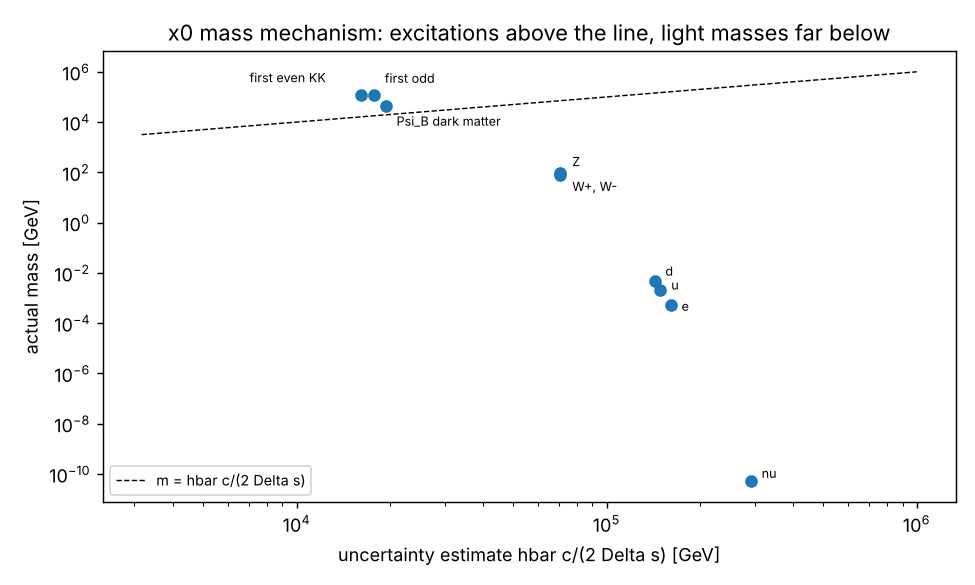
\includegraphics{figures/fig_analysis_heisenberg.png}
\caption{The \(x_0\) mass mechanism: the actual masses against the
uncertainty estimate \(m_{\mathrm{Heis}} = \hbar/(2\Delta(fy))\)
(circles: bosons and dirac16complex; squares: the twelve fermions, with
the \(m_{\mathrm{Heis}}\) of their broader zero mode); the excitations
and the dark matter lie above the line \(m = m_{\mathrm{Heis}}\), the
light particles far below. The axis labels are in the plain-text
notation of the plotting script: ``hbar c/(2 Delta s)'' is
\(m_{\mathrm{Heis}}\) and ``m\_H'' is \(m_{\mathrm{Heis}}\).}
\end{figure}

\hypertarget{why-the-light-fermions-must-be-zero-modes-whose-masses-come-from-the-tip-derived}{%
\subsubsection*{Why the light fermions must be zero modes whose masses
come from the tip
(DERIVED)}\label{why-the-light-fermions-must-be-zero-modes-whose-masses-come-from-the-tip-derived}}
\addcontentsline{toc}{subsubsection}{Why the light fermions must be zero
modes whose masses come from the tip (DERIVED)}

The lower bound of section A.4 makes the argument quantitative. The
hidden kinetic energy of any profile on the cell that is negligible at
the tip is at least that of a mass
\(m_{\mathrm{Heis}} \ge 1/(2fL) = 11.05\) TeV; for the actual zero modes
it is that of \(54\) to \(548\) TeV. Every observed fermion mass is at
least 64 times smaller than \(11.05\) TeV (the top quark) and up to
\(10^{16}\) times smaller (the lightest neutrino). A light fermion is
therefore possible only if the other terms of its \(x_0\) operator
cancel its hidden kinetic energy, and the cancellation must be exact up
to the tiny remainder: the profile must be an exact zero mode of the
\(x_0\) operator. The chiral zero modes of (FE-57) are exactly such
profiles: \(h\chi = 0\) at \(k = 0\), so the kinetic term \(c^2\) and
the bulk term \(c^2\) are cancelled by the boundary term \(-2c^2\), for
every localisation. They are ``flat relative to the geometry'' in the
same sense as the flat profile of the photon: in
\(\chi = \mathrm{e}^{c\xi}(1, 0)^T\) the whole \(x_0\) dependence is the
exponential that the bulk mass itself generates, and it costs no
four-dimensional energy. A zero mode is massless and chiral; a mass
requires a term that couples the doublet zero mode to a singlet zero
mode of the opposite chirality, and in UM-2 the only such term is the
tip Yukawa coupling of the sigma field (the tip conditions (FE-30)). The
mass it produces is proportional to the product of the amplitudes of the
two zero modes at the tip: this is the first-order root of the exact
mass condition, written out again:

\[
\begin{aligned}
&\mathcal{D}(\tilde\varepsilon) =
 \tilde\varepsilon^2\,\frac{\sinh\upsilon_L}{\upsilon_L}\frac{\sinh\upsilon_R}{\upsilon_R}
 - \mathcal{K}^2\Big(\cosh\upsilon_L - c_L\frac{\sinh\upsilon_L}{\upsilon_L}\Big)
 \Big(\cosh\upsilon_R + c_R\frac{\sinh\upsilon_R}{\upsilon_R}\Big) = 0,\\
&\tilde\varepsilon \simeq \mathcal{K}\,\mathcal{Z}(c_L)\,\mathcal{Z}(-c_R),\qquad \mathcal{Z}(c)^2 =
 \frac{c\,\mathrm{e}^{-c}}{\sinh c}
\end{aligned} \tag{FE-59}
\] \textbf{Symbols in (FE-59).}

\begin{itemize}
\tightlist
\item
  \(\mathcal{D}(\tilde\varepsilon)\): The mass function of one
  generation: its zeros are the dimensionless masses
  \(\tilde\varepsilon\). Unit: dimensionless. Status: DERIVED.
\item
  \(\tilde\varepsilon\): The dimensionless energy (mass) of a fermion
  mode, \(\tilde\varepsilon = \varepsilon fL\). Unit: dimensionless.
  Status: DERIVED.
\item
  \(\upsilon_L,\ \upsilon_R\): The auxiliary roots
  \(\upsilon = (c^2 - \tilde\varepsilon^2)^{1/2}\) of the doublet
  (\(\upsilon_L\)) and singlet (\(\upsilon_R\)) solutions at \(k = 0\).
  Unit: dimensionless. Status: DERIVED.
\item
  \(L\): The chirality label L: the left-handed (doublet) zero mode, or
  the left-handed projection \(P_L = (1 + \Gamma_4)/2\). Status:
  STANDARD.
\item
  \(R\): The chirality label R: the right-handed (singlet) zero mode or
  field, or the projection \(P_R = (1 - \Gamma_4)/2\). Status: STANDARD.
\item
  \(\mathcal{K}\): The tip mixing matrix of a sector in the boundary
  conditions of the fermion zero modes (a number \(\mathcal{K}\) for one
  generation, a \(3 \times 3\) matrix for three): \(\mathcal{K}_\nu\),
  \(\mathcal{K}_e\), \(\mathcal{K}_u\), \(\mathcal{K}_d\) of the
  neutrino, charged-lepton, up-quark and down-quark sectors; UM-2 takes
  \(\mathcal{K}_e = \mathcal{K}_u = \mathbf{1}\),
  \(\mathcal{K}_\nu = U\), \(\mathcal{K}_d = V_{\mathrm{CKM}}\). Unit:
  dimensionless. Status: ASSUMED.
\item
  \(c,\ c_L,\ c_R\): The localisation of a zero mode, \(c = f\mu L\)
  (bulk mass times the proper depth); \(c_L\) of a doublet (localised at
  the fold for \(c_L > 0\)), \(c_R\) of a singlet (localised at the fold
  for \(c_R < 0\)). Unit: dimensionless. Value: doublets
  \(c_L = 3.38230\) (quarks) and 5.95288 (leptons); singlets \(c_R\): up
  \(-15.4300\), down \(-14.6258\), strange \(-11.5158\), charm
  \(-8.7683\), bottom \(-7.5005\), top \(-3.3823\), electron
  \(-14.5539\), muon \(-8.9809\), tau \(-5.9529\), neutrinos
  \(-35.0452\), \(-32.8481\), \(-31.0702\) (fixed by the measured
  masses). Status: DERIVED.
\item
  \(\mathcal{Z}(c)\): The tip amplitude of a normalised zero mode with
  the localisation \(c\),
  \(\mathcal{Z}(c)^2 = c\,\mathrm{e}^{-c}/\sinh c\). Unit:
  dimensionless. Status: DERIVED.
\item
  \(\mathrm{e}\): Euler's number, the base of the natural logarithm;
  \(\mathrm{e}^{X}\) is the exponential of \(X\). Unit: dimensionless.
  Value: 2.718281828. Status: STANDARD.
\end{itemize}

For \(c \gg 1\) the tip density of a zero mode is exponentially small,
and so are the masses and their sensitivities to the localisation:

\[ \mathcal{Z}(c)^2 = \frac{c\,\mathrm{e}^{-c}}{\sinh c} \simeq 2c\,\mathrm{e}^{-2c},\qquad m = \frac{\tilde\varepsilon}{fL},\qquad \frac{\mathrm{d}\ln m}{\mathrm{d}\ln c} = \frac12\,\frac{\mathrm{d}\ln\mathcal{Z}(c)^2}{\mathrm{d}\ln c} \simeq \frac12 - c\qquad (c \gg 1) \]
\textbf{Symbols in this equation.}

\begin{itemize}
\tightlist
\item
  \(\mathcal{Z}(c)\): The tip amplitude of a normalised zero mode with
  the localisation \(c\),
  \(\mathcal{Z}(c)^2 = c\,\mathrm{e}^{-c}/\sinh c\). Unit:
  dimensionless. Status: DERIVED.
\item
  \(c,\ c_L,\ c_R\): The localisation of a zero mode, \(c = f\mu L\)
  (bulk mass times the proper depth); \(c_L\) of a doublet (localised at
  the fold for \(c_L > 0\)), \(c_R\) of a singlet (localised at the fold
  for \(c_R < 0\)). Unit: dimensionless. Value: doublets
  \(c_L = 3.38230\) (quarks) and 5.95288 (leptons); singlets \(c_R\): up
  \(-15.4300\), down \(-14.6258\), strange \(-11.5158\), charm
  \(-8.7683\), bottom \(-7.5005\), top \(-3.3823\), electron
  \(-14.5539\), muon \(-8.9809\), tau \(-5.9529\), neutrinos
  \(-35.0452\), \(-32.8481\), \(-31.0702\) (fixed by the measured
  masses). Status: DERIVED.
\item
  \(\mathrm{e}\): Euler's number, the base of the natural logarithm;
  \(\mathrm{e}^{X}\) is the exponential of \(X\). Unit: dimensionless.
  Value: 2.718281828. Status: STANDARD.
\item
  \(m,\ m_s,\ m_i\): A four-dimensional mass: \(m\) the mass of a mode
  (the eigenvalue of an \(x_0\) problem) or of a fermion; \(m_s\) the
  mass of the species \(s\); \(m_i\) the mass of the neutrino mass state
  \(i\). Unit: GeV. Status: DERIVED.
\item
  \(\tilde\varepsilon\): The dimensionless energy (mass) of a fermion
  mode, \(\tilde\varepsilon = \varepsilon fL\). Unit: dimensionless.
  Status: DERIVED.
\item
  \(f\): The block scale: the common scale factor of the hidden
  direction and the extra times, \(f = \mathrm{e}^{-a_4}b_4^{1/2}\) (the
  block is \(f^2\) times a four-dimensional space of constant curvature
  \(-H^2\)). Unit: dimensionless. Status: DERIVED.
\item
  \(L\): The depth of the regular tip: each half of a period of \(x_0\)
  ends at \(y = -L\); \(HL = 3\). Unit: length. Value: \(L = 3/H\)
  (\(fL = 8.926\times10^{-21}\) m at the stabilised block). Status:
  ASSUMED.
\item
  \(\mathrm{d}\): The differential: \(\mathrm{d}X\) is an infinitesimal
  change of \(X\), \(\mathrm{d}X/\mathrm{d}Y\) the derivative of \(X\)
  with respect to \(Y\), \(\mathrm{d}^nX\) the volume element of \(n\)
  variables. Status: STANDARD.
\end{itemize}

(\(c = -c_R\) for a singlet with the doublet fixed; \(-34.55\) for the
\(\nu_1\) singlet, \(-2.89\) for the top singlet). The masses of the
light fermions are thus tip effects of zero modes, not localisation
energies: the uncertainty relation does not produce them, and a sharper
localisation lowers them. The same holds for \(W^\pm\) and \(Z\), whose
profiles are the photon's flat zero mode bent by the tip parameter
\(\beta\): their masses are the small tip-induced bending
(\(m/m_{\mathrm{Heis}} \approx 10^{-3}\)).

\hypertarget{the-hierarchy-of-the-masses-derived}{%
\subsubsection*{The hierarchy of the masses
(DERIVED)}\label{the-hierarchy-of-the-masses-derived}}
\addcontentsline{toc}{subsubsection}{The hierarchy of the masses
(DERIVED)}

Because the tip densities depend exponentially on the localisations,
bulk masses of order one produce the whole hierarchy: the twelve fermion
masses span fourteen orders of magnitude, from \(\nu_1\) to the top
quark, with bulk masses between \(5.2H\) (the quark doublets,
\(\mu_Q = 5.2304\,H\)) and \(54.2H\) in magnitude (the \(\nu_1\)
singlet), and within a sector the lighter fermion has the sharper
singlet localisation. The doublet bulk masses are
\(\mu_\ell = 9.2055\,H\) and \(\mu_Q = 5.2304\,H\). The first-order root
of (FE-59) agrees with the exact roots to \(1.1\times10^{-3}\) for the
top quark and to better than \(3\times10^{-4}\) for every other fermion.
The hierarchy is the exponential response of the tip densities to
order-one bulk masses; it is not explained further by the mechanism (the
bulk masses are fitted).

\hypertarget{the-mixing-matrices-derived-assumed-inputs}{%
\subsubsection*{The mixing matrices (DERIVED, ASSUMED
inputs)}\label{the-mixing-matrices-derived-assumed-inputs}}
\addcontentsline{toc}{subsubsection}{The mixing matrices (DERIVED,
ASSUMED inputs)}

With the doublet shared by the three generations of a sector, the
charged current between the mass states \(\nu_j\) and the charged
leptons of the generation \(i\) carries
\(\sum_\alpha(\mathcal{K}_\nu)^*_{\alpha j}(\mathcal{K}_e)_{\alpha i}\),
and the mixing matrices are the tip matrices (from (FE-60)):

\[ U = \mathcal{K}_e^\dagger\mathcal{K}_\nu = \mathcal{K}_\nu,\qquad V_{\mathrm{CKM}} = \mathcal{K}_u^\dagger\mathcal{K}_d = \mathcal{K}_d\qquad (\mathcal{K}_e = \mathcal{K}_u = \mathbf{1}) \]
\textbf{Symbols in this equation.}

\begin{itemize}
\tightlist
\item
  \(U\): The PMNS matrix, the unitary \(3 \times 3\) mixing matrix of
  the leptons, \(\nu_\alpha = \sum_iU_{\alpha i}\nu_i\) (rows
  \(\alpha = e, \mu, \tau\), columns the mass states \(i\)); in UM-2
  \(U = \mathcal{K}_e^\dagger\mathcal{K}_\nu\). Unit: dimensionless.
  Value: \(\sin^2\theta_{12} = 0.308\), \(\sin^2\theta_{13} = 0.02215\),
  \(\sin^2\theta_{23} = 0.470\), \(\delta_{\mathrm{CP}} = 212^\circ\)
  (NuFIT 6.0). Status: STANDARD.
\item
  \(\mathcal{K}\): The tip mixing matrix of a sector in the boundary
  conditions of the fermion zero modes (a number \(\mathcal{K}\) for one
  generation, a \(3 \times 3\) matrix for three): \(\mathcal{K}_\nu\),
  \(\mathcal{K}_e\), \(\mathcal{K}_u\), \(\mathcal{K}_d\) of the
  neutrino, charged-lepton, up-quark and down-quark sectors; UM-2 takes
  \(\mathcal{K}_e = \mathcal{K}_u = \mathbf{1}\),
  \(\mathcal{K}_\nu = U\), \(\mathcal{K}_d = V_{\mathrm{CKM}}\). Unit:
  dimensionless. Status: ASSUMED.
\item
  \({}^\dagger\): Hermitian conjugation: the complex conjugate of the
  transpose of a matrix or spinor (for field operators the adjoint
  operator). Status: STANDARD.
\item
  \(V_{\mathrm{CKM}}\): The CKM matrix, the unitary \(3 \times 3\)
  mixing matrix of the quarks (the same parametrisation as \(U\)); in
  UM-2 \(V_{\mathrm{CKM}} = \mathcal{K}_u^\dagger\mathcal{K}_d\). Unit:
  dimensionless. Value: \(s_{12} = 0.22501\), \(s_{13} = 0.003732\),
  \(s_{23} = 0.04183\), \(\delta = 1.147\) (PDG). Status: STANDARD.
\item
  \(\mathbf{1}\): The identity matrix (of the size fixed by the context:
  16 x 16 on spinors, 3 x 3 on the generations or flavours, 2 x 2 for
  the sigma field). Unit: dimensionless. Status: STANDARD.
\end{itemize}

in the standard parametrisation (STANDARD; the same form for
\(V_{\mathrm{CKM}}\))

\[
\begin{aligned}
U = \begin{pmatrix} c_{12}c_{13} & s_{12}c_{13} & s_{13}\mathrm{e}^{-\mathrm{i}\delta_{\mathrm{CP}}}\\
 -s_{12}c_{23} - c_{12}s_{23}s_{13}\mathrm{e}^{\mathrm{i}\delta_{\mathrm{CP}}} &
 c_{12}c_{23} - s_{12}s_{23}s_{13}\mathrm{e}^{\mathrm{i}\delta_{\mathrm{CP}}} & s_{23}c_{13}\\
 s_{12}s_{23} - c_{12}c_{23}s_{13}\mathrm{e}^{\mathrm{i}\delta_{\mathrm{CP}}} &
 -c_{12}s_{23} - s_{12}c_{23}s_{13}\mathrm{e}^{\mathrm{i}\delta_{\mathrm{CP}}} &
 c_{23}c_{13}\end{pmatrix},\qquad
J_{\mathrm{CP}} = c_{12}s_{12}c_{23}s_{23}c_{13}^2s_{13}\sin\delta_{\mathrm{CP}}
\end{aligned} \tag{FE-61}
\] \textbf{Symbols in (FE-61).}

\begin{itemize}
\tightlist
\item
  \(U\): The PMNS matrix, the unitary \(3 \times 3\) mixing matrix of
  the leptons, \(\nu_\alpha = \sum_iU_{\alpha i}\nu_i\) (rows
  \(\alpha = e, \mu, \tau\), columns the mass states \(i\)); in UM-2
  \(U = \mathcal{K}_e^\dagger\mathcal{K}_\nu\). Unit: dimensionless.
  Value: \(\sin^2\theta_{12} = 0.308\), \(\sin^2\theta_{13} = 0.02215\),
  \(\sin^2\theta_{23} = 0.470\), \(\delta_{\mathrm{CP}} = 212^\circ\)
  (NuFIT 6.0). Status: STANDARD.
\item
  \(c_{12},\ c_{13},\ c_{23}\): The cosines of the mixing angles,
  \(c_{ij} = \cos\theta_{ij}\). Unit: dimensionless. Status: STANDARD.
\item
  \(s_{12},\ s_{13},\ s_{23}\): The sines of the mixing angles,
  \(s_{ij} = \sin\theta_{ij}\). Unit: dimensionless. Status: STANDARD.
\item
  \(\mathrm{e}\): Euler's number, the base of the natural logarithm;
  \(\mathrm{e}^{X}\) is the exponential of \(X\). Unit: dimensionless.
  Value: 2.718281828. Status: STANDARD.
\item
  \(\mathrm{i}\): The imaginary unit, \(\mathrm{i}^2 = -1\). Unit:
  dimensionless. Status: STANDARD.
\item
  \(\delta_{\mathrm{CP}}\): The CP-violating phase of a mixing matrix.
  Unit: dimensionless. Value: \(212^\circ\) (PMNS), 1.147 rad (CKM).
  Status: STANDARD.
\item
  \(J_{\mathrm{CP}}\): The Jarlskog invariant of a mixing matrix (the
  measure of CP violation). Unit: dimensionless. Value: \(-0.01777\)
  (PMNS), \(3.117\times10^{-5}\) (CKM). Status: STANDARD.
\end{itemize}

with \(\sin^2\theta_{12} = 0.308\), \(\sin^2\theta_{23} = 0.470\),
\(\sin^2\theta_{13} = 0.02215\), \(\delta_{\mathrm{CP}} = 212^\circ\)
for the PMNS matrix (NuFIT 6.0, normal ordering;
\(J_{\mathrm{CP}} = -0.01777\)) and \(s_{12} = 0.22501\),
\(s_{13} = 0.003732\), \(s_{23} = 0.04183\),
\(\delta_{\mathrm{CP}} = 1.147\) for the CKM matrix (PDG global fit;
\(J_{\mathrm{CP}} = 3.117\times10^{-5}\)), both unitary to
\(1.1\times10^{-16}\):

\[ \lvert U\rvert = \begin{pmatrix} 0.8226 & 0.5488 & 0.1488\\ 0.3351 & 0.6543 & 0.6779\\ 0.4594 & 0.5203 & 0.7199\end{pmatrix},\qquad \lvert V_{\mathrm{CKM}}\rvert = \begin{pmatrix} 0.97435 & 0.22501 & 0.00373\\ 0.22488 & 0.97349 & 0.04183\\ 0.00858 & 0.04111 & 0.99912\end{pmatrix} \]
\textbf{Symbols in this equation.}

\begin{itemize}
\tightlist
\item
  \(U\): The PMNS matrix, the unitary \(3 \times 3\) mixing matrix of
  the leptons, \(\nu_\alpha = \sum_iU_{\alpha i}\nu_i\) (rows
  \(\alpha = e, \mu, \tau\), columns the mass states \(i\)); in UM-2
  \(U = \mathcal{K}_e^\dagger\mathcal{K}_\nu\). Unit: dimensionless.
  Value: \(\sin^2\theta_{12} = 0.308\), \(\sin^2\theta_{13} = 0.02215\),
  \(\sin^2\theta_{23} = 0.470\), \(\delta_{\mathrm{CP}} = 212^\circ\)
  (NuFIT 6.0). Status: STANDARD.
\item
  \(V_{\mathrm{CKM}}\): The CKM matrix, the unitary \(3 \times 3\)
  mixing matrix of the quarks (the same parametrisation as \(U\)); in
  UM-2 \(V_{\mathrm{CKM}} = \mathcal{K}_u^\dagger\mathcal{K}_d\). Unit:
  dimensionless. Value: \(s_{12} = 0.22501\), \(s_{13} = 0.003732\),
  \(s_{23} = 0.04183\), \(\delta = 1.147\) (PDG). Status: STANDARD.
\end{itemize}

The angles and phases are inputs of UM-2, not predictions: the mechanism
explains the masses through the localisations, but not the mixing, which
is the choice of the tip matrices (OPEN: their origin). The right-handed
rotations are trivial, and because the doublets of a sector share one
bulk mass the first even Kaluza-Klein gauge mode couples to every
left-handed lepton with the same relative strength \(0.14434\) and to
every left-handed quark with \(-0.30066\), so there are no
flavour-changing neutral currents at tree level (the largest
off-diagonal coupling in the mass basis is \(10^{-17}\), round-off;
different doublet bulk masses would create off-diagonal couplings up to
\(0.033\)) (DERIVED).

\hypertarget{the-massless-zero-modes-derived}{%
\subsubsection*{The massless zero modes
(DERIVED)}\label{the-massless-zero-modes-derived}}
\addcontentsline{toc}{subsubsection}{The massless zero modes (DERIVED)}

The exactly massless states of UM-2 are the zero modes of \(x_0\)
operators that no term of the action lifts: the photon and the gluons
(flat profiles with \(\beta = 0\), protected by the unbroken gauge
invariance; the tip terms give mass to \(W^\pm\) and \(Z\) only), the
graviton (flat profile, protected by four-dimensional general
covariance), and the fold bands of both halves of dirac16complex (chiral
zero modes; no tip operator acts on them, the scalar density of a chiral
zero mode vanishes, and I13 acts only on the lower component; part B).
These are exactly the exceptions named by the author: the graviton, the
photon and the quanta of dirac16complex, more precisely its massless
fold bands, while its odd quanta are massive (the dark matter).

\hypertarget{a.6-proper-versus-coordinate-localisation-derived}{%
\subsection*{A.6 Proper versus coordinate localisation
(DERIVED)}\label{a.6-proper-versus-coordinate-localisation-derived}}
\addcontentsline{toc}{subsection}{A.6 Proper versus coordinate
localisation (DERIVED)}

The proper element of the hidden direction is

\[ f\,\mathrm{d}y = f\cot z\,\mathrm{d}x_0 \] \textbf{Symbols in this
equation.}

\begin{itemize}
\tightlist
\item
  \(f\): The block scale: the common scale factor of the hidden
  direction and the extra times, \(f = \mathrm{e}^{-a_4}b_4^{1/2}\) (the
  block is \(f^2\) times a four-dimensional space of constant curvature
  \(-H^2\)). Unit: dimensionless. Status: DERIVED.
\item
  \(\mathrm{d}\): The differential: \(\mathrm{d}X\) is an infinitesimal
  change of \(X\), \(\mathrm{d}X/\mathrm{d}Y\) the derivative of \(X\)
  with respect to \(Y\), \(\mathrm{d}^nX\) the volume element of \(n\)
  variables. Status: STANDARD.
\item
  \(y\): The hidden coordinate of the \(y\) chart,
  \(y = \ln\lvert\sin z\rvert/(6H)\), with \(y = 0\) at the fold
  (\(z = \pi/2\)) and \(y = -L\) at the regular tip; each half of a
  period of \(x_0\) is the interval \(-L \le y \le 0\). Unit: length.
  Status: DERIVED.
\item
  \(z\): The angle variable of the hidden direction, \(z = 6Hx_0\); one
  period of \(x_0\) is \(0 < z < \pi\). Unit: dimensionless. Status:
  AUTHOR.
\item
  \(x_0\): The hidden space-like coordinate (listed first); the metric
  depends on it through \(z = 6Hx_0\), periodically with the period
  \(\pi/(6H)\). Unit: length. Status: AUTHOR.
\end{itemize}

which vanishes at the fold and diverges at the tips. The photon zero
mode, localised at the fold in proper length, has 61.9 \% of its
probability within \(\pi/8\) of the tips in the coordinate
\(z = 6Hx_0\): localisation in the coordinate \(x_0\) is chart
dependent. A profile confined to a small proper distance from the fold
(\(\Delta\xi = 0.157\), i.e.~\(\lvert y\rvert \lesssim 0.47/H\),
\(\sin z \gtrsim \mathrm{e}^{-2.8}\)) extends over almost the whole
coordinate range of \(z\), and its probability per unit \(z\) is largest
near the tips. Only the proper hidden length enters the masses; the
author's ``\(\Delta x_0\) small'' must be read as ``\(\Delta(fy)\)
small''.

\hypertarget{a.7-the-neutrinos-masses-mixing-and-flavour-conversion-as-x_0-effects}{%
\subsection*{\texorpdfstring{A.7 The neutrinos: masses, mixing and
flavour conversion as \(x_0\)
effects}{A.7 The neutrinos: masses, mixing and flavour conversion as x\_0 effects}}\label{a.7-the-neutrinos-masses-mixing-and-flavour-conversion-as-x_0-effects}}
\addcontentsline{toc}{subsection}{A.7 The neutrinos: masses, mixing and
flavour conversion as \(x_0\) effects}

The three neutrino masses are \(x_0\) eigenvalues of the same kind as
the charged-fermion masses: Dirac masses produced at the tip by the
overlap of the lepton-doublet zero mode (\(c_\ell = 5.9529\)) with three
right-handed singlet zero modes localised very sharply at the fold
(\(c_R = -35.05\), \(-32.85\), \(-31.07\)). With the lightest mass
ASSUMED and the measured splittings (STANDARD, NuFIT 6.0, normal
ordering):

\[
m_1 = 1.000\ \text{meV},\qquad m_2 = \sqrt{m_1^2 + \Delta m_{21}^2} = 8.712\ \text{meV},\qquad
m_3 = \sqrt{m_1^2 + \Delta m_{31}^2} = 50.140\ \text{meV} \tag{FE-100}
\] \textbf{Symbols in (FE-100).}

\begin{itemize}
\tightlist
\item
  \(m_1,\ m_2,\ m_3\): The masses of the neutrino mass states \(\nu_1\),
  \(\nu_2\), \(\nu_3\) (normal ordering). Unit: GeV (quoted in meV).
  Value: 1.000, 8.712, 50.140 meV (\(m_1\) ASSUMED). Status: DERIVED.
\item
  \(\Delta\): The change (difference or small perturbation) of the
  quantity that follows: \(\Delta K\), \(\Delta\rho\), \(\Delta p_3\)
  are first-order changes about the static block,
  \(\Delta\varepsilon_o\) a level shift,
  \(\Delta m^2_{21} = m_2^2 - m_1^2\) a difference of squared masses,
  \(\Delta N_{\mathrm{eff}}\) an addition to \(N_{\mathrm{eff}}\),
  \(\Delta S_{\mathrm{m}}\) the change of an action under a change
  \(\Delta g^{MN}\) of the metric. Status: STANDARD.
\item
  \(\Delta m_{21}^2,\ \Delta m_{31}^2,\ \Delta m_{32}^2\): The
  differences of the squared neutrino masses,
  \(\Delta m_{ij}^2 = m_i^2 - m_j^2\). Unit: \(\mathrm{GeV}^{2}\)
  (quoted in \(\mathrm{eV}^{2}\)). Value:
  \(\Delta m_{21}^2 = 7.49\times10^{-5}\) eV\(^2\),
  \(\Delta m_{31}^2 = 2.513\times10^{-3}\) eV\(^2\) (NuFIT 6.0). Status:
  STANDARD.
\end{itemize}

The right-handed neutrinos are gauge singlets and are never in thermal
equilibrium (their interactions are the tip mixing, whose rate is
suppressed by \((m_i/T)^2\), STANDARD, and the portal I11 with the
\(B - L\) charge \(-1\), through which the dark matter annihilates into
right-handed neutrino pairs at only \(2.0\times10^{-17}\) of its I13
rate into quarks, DERIVED; part B), so they add no radiation. The PMNS
matrix is the tip matrix \(\mathcal{K}_\nu\) (section A.5); its angles
and phase are inputs. Given the masses and \(U\), the flavour conversion
follows from the four-dimensional effective theory (STANDARD):

\[
\mathrm{i}\,\frac{\mathrm{d}\boldsymbol{\psi}}{\mathrm{d}x_4} = H_{\mathrm{fl}}\,\boldsymbol{\psi},\qquad
H_{\mathrm{fl}} = \frac{1}{2E}\,U\,\mathrm{diag}\big(m_1^2,\ m_2^2,\ m_3^2\big)\,U^\dagger + V,\qquad
\mathcal{U}(L_{\mathrm{b}}) = \mathrm{e}^{-\mathrm{i}H_{\mathrm{fl}}L_{\mathrm{b}}},\qquad
\mathcal{P}(\nu_\alpha\to\nu_\beta) = \lvert\mathcal{U}_{\beta\alpha}\rvert^2 \tag{FE-104}
\] \textbf{Symbols in (FE-104).}

\begin{itemize}
\tightlist
\item
  \(\mathrm{i}\): The imaginary unit, \(\mathrm{i}^2 = -1\). Unit:
  dimensionless. Status: STANDARD.
\item
  \(\mathrm{d}\): The differential: \(\mathrm{d}X\) is an infinitesimal
  change of \(X\), \(\mathrm{d}X/\mathrm{d}Y\) the derivative of \(X\)
  with respect to \(Y\), \(\mathrm{d}^nX\) the volume element of \(n\)
  variables. Status: STANDARD.
\item
  \(\boldsymbol{\psi}\): The vector of the three flavour amplitudes of a
  neutrino. Unit: dimensionless. Status: STANDARD.
\item
  \(x_4\): The time; dots denote \(\mathrm{d}/\mathrm{d}x_4\). Unit:
  length (= time, c = 1). Status: AUTHOR.
\item
  \(H_{\mathrm{fl}}\): The flavour Hamiltonian of a neutrino of energy
  \(E\) (vacuum mass term plus matter potential). Unit: GeV. Status:
  STANDARD.
\item
  \(E\): The energy of a particle: of the neutrino in the flavour
  equations, \(E = (k^2 + m^2)^{1/2}\) of a particle of momentum \(k\)
  in the thermal integrals. Unit: GeV. Status: STANDARD.
\item
  \(U\): The PMNS matrix, the unitary \(3 \times 3\) mixing matrix of
  the leptons, \(\nu_\alpha = \sum_iU_{\alpha i}\nu_i\) (rows
  \(\alpha = e, \mu, \tau\), columns the mass states \(i\)); in UM-2
  \(U = \mathcal{K}_e^\dagger\mathcal{K}_\nu\). Unit: dimensionless.
  Value: \(\sin^2\theta_{12} = 0.308\), \(\sin^2\theta_{13} = 0.02215\),
  \(\sin^2\theta_{23} = 0.470\), \(\delta_{\mathrm{CP}} = 212^\circ\)
  (NuFIT 6.0). Status: STANDARD.
\item
  \(\mathrm{diag}\): A diagonal matrix with the listed entries on its
  diagonal (in the order of the coordinates \(x_0, x_1, \dots, x_7\)
  when it is a tensor in eight dimensions). Status: STANDARD.
\item
  \(m_1,\ m_2,\ m_3\): The masses of the neutrino mass states \(\nu_1\),
  \(\nu_2\), \(\nu_3\) (normal ordering). Unit: GeV (quoted in meV).
  Value: 1.000, 8.712, 50.140 meV (\(m_1\) ASSUMED). Status: DERIVED.
\item
  \({}^\dagger\): Hermitian conjugation: the complex conjugate of the
  transpose of a matrix or spinor (for field operators the adjoint
  operator). Status: STANDARD.
\item
  \(V_\alpha,\ V\): The matter potential of forward scattering:
  \(V_\alpha\) of the flavour \(\alpha\) (\(V_e\), \(V_\mu\)), \(V\) the
  \(3 \times 3\) matrix of the potentials in the flavour basis;
  antineutrinos have \(-V\). Unit: GeV. Status: STANDARD.
\item
  \(\mathcal{U}\): The flavour evolution operator over the baseline
  \(L_{\mathrm{b}}\); \(\mathcal{U}_{\beta\alpha}\) the amplitude of
  \(\nu_\alpha \to \nu_\beta\). Unit: dimensionless. Status: STANDARD.
\item
  \(L_{\mathrm{b}}\): The baseline: the distance travelled by the
  neutrino. Unit: length. Status: STANDARD.
\item
  \(\mathrm{e}\): Euler's number, the base of the natural logarithm;
  \(\mathrm{e}^{X}\) is the exponential of \(X\). Unit: dimensionless.
  Value: 2.718281828. Status: STANDARD.
\item
  \(\mathcal{P}\): The probability of a flavour transition,
  \(\mathcal{P}(\nu_\alpha \to \nu_\beta)\); \(\mathcal{P}_{ee}\) the
  survival probability of electron neutrinos. Unit: dimensionless.
  Status: STANDARD.
\item
  \(\nu_\alpha,\ \nu_i\): A left-handed neutrino: \(\nu_\alpha\) of the
  flavour \(\alpha = e, \mu, \tau\) (\(\nu_e\), \(\nu_\mu\),
  \(\nu_\tau\)), \(\nu_i\) of the mass state \(i\) (mass \(m_i\)). Unit:
  \(\mathrm{GeV}^{3/2}\). Status: STANDARD.
\item
  \(\alpha\): A flavour index running over \(e, \mu, \tau\) (the flavour
  states of the leptons and neutrinos). Status: STANDARD.
\item
  \(\beta\): A second flavour index running over \(e, \mu, \tau\).
  Status: STANDARD.
\end{itemize}

with the potentials of coherent forward scattering in matter

\[
\begin{aligned}
&V_\alpha = \sqrt2\,G_{\mathrm{F}}\Big[\delta_{\alpha e}\big(n_{e^-} - n_{e^+}\big) + \sum_f\tilde
 g^f_V\big(n_f - n_{\bar f}\big)\Big],\\
&V = \mathrm{diag}\big(V_{\mathrm{CC}},\ 0,\ 0\big) + V_{\mathrm{NC}}\,\mathbf{1},\qquad V_{\mathrm{CC}}
 = \sqrt2\,G_{\mathrm{F}}\,n_{\mathrm{e}},
 \qquad V_{\mathrm{NC}} = -\frac{G_{\mathrm{F}}\,n_{\mathrm{n}}}{\sqrt2}
\end{aligned} \tag{FE-103}
\] \textbf{Symbols in (FE-103).}

\begin{itemize}
\tightlist
\item
  \(V_\alpha,\ V\): The matter potential of forward scattering:
  \(V_\alpha\) of the flavour \(\alpha\) (\(V_e\), \(V_\mu\)), \(V\) the
  \(3 \times 3\) matrix of the potentials in the flavour basis;
  antineutrinos have \(-V\). Unit: GeV. Status: STANDARD.
\item
  \(\alpha\): A flavour index running over \(e, \mu, \tau\) (the flavour
  states of the leptons and neutrinos). Status: STANDARD.
\item
  \(G_{\mathrm{F}}\): The Fermi constant. Unit: \(\mathrm{GeV}^{-2}\).
  Value: \(1.1663788\times10^{-5}\) GeV\(^{-2}\) (measured). Status:
  STANDARD.
\item
  \(\delta\): The Kronecker delta: with two indices \(\delta^M_N = 1\)
  if \(M = N\) and 0 otherwise (likewise \(\delta_{\alpha e}\),
  \(\delta_{l0}\), \(\delta^{I3}\)); with upper and lower index strings
  the generalised Kronecker delta
  \(\delta^{M_1\cdots M_n}_{N_1\cdots N_n}\), the determinant of the
  \(n \times n\) matrix of Kronecker deltas \(\delta^{M_a}_{N_b}\) (+1
  or -1 if the upper indices are an even or odd permutation of the lower
  ones, 0 otherwise). Status: STANDARD.
\item
  \(e\): The electron flavour as a value of a flavour index
  (\(\delta_{\alpha e}\), \(U_{e2}\), \(V_e\), \(\mathcal{P}_{ee}\)).
  Status: STANDARD.
\item
  \(n_{e^-},\ n_{e^+}\): The number densities of electrons and of
  positrons. Unit: \(\mathrm{GeV}^{3}\). Status: STANDARD.
\item
  \(f\): The label of a fermion species: a Standard-Model multiplet of
  one generation (its \(N_{\mathrm{c}}\) Weyl components share one
  zero-mode profile; the zero mode of each chirality) or a fermion of a
  medium (electron, proton, neutron); a sum over \(f\) runs over these
  species. Status: STANDARD.
\item
  \(\tilde g^f_L,\ \tilde g^f_R,\ \tilde g^f_V\): The neutral-current
  couplings of the fermion \(f\) to the \(Z\) (left-handed, right-handed
  and vector),
  \(\tilde g^f_L = T_3^f - Q^f_{\mathrm{em}}\sin^2\theta_{\mathrm{W}}\).
  Unit: dimensionless. Status: STANDARD.
\item
  \(V\): The label V of the vector coupling of a fermion to the \(Z\),
  \(\tilde g^f_V = \tilde g^f_L + \tilde g^f_R\). Status: STANDARD.
\item
  \(n,\ n_o,\ n_{\psi i},\ n_f,\ n_i\): A number density: \(n(y)\) the
  particle density of dirac16complex in the Kohn-Sham equations and
  \(n_o\) the contribution of the orbital \(o\), \(n_{\psi i}(y)\) the
  density of the Standard-Model fermion \(\psi_i\) (per proper 7-volume
  of eight dimensions); \(n_f\) the density of the fermion component
  \(f\) and \(n_i\) that of the neutrino mass state \(i\) (per 3-volume
  of four dimensions). Unit: \(\mathrm{GeV}^{7}\) (eight dimensions),
  \(\mathrm{GeV}^{3}\) (four dimensions). Status: STANDARD.
\item
  \(n_{\bar f}\): The number density of the antiparticles of the fermion
  \(f\). Unit: \(\mathrm{GeV}^{3}\). Status: STANDARD.
\item
  \(\mathrm{diag}\): A diagonal matrix with the listed entries on its
  diagonal (in the order of the coordinates \(x_0, x_1, \dots, x_7\)
  when it is a tensor in eight dimensions). Status: STANDARD.
\item
  \(V_{\mathrm{CC}},\ V_{\mathrm{NC}}\): The charged-current potential
  of electron neutrinos and the neutral-current potential common to all
  flavours. Unit: GeV. Status: STANDARD.
\item
  \(\mathbf{1}\): The identity matrix (of the size fixed by the context:
  16 x 16 on spinors, 3 x 3 on the generations or flavours, 2 x 2 for
  the sigma field). Unit: dimensionless. Status: STANDARD.
\item
  \(n_{\mathrm{e}}\): The number density of electrons (net of
  positrons); in the Thomson terms of the photon and baryon equations
  only free (ionised) electrons count. Unit: \(\mathrm{GeV}^{3}\).
  Status: STANDARD.
\item
  \(n_{\mathrm{n}}\): The number density of neutrons (free and bound).
  Unit: \(\mathrm{GeV}^{3}\). Status: STANDARD.
\end{itemize}

(the neutral-current potential is common to the three flavours and drops
out of the conversion; for antineutrinos \(U \to U^*\) and
\(V \to -V\)). The oscillation phases \(\Delta_{21}\), \(\Delta_{31}\),
\(\Delta_{32}\) contain the differences of squared \(x_0\) eigenvalues,
so oscillation experiments measure the \(x_0\) spectrum directly. These
differences are the quantities of UM-2 most sensitive to the block scale
(DERIVED):

\[ \begin{aligned} &\frac{\mathrm{d}\ln\big(m_j^2 - m_i^2\big)}{\mathrm{d}\ln f} = \frac{2}{m_j^2 - m_i^2}\Big(m_j^2\,\frac{\mathrm{d}\ln m_j}{\mathrm{d}\ln f} - m_i^2\,\frac{\mathrm{d}\ln m_i}{\mathrm{d}\ln f}\Big):\\
&\frac{\mathrm{d}\ln\Delta m_{21}^2}{\mathrm{d}\ln f} = -77.5,\qquad \frac{\mathrm{d}\ln\Delta m_{31}^2}{\mathrm{d}\ln f} = -74.0,\qquad \frac{\mathrm{d}\ln\Delta m_{32}^2}{\mathrm{d}\ln f} = -73.9 \end{aligned} \]
\textbf{Symbols in this equation.}

\begin{itemize}
\tightlist
\item
  \(\mathrm{d}\): The differential: \(\mathrm{d}X\) is an infinitesimal
  change of \(X\), \(\mathrm{d}X/\mathrm{d}Y\) the derivative of \(X\)
  with respect to \(Y\), \(\mathrm{d}^nX\) the volume element of \(n\)
  variables. Status: STANDARD.
\item
  \(m,\ m_s,\ m_i\): A four-dimensional mass: \(m\) the mass of a mode
  (the eigenvalue of an \(x_0\) problem) or of a fermion; \(m_s\) the
  mass of the species \(s\); \(m_i\) the mass of the neutrino mass state
  \(i\). Unit: GeV. Status: DERIVED.
\item
  \(j\): A second generation index (\(j = 1, 2, 3\)). Status: STANDARD.
\item
  \(i\): The generation index (\(i = 1, 2, 3\)), which also labels the
  neutrino mass states \(\nu_1, \nu_2, \nu_3\); a repeated index is not
  summed unless a sum sign is written. Status: STANDARD.
\item
  \(f\): The block scale: the common scale factor of the hidden
  direction and the extra times, \(f = \mathrm{e}^{-a_4}b_4^{1/2}\) (the
  block is \(f^2\) times a four-dimensional space of constant curvature
  \(-H^2\)). Unit: dimensionless. Status: DERIVED.
\item
  \(\Delta\): The change (difference or small perturbation) of the
  quantity that follows: \(\Delta K\), \(\Delta\rho\), \(\Delta p_3\)
  are first-order changes about the static block,
  \(\Delta\varepsilon_o\) a level shift,
  \(\Delta m^2_{21} = m_2^2 - m_1^2\) a difference of squared masses,
  \(\Delta N_{\mathrm{eff}}\) an addition to \(N_{\mathrm{eff}}\),
  \(\Delta S_{\mathrm{m}}\) the change of an action under a change
  \(\Delta g^{MN}\) of the metric. Status: STANDARD.
\item
  \(\Delta m_{21}^2,\ \Delta m_{31}^2,\ \Delta m_{32}^2\): The
  differences of the squared neutrino masses,
  \(\Delta m_{ij}^2 = m_i^2 - m_j^2\). Unit: \(\mathrm{GeV}^{2}\)
  (quoted in \(\mathrm{eV}^{2}\)). Value:
  \(\Delta m_{21}^2 = 7.49\times10^{-5}\) eV\(^2\),
  \(\Delta m_{31}^2 = 2.513\times10^{-3}\) eV\(^2\) (NuFIT 6.0). Status:
  STANDARD.
\end{itemize}

The light neutrino states also mix with the Kaluza-Klein excitations of
the lepton fields, which makes the \(3\times3\) PMNS matrix non-unitary
at the relative order \((m_i/m_{\mathrm{KK}})^2 \le 1.7\times10^{-31}\)
(ESTIMATE; \(2.0\times10^{-6}\) for the top quark, the largest of all
fermions): unobservable. The flavour conversion of UM-2 is therefore
that of the three-flavour Standard Model with Dirac neutrinos, which
UM-2 computes for the vacuum, the Earth, the Sun, the early Universe and
supernovae.

\textbf{Dirac or Majorana (DERIVED).} The \(x_0\) mechanism explains the
small Dirac masses by the localisation of the right-handed singlets with
tip couplings of order one. Without right-handed neutrinos the masses
would be Majorana masses from the gauge-invariant tip operator (the tip
form of the Weinberg operator; not part of UM-2)

\[ S_{\mathrm{M}} = -\frac12\int_{y=-L}\mathrm{d}^7X_{\mathrm{tip}}\sqrt{\lvert g_{\mathrm{tip}}\rvert}\,\sum_{i,j=1}^{3}m^{\mathrm{M}}_{ij}\,\tilde\nu_i\tilde\nu_j + \text{h.c.},\qquad \tilde\nu_i = \big(\Sigma^\dagger\ell_i\big)_1 \]
\textbf{Symbols in this equation.}

\begin{itemize}
\tightlist
\item
  \(S_{\mathrm{M}}\): The action of the gauge-invariant Majorana mass
  operator on the tip, the alternative to the Dirac neutrinos of UM-2
  without right-handed neutrinos (not part of UM-2). Unit: dimensionless
  (an action, \(\hbar = 1\)). Status: INVENTED.
\item
  \(y\): The hidden coordinate of the \(y\) chart,
  \(y = \ln\lvert\sin z\rvert/(6H)\), with \(y = 0\) at the fold
  (\(z = \pi/2\)) and \(y = -L\) at the regular tip; each half of a
  period of \(x_0\) is the interval \(-L \le y \le 0\). Unit: length.
  Status: DERIVED.
\item
  \(L\): The depth of the regular tip: each half of a period of \(x_0\)
  ends at \(y = -L\); \(HL = 3\). Unit: length. Value: \(L = 3/H\)
  (\(fL = 8.926\times10^{-21}\) m at the stabilised block). Status:
  ASSUMED.
\item
  \(\mathrm{d}\): The differential: \(\mathrm{d}X\) is an infinitesimal
  change of \(X\), \(\mathrm{d}X/\mathrm{d}Y\) the derivative of \(X\)
  with respect to \(Y\), \(\mathrm{d}^nX\) the volume element of \(n\)
  variables. Status: STANDARD.
\item
  \(X_{\mathrm{tip}}\): The seven coordinates \(x_1, \dots, x_7\) of the
  tip \(y = -L\) of the hidden direction;
  \(\mathrm{d}^7X_{\mathrm{tip}}\) is their coordinate volume element.
  Unit: length (each coordinate). Status: DERIVED.
\item
  \(g_{\mathrm{tip}}\): The metric induced on the seven-dimensional tip
  \(y = -L\) (the metric \(g_{MN}\) restricted to the tip directions
  \(x_1, \dots, x_7\)); \(\lvert g_{\mathrm{tip}}\rvert\) is the
  absolute value of its determinant. Unit: dimensionless. Status:
  DERIVED.
\item
  \(i\): The generation index (\(i = 1, 2, 3\)), which also labels the
  neutrino mass states \(\nu_1, \nu_2, \nu_3\); a repeated index is not
  summed unless a sum sign is written. Status: STANDARD.
\item
  \(j\): A second generation index (\(j = 1, 2, 3\)). Status: STANDARD.
\item
  \(m^{\mathrm{M}}_{ij}\): The complex symmetric \(3\times3\) matrix of
  the Majorana tip masses of the alternative operator \(S_{\mathrm{M}}\)
  (generation indices \(i\), \(j\)). Unit: GeV. Status: INVENTED.
\item
  \(\tilde\nu_i\): The neutral upper component
  \((\Sigma^\dagger\ell_i)_1\) of the lepton doublet of generation \(i\)
  dressed with the tip sigma field: a left-handed field that is neutral
  under \(SU(2)_L\times U(1)_Y\); \(\tilde\nu_i\tilde\nu_j\) is the
  Lorentz-invariant (Majorana) product of two such fields. Unit:
  \(\mathrm{GeV}^{7/2}\) (an eight-dimensional spinor field at the tip).
  Status: INVENTED.
\item
  \(\Sigma\): The tip sigma field: a unitary \(2 \times 2\) matrix field
  on the tip (\(\Sigma^\dagger\Sigma = \mathbf{1}\)) that replaces the
  Higgs doublet; its three modes are the longitudinal \(W^+\), \(W^-\)
  and \(Z\), and \(\Sigma = \mathbf{1}\) is the unitary gauge. Unit:
  dimensionless. Status: INVENTED.
\item
  \({}^\dagger\): Hermitian conjugation: the complex conjugate of the
  transpose of a matrix or spinor (for field operators the adjoint
  operator). Status: STANDARD.
\item
  \(\ell_i,\ \bar\ell_i\): The lepton doublet of the generation \(i\)
  (left-handed neutrino and charged lepton) and its Dirac adjoint. Unit:
  \(\mathrm{GeV}^{7/2}\). Status: ASSUMED.
\end{itemize}

(the upper component of \(\Sigma^\dagger\ell_i\) is neutral, since
\(\Sigma \to U_L\Sigma U_Y^\dagger\) absorbs both the SU(2) and the
hypercharge transformations of \(\ell_i\)), which gives, to first order
in the tip value of the doublet zero mode,

\[ m_i = \mathcal{K}_{\mathrm{M}}^{(i)}\,\frac{\mathcal{Z}(c_L)^2}{fL},\qquad \mathcal{Z}(c_L)^2 = 8.04\times10^{-5},\qquad \frac{1}{fL} = 22.11\ \text{TeV}, \]
\textbf{Symbols in this equation.}

\begin{itemize}
\tightlist
\item
  \(m,\ m_s,\ m_i\): A four-dimensional mass: \(m\) the mass of a mode
  (the eigenvalue of an \(x_0\) problem) or of a fermion; \(m_s\) the
  mass of the species \(s\); \(m_i\) the mass of the neutrino mass state
  \(i\). Unit: GeV. Status: DERIVED.
\item
  \(i\): The generation index (\(i = 1, 2, 3\)), which also labels the
  neutrino mass states \(\nu_1, \nu_2, \nu_3\); a repeated index is not
  summed unless a sum sign is written. Status: STANDARD.
\item
  \(\mathcal{K}_{\mathrm{M}}^{(i)}\): The dimensionless Majorana tip
  coefficient that the alternative would need for the mass state \(i\)
  (written with the index \(i\) in brackets):
  \(m_i = \mathcal{K}_{\mathrm{M}}^{(i)}\,\mathcal{Z}(c_L)^2/(fL)\) to
  first order in the tip value of the doublet zero mode. Unit:
  dimensionless. Value: \(5.63\times10^{-13}\), \(4.90\times10^{-12}\),
  \(2.82\times10^{-11}\) for \(i = 1, 2, 3\). Status: DERIVED.
\item
  \(\mathcal{Z}(c)\): The tip amplitude of a normalised zero mode with
  the localisation \(c\),
  \(\mathcal{Z}(c)^2 = c\,\mathrm{e}^{-c}/\sinh c\). Unit:
  dimensionless. Status: DERIVED.
\item
  \(c,\ c_L,\ c_R\): The localisation of a zero mode, \(c = f\mu L\)
  (bulk mass times the proper depth); \(c_L\) of a doublet (localised at
  the fold for \(c_L > 0\)), \(c_R\) of a singlet (localised at the fold
  for \(c_R < 0\)). Unit: dimensionless. Value: doublets
  \(c_L = 3.38230\) (quarks) and 5.95288 (leptons); singlets \(c_R\): up
  \(-15.4300\), down \(-14.6258\), strange \(-11.5158\), charm
  \(-8.7683\), bottom \(-7.5005\), top \(-3.3823\), electron
  \(-14.5539\), muon \(-8.9809\), tau \(-5.9529\), neutrinos
  \(-35.0452\), \(-32.8481\), \(-31.0702\) (fixed by the measured
  masses). Status: DERIVED.
\item
  \(L\): The chirality label L: the left-handed (doublet) zero mode, or
  the left-handed projection \(P_L = (1 + \Gamma_4)/2\). Status:
  STANDARD.
\item
  \(f\): The block scale: the common scale factor of the hidden
  direction and the extra times, \(f = \mathrm{e}^{-a_4}b_4^{1/2}\) (the
  block is \(f^2\) times a four-dimensional space of constant curvature
  \(-H^2\)). Unit: dimensionless. Status: DERIVED.
\item
  \(L\): The depth of the regular tip: each half of a period of \(x_0\)
  ends at \(y = -L\); \(HL = 3\). Unit: length. Value: \(L = 3/H\)
  (\(fL = 8.926\times10^{-21}\) m at the stabilised block). Status:
  ASSUMED.
\end{itemize}

so the measured masses need
\(\mathcal{K}_{\mathrm{M}}^{(i)} = 5.6\times10^{-13}\),
\(4.9\times10^{-12}\), \(2.8\times10^{-11}\): a hierarchy of tip
couplings that the mechanism does not explain. The \(x_0\) mechanism
therefore favours Dirac neutrinos. The Majorana case would show up in
neutrinoless double-beta decay with

\[ m_{\beta\beta} = \Big\lvert\sum_{i=1}^{3}U_{ei}^2\,m_i\,\mathrm{e}^{\mathrm{i}\varphi^{\mathrm{M}}_i}\Big\rvert \]
\textbf{Symbols in this equation.}

\begin{itemize}
\tightlist
\item
  \(m_{\beta\beta}\): The effective Majorana mass of neutrinoless
  double-beta decay,
  \(\lvert\sum_iU_{ei}^2m_i\mathrm{e}^{\mathrm{i}\varphi^{\mathrm{M}}_i}\rvert\).
  Unit: eV. Value: \(0.84\) to \(4.41\) meV over all Majorana phases.
  Status: DERIVED.
\item
  \(i\): The generation index (\(i = 1, 2, 3\)), which also labels the
  neutrino mass states \(\nu_1, \nu_2, \nu_3\); a repeated index is not
  summed unless a sum sign is written. Status: STANDARD.
\item
  \(U\): The PMNS matrix, the unitary \(3 \times 3\) mixing matrix of
  the leptons, \(\nu_\alpha = \sum_iU_{\alpha i}\nu_i\) (rows
  \(\alpha = e, \mu, \tau\), columns the mass states \(i\)); in UM-2
  \(U = \mathcal{K}_e^\dagger\mathcal{K}_\nu\). Unit: dimensionless.
  Value: \(\sin^2\theta_{12} = 0.308\), \(\sin^2\theta_{13} = 0.02215\),
  \(\sin^2\theta_{23} = 0.470\), \(\delta_{\mathrm{CP}} = 212^\circ\)
  (NuFIT 6.0). Status: STANDARD.
\item
  \(e\): The electron flavour as a value of a flavour index
  (\(\delta_{\alpha e}\), \(U_{e2}\), \(V_e\), \(\mathcal{P}_{ee}\)).
  Status: STANDARD.
\item
  \(m,\ m_s,\ m_i\): A four-dimensional mass: \(m\) the mass of a mode
  (the eigenvalue of an \(x_0\) problem) or of a fermion; \(m_s\) the
  mass of the species \(s\); \(m_i\) the mass of the neutrino mass state
  \(i\). Unit: GeV. Status: DERIVED.
\item
  \(\mathrm{e}\): Euler's number, the base of the natural logarithm;
  \(\mathrm{e}^{X}\) is the exponential of \(X\). Unit: dimensionless.
  Value: 2.718281828. Status: STANDARD.
\item
  \(\mathrm{i}\): The imaginary unit, \(\mathrm{i}^2 = -1\). Unit:
  dimensionless. Status: STANDARD.
\item
  \(\varphi^{\mathrm{M}}_i\): The Majorana phase of the neutrino mass
  state \(i\) in the Majorana alternative (a free parameter; all values
  are scanned). Unit: dimensionless (radians). Status: ASSUMED.
\end{itemize}

between \(0.84\) and \(4.41\) meV over all Majorana phases
(\(\lvert U_{ei}\rvert^2m_i = 0.677\), \(2.624\), \(1.111\) meV), below
the reach of present experiments, and in a twice larger capture rate of
the non-relativistic cosmic neutrino background; the flavour conversion
is the same.

\hypertarget{a.8-the-mass-mechanism-the-block-and-the-deflating-extra-times}{%
\subsection*{A.8 The mass mechanism, the block and the deflating extra
times}\label{a.8-the-mass-mechanism-the-block-and-the-deflating-extra-times}}
\addcontentsline{toc}{subsection}{A.8 The mass mechanism, the block and
the deflating extra times}

Every mass and coupling depends on the block scale \(f\) (DERIVED). A
fermion mass \(m = \tilde\varepsilon/(fL)\), with the first-order root
of (FE-59) and localisations \(c = f\mu L\) proportional to \(f\), has
the block sensitivity

\[
\frac{\mathrm{d}\ln m}{\mathrm{d}\ln f} = -1 +
 \frac12\Big[\frac{\mathrm{d}\ln\mathcal{Z}(c_L)^2}{\mathrm{d}\ln c_L}
 + \frac{\mathrm{d}\ln\mathcal{Z}(-c_R)^2}{\mathrm{d}\ln(-c_R)}\Big] \tag{FE-85}
\] \textbf{Symbols in (FE-85).}

\begin{itemize}
\tightlist
\item
  \(\mathrm{d}\): The differential: \(\mathrm{d}X\) is an infinitesimal
  change of \(X\), \(\mathrm{d}X/\mathrm{d}Y\) the derivative of \(X\)
  with respect to \(Y\), \(\mathrm{d}^nX\) the volume element of \(n\)
  variables. Status: STANDARD.
\item
  \(m,\ m_s,\ m_i\): A four-dimensional mass: \(m\) the mass of a mode
  (the eigenvalue of an \(x_0\) problem) or of a fermion; \(m_s\) the
  mass of the species \(s\); \(m_i\) the mass of the neutrino mass state
  \(i\). Unit: GeV. Status: DERIVED.
\item
  \(f\): The block scale: the common scale factor of the hidden
  direction and the extra times, \(f = \mathrm{e}^{-a_4}b_4^{1/2}\) (the
  block is \(f^2\) times a four-dimensional space of constant curvature
  \(-H^2\)). Unit: dimensionless. Status: DERIVED.
\item
  \(\mathcal{Z}(c)\): The tip amplitude of a normalised zero mode with
  the localisation \(c\),
  \(\mathcal{Z}(c)^2 = c\,\mathrm{e}^{-c}/\sinh c\). Unit:
  dimensionless. Status: DERIVED.
\item
  \(c,\ c_L,\ c_R\): The localisation of a zero mode, \(c = f\mu L\)
  (bulk mass times the proper depth); \(c_L\) of a doublet (localised at
  the fold for \(c_L > 0\)), \(c_R\) of a singlet (localised at the fold
  for \(c_R < 0\)). Unit: dimensionless. Value: doublets
  \(c_L = 3.38230\) (quarks) and 5.95288 (leptons); singlets \(c_R\): up
  \(-15.4300\), down \(-14.6258\), strange \(-11.5158\), charm
  \(-8.7683\), bottom \(-7.5005\), top \(-3.3823\), electron
  \(-14.5539\), muon \(-8.9809\), tau \(-5.9529\), neutrinos
  \(-35.0452\), \(-32.8481\), \(-31.0702\) (fixed by the measured
  masses). Status: DERIVED.
\item
  \(L\): The chirality label L: the left-handed (doublet) zero mode, or
  the left-handed projection \(P_L = (1 + \Gamma_4)/2\). Status:
  STANDARD.
\item
  \(R\): The chirality label R: the right-handed (singlet) zero mode or
  field, or the projection \(P_R = (1 - \Gamma_4)/2\). Status: STANDARD.
\end{itemize}

the Kaluza-Klein masses \(m^{\mathrm{KK}}_n = \tilde m_n/(fL)\) scale as
\(f^{-1}\), and the four-dimensional couplings and Newton's constant
follow from the reduction on the block

\[
\begin{aligned}
&G^{(4)}_{\mu\nu} + \Lambda_4\,g^{(4)}_{\mu\nu} = 8\pi G_{\mathrm{N}}\,\mathcal{T}^{(4)}_{\mu\nu},\qquad
 8\pi G_{\mathrm{N}} = \frac{\kappa}{\mathcal{G}(K_*)\,V_\perp},\qquad V_\perp =
 \frac{2f^4v_{\mathrm{t}}\big(1 - \mathrm{e}^{-3HL}\big)}{3H},\\
&\mathcal{T}^{(4)}_{\mu\nu} =
 \int\mathrm{d}x_0\,\mathrm{d}x_5\,\mathrm{d}x_6\,\mathrm{d}x_7\,\sqrt{\lvert
 g_\perp\rvert}\;\mathcal{T}_{\mu\nu},
 \qquad g_3^2 = \frac{\hat g_3^2}{V_\perp},\qquad g_2^2 = \frac{\hat g_2^2}{V_\perp},\qquad g_1^2 =
 \frac{\hat g_1^2}{V_\perp}
\end{aligned} \tag{FE-49}
\] \textbf{Symbols in (FE-49).}

\begin{itemize}
\tightlist
\item
  \(G^{(4)}_{\mu\nu}\): The Einstein tensor of the four-dimensional
  metric, \(R^{(4)}_{\mu\nu} - \frac12 g^{(4)}_{\mu\nu}R^{(4)}\). Unit:
  1/\(\mathrm{length}^{2}\). Status: STANDARD.
\item
  \(\mu\): A four-dimensional coordinate index running over the
  observable coordinates \(x_1, x_2, x_3, x_4\) (signature \(+,+,+,-\));
  on the tip it runs over the tip directions; a repeated index is
  summed. Status: STANDARD.
\item
  \(\nu\): A four-dimensional coordinate index running over
  \(x_1, \dots, x_4\) (as \(\mu\)). Status: STANDARD.
\item
  \(\Lambda_4\): The four-dimensional cosmological constant of the
  effective theory on the block,
  \(\Lambda_4 = [6H^2K(1 - 2w_{(2)}K) + \Lambda + \kappa\rho_{\mathrm{stab}}]/\mathcal{G}(K)\);
  zero at the static point, the observed dark energy a tuned residual.
  Unit: \(\mathrm{GeV}^{2}\). Value: 0 at the static point; observed
  \(\Lambda_4/H^2 \sim 10^{-92}\). Status: DERIVED.
\item
  \(g^{(4)}_{\mu\nu}\): The four-dimensional metric of the observable
  coordinates \(x_1, \dots, x_4\) (the metric of the effective
  four-dimensional general relativity on the stabilised block). Unit:
  dimensionless. Status: DERIVED.
\item
  \(\pi\): The number pi, the ratio of the circumference of a circle to
  its diameter. Unit: dimensionless. Value: 3.141592654. Status:
  STANDARD.
\item
  \(G_{\mathrm{N}}\): Newton's constant of four-dimensional gravity,
  \(8\pi G_{\mathrm{N}} = \kappa/(\mathcal{G}(K_*)V_\perp)\). Unit:
  \(\mathrm{GeV}^{-2}\). Value: \(6.709\times10^{-39}\) GeV\(^{-2}\)
  (\(M_{\mathrm{Pl}} = G_{\mathrm{N}}^{-1/2} = 1.22091\times10^{19}\)
  GeV). Status: STANDARD.
\item
  \(\mathcal{T}^{(4)}_{\mu\nu}\): The four-dimensional energy-momentum
  tensor: \(\mathcal{T}_{\mu\nu}\) integrated over the block (both
  halves of a period of \(x_0\) and the extra times). Unit:
  \(\mathrm{GeV}^{4}\). Status: DERIVED.
\item
  \(\kappa\): The eight-dimensional gravitational coupling,
  \(\kappa = 8\pi G_8\). Unit: \(\mathrm{GeV}^{-6}\). Value:
  \(\kappa/V_\perp = 8\pi G_{\mathrm{N}}\mathcal{G}(K_*) = 2.328\times10^{-36}\)
  GeV\(^{-2}\). Status: AUTHOR.
\item
  \(\mathcal{G}(K)\): The coefficient of the four-dimensional
  Einstein-Hilbert term on a static block,
  \(\mathcal{G}(K) = 1 - 24w_{(2)}K + 72w_{(3)}K^2 = (K^2 - 12K + 16)/16\);
  four-dimensional gravity is attractive for \(\mathcal{G} > 0\). Unit:
  dimensionless. Value:
  \(\mathcal{G}(K_*) = 20/3 + \sqrt{51} = 13.8081\). Status: DERIVED.
\item
  \(K_*\): The block variable of the stabilised block,
  \(K_* = 12 + \frac43\sqrt{51}\) (the upper root \(K_+\)). Unit:
  dimensionless. Value: 21.5219. Status: DERIVED.
\item
  \(V_\perp\): The proper volume of the block per unit four-volume (both
  halves of a period of \(x_0\) and the extra times),
  \(V_\perp = 2f^4v_{\mathrm{t}}(1 - \mathrm{e}^{-3HL})/(3H)\). Unit:
  \(\mathrm{GeV}^{-4}\). Status: DERIVED.
\item
  \(f\): The block scale: the common scale factor of the hidden
  direction and the extra times, \(f = \mathrm{e}^{-a_4}b_4^{1/2}\) (the
  block is \(f^2\) times a four-dimensional space of constant curvature
  \(-H^2\)). Unit: dimensionless. Status: DERIVED.
\item
  \(v_{\mathrm{t}}\): The coordinate volume of the compact extra times
  \(x_5, x_6, x_7\). Unit: \(\mathrm{GeV}^{-3}\). Value: not fixed;
  \(v_{\mathrm{t}} = H^{-3}\) in the quoted conversions. Status:
  ASSUMED.
\item
  \(\mathrm{e}\): Euler's number, the base of the natural logarithm;
  \(\mathrm{e}^{X}\) is the exponential of \(X\). Unit: dimensionless.
  Value: 2.718281828. Status: STANDARD.
\item
  \(H\): The author's constant (an inverse length) that fixes the period
  \(\pi/(6H)\) of \(x_0\), the Lovelock couplings, the cosmological
  constant \(\Lambda = -10H^2\) and the mass parameter \(m_\Psi = H\).
  Unit: GeV (1/length). Value: 14.296 TeV (from the fit of
  \(m_{\mathrm{W}}\) and \(\rho_{\mathrm{EW},0}\)). Status: AUTHOR.
\item
  \(L\): The depth of the regular tip: each half of a period of \(x_0\)
  ends at \(y = -L\); \(HL = 3\). Unit: length. Value: \(L = 3/H\)
  (\(fL = 8.926\times10^{-21}\) m at the stabilised block). Status:
  ASSUMED.
\item
  \(\mathrm{d}\): The differential: \(\mathrm{d}X\) is an infinitesimal
  change of \(X\), \(\mathrm{d}X/\mathrm{d}Y\) the derivative of \(X\)
  with respect to \(Y\), \(\mathrm{d}^nX\) the volume element of \(n\)
  variables. Status: STANDARD.
\item
  \(x_0\): The hidden space-like coordinate (listed first); the metric
  depends on it through \(z = 6Hx_0\), periodically with the period
  \(\pi/(6H)\). Unit: length. Status: AUTHOR.
\item
  \(x_5\): The first of the three extra time-like coordinates. Unit:
  length. Status: AUTHOR.
\item
  \(x_6\): The second of the three extra time-like coordinates. Unit:
  length. Status: AUTHOR.
\item
  \(x_7\): The third of the three extra time-like coordinates. Unit:
  length. Status: AUTHOR.
\item
  \(g_\perp\): The metric of the four transverse directions
  \(x_0, x_5, x_6, x_7\) (the block); \(\lvert g_\perp\rvert\) is the
  absolute value of its determinant. Unit: dimensionless. Status:
  DERIVED.
\item
  \(\mathcal{T}^M{}_N\): The energy-momentum tensor of all matter (every
  field except gravity, the stabiliser included), the source of gravity;
  defined by the change of the matter action under a change of the
  metric. Unit: \(\mathrm{GeV}^{8}\). Status: STANDARD.
\item
  \(g_3\): The four-dimensional strong coupling
  (\(g_3^2 = 4\pi\alpha_3\)). Unit: dimensionless. Value:
  \(g_3^2 = 0.7786\) at \(2M_{\mathrm{DM}}\). Status: DERIVED.
\item
  \(\hat g_3\): The eight-dimensional SU(3) coupling (it multiplies the
  gluon kinetic term as \(1/\hat g_3^2\));
  \(g_3^2 = \hat g_3^2/V_\perp\). Unit: \(\mathrm{GeV}^{-2}\). Status:
  ASSUMED.
\item
  \(g_2\): The four-dimensional SU(2) coupling
  (\(g_2^2 = 4\pi\alpha_2\)). Unit: dimensionless. Value:
  \(g_2^2 = 0.3781\) at \(2M_{\mathrm{DM}}\). Status: DERIVED.
\item
  \(\hat g_2\): The eight-dimensional SU(2) coupling;
  \(g_2^2 = \hat g_2^2/V_\perp\). Unit: \(\mathrm{GeV}^{-2}\). Status:
  ASSUMED.
\item
  \(g_1\): The four-dimensional hypercharge coupling
  (\(g_1^2 = 4\pi\alpha_1\), Standard-Model normalisation without the
  GUT factor). Unit: dimensionless. Value: \(g_1^2 = 0.1380\) at
  \(2M_{\mathrm{DM}}\). Status: DERIVED.
\item
  \(\hat g_1\): The eight-dimensional U(1)\(_Y\) coupling;
  \(g_1^2 = \hat g_1^2/V_\perp\). Unit: \(\mathrm{GeV}^{-2}\). Status:
  ASSUMED.
\end{itemize}

so that the gauge couplings scale as
\(g_3^2, g_2^2, g_1^2 \propto 1/V_\perp \propto f^{-4}\), and

\[ \frac{\mathrm{d}\ln G_{\mathrm{N}}}{\mathrm{d}\ln f} = -4 + \frac{2K_*}{\mathcal{G}(K_*)}\,\frac{\mathrm{d}\mathcal{G}}{\mathrm{d}K}\Big\vert_{K = K_*} = +2.05 \]
\textbf{Symbols in this equation.}

\begin{itemize}
\tightlist
\item
  \(\mathrm{d}\): The differential: \(\mathrm{d}X\) is an infinitesimal
  change of \(X\), \(\mathrm{d}X/\mathrm{d}Y\) the derivative of \(X\)
  with respect to \(Y\), \(\mathrm{d}^nX\) the volume element of \(n\)
  variables. Status: STANDARD.
\item
  \(G_{\mathrm{N}}\): Newton's constant of four-dimensional gravity,
  \(8\pi G_{\mathrm{N}} = \kappa/(\mathcal{G}(K_*)V_\perp)\). Unit:
  \(\mathrm{GeV}^{-2}\). Value: \(6.709\times10^{-39}\) GeV\(^{-2}\)
  (\(M_{\mathrm{Pl}} = G_{\mathrm{N}}^{-1/2} = 1.22091\times10^{19}\)
  GeV). Status: STANDARD.
\item
  \(f\): The block scale: the common scale factor of the hidden
  direction and the extra times, \(f = \mathrm{e}^{-a_4}b_4^{1/2}\) (the
  block is \(f^2\) times a four-dimensional space of constant curvature
  \(-H^2\)). Unit: dimensionless. Status: DERIVED.
\item
  \(K_*\): The block variable of the stabilised block,
  \(K_* = 12 + \frac43\sqrt{51}\) (the upper root \(K_+\)). Unit:
  dimensionless. Value: 21.5219. Status: DERIVED.
\item
  \(\mathcal{G}(K)\): The coefficient of the four-dimensional
  Einstein-Hilbert term on a static block,
  \(\mathcal{G}(K) = 1 - 24w_{(2)}K + 72w_{(3)}K^2 = (K^2 - 12K + 16)/16\);
  four-dimensional gravity is attractive for \(\mathcal{G} > 0\). Unit:
  dimensionless. Value:
  \(\mathcal{G}(K_*) = 20/3 + \sqrt{51} = 13.8081\). Status: DERIVED.
\item
  \(K\): The block variable, \(K = 1/f^2\). Unit: dimensionless. Status:
  DERIVED.
\end{itemize}

(the Lovelock factor \(\mathcal{G}\) of the four-dimensional Newton
constant varies with the block too):

\begin{longtable}[]{@{}ll@{}}
\toprule\noalign{}
quantity & \(\mathrm{d}\ln(\cdot)/\mathrm{d}\ln f\) \\
\midrule\noalign{}
\endhead
\bottomrule\noalign{}
\endlastfoot
Kaluza-Klein masses, the gap \(3H/(2f)\) & \(-1\) \\
\(m_{\mathrm{W}}\) (and \(m_{\mathrm{Z}}\)) & \(-0.501\) \\
\(m_1\), \(m_2\), \(m_3\) & \(-41.0\), \(-38.8\), \(-37.0\) \\
electron, muon, tau masses & \(-20.5\), \(-14.9\), \(-11.9\) \\
up, charm, top masses & \(-18.8\), \(-12.2\), \(-6.8\) \\
down, strange, bottom masses & \(-18.0\), \(-14.9\), \(-10.9\) \\
\(M_{\mathrm{DM}}\) & \(-0.772\) \\
\(\alpha_{\mathrm{em}}\) and the gauge couplings & \(-4\) \\
\(G_{\mathrm{N}}\) & \(+2.05\) \\
\end{longtable}

The author's metric lets the extra times \(x_5, x_6, x_7\) (and, in the
corrected metric, \(x_0\) with them) deflate exponentially. In UM-2 they
do so in the primordial era: the full nonlinear equations take a large
block into the stabilised one at rates up to
\(\lvert\mathcal{H}_f\rvert = 2.63H\) (in the stored runs), deflating by
up to the factor 2.917 in \(f\) (the largest block that still reaches
the stabilised one), after which the block oscillates about \(f_*\) (the
radion, \(\omega_{\mathrm{r}} = 3.387H = 48.42\) TeV) and stays frozen.
A continuing deflation today is excluded (ESTIMATE, bounds FROM MEMORY):
since

\[ \frac{\mathrm{d}\ln m}{\mathrm{d}x_4} = \frac{\mathrm{d}\ln m}{\mathrm{d}\ln f}\,\mathcal{H}_f,\qquad \frac{\mathrm{d}\ln\alpha_{\mathrm{em}}}{\mathrm{d}x_4} = -4\,\mathcal{H}_f,\qquad \frac{\mathrm{d}\ln G_{\mathrm{N}}}{\mathrm{d}x_4} = 2.05\,\mathcal{H}_f, \]
\textbf{Symbols in this equation.}

\begin{itemize}
\tightlist
\item
  \(\mathrm{d}\): The differential: \(\mathrm{d}X\) is an infinitesimal
  change of \(X\), \(\mathrm{d}X/\mathrm{d}Y\) the derivative of \(X\)
  with respect to \(Y\), \(\mathrm{d}^nX\) the volume element of \(n\)
  variables. Status: STANDARD.
\item
  \(m,\ m_s,\ m_i\): A four-dimensional mass: \(m\) the mass of a mode
  (the eigenvalue of an \(x_0\) problem) or of a fermion; \(m_s\) the
  mass of the species \(s\); \(m_i\) the mass of the neutrino mass state
  \(i\). Unit: GeV. Status: DERIVED.
\item
  \(x_4\): The time; dots denote \(\mathrm{d}/\mathrm{d}x_4\). Unit:
  length (= time, c = 1). Status: AUTHOR.
\item
  \(f\): The block scale: the common scale factor of the hidden
  direction and the extra times, \(f = \mathrm{e}^{-a_4}b_4^{1/2}\) (the
  block is \(f^2\) times a four-dimensional space of constant curvature
  \(-H^2\)). Unit: dimensionless. Status: DERIVED.
\item
  \(\mathcal{H}_f\): The expansion rate of the block,
  \(\mathcal{H}_f = \dot f/f = \dot b_4/(2b_4) - \dot a_4\) (negative
  when the extra times and \(x_0\) deflate). Unit: GeV. Status: DERIVED.
\item
  \(\alpha_{\mathrm{em}}\): The electromagnetic fine-structure constant
  (\(\overline{\mathrm{MS}}\), at \(m_{\mathrm{Z}}\)). Unit:
  dimensionless. Value: \(1/127.95\). Status: STANDARD.
\item
  \(G_{\mathrm{N}}\): Newton's constant of four-dimensional gravity,
  \(8\pi G_{\mathrm{N}} = \kappa/(\mathcal{G}(K_*)V_\perp)\). Unit:
  \(\mathrm{GeV}^{-2}\). Value: \(6.709\times10^{-39}\) GeV\(^{-2}\)
  (\(M_{\mathrm{Pl}} = G_{\mathrm{N}}^{-1/2} = 1.22091\times10^{19}\)
  GeV). Status: STANDARD.
\end{itemize}

the atomic-clock bound
\(\lvert\mathrm{d}\ln\alpha_{\mathrm{em}}/\mathrm{d}x_4\rvert < 10^{-17}\)/yr
requires \(\lvert\mathcal{H}_f\rvert < 2.5\times10^{-18}\)/yr
\(= 3.6\times10^{-8}\,\mathcal{H}_0\)
(\(\mathcal{H}_0 = 6.90\times10^{-11}\)/yr), lunar ranging
(\(\lvert\mathrm{d}\ln G_{\mathrm{N}}/\mathrm{d}x_4\rvert < 10^{-13}\)/yr)
requires \(\lvert\mathcal{H}_f\rvert < 4.9\times10^{-14}\)/yr
\(= 7.1\times10^{-4}\,\mathcal{H}_0\), and a block deflating at the
Hubble rate (\(\lvert\mathcal{H}_f\rvert = \mathcal{H}_0\)) would change
the electron mass by \(20.5\,\mathcal{H}_0 = 1.4\times10^{-9}\) per
year. The extra times are irrelevant at low energies not because they
keep deflating but because they are small (the proper half cell
\(f_*L = 3f_*/H = 8.9\times10^{-21}\) m, Kaluza-Klein masses above 100
TeV) and frozen. The price is the stabiliser (ASSUMED, origin OPEN) and
the radion left over from the deflation, whose Planck-suppressed decay
is estimated (ESTIMATE) as

\[ \Gamma_{\mathrm{r}} = \frac{C_{\mathrm{r}}\,\omega_{\mathrm{r}}^3}{4\pi\bar M_{\mathrm{Pl}}^2},\qquad T_{\mathrm{RH}} = \Big(\frac{90}{\pi^2g_\rho}\Big)^{1/4}\sqrt{\Gamma_{\mathrm{r}}\bar M_{\mathrm{Pl}}} \]
\textbf{Symbols in this equation.}

\begin{itemize}
\tightlist
\item
  \(\Gamma_{\mathrm{r}}\): The decay rate of the radion (the quantum of
  the block-size oscillation) into lighter particles, a
  Planck-suppressed estimate. Unit: GeV. Value:
  \(1.52\times10^{-24}\,C_{\mathrm{r}}\) GeV (lifetime
  \(0.43\,\text{s}/C_{\mathrm{r}}\)). Status: ESTIMATE.
\item
  \(C_{\mathrm{r}}\): The order-one factor of the radion decay rate that
  collects its unknown couplings to the decay products. Unit:
  dimensionless. Value: not computed (of order one). Status: ESTIMATE.
\item
  \(\omega_{\mathrm{r}}\): The angular frequency of the oscillation of
  the block about the static point (the radion), equal to the radion
  mass. Unit: GeV. Value: \(3.38705\,H = 48.42\) TeV. Status: DERIVED.
\item
  \(\pi\): The number pi, the ratio of the circumference of a circle to
  its diameter. Unit: dimensionless. Value: 3.141592654. Status:
  STANDARD.
\item
  \(\bar M_{\mathrm{Pl}}\): The reduced Planck mass,
  \(\bar M_{\mathrm{Pl}} = (8\pi G_{\mathrm{N}})^{-1/2} = M_{\mathrm{Pl}}/\sqrt{8\pi}\).
  Unit: GeV. Value: \(2.435\times10^{18}\) GeV. Status: STANDARD.
\item
  \(T_{\mathrm{RH}}\): The reheating temperature: the temperature of the
  plasma produced when the radion oscillation left over from the
  primordial deflation decays. Unit: GeV. Value:
  \(1.85\sqrt{C_{\mathrm{r}}}\) MeV. Status: ESTIMATE.
\item
  \(g_\rho,\ g_s\): The effective numbers of relativistic degrees of
  freedom of the energy density and of the entropy density of the
  plasma. Unit: dimensionless. Value: 105.75 when every species of UM-2
  in equilibrium is relativistic (no Higgs particle), 10.75 near 1 MeV,
  \(g_s = 43/11\) today. Status: STANDARD.
\end{itemize}

with the reduced Planck mass
\(\bar M_{\mathrm{Pl}} = 2.435\times10^{18}\) GeV, an order-one coupling
factor \(C_{\mathrm{r}}\) and \(g_\rho = 10.75\): the lifetime is
\(0.43\,\text{s}/C_{\mathrm{r}}\) and the reheating temperature
\(T_{\mathrm{RH}} = 1.85\sqrt{C_{\mathrm{r}}}\) MeV, below the 4.7 MeV
that nucleosynthesis needs unless \(C_{\mathrm{r}} > 6.5\): a moduli
problem (OPEN).

\hypertarget{a.9-the-nucleon-mass-the-block-response-and-the-kaluza-klein-gravitons}{%
\subsection*{A.9 The nucleon mass, the block response and the
Kaluza-Klein
gravitons}\label{a.9-the-nucleon-mass-the-block-response-and-the-kaluza-klein-gravitons}}
\addcontentsline{toc}{subsection}{A.9 The nucleon mass, the block
response and the Kaluza-Klein gravitons}

Most of the visible mass is nucleon mass, i.e.~QCD binding energy, which
is not an \(x_0\) eigenvalue of a field but follows from the strong
coupling by dimensional transmutation. In UM-2 the coupling is fixed at
the Kaluza-Klein scale, \(g_3^2 = \hat g_3^2/V_\perp \propto f^{-4}\)
(FE-49), so the QCD scale is an \(x_0\) quantity too (ESTIMATE at one
loop):

\[
\begin{aligned}
&\frac{1}{\alpha_3(m_{\mathrm{KK}})} = \frac{1}{\alpha_3(m_{\mathrm{Z}})} +
 \frac{7}{2\pi}\ln\frac{m_{\mathrm{KK}}}{m_{\mathrm{Z}}},\qquad
 \Lambda_{\mathrm{QCD}}^{(6)} = m_{\mathrm{KK}}\,\mathrm{e}^{-2\pi/(7\alpha_3(m_{\mathrm{KK}}))},\qquad
 \Lambda_{\mathrm{QCD}}^{(3)} =
 \big(\Lambda_{\mathrm{QCD}}^{(6)}\big)^{21/27}\big(m_{\mathrm{c}}m_{\mathrm{b}}m_{\mathrm{t}}\big)^{2/27},\\
&\frac{\mathrm{d}\ln m_{\mathrm{p}}}{\mathrm{d}\ln f} = \Big(1 - \frac{\sigma_{\pi N} +
 \sigma_{\mathrm{s}}}{m_{\mathrm{p}}}\Big)
 \frac{\mathrm{d}\ln\Lambda_{\mathrm{QCD}}^{(3)}}{\mathrm{d}\ln f}
 + \frac{\sigma_{\pi N}}{2m_{\mathrm{p}}}\Big(\frac{\mathrm{d}\ln m_{\mathrm{u}}}{\mathrm{d}\ln f} +
 \frac{\mathrm{d}\ln m_{\mathrm{d}}}{\mathrm{d}\ln f}\Big)
 + \frac{\sigma_{\mathrm{s}}}{m_{\mathrm{p}}}\,\frac{\mathrm{d}\ln m_{\mathrm{s}}}{\mathrm{d}\ln f}
\end{aligned} \tag{FE-83}
\] \textbf{Symbols in (FE-83).}

\begin{itemize}
\tightlist
\item
  \(\alpha_3\): The strong fine-structure constant,
  \(\alpha_3 = g_3^2/(4\pi)\), at the scale given in brackets. Unit:
  dimensionless. Value: \(\alpha_3(m_{\mathrm{Z}}) = 0.1180\);
  \(\alpha_3(m_{\mathrm{KK}}) = 0.0606\). Status: STANDARD.
\item
  \(m^{\mathrm{KK}}_n,\ m_{\mathrm{KK}}\): The mass of the \(n\)-th
  Kaluza-Klein graviton (and gauge) level,
  \(m^{\mathrm{KK}}_n = \tilde m_n/(fL)\);
  \(m_{\mathrm{KK}} = m^{\mathrm{KK}}_1\) is the Kaluza-Klein scale.
  Unit: GeV. Value: \(m_{\mathrm{KK}} = 121.32\) TeV. Status: DERIVED.
\item
  \(m_{\mathrm{Z}}\): The mass of the \(Z\). Unit: GeV. Value: 91.1879
  GeV (reproduced). Status: STANDARD.
\item
  \(\pi\): The number pi, the ratio of the circumference of a circle to
  its diameter. Unit: dimensionless. Value: 3.141592654. Status:
  STANDARD.
\item
  \(\Lambda_{\mathrm{QCD}}^{(N_{\mathrm{f}})}\): The QCD scale with
  \(N_{\mathrm{f}}\) active flavours (\(\Lambda_{\mathrm{QCD}}^{(6)}\),
  \(^{(5)}\), \(^{(4)}\), \(^{(3)}\)), defined by the one-loop running.
  Unit: GeV. Status: STANDARD.
\item
  \(\mathrm{e}\): Euler's number, the base of the natural logarithm;
  \(\mathrm{e}^{X}\) is the exponential of \(X\). Unit: dimensionless.
  Value: 2.718281828. Status: STANDARD.
\item
  \(m_{\mathrm{u}},\ m_{\mathrm{d}},\ m_{\mathrm{s}},\ m_{\mathrm{c}},\ m_{\mathrm{b}},\ m_{\mathrm{t}}\):
  The masses of the up, down, strange, charm, bottom and top quarks (the
  upright subscript names the quark). Unit: GeV. Value: 2.16 MeV, 4.70
  MeV, 93.5 MeV, 1.273 GeV, 4.183 GeV, 172.56 GeV (the \(x_0\) masses,
  fitted to the PDG values). Status: DERIVED.
\item
  \(\mathrm{d}\): The differential: \(\mathrm{d}X\) is an infinitesimal
  change of \(X\), \(\mathrm{d}X/\mathrm{d}Y\) the derivative of \(X\)
  with respect to \(Y\), \(\mathrm{d}^nX\) the volume element of \(n\)
  variables. Status: STANDARD.
\item
  \(m_{\mathrm{p}},\ m_{\mathrm{n}}\): The masses of the proton and the
  neutron. Unit: GeV. Value: 0.938272 GeV, 0.939565 GeV. Status:
  STANDARD.
\item
  \(f\): The block scale: the common scale factor of the hidden
  direction and the extra times, \(f = \mathrm{e}^{-a_4}b_4^{1/2}\) (the
  block is \(f^2\) times a four-dimensional space of constant curvature
  \(-H^2\)). Unit: dimensionless. Status: DERIVED.
\item
  \(\sigma_{\pi N}\): The pion-nucleon sigma term (the contribution of
  the up and down quark masses to the nucleon mass). Unit: GeV. Value:
  45 MeV. Status: STANDARD.
\item
  \(\sigma_{\mathrm{s}}\): The strange sigma term of the nucleon. Unit:
  GeV. Value: 40 MeV. Status: STANDARD.
\end{itemize}

and through the quark thresholds

\[
\begin{aligned}
&\frac{\mathrm{d}\ln\Lambda_{\mathrm{QCD}}^{(6)}}{\mathrm{d}\ln f} = -1 -
 \frac{8\pi}{7\alpha_3(m_{\mathrm{KK}})},\qquad
 \frac{\mathrm{d}\ln\Lambda_{\mathrm{QCD}}^{(5)}}{\mathrm{d}\ln f} =
 \frac{21}{23}\frac{\mathrm{d}\ln\Lambda_{\mathrm{QCD}}^{(6)}}{\mathrm{d}\ln f}
 + \frac{2}{23}\frac{\mathrm{d}\ln m_{\mathrm{t}}}{\mathrm{d}\ln f},\\
&\frac{\mathrm{d}\ln\Lambda_{\mathrm{QCD}}^{(4)}}{\mathrm{d}\ln f} =
 \frac{21}{25}\frac{\mathrm{d}\ln\Lambda_{\mathrm{QCD}}^{(6)}}{\mathrm{d}\ln f}
 + \frac{2}{25}\Big(\frac{\mathrm{d}\ln m_{\mathrm{t}}}{\mathrm{d}\ln f} + \frac{\mathrm{d}\ln
 m_{\mathrm{b}}}{\mathrm{d}\ln f}\Big),\\
&\frac{\mathrm{d}\ln\Lambda_{\mathrm{QCD}}^{(3)}}{\mathrm{d}\ln f} =
 \frac{21}{27}\frac{\mathrm{d}\ln\Lambda_{\mathrm{QCD}}^{(6)}}{\mathrm{d}\ln f}
 + \frac{2}{27}\Big(\frac{\mathrm{d}\ln m_{\mathrm{c}}}{\mathrm{d}\ln f} + \frac{\mathrm{d}\ln
 m_{\mathrm{b}}}{\mathrm{d}\ln f}
 + \frac{\mathrm{d}\ln m_{\mathrm{t}}}{\mathrm{d}\ln f}\Big)
\end{aligned} \tag{FE-84}
\] \textbf{Symbols in (FE-84).}

\begin{itemize}
\tightlist
\item
  \(\mathrm{d}\): The differential: \(\mathrm{d}X\) is an infinitesimal
  change of \(X\), \(\mathrm{d}X/\mathrm{d}Y\) the derivative of \(X\)
  with respect to \(Y\), \(\mathrm{d}^nX\) the volume element of \(n\)
  variables. Status: STANDARD.
\item
  \(\Lambda_{\mathrm{QCD}}^{(N_{\mathrm{f}})}\): The QCD scale with
  \(N_{\mathrm{f}}\) active flavours (\(\Lambda_{\mathrm{QCD}}^{(6)}\),
  \(^{(5)}\), \(^{(4)}\), \(^{(3)}\)), defined by the one-loop running.
  Unit: GeV. Status: STANDARD.
\item
  \(f\): The block scale: the common scale factor of the hidden
  direction and the extra times, \(f = \mathrm{e}^{-a_4}b_4^{1/2}\) (the
  block is \(f^2\) times a four-dimensional space of constant curvature
  \(-H^2\)). Unit: dimensionless. Status: DERIVED.
\item
  \(\pi\): The number pi, the ratio of the circumference of a circle to
  its diameter. Unit: dimensionless. Value: 3.141592654. Status:
  STANDARD.
\item
  \(\alpha_3\): The strong fine-structure constant,
  \(\alpha_3 = g_3^2/(4\pi)\), at the scale given in brackets. Unit:
  dimensionless. Value: \(\alpha_3(m_{\mathrm{Z}}) = 0.1180\);
  \(\alpha_3(m_{\mathrm{KK}}) = 0.0606\). Status: STANDARD.
\item
  \(m^{\mathrm{KK}}_n,\ m_{\mathrm{KK}}\): The mass of the \(n\)-th
  Kaluza-Klein graviton (and gauge) level,
  \(m^{\mathrm{KK}}_n = \tilde m_n/(fL)\);
  \(m_{\mathrm{KK}} = m^{\mathrm{KK}}_1\) is the Kaluza-Klein scale.
  Unit: GeV. Value: \(m_{\mathrm{KK}} = 121.32\) TeV. Status: DERIVED.
\item
  \(m_{\mathrm{u}},\ m_{\mathrm{d}},\ m_{\mathrm{s}},\ m_{\mathrm{c}},\ m_{\mathrm{b}},\ m_{\mathrm{t}}\):
  The masses of the up, down, strange, charm, bottom and top quarks (the
  upright subscript names the quark). Unit: GeV. Value: 2.16 MeV, 4.70
  MeV, 93.5 MeV, 1.273 GeV, 4.183 GeV, 172.56 GeV (the \(x_0\) masses,
  fitted to the PDG values). Status: DERIVED.
\end{itemize}

With \(\alpha_3(m_{\mathrm{Z}}) = 0.1180\),
i.e.~\(\alpha_3(m_{\mathrm{KK}}) = 0.0606\), the sigma terms
\(\sigma_{\pi N} = 45\) MeV and \(\sigma_{\mathrm{s}} = 40\) MeV (FROM
MEMORY) and the quark sensitivities of (FE-85) (\(-18.82\), \(-18.01\),
\(-14.90\), \(-12.15\), \(-10.89\), \(-6.77\) for the up, down, strange,
charm, bottom and top quarks), the QCD scale has the sensitivities
\(-60.2\) (six flavours), \(-55.6\), \(-52.0\) and \(-49.0\) (three
flavours), and \(\mathrm{d}\ln m_{\mathrm{p}}/\mathrm{d}\ln f = -46.1\):
the nucleon mass is the most block-sensitive mass of UM-2, more than the
lightest neutrino (\(-41.0\)), and a block that drifted today would
change the proton-to-electron mass ratio by
\((46.1 - 20.5)\lvert\mathcal{H}_f\rvert\) per unit time.

In the coupled solution the block responds to the block-averaged sources
of all species with the adiabatic response of the linearised background
equations (DERIVED)

\[
\begin{aligned}
&\Delta K = \frac{c_\rho\,\kappa\Delta\rho + c_3\,\kappa\Delta p_3 + c_p\,\kappa\Delta\bar p}{H^2},\qquad
 \Delta\ln f = -\frac{\Delta K}{2K_*},\\
&\Delta\ln m_s = \frac{\mathrm{d}\ln m_s}{\mathrm{d}\ln f}\,\Delta\ln f,\qquad
 \kappa\Delta\rho = 8\pi G_{\mathrm{N}}\,\mathcal{G}(K_*)\,\rho_4
\end{aligned} \tag{FE-80}
\] \textbf{Symbols in (FE-80).}

\begin{itemize}
\tightlist
\item
  \(\Delta\): The change (difference or small perturbation) of the
  quantity that follows: \(\Delta K\), \(\Delta\rho\), \(\Delta p_3\)
  are first-order changes about the static block,
  \(\Delta\varepsilon_o\) a level shift,
  \(\Delta m^2_{21} = m_2^2 - m_1^2\) a difference of squared masses,
  \(\Delta N_{\mathrm{eff}}\) an addition to \(N_{\mathrm{eff}}\),
  \(\Delta S_{\mathrm{m}}\) the change of an action under a change
  \(\Delta g^{MN}\) of the metric. Status: STANDARD.
\item
  \(K\): The block variable, \(K = 1/f^2\). Unit: dimensionless. Status:
  DERIVED.
\item
  \(c_\rho\): The coefficient of \(\kappa\Delta\rho\) in the adiabatic
  block response \(\Delta K\). Unit: dimensionless. Value: 0.0358521.
  Status: DERIVED.
\item
  \(\kappa\): The eight-dimensional gravitational coupling,
  \(\kappa = 8\pi G_8\). Unit: \(\mathrm{GeV}^{-6}\). Value:
  \(\kappa/V_\perp = 8\pi G_{\mathrm{N}}\mathcal{G}(K_*) = 2.328\times10^{-36}\)
  GeV\(^{-2}\). Status: AUTHOR.
\item
  \(\rho\): An energy density: in eight dimensions
  \(\rho = -\mathcal{T}^{x_4}{}_{x_4}\) (of the total source, or of the
  species named by a subscript; \(\rho_s\) of the species \(s\),
  \(\rho_i\) of the neutrino mass state \(i\)); in the cosmological
  perturbation equations \(\Delta\rho\) is the density perturbation
  summed over the species. Unit: \(\mathrm{GeV}^{8}\) (eight
  dimensions), \(\mathrm{GeV}^{4}\) (four dimensions). Status: STANDARD.
\item
  \(c_3\): The coefficient of \(\kappa\Delta p_3\) in the adiabatic
  block response, \(c_3 = -3c_\rho\) (so radiation drops out). Unit:
  dimensionless. Value: -0.107556. Status: DERIVED.
\item
  \(p_3\): The pressure of ordinary 3-space,
  \(p_3 = \mathcal{T}^{x_1}{}_{x_1} = \mathcal{T}^{x_2}{}_{x_2} = \mathcal{T}^{x_3}{}_{x_3}\)
  for an isotropic source. Unit: \(\mathrm{GeV}^{8}\). Status: STANDARD.
\item
  \(c_p\): The coefficient of \(\kappa\Delta\bar p\) in the adiabatic
  block response. Unit: dimensionless. Value: -0.140028. Status:
  DERIVED.
\item
  \(\bar p\): The hidden pressure, the pressure averaged over the block,
  \(\bar p = (p_0 + 3p_5)/4\); for a species at fixed temperature
  \(\bar p = \frac14\,\partial p/\partial\ln f\). Unit:
  \(\mathrm{GeV}^{8}\) (or \(\mathrm{GeV}^{4}\) for a four-dimensional
  density). Status: DERIVED.
\item
  \(H\): The author's constant (an inverse length) that fixes the period
  \(\pi/(6H)\) of \(x_0\), the Lovelock couplings, the cosmological
  constant \(\Lambda = -10H^2\) and the mass parameter \(m_\Psi = H\).
  Unit: GeV (1/length). Value: 14.296 TeV (from the fit of
  \(m_{\mathrm{W}}\) and \(\rho_{\mathrm{EW},0}\)). Status: AUTHOR.
\item
  \(f\): The block scale: the common scale factor of the hidden
  direction and the extra times, \(f = \mathrm{e}^{-a_4}b_4^{1/2}\) (the
  block is \(f^2\) times a four-dimensional space of constant curvature
  \(-H^2\)). Unit: dimensionless. Status: DERIVED.
\item
  \(K_*\): The block variable of the stabilised block,
  \(K_* = 12 + \frac43\sqrt{51}\) (the upper root \(K_+\)). Unit:
  dimensionless. Value: 21.5219. Status: DERIVED.
\item
  \(m,\ m_s,\ m_i\): A four-dimensional mass: \(m\) the mass of a mode
  (the eigenvalue of an \(x_0\) problem) or of a fermion; \(m_s\) the
  mass of the species \(s\); \(m_i\) the mass of the neutrino mass state
  \(i\). Unit: GeV. Status: DERIVED.
\item
  \(s\): The label of a particle species of the plasma or of matter
  (photon, gluons, \(W^\pm\), \(Z\), quarks, leptons, nucleons, dark
  matter); a sum over \(s\) runs over the species present. Status:
  STANDARD.
\item
  \(\mathrm{d}\): The differential: \(\mathrm{d}X\) is an infinitesimal
  change of \(X\), \(\mathrm{d}X/\mathrm{d}Y\) the derivative of \(X\)
  with respect to \(Y\), \(\mathrm{d}^nX\) the volume element of \(n\)
  variables. Status: STANDARD.
\item
  \(\pi\): The number pi, the ratio of the circumference of a circle to
  its diameter. Unit: dimensionless. Value: 3.141592654. Status:
  STANDARD.
\item
  \(G_{\mathrm{N}}\): Newton's constant of four-dimensional gravity,
  \(8\pi G_{\mathrm{N}} = \kappa/(\mathcal{G}(K_*)V_\perp)\). Unit:
  \(\mathrm{GeV}^{-2}\). Value: \(6.709\times10^{-39}\) GeV\(^{-2}\)
  (\(M_{\mathrm{Pl}} = G_{\mathrm{N}}^{-1/2} = 1.22091\times10^{19}\)
  GeV). Status: STANDARD.
\item
  \(\mathcal{G}(K)\): The coefficient of the four-dimensional
  Einstein-Hilbert term on a static block,
  \(\mathcal{G}(K) = 1 - 24w_{(2)}K + 72w_{(3)}K^2 = (K^2 - 12K + 16)/16\);
  four-dimensional gravity is attractive for \(\mathcal{G} > 0\). Unit:
  dimensionless. Value:
  \(\mathcal{G}(K_*) = 20/3 + \sqrt{51} = 13.8081\). Status: DERIVED.
\item
  \(\rho_4\): A four-dimensional energy density (per 3-volume); its
  block average is
  \(\kappa\Delta\rho = 8\pi G_{\mathrm{N}}\mathcal{G}(K_*)\rho_4\).
  Unit: \(\mathrm{GeV}^{4}\). Status: DERIVED.
\end{itemize}

in which radiation drops out exactly (\(c_3 = -3c_\rho\)), so that only
the trace \(\rho - 3p_3\) and the hidden pressure act; the hidden
pressure is the response of the pressure to the block scale at fixed
temperature (DERIVED)

\[
\bar p = -\frac14\sum_s\big(\rho_s - 3p_s\big)\frac{\mathrm{d}\ln m_s}{\mathrm{d}\ln f}
 - \frac14\,\Theta_{\mathrm{QCD}}\,\frac{\mathrm{d}\ln\Lambda_{\mathrm{QCD}}^{(N_{\mathrm{f}})}}{
 \mathrm{d}\ln f}
 + \frac14\,p_{\alpha,2}\,\frac{\mathrm{d}\ln\alpha_2}{\mathrm{d}\ln f} +
 \frac14\,p_{\alpha,1}\,\frac{\mathrm{d}\ln\alpha_1}{\mathrm{d}\ln f} \tag{FE-81}
\] \textbf{Symbols in (FE-81).}

\begin{itemize}
\tightlist
\item
  \(\bar p\): The hidden pressure, the pressure averaged over the block,
  \(\bar p = (p_0 + 3p_5)/4\); for a species at fixed temperature
  \(\bar p = \frac14\,\partial p/\partial\ln f\). Unit:
  \(\mathrm{GeV}^{8}\) (or \(\mathrm{GeV}^{4}\) for a four-dimensional
  density). Status: DERIVED.
\item
  \(s\): The label of a particle species of the plasma or of matter
  (photon, gluons, \(W^\pm\), \(Z\), quarks, leptons, nucleons, dark
  matter); a sum over \(s\) runs over the species present. Status:
  STANDARD.
\item
  \(\rho\): An energy density: in eight dimensions
  \(\rho = -\mathcal{T}^{x_4}{}_{x_4}\) (of the total source, or of the
  species named by a subscript; \(\rho_s\) of the species \(s\),
  \(\rho_i\) of the neutrino mass state \(i\)); in the cosmological
  perturbation equations \(\Delta\rho\) is the density perturbation
  summed over the species. Unit: \(\mathrm{GeV}^{8}\) (eight
  dimensions), \(\mathrm{GeV}^{4}\) (four dimensions). Status: STANDARD.
\item
  \(p\): A pressure: \(p_M = \mathcal{T}^M{}_M\) (no sum) for the
  direction \(M \ne x_4\), \(p_s\) the pressure of the species \(s\);
  \(\Delta p\) the pressure perturbation in the cosmological
  perturbation equations; in the Feynman-Hellmann relation the pressure
  of a gauge plasma. Unit: \(\mathrm{GeV}^{8}\) (eight dimensions),
  \(\mathrm{GeV}^{4}\) (four dimensions). Status: STANDARD.
\item
  \(\mathrm{d}\): The differential: \(\mathrm{d}X\) is an infinitesimal
  change of \(X\), \(\mathrm{d}X/\mathrm{d}Y\) the derivative of \(X\)
  with respect to \(Y\), \(\mathrm{d}^nX\) the volume element of \(n\)
  variables. Status: STANDARD.
\item
  \(m,\ m_s,\ m_i\): A four-dimensional mass: \(m\) the mass of a mode
  (the eigenvalue of an \(x_0\) problem) or of a fermion; \(m_s\) the
  mass of the species \(s\); \(m_i\) the mass of the neutrino mass state
  \(i\). Unit: GeV. Status: DERIVED.
\item
  \(f\): The block scale: the common scale factor of the hidden
  direction and the extra times, \(f = \mathrm{e}^{-a_4}b_4^{1/2}\) (the
  block is \(f^2\) times a four-dimensional space of constant curvature
  \(-H^2\)). Unit: dimensionless. Status: DERIVED.
\item
  \(\Theta_{\mathrm{QCD}},\ \Theta_{\mathrm{G}},\ \Theta_V\): The trace
  \(\rho - 3p\) of the energy-momentum tensor (interaction measure) of a
  plasma component: \(\Theta_{\mathrm{QCD}}\) of the quark-gluon plasma
  or hadron gas, \(\Theta_{\mathrm{G}}\) of the gauge plasma of the
  group G, \(\Theta_V\) of the thermal gas of the massive vector \(V\)
  (\(\Theta_{\mathrm{W}}\) of \(W^\pm\), \(\Theta_{\mathrm{Z}}\) of
  \(Z\)). Unit: \(\mathrm{GeV}^{4}\). Status: STANDARD.
\item
  \(\Lambda_{\mathrm{QCD}}^{(N_{\mathrm{f}})}\): The QCD scale with
  \(N_{\mathrm{f}}\) active flavours (\(\Lambda_{\mathrm{QCD}}^{(6)}\),
  \(^{(5)}\), \(^{(4)}\), \(^{(3)}\)), defined by the one-loop running.
  Unit: GeV. Status: STANDARD.
\item
  \(p_{\alpha,\mathrm{G}},\ p_{\alpha,2},\ p_{\alpha,1}\): The
  order-\(\alpha\) (interaction) part of the pressure of the gauge
  plasma of the group G; \(p_{\alpha,2}\) of SU(2), \(p_{\alpha,1}\) of
  U(1)\(_Y\). Unit: \(\mathrm{GeV}^{4}\). Status: STANDARD.
\item
  \(\alpha_2\): The SU(2) fine-structure constant,
  \(\alpha_2 = g_2^2/(4\pi)\). Unit: dimensionless. Status: STANDARD.
\item
  \(\alpha_1\): The hypercharge fine-structure constant,
  \(\alpha_1 = g_1^2/(4\pi)\). Unit: dimensionless. Status: STANDARD.
\end{itemize}

It shifts the block by at most \(\Delta\ln f = 1.1\times10^{-34}\) (at
the dark-matter freeze-out, pushed by the hot plasma, whose hidden
pressure \(\bar p = 3.1\times10^{12}\) GeV\(^4\) is mostly the QCD
interaction measure; \(10^{-62}\) in the Earth), and the loop mass
\(\to\) source \(\to\) block \(\to\) mass has the gain
\(1.1\times10^{-33}\) at most, so the masses are fixed to that accuracy.
The plasma energy density at the freeze-out differs by 0.13 \% between
the ideal-gas thermal history and these block sources, which include the
trace anomaly by design (residual analysis). The block-shape source
\(p_0 - p_5\), which the order-0 metric cannot absorb, is about 4 times
the kept \(\bar p\) for non-relativistic dark matter (residual analysis;
OPEN), but it is suppressed like \(\bar p\) itself
(\(\kappa p/(\kappa\rho_{\mathrm{stab}}) \le 3\times10^{-32}\) at the
freeze-out) if the shape mode is stable (OPEN).

The Kaluza-Klein gravitons, the terms \(n \ge 1\) of the metric series,
couple to a source through the overlap of its \(x_0\) profile with
theirs (DERIVED):

\[
\begin{aligned}
&F_n(\xi) = \mathrm{e}^{-3HL\xi/2}\Big(\cos\varpi_n\xi + \frac{3HL}{2\varpi_n}\sin\varpi_n\xi\Big),\qquad
 \varpi_n = \pi,\ 2\pi,\ 3\pi,\ \dots,\\
&\tilde m_n^2 = \frac{9H^2L^2}{4} + \varpi_n^2,\qquad m^{\mathrm{KK}}_n = \frac{\tilde m_n}{fL},\qquad
 N_n = \int_{-1}^{0}\mathrm{e}^{3HL\xi}F_n^2\,\mathrm{d}\xi = \frac12\Big(1 +
 \frac{9H^2L^2}{4\varpi_n^2}\Big),\qquad
 N_0 = \frac{1 - \mathrm{e}^{-3HL}}{3HL}
\end{aligned} \tag{FE-53}
\] \textbf{Symbols in (FE-53).}

\begin{itemize}
\tightlist
\item
  \(F(\xi),\ F_n\): The \(x_0\) profile of a boson mode on one half of
  the period (a function of \(y\) or of \(\xi = y/L\)): of a gauge field
  (gauge \(A_y = 0\)) or of the transverse-traceless graviton; \(F_n\)
  is the profile of the \(n\)-th Kaluza-Klein level of the graviton
  tower (\(F_0 = 1\) the flat zero mode). Unit: dimensionless. Status:
  DERIVED.
\item
  \(n\): The level number of the Kaluza-Klein tower
  (\(n = 1, 2, 3, \dots\); \(n = 0\) the flat zero mode). Status:
  DERIVED.
\item
  \(\xi\): The scaled hidden coordinate, \(\xi = y/L\), running from
  \(-1\) (tip) to \(0\) (fold) on each half of a period. Unit:
  dimensionless. Status: DERIVED.
\item
  \(\mathrm{e}\): Euler's number, the base of the natural logarithm;
  \(\mathrm{e}^{X}\) is the exponential of \(X\). Unit: dimensionless.
  Value: 2.718281828. Status: STANDARD.
\item
  \(H\): The author's constant (an inverse length) that fixes the period
  \(\pi/(6H)\) of \(x_0\), the Lovelock couplings, the cosmological
  constant \(\Lambda = -10H^2\) and the mass parameter \(m_\Psi = H\).
  Unit: GeV (1/length). Value: 14.296 TeV (from the fit of
  \(m_{\mathrm{W}}\) and \(\rho_{\mathrm{EW},0}\)). Status: AUTHOR.
\item
  \(L\): The depth of the regular tip: each half of a period of \(x_0\)
  ends at \(y = -L\); \(HL = 3\). Unit: length. Value: \(L = 3/H\)
  (\(fL = 8.926\times10^{-21}\) m at the stabilised block). Status:
  ASSUMED.
\item
  \(\varpi,\ \varpi_n\): The wave number of an oscillating \(x_0\)
  profile on \(-1 \le \xi \le 0\) (of a boson after the rescaling, or of
  a bulk level of dirac16complex); \(\varpi_n\) that of the \(n\)-th
  even level (\(\varpi_n = n\pi\) for \(\beta = 0\)). Unit:
  dimensionless. Value: 1.89901 for the lowest odd level of
  dirac16complex. Status: DERIVED.
\item
  \(\pi\): The number pi, the ratio of the circumference of a circle to
  its diameter. Unit: dimensionless. Value: 3.141592654. Status:
  STANDARD.
\item
  \(\tilde m,\ \tilde m_n\): The dimensionless \(x_0\) eigenvalue of a
  boson mode, \(\tilde m = m\,fL\); \(\tilde m_n\) the \(n\)-th even
  Kaluza-Klein level of the tower with \(\beta = 0\) (\(\tilde m_1\) the
  first). Unit: dimensionless. Value: \(\tilde m_1^2 = 30.1196\),
  \(\tilde m_2^2 = 59.7284\), \(\tilde m_3^2 = 109.0764\) (\(HL = 3\)),
  i.e.~\(\tilde m_1 = 5.48813\), \(\tilde m_2 = 7.72842\),
  \(\tilde m_3 = 10.44397\). Status: DERIVED.
\item
  \(m^{\mathrm{KK}}_n,\ m_{\mathrm{KK}}\): The mass of the \(n\)-th
  Kaluza-Klein graviton (and gauge) level,
  \(m^{\mathrm{KK}}_n = \tilde m_n/(fL)\);
  \(m_{\mathrm{KK}} = m^{\mathrm{KK}}_1\) is the Kaluza-Klein scale.
  Unit: GeV. Value: \(m_{\mathrm{KK}} = 121.32\) TeV. Status: DERIVED.
\item
  \(f\): The block scale: the common scale factor of the hidden
  direction and the extra times, \(f = \mathrm{e}^{-a_4}b_4^{1/2}\) (the
  block is \(f^2\) times a four-dimensional space of constant curvature
  \(-H^2\)). Unit: dimensionless. Status: DERIVED.
\item
  \(N_n,\ N_0\): The normalisation integral of the profile \(F_n\) of
  the \(n\)-th Kaluza-Klein level,
  \(N_n = \int_{-1}^{0}\mathrm{e}^{3HL\xi}F_n^2\,\mathrm{d}\xi\);
  \(N_0\) that of the flat zero mode. Unit: dimensionless. Value:
  \(N_0 = (1 - \mathrm{e}^{-3HL})/(3HL) = 0.1111\). Status: DERIVED.
\item
  \(\mathrm{d}\): The differential: \(\mathrm{d}X\) is an infinitesimal
  change of \(X\), \(\mathrm{d}X/\mathrm{d}Y\) the derivative of \(X\)
  with respect to \(Y\), \(\mathrm{d}^nX\) the volume element of \(n\)
  variables. Status: STANDARD.
\end{itemize}

\[
V_{\mathrm{N}}(r) = -\frac{G_{\mathrm{N}}M_1M_2}{r}\Big[1 +
 \sum_{n\ge1}\mathcal{A}_n\,\mathrm{e}^{-m^{\mathrm{KK}}_nr}\Big],\qquad
\mathcal{A}_n = \frac{N_0}{N_n}\Big(\int_{-1}^{0}\varrho_1F_n\,\mathrm{d}\xi\Big)\Big(\int_{-1}^{0}
 \varrho_2F_n\,\mathrm{d}\xi\Big) \tag{FE-54}
\] \textbf{Symbols in (FE-54).}

\begin{itemize}
\tightlist
\item
  \(V_{\mathrm{N}}(r)\): The potential energy of two static masses at
  the distance \(r\) (Newton potential with the Kaluza-Klein
  corrections). Unit: GeV. Status: DERIVED.
\item
  \(r\): A distance: between the two masses in \(V_{\mathrm{N}}(r)\),
  from the centre of the star in the adiabaticity condition. Unit:
  length. Status: STANDARD.
\item
  \(G_{\mathrm{N}}\): Newton's constant of four-dimensional gravity,
  \(8\pi G_{\mathrm{N}} = \kappa/(\mathcal{G}(K_*)V_\perp)\). Unit:
  \(\mathrm{GeV}^{-2}\). Value: \(6.709\times10^{-39}\) GeV\(^{-2}\)
  (\(M_{\mathrm{Pl}} = G_{\mathrm{N}}^{-1/2} = 1.22091\times10^{19}\)
  GeV). Status: STANDARD.
\item
  \(M_1,\ M_2\): The masses of the two static sources in the potential
  \(V_{\mathrm{N}}\). Unit: GeV. Status: STANDARD.
\item
  \(n\): The level number of the Kaluza-Klein tower
  (\(n = 1, 2, 3, \dots\); \(n = 0\) the flat zero mode). Status:
  DERIVED.
\item
  \(\mathcal{A}_n\): The relative strength of the Yukawa force of the
  \(n\)-th Kaluza-Klein graviton between two sources with the profiles
  \(\varrho_1\), \(\varrho_2\). Unit: dimensionless. Value: 0.0904,
  0.0136, 0.0057 (\(n = 1, 2, 3\), two quark-doublet profiles). Status:
  DERIVED.
\item
  \(\mathrm{e}\): Euler's number, the base of the natural logarithm;
  \(\mathrm{e}^{X}\) is the exponential of \(X\). Unit: dimensionless.
  Value: 2.718281828. Status: STANDARD.
\item
  \(m^{\mathrm{KK}}_n,\ m_{\mathrm{KK}}\): The mass of the \(n\)-th
  Kaluza-Klein graviton (and gauge) level,
  \(m^{\mathrm{KK}}_n = \tilde m_n/(fL)\);
  \(m_{\mathrm{KK}} = m^{\mathrm{KK}}_1\) is the Kaluza-Klein scale.
  Unit: GeV. Value: \(m_{\mathrm{KK}} = 121.32\) TeV. Status: DERIVED.
\item
  \(N_n,\ N_0\): The normalisation integral of the profile \(F_n\) of
  the \(n\)-th Kaluza-Klein level,
  \(N_n = \int_{-1}^{0}\mathrm{e}^{3HL\xi}F_n^2\,\mathrm{d}\xi\);
  \(N_0\) that of the flat zero mode. Unit: dimensionless. Value:
  \(N_0 = (1 - \mathrm{e}^{-3HL})/(3HL) = 0.1111\). Status: DERIVED.
\item
  \(\varrho_1,\ \varrho_2\): The \(x_0\) profiles of the two sources of
  \(V_{\mathrm{N}}\) as probability densities in \(\xi\)
  (\(\int_{-1}^{0}\varrho_1\,\mathrm{d}\xi = 1\)): \(L\) times the
  profile \(\varrho_f\) of the zero mode of each source. Unit:
  dimensionless. Status: DERIVED.
\item
  \(F(\xi),\ F_n\): The \(x_0\) profile of a boson mode on one half of
  the period (a function of \(y\) or of \(\xi = y/L\)): of a gauge field
  (gauge \(A_y = 0\)) or of the transverse-traceless graviton; \(F_n\)
  is the profile of the \(n\)-th Kaluza-Klein level of the graviton
  tower (\(F_0 = 1\) the flat zero mode). Unit: dimensionless. Status:
  DERIVED.
\item
  \(\mathrm{d}\): The differential: \(\mathrm{d}X\) is an infinitesimal
  change of \(X\), \(\mathrm{d}X/\mathrm{d}Y\) the derivative of \(X\)
  with respect to \(Y\), \(\mathrm{d}^nX\) the volume element of \(n\)
  variables. Status: STANDARD.
\item
  \(\xi\): The scaled hidden coordinate, \(\xi = y/L\), running from
  \(-1\) (tip) to \(0\) (fold) on each half of a period. Unit:
  dimensionless. Status: DERIVED.
\end{itemize}

Their profiles are orthogonal to the flat profile of the gauge zero
modes in the measure \(\mathrm{e}^{3HL\xi}\), so the gluon field energy
that makes up most of the nucleon mass excites none of them (DERIVED to
\(2\times10^{-10}\)): gravity at short distances feels only the
localised quark and lepton zero modes. The first mode has
\(\mathcal{A}_1 = 0.0904\) between two masses with the quark-doublet
profile and \(0.0208\) with the lepton-doublet profile, and the range
\(1/m_{\mathrm{KK}} = 1.63\times10^{-21}\) m:
\(\mathrm{e}^{-m_{\mathrm{KK}}r} = \mathrm{e}^{-3.1\times10^{16}}\) at
50 micrometres, and Newton's law is exact at every measurable distance.

\hypertarget{a.10-assessment-of-the-mechanism}{%
\subsection*{A.10 Assessment of the
mechanism}\label{a.10-assessment-of-the-mechanism}}
\addcontentsline{toc}{subsection}{A.10 Assessment of the mechanism}

The author's mechanism works in UM-2 in a precise sense: every mass is
an \(x_0\) eigenvalue, the period \(\pi/(6H)\) is built into every wave
function, and the massless particles are exactly those protected by
symmetry (the photon, the gluons, the graviton and the fold bands of
dirac16complex). The uncertainty relation, however, is the reason for
the masses of the heavy states only: for the Kaluza-Klein and odd
excitations and for the dark matter the author's estimate
\(m_{\mathrm{Heis}}\) lies below the mass (by factors 2.3 to 7.5). The
light masses need two ingredients that are not consequences of the
uncertainty relation: exact chiral zero modes, whose hidden kinetic
energy is cancelled exactly, and the tip of the cell, where the
electroweak symmetry is broken by the sigma field and the zero modes are
mixed. Their overlap at the tip,
\(\mathcal{Z}(c)^2 \simeq 2c\,\mathrm{e}^{-2c}\), produces the hierarchy
of the twelve fermion masses, fourteen orders of magnitude from
\(\nu_1\) to the top quark, from bulk masses between \(5.2H\) and
\(54.2H\) in magnitude; a sharper localisation gives a lighter fermion,
the reverse of the Heisenberg intuition. The mixing matrices are tip
matrices and are not explained by the mechanism. The scales are not
free: once the Kaluza-Klein scale is fitted (\(m_{\mathrm{KK}} = 121.3\)
TeV from \(\rho_{\mathrm{EW},0}\)), the dark-matter mass (\(44.35\) TeV)
and the radion mass (\(48.4\) TeV) follow. Three further results: the
nucleon mass, the bulk of the visible mass, depends on the block through
the QCD scale more strongly than any \(x_0\) eigenvalue (\(-46.1\)); the
mechanism favours Dirac over Majorana neutrinos; and in the coupled
solution every back-reaction on the masses (the Standard-Model mean
fields on dirac16complex, dirac16complex on the gauge couplings, all
species on the block) stays below \(1.5\times10^{-6}\), so the \(x_0\)
spectra of the static block are the masses of the solution.

\hypertarget{b.-dirac16complex-as-dark-matter-and-as-dark-energy}{%
\section*{B. dirac16complex as dark matter and as dark
energy}\label{b.-dirac16complex-as-dark-matter-and-as-dark-energy}}
\addcontentsline{toc}{section}{B. dirac16complex as dark matter and as
dark energy}

\hypertarget{b.1-the-candidate-derived-conditional}{%
\subsection*{B.1 The candidate (DERIVED,
conditional)}\label{b.1-the-candidate-derived-conditional}}
\addcontentsline{toc}{subsection}{B.1 The candidate (DERIVED,
conditional)}

dirac16complex is the 16-component complex spinor field of the record,
with the action (RECORD)

\[
\begin{aligned}
S_\Psi &= \int\mathrm{d}^8X\,\sqrt{\lvert g\rvert}\,\Big[\tfrac12\big(\bar\Psi\gamma^MD_M\Psi
 - (D_M\bar\Psi)\gamma^M\Psi\big) - m_\Psi\,\bar\Psi\Psi - \frac{\lambda}{2}\big(\bar\Psi\Psi\big)^2\Big],\\
m_\Psi &= 3H\mathcal{M} = H\qquad (\mathcal{M} = 1/3)
\end{aligned} \tag{IN-5}
\] \textbf{Symbols in (IN-5).}

\begin{itemize}
\tightlist
\item
  \(S_\Psi\): The action of the dirac16complex field (kinetic term with
  the canonical spin connection, mass term and contact
  self-interaction). Unit: dimensionless. Status: RECORD.
\item
  \(\mathrm{d}\): The differential: \(\mathrm{d}X\) is an infinitesimal
  change of \(X\), \(\mathrm{d}X/\mathrm{d}Y\) the derivative of \(X\)
  with respect to \(Y\), \(\mathrm{d}^nX\) the volume element of \(n\)
  variables. Status: STANDARD.
\item
  \(X = \{x_0, \dots, x_7\}\): The author's coordinates of the
  eight-dimensional spacetime, \(X = \{x_0, x_1, \dots, x_7\}\) with the
  hidden direction first; \(X^M\) is the coordinate with the index
  \(M\),
  \(\mathrm{d}^8X = \mathrm{d}x_0\,\mathrm{d}x_1\cdots\mathrm{d}x_7\)
  the coordinate volume element and \(X^\mu\) (four-dimensional index
  \(\mu\)) the observable coordinates \(x_1, \dots, x_4\). Unit: length
  (each coordinate). Status: AUTHOR.
\item
  \(g_{MN}\): The metric tensor of the eight-dimensional spacetime
  (signature \(+,+,+,+,-,-,-,-\) in the order \(x_0, \dots, x_7\)):
  \(g_{MN}\,\mathrm{d}X^M\mathrm{d}X^N\) is the squared interval;
  \(g^{MN}\) is its inverse, \(g^M{}_N = \delta^M_N\), and
  \(\lvert g\rvert\) the absolute value of its determinant, so that
  \(\sqrt{\lvert g\rvert}\,\mathrm{d}^8X\) is the proper volume element.
  Unit: dimensionless. Status: AUTHOR.
\item
  \(\Psi,\ \bar\Psi\): dirac16complex: the 16-component complex spinor
  field of eight dimensions of the record (the author's field), the
  source of the dark matter (its lowest odd level) and of the massless
  fold bands; \(\bar\Psi = \Psi^\dagger C\) is its Dirac adjoint. Unit:
  \(\mathrm{GeV}^{7/2}\). Status: RECORD.
\item
  \(\gamma^a,\ \gamma^M,\ \gamma^\mu\): The Dirac matrices: \(\gamma^a\)
  with a frame index are the author's real \(16 \times 16\) matrices of
  the Clifford algebra of signature \((4, 4)\);
  \(\gamma^M = \mathbf{e}_a{}^M\gamma^a\) along a coordinate
  (\(\gamma^{x_0}\), \(\gamma^{x_4}\), \ldots{} the matrices along
  \(x_0\), \(x_4\), \ldots), \(\gamma_M = g_{MN}\gamma^N\);
  \(\gamma^\mu\) the matrices of the four observable directions in
  four-dimensional formulas. Unit: dimensionless. Status: AUTHOR.
\item
  \(M\): A coordinate index of eight dimensions (also with a numbered
  copy \(M_1, M_2, \dots\)): it runs over \(x_0, x_1, \dots, x_7\); a
  repeated index is summed. Status: STANDARD.
\item
  \(D_M,\ D_\mu\): The covariant derivative: on a spinor
  \(D_M = \partial_M + \Omega_M\) (spin connection), on a Standard-Model
  fermion with the gauge fields added; on the sigma field
  \(D_\mu\Sigma\) with the \(W\) and \(B\) fields. Unit: 1/length.
  Status: STANDARD.
\item
  \(m_\Psi\): The mass parameter of dirac16complex,
  \(m_\Psi = 3H\mathcal{M} = H\). Unit: GeV. Value: 14.296 TeV. Status:
  RECORD.
\item
  \(\lambda\): The contact self-coupling of dirac16complex (the term
  \(-\frac{\lambda}{2}(\bar\Psi\Psi)^2\) of the record). Unit:
  \(\mathrm{GeV}^{-6}\). Value: not fixed; Kohn-Sham states computed for
  \(\lambda = 0\) and \(\pm7\times10^{-5}H^{-6}\); the fold-band
  radiation requires
  \(\lvert\lambda\rvert \lesssim 1.4\times10^{-10}H^{-6}\) (for
  \(\Delta N_{\mathrm{eff}} \le 0.001\)). Status: RECORD.
\item
  \(H\): The author's constant (an inverse length) that fixes the period
  \(\pi/(6H)\) of \(x_0\), the Lovelock couplings, the cosmological
  constant \(\Lambda = -10H^2\) and the mass parameter \(m_\Psi = H\).
  Unit: GeV (1/length). Value: 14.296 TeV (from the fit of
  \(m_{\mathrm{W}}\) and \(\rho_{\mathrm{EW},0}\)). Status: AUTHOR.
\item
  \(\mathcal{M}\): The record's dimensionless mass parameter of
  dirac16complex, \(\mathcal{M} = 1/3\) (\(m_\Psi = 3H\mathcal{M}\)).
  Unit: dimensionless. Value: 1/3. Status: RECORD.
\end{itemize}

in the Clifford algebra of the author, with the Dirac adjoint and the
two halves of the field (AUTHOR)

\[
\begin{aligned}
&\gamma^a\gamma^b + \gamma^b\gamma^a = 2\eta^{ab}\,\mathbf{1},\qquad
 \eta_{ab} = \mathrm{diag}(+1, +1, +1, +1, -1, -1, -1, -1),\qquad \gamma^M = \mathbf{e}_a{}^M\gamma^a,\\
&\bar\Psi = \Psi^\dagger C,\qquad C = \gamma^{x_0}\gamma^{x_1}\gamma^{x_2}\gamma^{x_3},\qquad
 \Gamma_4 = \mathrm{i}\gamma^{x_1}\gamma^{x_2}\gamma^{x_3}\gamma^{x_4},\qquad \mathcal{B} =
 -\mathrm{i}C\gamma^{x_4},\\
&\Psi = \Psi_A + \Psi_B,\qquad \mathcal{B}\Psi_A = -\Psi_A,\qquad \mathcal{B}\Psi_B = +\Psi_B
\end{aligned} \tag{IN-6}
\] \textbf{Symbols in (IN-6).}

\begin{itemize}
\tightlist
\item
  \(\gamma^a,\ \gamma^M,\ \gamma^\mu\): The Dirac matrices: \(\gamma^a\)
  with a frame index are the author's real \(16 \times 16\) matrices of
  the Clifford algebra of signature \((4, 4)\);
  \(\gamma^M = \mathbf{e}_a{}^M\gamma^a\) along a coordinate
  (\(\gamma^{x_0}\), \(\gamma^{x_4}\), \ldots{} the matrices along
  \(x_0\), \(x_4\), \ldots), \(\gamma_M = g_{MN}\gamma^N\);
  \(\gamma^\mu\) the matrices of the four observable directions in
  four-dimensional formulas. Unit: dimensionless. Status: AUTHOR.
\item
  \(a\): A frame (orthonormal) index running over \(0, 1, \dots, 7\),
  aligned with \(x_0, \dots, x_7\); raised and lowered with
  \(\eta_{ab}\); a repeated index is summed (except in a sectional
  curvature \(R^{ab}{}_{ab}\)). Status: STANDARD.
\item
  \(b\): A frame index running over \(0, \dots, 7\) (as \(a\)). Status:
  STANDARD.
\item
  \(\eta_{ab}\): The flat metric of the frame,
  \(\eta_{ab} = \mathrm{diag}(+1, +1, +1, +1, -1, -1, -1, -1)\)
  (\(\eta^{ab}\) the same matrix). Unit: dimensionless. Status: AUTHOR.
\item
  \(\mathbf{1}\): The identity matrix (of the size fixed by the context:
  16 x 16 on spinors, 3 x 3 on the generations or flavours, 2 x 2 for
  the sigma field). Unit: dimensionless. Status: STANDARD.
\item
  \(\mathrm{diag}\): A diagonal matrix with the listed entries on its
  diagonal (in the order of the coordinates \(x_0, x_1, \dots, x_7\)
  when it is a tensor in eight dimensions). Status: STANDARD.
\item
  \(M\): A coordinate index of eight dimensions (also with a numbered
  copy \(M_1, M_2, \dots\)): it runs over \(x_0, x_1, \dots, x_7\); a
  repeated index is summed. Status: STANDARD.
\item
  \(\mathbf{e}^a{}_M,\ \mathbf{e}_a{}^M\): The vielbein (frame field) of
  the metric: \(g_{MN} = \eta_{ab}\,\mathbf{e}^a{}_M\mathbf{e}^b{}_N\);
  \(\mathbf{e}_a{}^M\) is the inverse matrix. Unit: dimensionless.
  Status: STANDARD.
\item
  \(\Psi,\ \bar\Psi\): dirac16complex: the 16-component complex spinor
  field of eight dimensions of the record (the author's field), the
  source of the dark matter (its lowest odd level) and of the massless
  fold bands; \(\bar\Psi = \Psi^\dagger C\) is its Dirac adjoint. Unit:
  \(\mathrm{GeV}^{7/2}\). Status: RECORD.
\item
  \({}^\dagger\): Hermitian conjugation: the complex conjugate of the
  transpose of a matrix or spinor (for field operators the adjoint
  operator). Status: STANDARD.
\item
  \(C\): The matrix of the Dirac adjoint,
  \(C = \gamma^{x_0}\gamma^{x_1}\gamma^{x_2}\gamma^{x_3}\)
  (\(\bar\Psi = \Psi^\dagger C\)); in each block of the reduction
  \(C = \varsigma_2\sigma_2\). Unit: dimensionless. Status: AUTHOR.
\item
  \(x_0\): The hidden space-like coordinate (listed first); the metric
  depends on it through \(z = 6Hx_0\), periodically with the period
  \(\pi/(6H)\). Unit: length. Status: AUTHOR.
\item
  \(x_1\): The first coordinate of ordinary 3-space. Unit: length.
  Status: AUTHOR.
\item
  \(x_2\): The second coordinate of ordinary 3-space. Unit: length.
  Status: AUTHOR.
\item
  \(x_3\): The third coordinate of ordinary 3-space (also the symmetry
  axis of the fast-flavour analysis). Unit: length. Status: AUTHOR.
\item
  \(\Gamma_4\): The four-dimensional chirality matrix,
  \(\Gamma_4 = \mathrm{i}\gamma^{x_1}\gamma^{x_2}\gamma^{x_3}\gamma^{x_4}\);
  a doublet zero mode has \(\Gamma_4 = +1\) (left-handed), a singlet
  zero mode \(\Gamma_4 = -1\) (right-handed). Unit: dimensionless.
  Status: DERIVED.
\item
  \(\mathrm{i}\): The imaginary unit, \(\mathrm{i}^2 = -1\). Unit:
  dimensionless. Status: STANDARD.
\item
  \(x_4\): The time; dots denote \(\mathrm{d}/\mathrm{d}x_4\). Unit:
  length (= time, c = 1). Status: AUTHOR.
\item
  \(\mathcal{B}\): The author's operator
  \(\mathcal{B} = -\mathrm{i}C\gamma^{x_4}\); its eigenvalues \(\mp1\)
  define the halves \(\Psi_A\) and \(\Psi_B\), and it commutes with
  every interaction of the good sector. Unit: dimensionless. Status:
  AUTHOR.
\item
  \(\Psi_A,\ \Psi_B\): The two halves of dirac16complex,
  \(\Psi = \Psi_A + \Psi_B\), the eigenspaces of \(\mathcal{B}\) with
  the eigenvalues \(-1\) and \(+1\); each half carries one dark-matter
  species. Unit: \(\mathrm{GeV}^{7/2}\). Status: AUTHOR.
\end{itemize}

Its field equation, with the canonical spin connection and the three
portals to the Standard Model, is (DERIVED)

\[
\gamma^MD_M\Psi = \Big[m_\Psi + \lambda\,\bar\Psi\Psi + \frac{\mathcal{F}}{\Lambda_\star^3}\Big]\Psi
 - \mathrm{i}\,\frac{c_{\mathrm{V}}}{\Lambda_\star^6}\,J^{B-L}_M\gamma^M\Psi
 - \mathrm{i}\,\frac{c_{\mathrm{A}}}{\Lambda_\star^6}\sum_{M\ne x_0}J^{B}_M\gamma^MP_b\Psi \tag{FE-12}
\] \textbf{Symbols in (FE-12).}

\begin{itemize}
\tightlist
\item
  \(\gamma^a,\ \gamma^M,\ \gamma^\mu\): The Dirac matrices: \(\gamma^a\)
  with a frame index are the author's real \(16 \times 16\) matrices of
  the Clifford algebra of signature \((4, 4)\);
  \(\gamma^M = \mathbf{e}_a{}^M\gamma^a\) along a coordinate
  (\(\gamma^{x_0}\), \(\gamma^{x_4}\), \ldots{} the matrices along
  \(x_0\), \(x_4\), \ldots), \(\gamma_M = g_{MN}\gamma^N\);
  \(\gamma^\mu\) the matrices of the four observable directions in
  four-dimensional formulas. Unit: dimensionless. Status: AUTHOR.
\item
  \(M\): A coordinate index of eight dimensions (also with a numbered
  copy \(M_1, M_2, \dots\)): it runs over \(x_0, x_1, \dots, x_7\); a
  repeated index is summed. Status: STANDARD.
\item
  \(D_M,\ D_\mu\): The covariant derivative: on a spinor
  \(D_M = \partial_M + \Omega_M\) (spin connection), on a Standard-Model
  fermion with the gauge fields added; on the sigma field
  \(D_\mu\Sigma\) with the \(W\) and \(B\) fields. Unit: 1/length.
  Status: STANDARD.
\item
  \(\Psi,\ \bar\Psi\): dirac16complex: the 16-component complex spinor
  field of eight dimensions of the record (the author's field), the
  source of the dark matter (its lowest odd level) and of the massless
  fold bands; \(\bar\Psi = \Psi^\dagger C\) is its Dirac adjoint. Unit:
  \(\mathrm{GeV}^{7/2}\). Status: RECORD.
\item
  \(m_\Psi\): The mass parameter of dirac16complex,
  \(m_\Psi = 3H\mathcal{M} = H\). Unit: GeV. Value: 14.296 TeV. Status:
  RECORD.
\item
  \(\lambda\): The contact self-coupling of dirac16complex (the term
  \(-\frac{\lambda}{2}(\bar\Psi\Psi)^2\) of the record). Unit:
  \(\mathrm{GeV}^{-6}\). Value: not fixed; Kohn-Sham states computed for
  \(\lambda = 0\) and \(\pm7\times10^{-5}H^{-6}\); the fold-band
  radiation requires
  \(\lvert\lambda\rvert \lesssim 1.4\times10^{-10}H^{-6}\) (for
  \(\Delta N_{\mathrm{eff}} \le 0.001\)). Status: RECORD.
\item
  \(\mathcal{F}\): The gauge-kinetic operator of the portal I12,
  \(\mathcal{F} = c_{\mathrm{G}}G^A_{MN}G^{AMN} + c_{\mathrm{W}}W^I_{MN}W^{IMN} + c_{\mathrm{B}}B_{MN}B^{MN}\);
  \(\langle\mathcal{F}\rangle\) its mean value in an environment. Unit:
  \(\mathrm{GeV}^{4}\). Status: INVENTED.
\item
  \(\Lambda_\star\): The scale of the portal operators I11, I12, I13.
  Unit: GeV. Value: only the combinations \(c/\Lambda_\star^n\) enter.
  Status: INVENTED.
\item
  \(\mathrm{i}\): The imaginary unit, \(\mathrm{i}^2 = -1\). Unit:
  dimensionless. Status: STANDARD.
\item
  \(c_{\mathrm{V}}\): The coefficient of the vector portal I11. Unit:
  dimensionless. Value: benchmark through
  \(G_{\mathrm{V}} = 4.38\times10^{-17}\) GeV\(^{-2}\). Status:
  INVENTED.
\item
  \(J^{B-L}_M\): The \(B - L\) current of the Standard-Model fermions
  (baryon minus lepton number), summed over the generations. Unit:
  \(\mathrm{GeV}^{7}\). Status: STANDARD.
\item
  \(c_{\mathrm{A}}\): The coefficient of the \(x_0\)-chiral vector
  portal I13. Unit: dimensionless. Value: fixed through
  \(G_{\mathrm{A}} = 1.278\times10^{-9}\) GeV\(^{-2}\) (dark-matter
  relic). Status: INVENTED.
\item
  \(x_0\): The hidden space-like coordinate (listed first); the metric
  depends on it through \(z = 6Hx_0\), periodically with the period
  \(\pi/(6H)\). Unit: length. Status: AUTHOR.
\item
  \(J^{B}_M\): The baryon-number current of the quarks (one third per
  quark), summed over the generations. Unit: \(\mathrm{GeV}^{7}\).
  Status: STANDARD.
\item
  \(P_a,\ P_b\): The projectors on the two \(x_0\)-chiralities,
  \(P_a = (1 + \gamma^{x_0})/2\) and \(P_b = (1 - \gamma^{x_0})/2\) (in
  a block: the upper and the lower component). Unit: dimensionless.
  Status: INVENTED.
\end{itemize}

and on the order-0 metric the spin connection enters through (DERIVED,
exact for every \(a_4\), \(b_4\) and on both halves)

\[
\gamma^M\Omega_M = \frac32\,\frac{H}{f}\,\gamma^{x_0} + \Big(\frac{\dot b_4}{b_4} - \frac{\dot
 a_4}{2}\Big)\gamma^{x_4} \tag{FE-13}
\] \textbf{Symbols in (FE-13).}

\begin{itemize}
\tightlist
\item
  \(\gamma^a,\ \gamma^M,\ \gamma^\mu\): The Dirac matrices: \(\gamma^a\)
  with a frame index are the author's real \(16 \times 16\) matrices of
  the Clifford algebra of signature \((4, 4)\);
  \(\gamma^M = \mathbf{e}_a{}^M\gamma^a\) along a coordinate
  (\(\gamma^{x_0}\), \(\gamma^{x_4}\), \ldots{} the matrices along
  \(x_0\), \(x_4\), \ldots), \(\gamma_M = g_{MN}\gamma^N\);
  \(\gamma^\mu\) the matrices of the four observable directions in
  four-dimensional formulas. Unit: dimensionless. Status: AUTHOR.
\item
  \(M\): A coordinate index of eight dimensions (also with a numbered
  copy \(M_1, M_2, \dots\)): it runs over \(x_0, x_1, \dots, x_7\); a
  repeated index is summed. Status: STANDARD.
\item
  \(\Omega_M\): The spin connection acting on spinors, the matrix
  \(\Omega_M = \frac12\omega_{Mab}\mathcal{S}^{ab}\). Unit: 1/length.
  Status: STANDARD.
\item
  \(H\): The author's constant (an inverse length) that fixes the period
  \(\pi/(6H)\) of \(x_0\), the Lovelock couplings, the cosmological
  constant \(\Lambda = -10H^2\) and the mass parameter \(m_\Psi = H\).
  Unit: GeV (1/length). Value: 14.296 TeV (from the fit of
  \(m_{\mathrm{W}}\) and \(\rho_{\mathrm{EW},0}\)). Status: AUTHOR.
\item
  \(f\): The block scale: the common scale factor of the hidden
  direction and the extra times, \(f = \mathrm{e}^{-a_4}b_4^{1/2}\) (the
  block is \(f^2\) times a four-dimensional space of constant curvature
  \(-H^2\)). Unit: dimensionless. Status: DERIVED.
\item
  \(x_0\): The hidden space-like coordinate (listed first); the metric
  depends on it through \(z = 6Hx_0\), periodically with the period
  \(\pi/(6H)\). Unit: length. Status: AUTHOR.
\item
  \(\dot b_4\): The time derivative \(\mathrm{d}b_4/\mathrm{d}x_4\).
  Unit: GeV. Status: DERIVED.
\item
  \(b_4\): The author's metric function of the time \(x_4\) in the
  hidden and extra-time components, \(b_4 > 0\). Unit: dimensionless.
  Status: AUTHOR.
\item
  \(\dot a_4\): The time derivative \(\mathrm{d}a_4/\mathrm{d}x_4\).
  Unit: GeV. Status: DERIVED.
\item
  \(x_4\): The time; dots denote \(\mathrm{d}/\mathrm{d}x_4\). Unit:
  length (= time, c = 1). Status: AUTHOR.
\end{itemize}

which contains \(\gamma^{x_0}\) and \(\gamma^{x_4}\) only.
\(\mathcal{B}\) commutes with \(C\), with \(\gamma^a\) and with
\(C\gamma^a\) for the directions \(x_0, \dots, x_4\), and anticommutes
with them for \(x_5, x_6, x_7\) (DERIVED with the author's matrices): in
the good sector (no extra-time momenta) every term of UM-2 commutes with
\(\mathcal{B}\), so the numbers of quanta of \(\Psi_A\) and of
\(\Psi_B\) are separately conserved. The four-dimensional chirality
projector is (DERIVED)

\[ P_L = \frac{1 + \Gamma_4}{2} = \frac{1 - \mathcal{B}\gamma^{x_0}}{2} \]
\textbf{Symbols in this equation.}

\begin{itemize}
\tightlist
\item
  \(P_L,\ P_R\): The projectors on the four-dimensional chiralities,
  \(P_L = (1 + \Gamma_4)/2\) (left-handed) and
  \(P_R = (1 - \Gamma_4)/2\) (right-handed). Unit: dimensionless.
  Status: STANDARD.
\item
  \(L\): The chirality label L: the left-handed (doublet) zero mode, or
  the left-handed projection \(P_L = (1 + \Gamma_4)/2\). Status:
  STANDARD.
\item
  \(\Gamma_4\): The four-dimensional chirality matrix,
  \(\Gamma_4 = \mathrm{i}\gamma^{x_1}\gamma^{x_2}\gamma^{x_3}\gamma^{x_4}\);
  a doublet zero mode has \(\Gamma_4 = +1\) (left-handed), a singlet
  zero mode \(\Gamma_4 = -1\) (right-handed). Unit: dimensionless.
  Status: DERIVED.
\item
  \(\mathcal{B}\): The author's operator
  \(\mathcal{B} = -\mathrm{i}C\gamma^{x_4}\); its eigenvalues \(\mp1\)
  define the halves \(\Psi_A\) and \(\Psi_B\), and it commutes with
  every interaction of the good sector. Unit: dimensionless. Status:
  AUTHOR.
\item
  \(\gamma^a,\ \gamma^M,\ \gamma^\mu\): The Dirac matrices: \(\gamma^a\)
  with a frame index are the author's real \(16 \times 16\) matrices of
  the Clifford algebra of signature \((4, 4)\);
  \(\gamma^M = \mathbf{e}_a{}^M\gamma^a\) along a coordinate
  (\(\gamma^{x_0}\), \(\gamma^{x_4}\), \ldots{} the matrices along
  \(x_0\), \(x_4\), \ldots), \(\gamma_M = g_{MN}\gamma^N\);
  \(\gamma^\mu\) the matrices of the four observable directions in
  four-dimensional formulas. Unit: dimensionless. Status: AUTHOR.
\item
  \(x_0\): The hidden space-like coordinate (listed first); the metric
  depends on it through \(z = 6Hx_0\), periodically with the period
  \(\pi/(6H)\). Unit: length. Status: AUTHOR.
\end{itemize}

since \(\Gamma_4 = -\mathcal{B}\gamma^{x_0}\). Every orbital obeys the
tip condition \((1 - \gamma^{x_0})\Psi = 0\), so \(P_L\) annihilates
every \(\Psi_B\) orbital at the tip, while a \(\Psi_A\) orbital has a
non-zero chiral tip charge density (\(0.257\) for the lightest odd
state). UM-2 contains no tip operator (the chiral tip \(Z\) portal of
version 1 is removed), so neither half is reached at the tip. The
dark-matter candidate is the lightest odd state of each half, from the
exact spectrum, written out again:

\[
\begin{aligned}
&\text{even: }\chi = \big(\mathrm{e}^{c_\Psi\xi},\ 0\big)^T,\ \varepsilon = 0\ \text{(all eight
 blocks)},\qquad
 \varepsilon = \pm\sqrt{m_\Psi^2 + \Big(\frac{\varpi_n}{fL}\Big)^2},\ \varpi_n = \pi,\ 2\pi,\ \dots;\\
&\text{odd: }\varepsilon = \pm\sqrt{m_\Psi^2 + \Big(\frac{\varpi}{fL}\Big)^2},\quad \tan\varpi =
 -\frac{\varpi}{c_\Psi};\qquad
 c_\Psi = f\,m_\Psi L;\qquad \text{fold band: }\varepsilon = \mathrm{e}^{-a_4}\lvert k\rvert
\end{aligned} \tag{FE-62}
\] \textbf{Symbols in (FE-62).}

\begin{itemize}
\tightlist
\item
  \(\chi,\ \chi_o,\ \chi_1,\ \chi_2\): The two-component spinor of one
  block of the reduction (a function of \(y\) and \(x_4\)),
  \(\chi = (\chi_1, \chi_2)^T = (a, \mathrm{i}b)^T\); \(\chi_o\) the
  Kohn-Sham orbital \(o\), normalised as
  \(\int_{-L}^{0}\chi_o^\dagger\chi_o\,\mathrm{d}y = 1\). Unit:
  \(\mathrm{GeV}^{1/2}\) (normalised orbital). Status: DERIVED.
\item
  \(\mathrm{e}\): Euler's number, the base of the natural logarithm;
  \(\mathrm{e}^{X}\) is the exponential of \(X\). Unit: dimensionless.
  Value: 2.718281828. Status: STANDARD.
\item
  \(c_\Psi\): The localisation parameter of dirac16complex,
  \(c_\Psi = f\,m_\Psi L\). Unit: dimensionless. Value: 0.646667 at the
  stabilised block. Status: DERIVED.
\item
  \(\xi\): The scaled hidden coordinate, \(\xi = y/L\), running from
  \(-1\) (tip) to \(0\) (fold) on each half of a period. Unit:
  dimensionless. Status: DERIVED.
\item
  \({}^T\): The transpose: a row written with \(^T\) is a column.
  Status: STANDARD.
\item
  \(\varepsilon,\ \varepsilon_o\): The energy of a fermion mode (an
  eigenvalue of the block Hamiltonian; at \(k = 0\) the four-dimensional
  mass); \(\varepsilon_o\) the Kohn-Sham level of the orbital \(o\).
  Unit: GeV. Status: DERIVED.
\item
  \(m_\Psi\): The mass parameter of dirac16complex,
  \(m_\Psi = 3H\mathcal{M} = H\). Unit: GeV. Value: 14.296 TeV. Status:
  RECORD.
\item
  \(\varpi,\ \varpi_n\): The wave number of an oscillating \(x_0\)
  profile on \(-1 \le \xi \le 0\) (of a boson after the rescaling, or of
  a bulk level of dirac16complex); \(\varpi_n\) that of the \(n\)-th
  even level (\(\varpi_n = n\pi\) for \(\beta = 0\)). Unit:
  dimensionless. Value: 1.89901 for the lowest odd level of
  dirac16complex. Status: DERIVED.
\item
  \(n\): The level number of the Kaluza-Klein tower
  (\(n = 1, 2, 3, \dots\); \(n = 0\) the flat zero mode). Status:
  DERIVED.
\item
  \(f\): The block scale: the common scale factor of the hidden
  direction and the extra times, \(f = \mathrm{e}^{-a_4}b_4^{1/2}\) (the
  block is \(f^2\) times a four-dimensional space of constant curvature
  \(-H^2\)). Unit: dimensionless. Status: DERIVED.
\item
  \(L\): The depth of the regular tip: each half of a period of \(x_0\)
  ends at \(y = -L\); \(HL = 3\). Unit: length. Value: \(L = 3/H\)
  (\(fL = 8.926\times10^{-21}\) m at the stabilised block). Status:
  ASSUMED.
\item
  \(\pi\): The number pi, the ratio of the circumference of a circle to
  its diameter. Unit: dimensionless. Value: 3.141592654. Status:
  STANDARD.
\item
  \(a_4\): The author's metric function of the time \(x_4\) that scales
  ordinary 3-space: the scale factor of cosmology is
  \(\mathrm{e}^{a_4}\). Unit: dimensionless. Status: AUTHOR.
\item
  \(k\): The magnitude of the wave vector (the momentum, \(\hbar = 1\))
  of a mode: in the reduction, the Kohn-Sham and the perturbation
  equations the comoving wavenumber (physical momentum
  \(\mathrm{e}^{-a_4}k\)); in the thermal integrals the momentum of a
  particle at the time considered (the variable of integration). Unit:
  GeV (1/length). Status: STANDARD.
\end{itemize}

\begin{itemize}
\tightlist
\item
  two Dirac fermions (the lowest odd level of \(\Psi_A\) and of
  \(\Psi_B\), the same orbital in all eight blocks, degenerate) of the
  mass
\end{itemize}

\[ M_{\mathrm{DM}} = \varepsilon_{\mathrm{DM}} = \sqrt{m_\Psi^2 + \Big(\frac{\varpi}{fL}\Big)^2} = 3.102204\,m_\Psi = 44.35\ \text{TeV},\qquad \varpi = 1.89901,\qquad m_\Psi = H; \]
\textbf{Symbols in this equation.}

\begin{itemize}
\tightlist
\item
  \(M_{\mathrm{DM}}\): The mass of a dark-matter particle (the lowest
  odd level of dirac16complex). Unit: GeV. Value: 44.35 TeV. Status:
  DERIVED.
\item
  \(\varepsilon_{\mathrm{DM}}\): The energy of the dark-matter level at
  rest (its mass \(M_{\mathrm{DM}}\) on the static block). Unit: GeV.
  Value: \(3.102204\,m_\Psi = 44.35\) TeV. Status: DERIVED.
\item
  \(m_\Psi\): The mass parameter of dirac16complex,
  \(m_\Psi = 3H\mathcal{M} = H\). Unit: GeV. Value: 14.296 TeV. Status:
  RECORD.
\item
  \(\varpi,\ \varpi_n\): The wave number of an oscillating \(x_0\)
  profile on \(-1 \le \xi \le 0\) (of a boson after the rescaling, or of
  a bulk level of dirac16complex); \(\varpi_n\) that of the \(n\)-th
  even level (\(\varpi_n = n\pi\) for \(\beta = 0\)). Unit:
  dimensionless. Value: 1.89901 for the lowest odd level of
  dirac16complex. Status: DERIVED.
\item
  \(f\): The block scale: the common scale factor of the hidden
  direction and the extra times, \(f = \mathrm{e}^{-a_4}b_4^{1/2}\) (the
  block is \(f^2\) times a four-dimensional space of constant curvature
  \(-H^2\)). Unit: dimensionless. Status: DERIVED.
\item
  \(L\): The depth of the regular tip: each half of a period of \(x_0\)
  ends at \(y = -L\); \(HL = 3\). Unit: length. Value: \(L = 3/H\)
  (\(fL = 8.926\times10^{-21}\) m at the stabilised block). Status:
  ASSUMED.
\item
  \(H\): The author's constant (an inverse length) that fixes the period
  \(\pi/(6H)\) of \(x_0\), the Lovelock couplings, the cosmological
  constant \(\Lambda = -10H^2\) and the mass parameter \(m_\Psi = H\).
  Unit: GeV (1/length). Value: 14.296 TeV (from the fit of
  \(m_{\mathrm{W}}\) and \(\rho_{\mathrm{EW},0}\)). Status: AUTHOR.
\end{itemize}

\begin{itemize}
\tightlist
\item
  cold: \(w_{\mathrm{KS}} = 0\) for quanta at rest (Kohn-Sham, DERIVED
  with the equations of section B.8; \(2.8\times10^{-5}\) with the test
  coupling \(\lambda_{\mathrm{test}}\));
\item
  electrically neutral (gauge singlets), with no \(Z\) coupling;
\item
  stable: the numbers of quanta of the two halves are conserved, and the
  fold parity of each half is exact (the bulk is symmetric under the
  fold reflection, and UM-2 has no oriented tip operator that could
  connect an odd state to the even fold band);
\item
  its mass is an \(x_0\) mass: its hidden wave number carries
  \(\varpi^2/\tilde\varepsilon^2 = 0.896\) of \(\tilde\varepsilon^2\)
  (\(\tilde\varepsilon = \varepsilon_{\mathrm{DM}}fL\)),
  \(m/m_{\mathrm{Heis}} = 2.29\), and its hidden pressure is
  \(p_0/\rho = -\mathrm{d}\ln\varepsilon_{\mathrm{DM}}/\mathrm{d}\ln f = 0.772\)
  (two independent computations agree to \(6\times10^{-12}\)).
\end{itemize}

\hypertarget{b.2-the-portals-that-produce-it-invented}{%
\subsection*{B.2 The portals that produce it
(INVENTED)}\label{b.2-the-portals-that-produce-it-invented}}
\addcontentsline{toc}{subsection}{B.2 The portals that produce it
(INVENTED)}

\(\Psi\) is a singlet of SU(3)\(\times\)SU(2)\(\times\)U(1)\(_Y\), so it
couples to the Standard Model only through gauge-invariant composite
operators. UM-2 contains three of them. I11, the vector contact portal
to the \(B - L\) currents:

\[
\begin{aligned}
S_{\mathrm{I11}} &= \int\mathrm{d}^8X\,\sqrt{\lvert g\rvert}\;\frac{c_{\mathrm{V}}}{\Lambda_\star^6}\,
 \big(\mathrm{i}\bar\Psi\gamma^M\Psi\big)\,J^{B-L}_M,\qquad
 J^{B-L}_M = \sum_{i=1}^{3}\sum_{\psi} q_\psi\,\big(\mathrm{i}\bar\psi_i\gamma_M\psi_i\big),\\
q_Q &= q_{u_R} = q_{d_R} = \frac13,\qquad q_\ell = q_{e_R} = q_{\nu_R} = -1
\end{aligned} \tag{IN-16}
\] \textbf{Symbols in (IN-16).}

\begin{itemize}
\tightlist
\item
  \(S_{\mathrm{I11}}\): The action of the portal I11 (dirac16complex
  vector current times the \(B - L\) current of the fermions). Unit:
  dimensionless. Status: INVENTED.
\item
  \(\mathrm{d}\): The differential: \(\mathrm{d}X\) is an infinitesimal
  change of \(X\), \(\mathrm{d}X/\mathrm{d}Y\) the derivative of \(X\)
  with respect to \(Y\), \(\mathrm{d}^nX\) the volume element of \(n\)
  variables. Status: STANDARD.
\item
  \(X = \{x_0, \dots, x_7\}\): The author's coordinates of the
  eight-dimensional spacetime, \(X = \{x_0, x_1, \dots, x_7\}\) with the
  hidden direction first; \(X^M\) is the coordinate with the index
  \(M\),
  \(\mathrm{d}^8X = \mathrm{d}x_0\,\mathrm{d}x_1\cdots\mathrm{d}x_7\)
  the coordinate volume element and \(X^\mu\) (four-dimensional index
  \(\mu\)) the observable coordinates \(x_1, \dots, x_4\). Unit: length
  (each coordinate). Status: AUTHOR.
\item
  \(g_{MN}\): The metric tensor of the eight-dimensional spacetime
  (signature \(+,+,+,+,-,-,-,-\) in the order \(x_0, \dots, x_7\)):
  \(g_{MN}\,\mathrm{d}X^M\mathrm{d}X^N\) is the squared interval;
  \(g^{MN}\) is its inverse, \(g^M{}_N = \delta^M_N\), and
  \(\lvert g\rvert\) the absolute value of its determinant, so that
  \(\sqrt{\lvert g\rvert}\,\mathrm{d}^8X\) is the proper volume element.
  Unit: dimensionless. Status: AUTHOR.
\item
  \(c_{\mathrm{V}}\): The coefficient of the vector portal I11. Unit:
  dimensionless. Value: benchmark through
  \(G_{\mathrm{V}} = 4.38\times10^{-17}\) GeV\(^{-2}\). Status:
  INVENTED.
\item
  \(\Lambda_\star\): The scale of the portal operators I11, I12, I13.
  Unit: GeV. Value: only the combinations \(c/\Lambda_\star^n\) enter.
  Status: INVENTED.
\item
  \(\mathrm{i}\): The imaginary unit, \(\mathrm{i}^2 = -1\). Unit:
  dimensionless. Status: STANDARD.
\item
  \(\Psi,\ \bar\Psi\): dirac16complex: the 16-component complex spinor
  field of eight dimensions of the record (the author's field), the
  source of the dark matter (its lowest odd level) and of the massless
  fold bands; \(\bar\Psi = \Psi^\dagger C\) is its Dirac adjoint. Unit:
  \(\mathrm{GeV}^{7/2}\). Status: RECORD.
\item
  \(\gamma^a,\ \gamma^M,\ \gamma^\mu\): The Dirac matrices: \(\gamma^a\)
  with a frame index are the author's real \(16 \times 16\) matrices of
  the Clifford algebra of signature \((4, 4)\);
  \(\gamma^M = \mathbf{e}_a{}^M\gamma^a\) along a coordinate
  (\(\gamma^{x_0}\), \(\gamma^{x_4}\), \ldots{} the matrices along
  \(x_0\), \(x_4\), \ldots), \(\gamma_M = g_{MN}\gamma^N\);
  \(\gamma^\mu\) the matrices of the four observable directions in
  four-dimensional formulas. Unit: dimensionless. Status: AUTHOR.
\item
  \(M\): A coordinate index of eight dimensions (also with a numbered
  copy \(M_1, M_2, \dots\)): it runs over \(x_0, x_1, \dots, x_7\); a
  repeated index is summed. Status: STANDARD.
\item
  \(J^{B-L}_M\): The \(B - L\) current of the Standard-Model fermions
  (baryon minus lepton number), summed over the generations. Unit:
  \(\mathrm{GeV}^{7}\). Status: STANDARD.
\item
  \(i\): The generation index (\(i = 1, 2, 3\)), which also labels the
  neutrino mass states \(\nu_1, \nu_2, \nu_3\); a repeated index is not
  summed unless a sum sign is written. Status: STANDARD.
\item
  \(\psi\): The label of a Standard-Model multiplet:
  \(\psi \in \{Q, u_R, d_R, \ell, e_R, \nu_R\}\) (quark doublet, up and
  down quark singlets, lepton doublet, charged-lepton singlet,
  right-handed neutrino); a sum over \(\psi\) runs over the six. Status:
  STANDARD.
\item
  \(q_\psi,\ q_f\): The \(B - L\) charge: \(q_\psi\) of the multiplet
  \(\psi\) (\(q_Q = q_{u_R} = q_{d_R} = \frac13\),
  \(q_\ell = q_{e_R} = q_{\nu_R} = -1\)), \(q_f\) of the fermion
  component \(f\). Unit: dimensionless. Status: STANDARD.
\item
  \(\psi_i,\ \bar\psi_i\): A Standard-Model fermion field of eight
  dimensions: \(\psi_i\) is the multiplet
  \(\psi \in \{Q, u_R, d_R, \ell, e_R, \nu_R\}\) of the generation
  \(i\), \(\psi_f\) one fermion component \(f\) (in four-dimensional
  formulas its zero mode); \(\bar\psi = \psi^\dagger C\) the Dirac
  adjoint. Unit: \(\mathrm{GeV}^{7/2}\) (eight dimensions),
  \(\mathrm{GeV}^{3/2}\) (four dimensions). Status: ASSUMED.
\end{itemize}

I12, the gauge-kinetic scalar portal:

\[
S_{\mathrm{I12}} = -\int\mathrm{d}^8X\,\sqrt{\lvert
 g\rvert}\;\frac{\bar\Psi\Psi}{\Lambda_\star^3}\,\mathcal{F},\qquad
\mathcal{F} = c_{\mathrm{G}}\,G^A_{MN}G^{AMN} + c_{\mathrm{W}}\,W^I_{MN}W^{IMN} +
 c_{\mathrm{B}}\,B_{MN}B^{MN} \tag{IN-17}
\] \textbf{Symbols in (IN-17).}

\begin{itemize}
\tightlist
\item
  \(S_{\mathrm{I12}}\): The action of the portal I12 (scalar density of
  dirac16complex times the gauge kinetic invariants). Unit:
  dimensionless. Status: INVENTED.
\item
  \(\mathrm{d}\): The differential: \(\mathrm{d}X\) is an infinitesimal
  change of \(X\), \(\mathrm{d}X/\mathrm{d}Y\) the derivative of \(X\)
  with respect to \(Y\), \(\mathrm{d}^nX\) the volume element of \(n\)
  variables. Status: STANDARD.
\item
  \(X = \{x_0, \dots, x_7\}\): The author's coordinates of the
  eight-dimensional spacetime, \(X = \{x_0, x_1, \dots, x_7\}\) with the
  hidden direction first; \(X^M\) is the coordinate with the index
  \(M\),
  \(\mathrm{d}^8X = \mathrm{d}x_0\,\mathrm{d}x_1\cdots\mathrm{d}x_7\)
  the coordinate volume element and \(X^\mu\) (four-dimensional index
  \(\mu\)) the observable coordinates \(x_1, \dots, x_4\). Unit: length
  (each coordinate). Status: AUTHOR.
\item
  \(g_{MN}\): The metric tensor of the eight-dimensional spacetime
  (signature \(+,+,+,+,-,-,-,-\) in the order \(x_0, \dots, x_7\)):
  \(g_{MN}\,\mathrm{d}X^M\mathrm{d}X^N\) is the squared interval;
  \(g^{MN}\) is its inverse, \(g^M{}_N = \delta^M_N\), and
  \(\lvert g\rvert\) the absolute value of its determinant, so that
  \(\sqrt{\lvert g\rvert}\,\mathrm{d}^8X\) is the proper volume element.
  Unit: dimensionless. Status: AUTHOR.
\item
  \(\Psi,\ \bar\Psi\): dirac16complex: the 16-component complex spinor
  field of eight dimensions of the record (the author's field), the
  source of the dark matter (its lowest odd level) and of the massless
  fold bands; \(\bar\Psi = \Psi^\dagger C\) is its Dirac adjoint. Unit:
  \(\mathrm{GeV}^{7/2}\). Status: RECORD.
\item
  \(\Lambda_\star\): The scale of the portal operators I11, I12, I13.
  Unit: GeV. Value: only the combinations \(c/\Lambda_\star^n\) enter.
  Status: INVENTED.
\item
  \(\mathcal{F}\): The gauge-kinetic operator of the portal I12,
  \(\mathcal{F} = c_{\mathrm{G}}G^A_{MN}G^{AMN} + c_{\mathrm{W}}W^I_{MN}W^{IMN} + c_{\mathrm{B}}B_{MN}B^{MN}\);
  \(\langle\mathcal{F}\rangle\) its mean value in an environment. Unit:
  \(\mathrm{GeV}^{4}\). Status: INVENTED.
\item
  \(c_{\mathrm{G}}\): The coefficient of the gluon term of the portal
  I12. Unit: dimensionless. Value:
  \(c_{\mathrm{G}}/\Lambda_\star^3 = c_{\mathrm{I12}}/\Lambda_\star^3\).
  Status: INVENTED.
\item
  \(G^A_M,\ G_M,\ G_{MN},\ G^A_{MN}\): The gluon field (SU(3)), in the
  geometric normalisation of the action (couplings in front of the
  kinetic terms): the components \(G^A_M\) (\(A = 1, \dots, 8\)), the
  matrix \(G_M = G^A_Mt^A\), the field strength \(G_{MN}\) (matrix) and
  its components \(G^A_{MN}\); \(G^A_{\mu\nu}\) are its components along
  the observable directions (the zero mode, flat in \(x_0\)). Unit: GeV
  (field), \(\mathrm{GeV}^{2}\) (field strength). Status: ASSUMED.
\item
  \(A\): A colour (adjoint SU(3)) index running over \(1, \dots, 8\); a
  repeated index is summed. Status: STANDARD.
\item
  \(M\): A coordinate index of eight dimensions (also with a numbered
  copy \(M_1, M_2, \dots\)): it runs over \(x_0, x_1, \dots, x_7\); a
  repeated index is summed. Status: STANDARD.
\item
  \(N\): A coordinate index of eight dimensions (also
  \(N_1, N_2, \dots\)), running over \(x_0, \dots, x_7\); a repeated
  index is summed. Status: STANDARD.
\item
  \(c_{\mathrm{W}}\): The coefficient of the SU(2) term of the portal
  I12. Unit: dimensionless. Value:
  \(c_{\mathrm{W}}/\Lambda_\star^3 = c_{\mathrm{I12}}/\Lambda_\star^3\).
  Status: INVENTED.
\item
  \(W^I_M,\ W_M,\ W_{MN},\ W^I_{MN}\): The SU(2) gauge field (geometric
  normalisation): the components \(W^I_M\) (\(I = 1, 2, 3\); \(W^3\) the
  third component), the matrix \(W_M = W^I_M\tau^I/2\), the field
  strength \(W_{MN}\) and its components \(W^I_{MN}\); with Greek
  indices the components along the observable directions. Unit: GeV
  (field), \(\mathrm{GeV}^{2}\) (field strength). Status: ASSUMED.
\item
  \(I\): A weak-isospin (adjoint SU(2)) index running over \(1, 2, 3\);
  a repeated index is summed. Status: STANDARD.
\item
  \(c_{\mathrm{B}}\): The coefficient of the hypercharge term of the
  portal I12. Unit: dimensionless. Value:
  \(c_{\mathrm{B}}/\Lambda_\star^3 = c_{\mathrm{I12}}/\Lambda_\star^3\).
  Status: INVENTED.
\item
  \(B_M,\ B_{MN}\): The hypercharge gauge field U(1)\(_Y\) (geometric
  normalisation) and its field strength. Unit: GeV (field),
  \(\mathrm{GeV}^{2}\) (field strength). Status: ASSUMED.
\end{itemize}

I13, the \(x_0\)-chiral vector portal to the baryon-number current:

\[
\begin{aligned}
S_{\mathrm{I13}} &= \int\mathrm{d}^8X\,\sqrt{\lvert g\rvert}\;\frac{c_{\mathrm{A}}}{\Lambda_\star^6}
 \sum_{M\ne x_0}\big(\mathrm{i}\bar\Psi\gamma^MP_b\Psi\big)\,J^{B}_M,\qquad P_b = \frac{1 - \gamma^{x_0}}{2},
 \qquad P_a = \frac{1 + \gamma^{x_0}}{2},\\
J^{B}_M &= \frac13\sum_{i=1}^{3}\big(\mathrm{i}\bar Q_i\gamma_MQ_i + \mathrm{i}\bar u_{Ri}\gamma_Mu_{Ri}
 + \mathrm{i}\bar d_{Ri}\gamma_Md_{Ri}\big)
\end{aligned} \tag{IN-18}
\] \textbf{Symbols in (IN-18).}

\begin{itemize}
\tightlist
\item
  \(S_{\mathrm{I13}}\): The action of the portal I13 (the \(x_0\)-chiral
  vector current of dirac16complex times the baryon-number current).
  Unit: dimensionless. Status: INVENTED.
\item
  \(\mathrm{d}\): The differential: \(\mathrm{d}X\) is an infinitesimal
  change of \(X\), \(\mathrm{d}X/\mathrm{d}Y\) the derivative of \(X\)
  with respect to \(Y\), \(\mathrm{d}^nX\) the volume element of \(n\)
  variables. Status: STANDARD.
\item
  \(X = \{x_0, \dots, x_7\}\): The author's coordinates of the
  eight-dimensional spacetime, \(X = \{x_0, x_1, \dots, x_7\}\) with the
  hidden direction first; \(X^M\) is the coordinate with the index
  \(M\),
  \(\mathrm{d}^8X = \mathrm{d}x_0\,\mathrm{d}x_1\cdots\mathrm{d}x_7\)
  the coordinate volume element and \(X^\mu\) (four-dimensional index
  \(\mu\)) the observable coordinates \(x_1, \dots, x_4\). Unit: length
  (each coordinate). Status: AUTHOR.
\item
  \(g_{MN}\): The metric tensor of the eight-dimensional spacetime
  (signature \(+,+,+,+,-,-,-,-\) in the order \(x_0, \dots, x_7\)):
  \(g_{MN}\,\mathrm{d}X^M\mathrm{d}X^N\) is the squared interval;
  \(g^{MN}\) is its inverse, \(g^M{}_N = \delta^M_N\), and
  \(\lvert g\rvert\) the absolute value of its determinant, so that
  \(\sqrt{\lvert g\rvert}\,\mathrm{d}^8X\) is the proper volume element.
  Unit: dimensionless. Status: AUTHOR.
\item
  \(c_{\mathrm{A}}\): The coefficient of the \(x_0\)-chiral vector
  portal I13. Unit: dimensionless. Value: fixed through
  \(G_{\mathrm{A}} = 1.278\times10^{-9}\) GeV\(^{-2}\) (dark-matter
  relic). Status: INVENTED.
\item
  \(\Lambda_\star\): The scale of the portal operators I11, I12, I13.
  Unit: GeV. Value: only the combinations \(c/\Lambda_\star^n\) enter.
  Status: INVENTED.
\item
  \(M\): A coordinate index of eight dimensions (also with a numbered
  copy \(M_1, M_2, \dots\)): it runs over \(x_0, x_1, \dots, x_7\); a
  repeated index is summed. Status: STANDARD.
\item
  \(x_0\): The hidden space-like coordinate (listed first); the metric
  depends on it through \(z = 6Hx_0\), periodically with the period
  \(\pi/(6H)\). Unit: length. Status: AUTHOR.
\item
  \(\mathrm{i}\): The imaginary unit, \(\mathrm{i}^2 = -1\). Unit:
  dimensionless. Status: STANDARD.
\item
  \(\Psi,\ \bar\Psi\): dirac16complex: the 16-component complex spinor
  field of eight dimensions of the record (the author's field), the
  source of the dark matter (its lowest odd level) and of the massless
  fold bands; \(\bar\Psi = \Psi^\dagger C\) is its Dirac adjoint. Unit:
  \(\mathrm{GeV}^{7/2}\). Status: RECORD.
\item
  \(\gamma^a,\ \gamma^M,\ \gamma^\mu\): The Dirac matrices: \(\gamma^a\)
  with a frame index are the author's real \(16 \times 16\) matrices of
  the Clifford algebra of signature \((4, 4)\);
  \(\gamma^M = \mathbf{e}_a{}^M\gamma^a\) along a coordinate
  (\(\gamma^{x_0}\), \(\gamma^{x_4}\), \ldots{} the matrices along
  \(x_0\), \(x_4\), \ldots), \(\gamma_M = g_{MN}\gamma^N\);
  \(\gamma^\mu\) the matrices of the four observable directions in
  four-dimensional formulas. Unit: dimensionless. Status: AUTHOR.
\item
  \(P_a,\ P_b\): The projectors on the two \(x_0\)-chiralities,
  \(P_a = (1 + \gamma^{x_0})/2\) and \(P_b = (1 - \gamma^{x_0})/2\) (in
  a block: the upper and the lower component). Unit: dimensionless.
  Status: INVENTED.
\item
  \(J^{B}_M\): The baryon-number current of the quarks (one third per
  quark), summed over the generations. Unit: \(\mathrm{GeV}^{7}\).
  Status: STANDARD.
\item
  \(i\): The generation index (\(i = 1, 2, 3\)), which also labels the
  neutrino mass states \(\nu_1, \nu_2, \nu_3\); a repeated index is not
  summed unless a sum sign is written. Status: STANDARD.
\item
  \(Q_i,\ \bar Q_i\): The quark doublet of the generation \(i\)
  (left-handed up and down quark of one generation, three colours) and
  its Dirac adjoint. Unit: \(\mathrm{GeV}^{7/2}\). Status: ASSUMED.
\item
  \(u_R,\ u_{Ri},\ \bar u_{Ri}\): The up-type quark singlet: \(u_R\) the
  multiplet, \(u_{Ri}\) that of the generation \(i\) (\(u_R\), \(c_R\),
  \(t_R\)), \(\bar u_{Ri}\) its Dirac adjoint. Unit:
  \(\mathrm{GeV}^{7/2}\). Status: ASSUMED.
\item
  \(d_R,\ d_{Ri},\ \bar d_{Ri}\): The down-type quark singlet: \(d_R\)
  the multiplet, \(d_{Ri}\) that of the generation \(i\) (\(d_R\),
  \(s_R\), \(b_R\)), \(\bar d_{Ri}\) its Dirac adjoint. Unit:
  \(\mathrm{GeV}^{7/2}\). Status: ASSUMED.
\end{itemize}

together with the contact self-interaction
\(-\frac{\lambda}{2}(\bar\Psi\Psi)^2\) of (IN-5). Their properties
(DERIVED): I11 couples both halves of \(\Psi\), the fold bands included,
to the \(B - L\) currents of the three generations (each term separately
gauge invariant and generation blind); I12 couples the scalar density,
which vanishes identically for every chiral zero mode, so it does not
touch the fold bands; in I13 the bilinear
\(\mathrm{i}\bar\Psi\gamma^MP_b\Psi\) is Hermitian for the seven
directions \(M \ne x_0\) (\(\gamma^{x_0}\) anticommutes with every
\(\gamma^M\), \(M \ne x_0\), and with \(C\), so
\(P_a\gamma^M = \gamma^MP_b\) and \(CP_bC^{-1} = P_a\)), but not for
\(M = x_0\)
(\((\mathrm{i}C\gamma^{x_0}P_b)^\dagger = \mathrm{i}C\gamma^{x_0}P_a\)),
which is therefore left out; its four-dimensional components form a
Lorentz vector that does not mix the halves; in the block form
\(\gamma^{x_0} = \sigma_3\), so \(P_b\) projects on the lower component
\(b\) of an orbital, and I13 vanishes identically on the fold bands
\((a_{\mathrm{fold}}, 0)\) (numerically to \(1.2\times10^{-13}\)).
\(J^B\) is the baryon-number current, a singlet of the gauge group,
conserved in perturbation theory. On the zero modes the portals become
four-dimensional contact interactions (DERIVED):

\[
\begin{aligned}
&\mathcal{L}_4 = \big(G_{\mathrm{V}}\,q_f\,\tilde I_{of} + G_{\mathrm{A}}\,q^{B}_f\,\tilde I^{(b)}_{of}\big)
 \big(\mathrm{i}\bar\Psi_o\gamma^\mu\Psi_o\big)\big(\mathrm{i}\bar\psi_f\gamma_\mu\psi_f\big),\\
&\tilde I_{of} = \frac{1}{H}\int_{-L}^{0}\big(a_o^2 +
 b_o^2\big)\varrho_f\,\mathrm{e}^{-3Hy}\,\mathrm{d}y,\qquad
 \tilde I^{(b)}_{of} = \frac{1}{H}\int_{-L}^{0}b_o^2\,\varrho_f\,\mathrm{e}^{-3Hy}\,\mathrm{d}y,\qquad
 G_{\mathrm{V}} = \frac{c_{\mathrm{V}}H}{2f^4v_{\mathrm{t}}\Lambda_\star^6},\qquad
 G_{\mathrm{A}} = \frac{c_{\mathrm{A}}H}{2f^4v_{\mathrm{t}}\Lambda_\star^6},\\
&n_{\psi i}(y) = \frac{n_f\,\varrho_f(y)\,\mathrm{e}^{-3Hy}}{2f^4v_{\mathrm{t}}},\qquad
 \varrho(y; c) = \frac{2c}{L}\,\frac{\mathrm{e}^{2cy/L}}{1 - \mathrm{e}^{-2c}}
\end{aligned} \tag{FE-70}
\] \textbf{Symbols in (FE-70).}

\begin{itemize}
\tightlist
\item
  \(\mathcal{L}_4\): The four-dimensional contact Lagrangian of I11 and
  I13 between a state \(o\) of dirac16complex and a Standard-Model
  fermion component \(f\). Unit: \(\mathrm{GeV}^{4}\). Status: DERIVED.
\item
  \(G_{\mathrm{V}}\): The four-dimensional strength of the vector portal
  I11 on the zero modes,
  \(G_{\mathrm{V}} = c_{\mathrm{V}}H/(2f^4v_{\mathrm{t}}\Lambda_\star^6)\).
  Unit: \(\mathrm{GeV}^{-2}\). Value: benchmark \(4.38\times10^{-17}\)
  GeV\(^{-2}\) (\(\Delta N_{\mathrm{eff}} = 0.001\)). Status: DERIVED.
\item
  \(q_\psi,\ q_f\): The \(B - L\) charge: \(q_\psi\) of the multiplet
  \(\psi\) (\(q_Q = q_{u_R} = q_{d_R} = \frac13\),
  \(q_\ell = q_{e_R} = q_{\nu_R} = -1\)), \(q_f\) of the fermion
  component \(f\). Unit: dimensionless. Status: STANDARD.
\item
  \(f\): The label of a fermion species: a Standard-Model multiplet of
  one generation (its \(N_{\mathrm{c}}\) Weyl components share one
  zero-mode profile; the zero mode of each chirality) or a fermion of a
  medium (electron, proton, neutron); a sum over \(f\) runs over these
  species. Status: STANDARD.
\item
  \(\tilde I_{of}\): The overlap of the state \(o\) of dirac16complex
  with the zero mode of the fermion component \(f\),
  \(\tilde I_{of} = H^{-1}\int_{-L}^{0}(a_o^2 + b_o^2)\varrho_f\mathrm{e}^{-3Hy}\mathrm{d}y\)
  (the integral in units of \(H\)); \(\tilde I_Q\), \(\tilde I_{u_R}\),
  \(\tilde I_{d_R}\), \(\tilde I_\ell\), \(\tilde I_{e_R}\) those of the
  dark matter with \(Q\), \(u_R\), \(d_R\), \(\ell\), \(e_R\),
  \(\tilde I_{\nu_R,i}\) with the right-handed neutrino of the
  generation \(i\). Unit: dimensionless. Value: dark matter:
  \(\tilde I_Q = 8.2722\), \(\tilde I_\ell = 1.2524\),
  \(\tilde I_{u_R} = 0.3854\), \(\tilde I_{d_R} = 0.3961\),
  \(\tilde I_{e_R} = 0.3972\). Status: DERIVED.
\item
  \(o\): The label of a Kohn-Sham orbital (a state of dirac16complex in
  the cell: block, momentum shell, fold parity and level); a sum over
  \(o\) runs over the orbitals. Status: RECORD.
\item
  \(G_{\mathrm{A}}\): The four-dimensional strength of the portal I13 on
  the zero modes,
  \(G_{\mathrm{A}} = c_{\mathrm{A}}H/(2f^4v_{\mathrm{t}}\Lambda_\star^6)\).
  Unit: \(\mathrm{GeV}^{-2}\). Value: \(1.278\times10^{-9}\)
  GeV\(^{-2}\) (dark-matter relic density). Status: DERIVED.
\item
  \(q^B_\psi,\ q^B_f\): The baryon number of the multiplet \(\psi\) or
  of the fermion component \(f\) (\(\frac13\) for quarks, 0 for
  leptons). Unit: dimensionless. Status: STANDARD.
\item
  \(\tilde I^{(b)}_{of}\): The overlap of the lower component of the
  state \(o\) with the zero mode of \(f\),
  \(\tilde I^{(b)}_{of} = H^{-1}\int_{-L}^{0}b_o^2\varrho_f\mathrm{e}^{-3Hy}\mathrm{d}y\)
  (the overlap of I13); \(\tilde I^{(b)}_Q\), \(\tilde I^{(b)}_{u_R}\),
  \(\tilde I^{(b)}_{d_R}\), \(\tilde I^{(b)}_{\nu_R}\) those of the dark
  matter. Unit: dimensionless. Value: dark matter:
  \(\tilde I^{(b)}_Q = 2.6135\). Status: DERIVED.
\item
  \(\mathrm{i}\): The imaginary unit, \(\mathrm{i}^2 = -1\). Unit:
  dimensionless. Status: STANDARD.
\item
  \(\Psi,\ \bar\Psi\): dirac16complex: the 16-component complex spinor
  field of eight dimensions of the record (the author's field), the
  source of the dark matter (its lowest odd level) and of the massless
  fold bands; \(\bar\Psi = \Psi^\dagger C\) is its Dirac adjoint. Unit:
  \(\mathrm{GeV}^{7/2}\). Status: RECORD.
\item
  \(\gamma^a,\ \gamma^M,\ \gamma^\mu\): The Dirac matrices: \(\gamma^a\)
  with a frame index are the author's real \(16 \times 16\) matrices of
  the Clifford algebra of signature \((4, 4)\);
  \(\gamma^M = \mathbf{e}_a{}^M\gamma^a\) along a coordinate
  (\(\gamma^{x_0}\), \(\gamma^{x_4}\), \ldots{} the matrices along
  \(x_0\), \(x_4\), \ldots), \(\gamma_M = g_{MN}\gamma^N\);
  \(\gamma^\mu\) the matrices of the four observable directions in
  four-dimensional formulas. Unit: dimensionless. Status: AUTHOR.
\item
  \(\mu\): A four-dimensional coordinate index running over the
  observable coordinates \(x_1, x_2, x_3, x_4\) (signature \(+,+,+,-\));
  on the tip it runs over the tip directions; a repeated index is
  summed. Status: STANDARD.
\item
  \(\psi_i,\ \bar\psi_i\): A Standard-Model fermion field of eight
  dimensions: \(\psi_i\) is the multiplet
  \(\psi \in \{Q, u_R, d_R, \ell, e_R, \nu_R\}\) of the generation
  \(i\), \(\psi_f\) one fermion component \(f\) (in four-dimensional
  formulas its zero mode); \(\bar\psi = \psi^\dagger C\) the Dirac
  adjoint. Unit: \(\mathrm{GeV}^{7/2}\) (eight dimensions),
  \(\mathrm{GeV}^{3/2}\) (four dimensions). Status: ASSUMED.
\item
  \(H\): The author's constant (an inverse length) that fixes the period
  \(\pi/(6H)\) of \(x_0\), the Lovelock couplings, the cosmological
  constant \(\Lambda = -10H^2\) and the mass parameter \(m_\Psi = H\).
  Unit: GeV (1/length). Value: 14.296 TeV (from the fit of
  \(m_{\mathrm{W}}\) and \(\rho_{\mathrm{EW},0}\)). Status: AUTHOR.
\item
  \(L\): The depth of the regular tip: each half of a period of \(x_0\)
  ends at \(y = -L\); \(HL = 3\). Unit: length. Value: \(L = 3/H\)
  (\(fL = 8.926\times10^{-21}\) m at the stabilised block). Status:
  ASSUMED.
\item
  \(a,\ b\): The upper and lower components of a block spinor,
  \(\chi = (a, \mathrm{i}b)\), real at \(k = 0\): \(a_L, b_L\) of a
  doublet and \(a_R, b_R\) of a singlet solution (\(a_{Ri}\), \(b_{Ri}\)
  of the generation \(i\), \(b_{L\alpha}\), \(a_{L\alpha}\) of the
  doublet in the flavour basis), \(a_o, b_o\) of the orbital \(o\).
  Unit: \(\mathrm{GeV}^{1/2}\) (normalised orbital). Status: DERIVED.
\item
  \(\varrho_f(y),\ \varrho(y; c)\): The \(x_0\) profile of a zero mode
  as a probability density on one half,
  \(\int_{-L}^{0}\varrho\,\mathrm{d}y = 1\): \(\varrho_f\) that of the
  fermion component \(f\), \(\varrho(y; c)\) its form for the
  localisation \(c\). Unit: 1/length (GeV). Status: DERIVED.
\item
  \(\mathrm{e}\): Euler's number, the base of the natural logarithm;
  \(\mathrm{e}^{X}\) is the exponential of \(X\). Unit: dimensionless.
  Value: 2.718281828. Status: STANDARD.
\item
  \(y\): The hidden coordinate of the \(y\) chart,
  \(y = \ln\lvert\sin z\rvert/(6H)\), with \(y = 0\) at the fold
  (\(z = \pi/2\)) and \(y = -L\) at the regular tip; each half of a
  period of \(x_0\) is the interval \(-L \le y \le 0\). Unit: length.
  Status: DERIVED.
\item
  \(\mathrm{d}\): The differential: \(\mathrm{d}X\) is an infinitesimal
  change of \(X\), \(\mathrm{d}X/\mathrm{d}Y\) the derivative of \(X\)
  with respect to \(Y\), \(\mathrm{d}^nX\) the volume element of \(n\)
  variables. Status: STANDARD.
\item
  \(c_{\mathrm{V}}\): The coefficient of the vector portal I11. Unit:
  dimensionless. Value: benchmark through
  \(G_{\mathrm{V}} = 4.38\times10^{-17}\) GeV\(^{-2}\). Status:
  INVENTED.
\item
  \(f\): The block scale: the common scale factor of the hidden
  direction and the extra times, \(f = \mathrm{e}^{-a_4}b_4^{1/2}\) (the
  block is \(f^2\) times a four-dimensional space of constant curvature
  \(-H^2\)). Unit: dimensionless. Status: DERIVED.
\item
  \(v_{\mathrm{t}}\): The coordinate volume of the compact extra times
  \(x_5, x_6, x_7\). Unit: \(\mathrm{GeV}^{-3}\). Value: not fixed;
  \(v_{\mathrm{t}} = H^{-3}\) in the quoted conversions. Status:
  ASSUMED.
\item
  \(\Lambda_\star\): The scale of the portal operators I11, I12, I13.
  Unit: GeV. Value: only the combinations \(c/\Lambda_\star^n\) enter.
  Status: INVENTED.
\item
  \(c_{\mathrm{A}}\): The coefficient of the \(x_0\)-chiral vector
  portal I13. Unit: dimensionless. Value: fixed through
  \(G_{\mathrm{A}} = 1.278\times10^{-9}\) GeV\(^{-2}\) (dark-matter
  relic). Status: INVENTED.
\item
  \(n,\ n_o,\ n_{\psi i},\ n_f,\ n_i\): A number density: \(n(y)\) the
  particle density of dirac16complex in the Kohn-Sham equations and
  \(n_o\) the contribution of the orbital \(o\), \(n_{\psi i}(y)\) the
  density of the Standard-Model fermion \(\psi_i\) (per proper 7-volume
  of eight dimensions); \(n_f\) the density of the fermion component
  \(f\) and \(n_i\) that of the neutrino mass state \(i\) (per 3-volume
  of four dimensions). Unit: \(\mathrm{GeV}^{7}\) (eight dimensions),
  \(\mathrm{GeV}^{3}\) (four dimensions). Status: STANDARD.
\item
  \(\psi\): The label of a Standard-Model multiplet:
  \(\psi \in \{Q, u_R, d_R, \ell, e_R, \nu_R\}\) (quark doublet, up and
  down quark singlets, lepton doublet, charged-lepton singlet,
  right-handed neutrino); a sum over \(\psi\) runs over the six. Status:
  STANDARD.
\item
  \(i\): The generation index (\(i = 1, 2, 3\)), which also labels the
  neutrino mass states \(\nu_1, \nu_2, \nu_3\); a repeated index is not
  summed unless a sum sign is written. Status: STANDARD.
\item
  \(c,\ c_L,\ c_R\): The localisation of a zero mode, \(c = f\mu L\)
  (bulk mass times the proper depth); \(c_L\) of a doublet (localised at
  the fold for \(c_L > 0\)), \(c_R\) of a singlet (localised at the fold
  for \(c_R < 0\)). Unit: dimensionless. Value: doublets
  \(c_L = 3.38230\) (quarks) and 5.95288 (leptons); singlets \(c_R\): up
  \(-15.4300\), down \(-14.6258\), strange \(-11.5158\), charm
  \(-8.7683\), bottom \(-7.5005\), top \(-3.3823\), electron
  \(-14.5539\), muon \(-8.9809\), tau \(-5.9529\), neutrinos
  \(-35.0452\), \(-32.8481\), \(-31.0702\) (fixed by the measured
  masses). Status: DERIVED.
\end{itemize}

\[
\begin{aligned}
&\mathcal{L}_4^{\mathrm{I12}} =
 -\mathcal{O}_{\mathrm{DM}}\,\frac{\bar\Psi_{\mathrm{DM}}\Psi_{\mathrm{DM}}}{\Lambda_\star^3}
 \big(c_{\mathrm{G}}\,G^A_{\mu\nu}G^{A\mu\nu} + c_{\mathrm{W}}\,W^I_{\mu\nu}W^{I\mu\nu} +
 c_{\mathrm{B}}\,B_{\mu\nu}B^{\mu\nu}\big),\qquad
 \mathcal{O}_{\mathrm{DM}} = \frac{\partial\varepsilon_{\mathrm{DM}}}{\partial m_\Psi},\\
&G_{\mathrm{g}} = \mathcal{O}_{\mathrm{DM}}\,\frac{c_{\mathrm{G}}\,g_3^2}{\Lambda_\star^3},\qquad
 G_{\mathrm{W}} = \mathcal{O}_{\mathrm{DM}}\,\frac{c_{\mathrm{W}}\,g_2^2}{\Lambda_\star^3},\qquad
 G_{\mathrm{B}} = \mathcal{O}_{\mathrm{DM}}\,\frac{c_{\mathrm{B}}\,g_1^2}{\Lambda_\star^3}
\end{aligned} \tag{FE-71}
\] \textbf{Symbols in (FE-71).}

\begin{itemize}
\tightlist
\item
  \(\mathcal{L}_4^{\mathrm{I12}}\): The four-dimensional Lagrangian of
  I12 on the dark matter. Unit: \(\mathrm{GeV}^{4}\). Status: DERIVED.
\item
  \(\mathcal{O}_o,\ \mathcal{O}_{\mathrm{DM}}\): The scalar overlap of a
  state of dirac16complex,
  \(\mathcal{O}_o = \partial\varepsilon_o/\partial m_\Psi\)
  (Hellmann-Feynman: the integrated scalar density of the orbital);
  \(\mathcal{O}_{\mathrm{DM}}\) that of the dark matter. Unit:
  dimensionless. Value: \(\mathcal{O}_{\mathrm{DM}} = 0.7072\). Status:
  DERIVED.
\item
  \(\Psi_{\mathrm{DM}},\ \bar\Psi_{\mathrm{DM}}\): The four-dimensional
  field of a dark-matter quantum (the lowest odd level of dirac16complex
  on the static block, in either half) and its Dirac adjoint. Unit:
  \(\mathrm{GeV}^{3/2}\). Status: DERIVED.
\item
  \(\Lambda_\star\): The scale of the portal operators I11, I12, I13.
  Unit: GeV. Value: only the combinations \(c/\Lambda_\star^n\) enter.
  Status: INVENTED.
\item
  \(c_{\mathrm{G}}\): The coefficient of the gluon term of the portal
  I12. Unit: dimensionless. Value:
  \(c_{\mathrm{G}}/\Lambda_\star^3 = c_{\mathrm{I12}}/\Lambda_\star^3\).
  Status: INVENTED.
\item
  \(G^A_M,\ G_M,\ G_{MN},\ G^A_{MN}\): The gluon field (SU(3)), in the
  geometric normalisation of the action (couplings in front of the
  kinetic terms): the components \(G^A_M\) (\(A = 1, \dots, 8\)), the
  matrix \(G_M = G^A_Mt^A\), the field strength \(G_{MN}\) (matrix) and
  its components \(G^A_{MN}\); \(G^A_{\mu\nu}\) are its components along
  the observable directions (the zero mode, flat in \(x_0\)). Unit: GeV
  (field), \(\mathrm{GeV}^{2}\) (field strength). Status: ASSUMED.
\item
  \(A\): A colour (adjoint SU(3)) index running over \(1, \dots, 8\); a
  repeated index is summed. Status: STANDARD.
\item
  \(\mu\): A four-dimensional coordinate index running over the
  observable coordinates \(x_1, x_2, x_3, x_4\) (signature \(+,+,+,-\));
  on the tip it runs over the tip directions; a repeated index is
  summed. Status: STANDARD.
\item
  \(\nu\): A four-dimensional coordinate index running over
  \(x_1, \dots, x_4\) (as \(\mu\)). Status: STANDARD.
\item
  \(c_{\mathrm{W}}\): The coefficient of the SU(2) term of the portal
  I12. Unit: dimensionless. Value:
  \(c_{\mathrm{W}}/\Lambda_\star^3 = c_{\mathrm{I12}}/\Lambda_\star^3\).
  Status: INVENTED.
\item
  \(W^I_M,\ W_M,\ W_{MN},\ W^I_{MN}\): The SU(2) gauge field (geometric
  normalisation): the components \(W^I_M\) (\(I = 1, 2, 3\); \(W^3\) the
  third component), the matrix \(W_M = W^I_M\tau^I/2\), the field
  strength \(W_{MN}\) and its components \(W^I_{MN}\); with Greek
  indices the components along the observable directions. Unit: GeV
  (field), \(\mathrm{GeV}^{2}\) (field strength). Status: ASSUMED.
\item
  \(I\): A weak-isospin (adjoint SU(2)) index running over \(1, 2, 3\);
  a repeated index is summed. Status: STANDARD.
\item
  \(c_{\mathrm{B}}\): The coefficient of the hypercharge term of the
  portal I12. Unit: dimensionless. Value:
  \(c_{\mathrm{B}}/\Lambda_\star^3 = c_{\mathrm{I12}}/\Lambda_\star^3\).
  Status: INVENTED.
\item
  \(B_M,\ B_{MN}\): The hypercharge gauge field U(1)\(_Y\) (geometric
  normalisation) and its field strength. Unit: GeV (field),
  \(\mathrm{GeV}^{2}\) (field strength). Status: ASSUMED.
\item
  \(\partial\): A partial derivative: \(\partial_M\) is the derivative
  with respect to the coordinate \(X^M\), \(\partial_y\) with respect to
  \(y\), \(\partial_{x_4}\) with respect to the time \(x_4\),
  \(\partial X/\partial Y\) the derivative of \(X\) with respect to
  \(Y\) at fixed other variables. Status: STANDARD.
\item
  \(\varepsilon_{\mathrm{DM}}\): The energy of the dark-matter level at
  rest (its mass \(M_{\mathrm{DM}}\) on the static block). Unit: GeV.
  Value: \(3.102204\,m_\Psi = 44.35\) TeV. Status: DERIVED.
\item
  \(m_\Psi\): The mass parameter of dirac16complex,
  \(m_\Psi = 3H\mathcal{M} = H\). Unit: GeV. Value: 14.296 TeV. Status:
  RECORD.
\item
  \(G_{\mathrm{g}}\): The coupling of a dark-matter pair to canonically
  normalised gluon pairs through I12. Unit: \(\mathrm{GeV}^{-3}\).
  Value: \(6.09\times10^{-15}\) GeV\(^{-3}\) (benchmark). Status:
  DERIVED.
\item
  \(g_3\): The four-dimensional strong coupling
  (\(g_3^2 = 4\pi\alpha_3\)). Unit: dimensionless. Value:
  \(g_3^2 = 0.7786\) at \(2M_{\mathrm{DM}}\). Status: DERIVED.
\item
  \(G_{\mathrm{W}}\): The coupling of a dark-matter pair to canonically
  normalised SU(2) gauge pairs through I12. Unit: \(\mathrm{GeV}^{-3}\).
  Value: \(2.96\times10^{-15}\) GeV\(^{-3}\). Status: DERIVED.
\item
  \(g_2\): The four-dimensional SU(2) coupling
  (\(g_2^2 = 4\pi\alpha_2\)). Unit: dimensionless. Value:
  \(g_2^2 = 0.3781\) at \(2M_{\mathrm{DM}}\). Status: DERIVED.
\item
  \(G_{\mathrm{B}}\): The coupling of a dark-matter pair to canonically
  normalised hypercharge pairs through I12. Unit: \(\mathrm{GeV}^{-3}\).
  Value: \(1.08\times10^{-15}\) GeV\(^{-3}\). Status: DERIVED.
\item
  \(g_1\): The four-dimensional hypercharge coupling
  (\(g_1^2 = 4\pi\alpha_1\), Standard-Model normalisation without the
  GUT factor). Unit: dimensionless. Value: \(g_1^2 = 0.1380\) at
  \(2M_{\mathrm{DM}}\). Status: DERIVED.
\end{itemize}

with the overlaps of the dark-matter orbital and of the fold band with
the zero modes of the Standard-Model fermions (DERIVED; each equals the
derivative of a self-consistent Kohn-Sham level with respect to the
amplitude of the corresponding mean field, to \(3.8\times10^{-12}\) for
\(\tilde I\) and \(3.5\times10^{-12}\) for \(\tilde I^{(b)}\);
\(\mathcal{O}_{\mathrm{DM}} = 0.7072\)):

\begin{longtable}[]{@{}
  >{\raggedright\arraybackslash}p{(\columnwidth - 6\tabcolsep) * \real{0.4545}}
  >{\raggedright\arraybackslash}p{(\columnwidth - 6\tabcolsep) * \real{0.1818}}
  >{\raggedright\arraybackslash}p{(\columnwidth - 6\tabcolsep) * \real{0.1818}}
  >{\raggedright\arraybackslash}p{(\columnwidth - 6\tabcolsep) * \real{0.1818}}@{}}
\toprule\noalign{}
\begin{minipage}[b]{\linewidth}\raggedright
zero mode \(f\)
\end{minipage} & \begin{minipage}[b]{\linewidth}\raggedright
\(\tilde I_{of}\), dark matter
\end{minipage} & \begin{minipage}[b]{\linewidth}\raggedright
\(\tilde I^{(b)}_{of}\), dark matter
\end{minipage} & \begin{minipage}[b]{\linewidth}\raggedright
\(\tilde I_{of}\), fold band
\end{minipage} \\
\midrule\noalign{}
\endhead
\bottomrule\noalign{}
\endlastfoot
quark doublets \(Q\) & \(8.272\) & \(2.613\) & \(6.685\) \\
lepton doublets \(\ell\) & \(1.252\) & \(0.913\) & \(1.659\) \\
up, charm, top singlets & \(0.385\), \(0.606\), \(8.272\) & \(0.379\),
\(0.557\), \(2.613\) & \(0.792\), \(1.060\), \(6.685\) \\
down, strange, bottom singlets & \(0.396\), \(0.462\), \(0.762\) &
\(0.389\), \(0.446\), \(0.661\) & \(0.807\), \(0.893\), \(1.221\) \\
electron, muon, tau singlets & \(0.397\), \(0.588\), \(1.252\) &
\(0.390\), \(0.544\), \(0.913\) & \(0.808\), \(1.041\), \(1.659\) \\
right-handed neutrinos & \(0.302\) to \(0.308\) & \(0.301\) to \(0.308\)
& \(0.668\) to \(0.678\) \\
\end{longtable}

(the top and tau singlets share the profiles of their doublets,
\(c_R = -c_Q\) and \(-c_\ell\); \(\tilde I^{(b)}_{of} = 0\) for the fold
band.) The broad quark-doublet zero mode overlaps the dark-matter
orbital most.

\hypertarget{b.3-the-relic-density-from-the-boltzmann-equation}{%
\subsection*{B.3 The relic density from the Boltzmann
equation}\label{b.3-the-relic-density-from-the-boltzmann-equation}}
\addcontentsline{toc}{subsection}{B.3 The relic density from the
Boltzmann equation}

Since \(\bar\Psi\Psi = \bar\Psi_A\Psi_A + \bar\Psi_B\Psi_B\) and every
portal is diagonal in the halves, each of the two dark-matter species
freezes out separately and must supply half of
\(\Omega_{\mathrm{DM}}h_{100}^2 = 0.120\).

\hypertarget{the-thermal-history-standard-equations-derived-values}{%
\subsubsection*{The thermal history (STANDARD equations, DERIVED
values)}\label{the-thermal-history-standard-equations-derived-values}}
\addcontentsline{toc}{subsubsection}{The thermal history (STANDARD
equations, DERIVED values)}

Every species in equilibrium contributes the ideal-gas densities

\[
\rho_s = \frac{d_s}{2\pi^2}\int_0^\infty\frac{k^2E\,\mathrm{d}k}{\mathrm{e}^{E/T} \pm 1},\qquad
p_s = \frac{d_s}{6\pi^2}\int_0^\infty\frac{k^4\,\mathrm{d}k}{E\,(\mathrm{e}^{E/T} \pm 1)},\qquad
s_s = \frac{\rho_s + p_s}{T},\qquad E = \sqrt{k^2 + m_s^2} \tag{FE-121}
\] \textbf{Symbols in (FE-121).}

\begin{itemize}
\tightlist
\item
  \(\rho\): An energy density: in eight dimensions
  \(\rho = -\mathcal{T}^{x_4}{}_{x_4}\) (of the total source, or of the
  species named by a subscript; \(\rho_s\) of the species \(s\),
  \(\rho_i\) of the neutrino mass state \(i\)); in the cosmological
  perturbation equations \(\Delta\rho\) is the density perturbation
  summed over the species. Unit: \(\mathrm{GeV}^{8}\) (eight
  dimensions), \(\mathrm{GeV}^{4}\) (four dimensions). Status: STANDARD.
\item
  \(s\): The label of a particle species of the plasma or of matter
  (photon, gluons, \(W^\pm\), \(Z\), quarks, leptons, nucleons, dark
  matter); a sum over \(s\) runs over the species present. Status:
  STANDARD.
\item
  \(d_o,\ d_s\): A degeneracy: \(d_o = 4r_3(\lvert\vec n_o\rvert^2)\)
  the number of states of the momentum shell of the orbital \(o\);
  \(d_s\) the number of internal states (spin, colour, particle and
  antiparticle) of the species \(s\). Unit: dimensionless. Status:
  STANDARD.
\item
  \(\pi\): The number pi, the ratio of the circumference of a circle to
  its diameter. Unit: dimensionless. Value: 3.141592654. Status:
  STANDARD.
\item
  \(\infty\): Infinity: as a limit of an integral or a sum it means that
  the range has no upper bound. Status: STANDARD.
\item
  \(k\): The magnitude of the wave vector (the momentum, \(\hbar = 1\))
  of a mode: in the reduction, the Kohn-Sham and the perturbation
  equations the comoving wavenumber (physical momentum
  \(\mathrm{e}^{-a_4}k\)); in the thermal integrals the momentum of a
  particle at the time considered (the variable of integration). Unit:
  GeV (1/length). Status: STANDARD.
\item
  \(E\): The energy of a particle: of the neutrino in the flavour
  equations, \(E = (k^2 + m^2)^{1/2}\) of a particle of momentum \(k\)
  in the thermal integrals. Unit: GeV. Status: STANDARD.
\item
  \(\mathrm{d}\): The differential: \(\mathrm{d}X\) is an infinitesimal
  change of \(X\), \(\mathrm{d}X/\mathrm{d}Y\) the derivative of \(X\)
  with respect to \(Y\), \(\mathrm{d}^nX\) the volume element of \(n\)
  variables. Status: STANDARD.
\item
  \(\mathrm{e}\): Euler's number, the base of the natural logarithm;
  \(\mathrm{e}^{X}\) is the exponential of \(X\). Unit: dimensionless.
  Value: 2.718281828. Status: STANDARD.
\item
  \(T\): The temperature of the plasma (of the photons and of every
  species in equilibrium with them); in the Mermin occupations the
  temperature of the Kohn-Sham state. Unit: GeV. Status: STANDARD.
\item
  \(p\): A pressure: \(p_M = \mathcal{T}^M{}_M\) (no sum) for the
  direction \(M \ne x_4\), \(p_s\) the pressure of the species \(s\);
  \(\Delta p\) the pressure perturbation in the cosmological
  perturbation equations; in the Feynman-Hellmann relation the pressure
  of a gauge plasma. Unit: \(\mathrm{GeV}^{8}\) (eight dimensions),
  \(\mathrm{GeV}^{4}\) (four dimensions). Status: STANDARD.
\item
  \(s,\ s_s\): The entropy density of the plasma,
  \(s = 2\pi^2g_sT^3/45\); \(s_s\) that of the species \(s\). Unit:
  \(\mathrm{GeV}^{3}\). Status: STANDARD.
\item
  \(m,\ m_s,\ m_i\): A four-dimensional mass: \(m\) the mass of a mode
  (the eigenvalue of an \(x_0\) problem) or of a fermion; \(m_s\) the
  mass of the species \(s\); \(m_i\) the mass of the neutrino mass state
  \(i\). Unit: GeV. Status: DERIVED.
\end{itemize}

which give the degrees of freedom and the Hubble rate of the hot
Universe

\[
g_\rho = \frac{30}{\pi^2T^4}\sum_s\rho_s,\qquad g_s = \frac{45}{2\pi^2T^3}\sum_s s_s,\qquad
\mathcal{H} = \Big(\frac{8\pi^3g_\rho}{90}\Big)^{1/2}\frac{T^2}{M_{\mathrm{Pl}}} \tag{FE-122}
\] \textbf{Symbols in (FE-122).}

\begin{itemize}
\tightlist
\item
  \(g_\rho,\ g_s\): The effective numbers of relativistic degrees of
  freedom of the energy density and of the entropy density of the
  plasma. Unit: dimensionless. Value: 105.75 when every species of UM-2
  in equilibrium is relativistic (no Higgs particle), 10.75 near 1 MeV,
  \(g_s = 43/11\) today. Status: STANDARD.
\item
  \(\pi\): The number pi, the ratio of the circumference of a circle to
  its diameter. Unit: dimensionless. Value: 3.141592654. Status:
  STANDARD.
\item
  \(T\): The temperature of the plasma (of the photons and of every
  species in equilibrium with them); in the Mermin occupations the
  temperature of the Kohn-Sham state. Unit: GeV. Status: STANDARD.
\item
  \(s\): The label of a particle species of the plasma or of matter
  (photon, gluons, \(W^\pm\), \(Z\), quarks, leptons, nucleons, dark
  matter); a sum over \(s\) runs over the species present. Status:
  STANDARD.
\item
  \(\rho\): An energy density: in eight dimensions
  \(\rho = -\mathcal{T}^{x_4}{}_{x_4}\) (of the total source, or of the
  species named by a subscript; \(\rho_s\) of the species \(s\),
  \(\rho_i\) of the neutrino mass state \(i\)); in the cosmological
  perturbation equations \(\Delta\rho\) is the density perturbation
  summed over the species. Unit: \(\mathrm{GeV}^{8}\) (eight
  dimensions), \(\mathrm{GeV}^{4}\) (four dimensions). Status: STANDARD.
\item
  \(s,\ s_s\): The entropy density of the plasma,
  \(s = 2\pi^2g_sT^3/45\); \(s_s\) that of the species \(s\). Unit:
  \(\mathrm{GeV}^{3}\). Status: STANDARD.
\item
  \(\mathcal{H}\): The expansion rate of ordinary 3-space,
  \(\mathcal{H} = \dot a_4\) (the Hubble rate of the observer; in the
  hot Universe
  \(\mathcal{H} = (8\pi^3g_\rho/90)^{1/2}T^2/M_{\mathrm{Pl}}\)). Unit:
  GeV. Status: DERIVED.
\item
  \(M_{\mathrm{Pl}}\): The Planck mass,
  \(M_{\mathrm{Pl}} = G_{\mathrm{N}}^{-1/2}\). Unit: GeV. Value:
  \(1.22091\times10^{19}\) GeV. Status: STANDARD.
\end{itemize}

with the QCD crossover, the neutrino temperature after decoupling and
the cooling of the plasma (the crossover model ASSUMED)

\[
w_{\mathrm{QGP}}(T) = \frac12\Big[1 + \tanh\frac{T - T_{\mathrm{c}}}{T_{\mathrm{w}}}\Big],\qquad
\frac{T_\nu}{T} = \Big(\frac{g_{s,e\gamma}(T)}{11/2}\Big)^{1/3},\qquad
\frac{\mathrm{d}\ln T}{\mathrm{d}x_4} = -\frac{\mathcal{H}}{1 + \frac13\,\mathrm{d}\ln g_s/\mathrm{d}\ln
 T} \tag{FE-123}
\] \textbf{Symbols in (FE-123).}

\begin{itemize}
\tightlist
\item
  \(w_{\mathrm{QGP}}(T)\): The weight of the quark-gluon plasma in the
  model of the QCD crossover (1 above, 0 below). Unit: dimensionless.
  Status: ASSUMED.
\item
  \(T\): The temperature of the plasma (of the photons and of every
  species in equilibrium with them); in the Mermin occupations the
  temperature of the Kohn-Sham state. Unit: GeV. Status: STANDARD.
\item
  \(T_{\mathrm{c}},\ T_{\mathrm{w}}\): The temperature and the width of
  the QCD crossover. Unit: GeV. Value: 155 MeV and 15 MeV. Status:
  ASSUMED.
\item
  \(T_\nu\): The temperature of the relic neutrinos (one common
  temperature). Unit: GeV. Value: 1.9454 K today. Status: STANDARD.
\item
  \(g_{s,e\gamma}\): The entropy degrees of freedom of the electrons,
  positrons and photons only (after neutrino decoupling). Unit:
  dimensionless. Value: \(11/2\) before and 2 after the annihilation of
  \(e^\pm\). Status: STANDARD.
\item
  \(\mathrm{d}\): The differential: \(\mathrm{d}X\) is an infinitesimal
  change of \(X\), \(\mathrm{d}X/\mathrm{d}Y\) the derivative of \(X\)
  with respect to \(Y\), \(\mathrm{d}^nX\) the volume element of \(n\)
  variables. Status: STANDARD.
\item
  \(x_4\): The time; dots denote \(\mathrm{d}/\mathrm{d}x_4\). Unit:
  length (= time, c = 1). Status: AUTHOR.
\item
  \(\mathcal{H}\): The expansion rate of ordinary 3-space,
  \(\mathcal{H} = \dot a_4\) (the Hubble rate of the observer; in the
  hot Universe
  \(\mathcal{H} = (8\pi^3g_\rho/90)^{1/2}T^2/M_{\mathrm{Pl}}\)). Unit:
  GeV. Status: DERIVED.
\item
  \(g_\rho,\ g_s\): The effective numbers of relativistic degrees of
  freedom of the energy density and of the entropy density of the
  plasma. Unit: dimensionless. Value: 105.75 when every species of UM-2
  in equilibrium is relativistic (no Higgs particle), 10.75 near 1 MeV,
  \(g_s = 43/11\) today. Status: STANDARD.
\end{itemize}

for the particle content of UM-2 with its \(x_0\) masses: the photon,
the gluons, \(W^+\), \(W^-\), \(Z\) (no Higgs particle), the six quarks,
the three charged leptons and the three neutrinos. The right-handed
neutrinos and the fold bands are never thermalised, the radion and the
Kaluza-Klein modes not below 10 TeV, and the dark matter is not counted
(it carries \(1.1\times10^{-2}\) of the energy density at \(x = 5\),
where the integration starts and its abundance is the equilibrium one,
and \(7\times10^{-12}\) at the freeze-out). The result (DERIVED;
residual \(5.0\times10^{-9}\) against an independent quadrature and the
exact limits): \(g_\rho = 105.75\) above the top threshold (three
generations without a Higgs particle), \(86.2\) at 10 GeV, \(76.3\) at 1
GeV, \(10.75\) at a few MeV, and today \(g_s = 43/11\),
\(g_\rho = 3.3626\), \(s_0 = 2891.3\) cm\(^{-3}\) (\(T_\gamma = 2.7255\)
K). The thermal history uses three massless neutrino species after 2
MeV, while the CMB computation uses \(N_{\mathrm{eff}} = 3.0442\):
\(g_\rho\) today differs by 0.59 \% (residual analysis), irrelevant for
the relic.

\hypertarget{the-boltzmann-equation-the-thermal-average-and-the-cross-sections-standard-derived}{%
\subsubsection*{The Boltzmann equation, the thermal average and the
cross-sections (STANDARD,
DERIVED)}\label{the-boltzmann-equation-the-thermal-average-and-the-cross-sections-standard-derived}}
\addcontentsline{toc}{subsubsection}{The Boltzmann equation, the thermal
average and the cross-sections (STANDARD, DERIVED)}

For one Dirac species

\[
\begin{aligned}
&\frac{\mathrm{d}n_{\mathrm{DM}}}{\mathrm{d}x_4} + 3\mathcal{H}n_{\mathrm{DM}}
 = -\langle\sigma v_{\mathrm{rel}}\rangle\big(n_{\mathrm{DM}}\bar n_{\mathrm{DM}} -
 n_{\mathrm{DM,eq}}^2\big)\ \Rightarrow
 \frac{\mathrm{d}Y_{\mathrm{DM}}}{\mathrm{d}x} = -\Big(1 + \frac13\frac{\mathrm{d}\ln g_s}{\mathrm{d}\ln
 T}\Big)
 \frac{s\,\langle\sigma v_{\mathrm{rel}}\rangle}{2x\mathcal{H}}\big(Y_{\mathrm{DM}}^2 -
 Y_{\mathrm{eq}}^2\big),\\
&Y_{\mathrm{DM}} = \frac{n_{\mathrm{DM}} + \bar n_{\mathrm{DM}}}{s},\qquad x =
 \frac{M_{\mathrm{DM}}}{T},\qquad
 s = \frac{2\pi^2}{45}\,g_sT^3,\qquad Y_{\mathrm{eq}} = \frac{4M_{\mathrm{DM}}^2TK_2(x)}{2\pi^2s}
\end{aligned} \tag{FE-124}
\] \textbf{Symbols in (FE-124).}

\begin{itemize}
\tightlist
\item
  \(\mathrm{d}\): The differential: \(\mathrm{d}X\) is an infinitesimal
  change of \(X\), \(\mathrm{d}X/\mathrm{d}Y\) the derivative of \(X\)
  with respect to \(Y\), \(\mathrm{d}^nX\) the volume element of \(n\)
  variables. Status: STANDARD.
\item
  \(n_{\mathrm{DM}},\ \bar n_{\mathrm{DM}}\): The number densities of
  dark-matter particles and antiparticles of one species. Unit:
  \(\mathrm{GeV}^{3}\). Status: STANDARD.
\item
  \(x_4\): The time; dots denote \(\mathrm{d}/\mathrm{d}x_4\). Unit:
  length (= time, c = 1). Status: AUTHOR.
\item
  \(\mathcal{H}\): The expansion rate of ordinary 3-space,
  \(\mathcal{H} = \dot a_4\) (the Hubble rate of the observer; in the
  hot Universe
  \(\mathcal{H} = (8\pi^3g_\rho/90)^{1/2}T^2/M_{\mathrm{Pl}}\)). Unit:
  GeV. Status: DERIVED.
\item
  \(\sigma\): A cross-section (of the dark-matter annihilation or
  production process named in the equation; summed over the spins where
  marked). Unit: \(\mathrm{GeV}^{-2}\). Status: STANDARD.
\item
  \(v_{\mathrm{rel}}\): The relative velocity of the two annihilating
  particles; \(\langle\sigma v_{\mathrm{rel}}\rangle\) the thermal
  average. Unit: dimensionless (c = 1). Status: STANDARD.
\item
  \(n_{\mathrm{DM,eq}},\ \bar n_{\mathrm{DM,eq}}\): The equilibrium
  number densities of dark-matter particles and antiparticles of one
  species. Unit: \(\mathrm{GeV}^{3}\). Status: STANDARD.
\item
  \(Y_{\mathrm{DM}},\ Y_{\mathrm{eq}},\ Y_\infty\): The abundance
  (number density per entropy density) of one dark-matter species
  (particles and antiparticles), its equilibrium value and its final
  value. Unit: dimensionless. Status: STANDARD.
\item
  \(x\): The ratio \(x = M_{\mathrm{DM}}/T\) of the dark-matter mass to
  the temperature. Unit: dimensionless. Value:
  \(x_{\mathrm{f}} = 31.23\) at the freeze-out. Status: STANDARD.
\item
  \(g_\rho,\ g_s\): The effective numbers of relativistic degrees of
  freedom of the energy density and of the entropy density of the
  plasma. Unit: dimensionless. Value: 105.75 when every species of UM-2
  in equilibrium is relativistic (no Higgs particle), 10.75 near 1 MeV,
  \(g_s = 43/11\) today. Status: STANDARD.
\item
  \(T\): The temperature of the plasma (of the photons and of every
  species in equilibrium with them); in the Mermin occupations the
  temperature of the Kohn-Sham state. Unit: GeV. Status: STANDARD.
\item
  \(s,\ s_s\): The entropy density of the plasma,
  \(s = 2\pi^2g_sT^3/45\); \(s_s\) that of the species \(s\). Unit:
  \(\mathrm{GeV}^{3}\). Status: STANDARD.
\item
  \(M_{\mathrm{DM}}\): The mass of a dark-matter particle (the lowest
  odd level of dirac16complex). Unit: GeV. Value: 44.35 TeV. Status:
  DERIVED.
\item
  \(\pi\): The number pi, the ratio of the circumference of a circle to
  its diameter. Unit: dimensionless. Value: 3.141592654. Status:
  STANDARD.
\item
  \(K_1,\ K_2\): The modified Bessel functions of the second kind of
  orders 1 and 2 (not related to the block variable \(K\)). Unit:
  dimensionless. Status: STANDARD.
\end{itemize}

with the relativistic thermal average (Gondolo and Gelmini)

\[
\langle\sigma v_{\mathrm{rel}}\rangle =
 \frac{1}{8M_{\mathrm{DM}}^4TK_2(x)^2}\int_{4M_{\mathrm{DM}}^2}^{\infty}\sigma\,
 \big(E_{\mathrm{cm}}^2 - 4M_{\mathrm{DM}}^2\big)\,E_{\mathrm{cm}}\,K_1\Big(\frac{E_{\mathrm{cm}}}{T}\Big)\,
 \mathrm{d}\big(E_{\mathrm{cm}}^2\big) \tag{FE-125}
\] \textbf{Symbols in (FE-125).}

\begin{itemize}
\tightlist
\item
  \(\sigma\): A cross-section (of the dark-matter annihilation or
  production process named in the equation; summed over the spins where
  marked). Unit: \(\mathrm{GeV}^{-2}\). Status: STANDARD.
\item
  \(v_{\mathrm{rel}}\): The relative velocity of the two annihilating
  particles; \(\langle\sigma v_{\mathrm{rel}}\rangle\) the thermal
  average. Unit: dimensionless (c = 1). Status: STANDARD.
\item
  \(M_{\mathrm{DM}}\): The mass of a dark-matter particle (the lowest
  odd level of dirac16complex). Unit: GeV. Value: 44.35 TeV. Status:
  DERIVED.
\item
  \(T\): The temperature of the plasma (of the photons and of every
  species in equilibrium with them); in the Mermin occupations the
  temperature of the Kohn-Sham state. Unit: GeV. Status: STANDARD.
\item
  \(K_1,\ K_2\): The modified Bessel functions of the second kind of
  orders 1 and 2 (not related to the block variable \(K\)). Unit:
  dimensionless. Status: STANDARD.
\item
  \(x\): The ratio \(x = M_{\mathrm{DM}}/T\) of the dark-matter mass to
  the temperature. Unit: dimensionless. Value:
  \(x_{\mathrm{f}} = 31.23\) at the freeze-out. Status: STANDARD.
\item
  \(\infty\): Infinity: as a limit of an integral or a sum it means that
  the range has no upper bound. Status: STANDARD.
\item
  \(E_{\mathrm{cm}}\): The total energy of the colliding pair in its
  centre-of-mass frame. Unit: GeV. Status: STANDARD.
\item
  \(\mathrm{d}\): The differential: \(\mathrm{d}X\) is an infinitesimal
  change of \(X\), \(\mathrm{d}X/\mathrm{d}Y\) the derivative of \(X\)
  with respect to \(Y\), \(\mathrm{d}^nX\) the volume element of \(n\)
  variables. Status: STANDARD.
\end{itemize}

and the relic density

\[
\Omega_{\mathrm{DM}}h_{100}^2 = \frac{M_{\mathrm{DM}}\,Y_\infty\,s_0}{\rho_{\mathrm{crit}}/h_{100}^2},\qquad
\frac{\rho_{\mathrm{crit}}}{h_{100}^2} = 1.05368\times10^{-5}\ \text{GeV}/\text{cm}^3 \tag{FE-126}
\] \textbf{Symbols in (FE-126).}

\begin{itemize}
\tightlist
\item
  \(\Omega_{\mathrm{DM}}\): The dark-matter density today in units of
  the critical density. Unit: dimensionless. Value:
  \(\Omega_{\mathrm{DM}}h_{100}^2 = 0.120\) (both species). Status:
  DERIVED.
\item
  \(h_{100}\): The reduced Hubble constant, \(\mathcal{H}_0/(100\) km
  s\(^{-1}\) Mpc\(^{-1})\). Unit: dimensionless. Value: 0.6738. Status:
  STANDARD.
\item
  \(M_{\mathrm{DM}}\): The mass of a dark-matter particle (the lowest
  odd level of dirac16complex). Unit: GeV. Value: 44.35 TeV. Status:
  DERIVED.
\item
  \(Y_{\mathrm{DM}},\ Y_{\mathrm{eq}},\ Y_\infty\): The abundance
  (number density per entropy density) of one dark-matter species
  (particles and antiparticles), its equilibrium value and its final
  value. Unit: dimensionless. Status: STANDARD.
\item
  \(s_0\): The entropy density today. Unit: \(\mathrm{GeV}^{3}\) (quoted
  per \(\mathrm{cm}^{3}\)). Value: 2891.3 cm\(^{-3}\). Status: STANDARD.
\item
  \(\rho_{\mathrm{crit}}\): The critical density,
  \(3\mathcal{H}_0^2M_{\mathrm{Pl}}^2/(8\pi)\). Unit:
  \(\mathrm{GeV}^{4}\) (quoted in GeV/\(\mathrm{cm}^{3}\)). Value:
  \(\rho_{\mathrm{crit}}/h_{100}^2 = 1.05368\times10^{-5}\)
  GeV/cm\(^3\). Status: STANDARD.
\end{itemize}

The annihilation cross-sections through I12 and I13 and their
partial-wave unitarity bounds are

\[
\begin{aligned}
&\sigma_{\mathrm{I12}} = \frac{G_{\mathrm{I12}}^2\,E_{\mathrm{cm}}^3\big(E_{\mathrm{cm}}^2 -
 4M_{\mathrm{DM}}^2\big)^{1/2}}{8\pi},\qquad
 G_{\mathrm{I12}}^2 = 8G_{\mathrm{g}}^2 + 3G_{\mathrm{W}}^2 + G_{\mathrm{B}}^2,\\
&\sigma_{\mathrm{I13}} = \sum_f\frac{N_{\mathrm{c}}\,G_f^2\,E_{\mathrm{cm}}^2\big(1 +
 2M_{\mathrm{DM}}^2/E_{\mathrm{cm}}^2\big)}{24\pi\beta_{\mathrm{cm}}},
 \qquad G_f = G_{\mathrm{A}}\,q^{B}_f\,\tilde I^{(b)}_{of},\\
&\beta_{\mathrm{cm}} = \sqrt{1 - \frac{4M_{\mathrm{DM}}^2}{E_{\mathrm{cm}}^2}},\qquad
 k_{\mathrm{cm}} = \sqrt{\frac{E_{\mathrm{cm}}^2}{4} - M_{\mathrm{DM}}^2}
\end{aligned} \tag{FE-127}
\] \textbf{Symbols in (FE-127).}

\begin{itemize}
\tightlist
\item
  \(\sigma_{\mathrm{I12}},\ \sigma_{\mathrm{I13}}\): The spin-averaged
  annihilation cross-sections of a dark-matter pair through I12 (into
  gauge-boson pairs) and through I13 (into quark pairs). Unit:
  \(\mathrm{GeV}^{-2}\). Status: DERIVED.
\item
  \(G_{\mathrm{I12}}\): The combined coupling of I12 to all gauge-boson
  pairs,
  \(G_{\mathrm{I12}}^2 = 8G_{\mathrm{g}}^2 + 3G_{\mathrm{W}}^2 + G_{\mathrm{B}}^2\).
  Unit: \(\mathrm{GeV}^{-3}\). Value: benchmark
  \(\pi/(2M_{\mathrm{DM}}^3) = 1.801\times10^{-14}\) GeV\(^{-3}\).
  Status: DERIVED.
\item
  \(E_{\mathrm{cm}}\): The total energy of the colliding pair in its
  centre-of-mass frame. Unit: GeV. Status: STANDARD.
\item
  \(M_{\mathrm{DM}}\): The mass of a dark-matter particle (the lowest
  odd level of dirac16complex). Unit: GeV. Value: 44.35 TeV. Status:
  DERIVED.
\item
  \(\pi\): The number pi, the ratio of the circumference of a circle to
  its diameter. Unit: dimensionless. Value: 3.141592654. Status:
  STANDARD.
\item
  \(G_{\mathrm{g}}\): The coupling of a dark-matter pair to canonically
  normalised gluon pairs through I12. Unit: \(\mathrm{GeV}^{-3}\).
  Value: \(6.09\times10^{-15}\) GeV\(^{-3}\) (benchmark). Status:
  DERIVED.
\item
  \(G_{\mathrm{W}}\): The coupling of a dark-matter pair to canonically
  normalised SU(2) gauge pairs through I12. Unit: \(\mathrm{GeV}^{-3}\).
  Value: \(2.96\times10^{-15}\) GeV\(^{-3}\). Status: DERIVED.
\item
  \(G_{\mathrm{B}}\): The coupling of a dark-matter pair to canonically
  normalised hypercharge pairs through I12. Unit: \(\mathrm{GeV}^{-3}\).
  Value: \(1.08\times10^{-15}\) GeV\(^{-3}\). Status: DERIVED.
\item
  \(f\): The label of a fermion species: a Standard-Model multiplet of
  one generation (its \(N_{\mathrm{c}}\) Weyl components share one
  zero-mode profile; the zero mode of each chirality) or a fermion of a
  medium (electron, proton, neutron); a sum over \(f\) runs over these
  species. Status: STANDARD.
\item
  \(N_{\mathrm{c}}\): The number of Weyl components of a fermion
  multiplet that share its zero-mode profile and overlap (colour times
  isospin): 6 for a quark doublet, 3 for a quark singlet, 2 for a lepton
  doublet, 1 for a charged-lepton singlet. Unit: dimensionless. Status:
  STANDARD.
\item
  \(G_f\): The I13 coupling of the dark matter to the quark component
  \(f\), \(G_f = G_{\mathrm{A}}q^B_f\tilde I^{(b)}_{of}\). Unit:
  \(\mathrm{GeV}^{-2}\). Status: DERIVED.
\item
  \(\beta_{\mathrm{cm}}\): The velocity of each particle of the pair in
  the centre-of-mass frame. Unit: dimensionless. Status: STANDARD.
\item
  \(G_{\mathrm{A}}\): The four-dimensional strength of the portal I13 on
  the zero modes,
  \(G_{\mathrm{A}} = c_{\mathrm{A}}H/(2f^4v_{\mathrm{t}}\Lambda_\star^6)\).
  Unit: \(\mathrm{GeV}^{-2}\). Value: \(1.278\times10^{-9}\)
  GeV\(^{-2}\) (dark-matter relic density). Status: DERIVED.
\item
  \(q^B_\psi,\ q^B_f\): The baryon number of the multiplet \(\psi\) or
  of the fermion component \(f\) (\(\frac13\) for quarks, 0 for
  leptons). Unit: dimensionless. Status: STANDARD.
\item
  \(\tilde I^{(b)}_{of}\): The overlap of the lower component of the
  state \(o\) with the zero mode of \(f\),
  \(\tilde I^{(b)}_{of} = H^{-1}\int_{-L}^{0}b_o^2\varrho_f\mathrm{e}^{-3Hy}\mathrm{d}y\)
  (the overlap of I13); \(\tilde I^{(b)}_Q\), \(\tilde I^{(b)}_{u_R}\),
  \(\tilde I^{(b)}_{d_R}\), \(\tilde I^{(b)}_{\nu_R}\) those of the dark
  matter. Unit: dimensionless. Value: dark matter:
  \(\tilde I^{(b)}_Q = 2.6135\). Status: DERIVED.
\item
  \(o\): The label of a Kohn-Sham orbital (a state of dirac16complex in
  the cell: block, momentum shell, fold parity and level); a sum over
  \(o\) runs over the orbitals. Status: RECORD.
\item
  \(k_{\mathrm{cm}}\): The momentum of each particle of the pair in the
  centre-of-mass frame. Unit: GeV. Status: STANDARD.
\end{itemize}

\[
\sigma_{\mathrm{I12}} \le \frac{\pi}{4k_{\mathrm{cm}}^2}\ \ \text{(total angular momentum 0)},\qquad
\sigma_{\mathrm{I13}} \le \frac{3\pi}{4k_{\mathrm{cm}}^2}\ \ \text{(total angular momentum 1)} \tag{FE-128}
\] \textbf{Symbols in (FE-128).}

\begin{itemize}
\tightlist
\item
  \(\sigma_{\mathrm{I12}},\ \sigma_{\mathrm{I13}}\): The spin-averaged
  annihilation cross-sections of a dark-matter pair through I12 (into
  gauge-boson pairs) and through I13 (into quark pairs). Unit:
  \(\mathrm{GeV}^{-2}\). Status: DERIVED.
\item
  \(\pi\): The number pi, the ratio of the circumference of a circle to
  its diameter. Unit: dimensionless. Value: 3.141592654. Status:
  STANDARD.
\item
  \(k_{\mathrm{cm}}\): The momentum of each particle of the pair in the
  centre-of-mass frame. Unit: GeV. Status: STANDARD.
\end{itemize}

where the effective cross-section exceeds its bound, it is replaced by
the bound (a unitarity-respecting completion that saturates it). The
machinery is checked against the freeze-out formula (STANDARD, Kolb and
Turner, for a Dirac fermion with
\(\langle\sigma v_{\mathrm{rel}}\rangle = a_{\mathrm{sw}} + 6b_{\mathrm{pw}}/x\))

\[ x_{\mathrm{f}} = \ln\Big[0.095\,\frac{M_{\mathrm{Pl}}M_{\mathrm{DM}}\langle\sigma v_{\mathrm{rel}}\rangle(x_{\mathrm{f}})}{\sqrt{g_\rho x_{\mathrm{f}}}}\Big],\qquad \Omega_{\mathrm{DM}}h_{100}^2 = \frac{2\times1.07\times10^9\,\text{GeV}^{-1}\,x_{\mathrm{f}}}{\sqrt{g_\rho}\,M_{\mathrm{Pl}}\,\big(a_{\mathrm{sw}} + 3b_{\mathrm{pw}}/x_{\mathrm{f}}\big)} \]
\textbf{Symbols in this equation.}

\begin{itemize}
\tightlist
\item
  \(x_{\mathrm{f}}\): The freeze-out point
  \(x_{\mathrm{f}} = M_{\mathrm{DM}}/T\) at which the dark matter leaves
  chemical equilibrium. Unit: dimensionless. Value: \(30.38\)
  (freeze-out formula, I12), \(31.23\) (Boltzmann equation, I12 + I13).
  Status: DERIVED.
\item
  \(M_{\mathrm{Pl}}\): The Planck mass,
  \(M_{\mathrm{Pl}} = G_{\mathrm{N}}^{-1/2}\). Unit: GeV. Value:
  \(1.22091\times10^{19}\) GeV. Status: STANDARD.
\item
  \(M_{\mathrm{DM}}\): The mass of a dark-matter particle (the lowest
  odd level of dirac16complex). Unit: GeV. Value: 44.35 TeV. Status:
  DERIVED.
\item
  \(\sigma\): A cross-section (of the dark-matter annihilation or
  production process named in the equation; summed over the spins where
  marked). Unit: \(\mathrm{GeV}^{-2}\). Status: STANDARD.
\item
  \(v_{\mathrm{rel}}\): The relative velocity of the two annihilating
  particles; \(\langle\sigma v_{\mathrm{rel}}\rangle\) the thermal
  average. Unit: dimensionless (c = 1). Status: STANDARD.
\item
  \(g_\rho,\ g_s\): The effective numbers of relativistic degrees of
  freedom of the energy density and of the entropy density of the
  plasma. Unit: dimensionless. Value: 105.75 when every species of UM-2
  in equilibrium is relativistic (no Higgs particle), 10.75 near 1 MeV,
  \(g_s = 43/11\) today. Status: STANDARD.
\item
  \(\Omega_{\mathrm{DM}}\): The dark-matter density today in units of
  the critical density. Unit: dimensionless. Value:
  \(\Omega_{\mathrm{DM}}h_{100}^2 = 0.120\) (both species). Status:
  DERIVED.
\item
  \(h_{100}\): The reduced Hubble constant, \(\mathcal{H}_0/(100\) km
  s\(^{-1}\) Mpc\(^{-1})\). Unit: dimensionless. Value: 0.6738. Status:
  STANDARD.
\item
  \(a_{\mathrm{sw}},\ b_{\mathrm{pw}}\): The s-wave and p-wave
  coefficients of the non-relativistic expansion of the thermally
  averaged annihilation cross-section,
  \(\langle\sigma v_{\mathrm{rel}}\rangle = a_{\mathrm{sw}} + 6b_{\mathrm{pw}}/x\).
  Unit: GeV\(^{-2}\) (quoted in cm\(^3\)/s). Value: for I12 alone at the
  relic strength \(a_{\mathrm{sw}} = 0\),
  \(b_{\mathrm{pw}} = 8.741\times10^{-8}\) GeV\(^{-2}\). Status:
  STANDARD.
\end{itemize}

(\(0.095 = 0.038\times\frac12(\frac12 + 2)\times2\): the matching
constant \(\frac12\) and the two internal states of a Dirac fermion;
\(M_{\mathrm{Pl}} = 1.22091\times10^{19}\) GeV): an s-wave cross-section
of \(4.4\times10^{-26}\) cm\(^3\)/s gives
\(\Omega_{\mathrm{DM}}h_{100}^2 = 0.1275\) from the Boltzmann equation
and \(0.1306\) from the formula, and the late-time integral of the
Boltzmann equation is reproduced to \(1.3\times10^{-8}\).

\hypertarget{i12-alone-violates-unitarity-derived}{%
\subsubsection*{I12 alone violates unitarity
(DERIVED)}\label{i12-alone-violates-unitarity-derived}}
\addcontentsline{toc}{subsubsection}{I12 alone violates unitarity
(DERIVED)}

The I12 cross-section of (FE-127) is p-wave:

\[ \sigma_{\mathrm{I12}}v_{\mathrm{rel}} = \frac{G_{\mathrm{I12}}^2E_{\mathrm{cm}}^2\big(E_{\mathrm{cm}}^2 - 4M_{\mathrm{DM}}^2\big)}{4\pi} \to \frac{G_{\mathrm{I12}}^2M_{\mathrm{DM}}^4v_{\mathrm{rel}}^2}{\pi},\qquad a_{\mathrm{sw}} = 0,\qquad b_{\mathrm{pw}} = \frac{G_{\mathrm{I12}}^2M_{\mathrm{DM}}^4}{\pi} \]
\textbf{Symbols in this equation.}

\begin{itemize}
\tightlist
\item
  \(\sigma_{\mathrm{I12}},\ \sigma_{\mathrm{I13}}\): The spin-averaged
  annihilation cross-sections of a dark-matter pair through I12 (into
  gauge-boson pairs) and through I13 (into quark pairs). Unit:
  \(\mathrm{GeV}^{-2}\). Status: DERIVED.
\item
  \(v_{\mathrm{rel}}\): The relative velocity of the two annihilating
  particles; \(\langle\sigma v_{\mathrm{rel}}\rangle\) the thermal
  average. Unit: dimensionless (c = 1). Status: STANDARD.
\item
  \(G_{\mathrm{I12}}\): The combined coupling of I12 to all gauge-boson
  pairs,
  \(G_{\mathrm{I12}}^2 = 8G_{\mathrm{g}}^2 + 3G_{\mathrm{W}}^2 + G_{\mathrm{B}}^2\).
  Unit: \(\mathrm{GeV}^{-3}\). Value: benchmark
  \(\pi/(2M_{\mathrm{DM}}^3) = 1.801\times10^{-14}\) GeV\(^{-3}\).
  Status: DERIVED.
\item
  \(E_{\mathrm{cm}}\): The total energy of the colliding pair in its
  centre-of-mass frame. Unit: GeV. Status: STANDARD.
\item
  \(M_{\mathrm{DM}}\): The mass of a dark-matter particle (the lowest
  odd level of dirac16complex). Unit: GeV. Value: 44.35 TeV. Status:
  DERIVED.
\item
  \(\pi\): The number pi, the ratio of the circumference of a circle to
  its diameter. Unit: dimensionless. Value: 3.141592654. Status:
  STANDARD.
\item
  \(a_{\mathrm{sw}},\ b_{\mathrm{pw}}\): The s-wave and p-wave
  coefficients of the non-relativistic expansion of the thermally
  averaged annihilation cross-section,
  \(\langle\sigma v_{\mathrm{rel}}\rangle = a_{\mathrm{sw}} + 6b_{\mathrm{pw}}/x\).
  Unit: GeV\(^{-2}\) (quoted in cm\(^3\)/s). Value: for I12 alone at the
  relic strength \(a_{\mathrm{sw}} = 0\),
  \(b_{\mathrm{pw}} = 8.741\times10^{-8}\) GeV\(^{-2}\). Status:
  STANDARD.
\end{itemize}

(each of the \(8 + 3 + 1\) abelian channels of the gluon, \(W\) and
\(B\) fields contributes with its own coupling, which add up to
\(G_{\mathrm{I12}}^2 = 8G_{\mathrm{g}}^2 + 3G_{\mathrm{W}}^2 + G_{\mathrm{B}}^2\)).
With the freeze-out formula (\(g_\rho = 105.75\) at \(T \approx 1.5\)
TeV) the relic \(\Omega_{\mathrm{DM}}h_{100}^2 = 0.060\) per species
requires \(x_{\mathrm{f}} = 30.38\),
\(\langle\sigma v_{\mathrm{rel}}\rangle(x_{\mathrm{f}}) = 2.01\times10^{-25}\)
cm\(^3\)/s and \(G_{\mathrm{I12}} = (15.5\ \text{TeV})^{-3}\) (a single
species carrying all the dark matter would need
\((17.6\ \text{TeV})^{-3}\)). But the operator annihilates a fermion
pair only from the state with total angular momentum 0 and positive
parity, \(^3P_0\), whose partial-wave bound (FE-128), averaged over the
four spin states of an unpolarised Dirac pair and with
\(k_{\mathrm{cm}} = M_{\mathrm{DM}}v_{\mathrm{rel}}/2\)
(\(v_{\mathrm{rel}} \ll 1\)), gives

\[ \sigma_{\mathrm{I12}}v_{\mathrm{rel}} \le \frac{\pi}{M_{\mathrm{DM}}^2v_{\mathrm{rel}}},\qquad \Big\langle\frac{\pi}{M_{\mathrm{DM}}^2v_{\mathrm{rel}}}\Big\rangle = \frac{\int_0^\infty\frac{\pi}{M_{\mathrm{DM}}^2v_{\mathrm{rel}}}\,v_{\mathrm{rel}}^2\,\mathrm{e}^{-xv_{\mathrm{rel}}^2/4}\,\mathrm{d}v_{\mathrm{rel}}}{\int_0^\infty v_{\mathrm{rel}}^2\,\mathrm{e}^{-xv_{\mathrm{rel}}^2/4}\,\mathrm{d}v_{\mathrm{rel}}} = \frac{\sqrt{\pi x}}{M_{\mathrm{DM}}^2} \]
\textbf{Symbols in this equation.}

\begin{itemize}
\tightlist
\item
  \(\sigma_{\mathrm{I12}},\ \sigma_{\mathrm{I13}}\): The spin-averaged
  annihilation cross-sections of a dark-matter pair through I12 (into
  gauge-boson pairs) and through I13 (into quark pairs). Unit:
  \(\mathrm{GeV}^{-2}\). Status: DERIVED.
\item
  \(v_{\mathrm{rel}}\): The relative velocity of the two annihilating
  particles; \(\langle\sigma v_{\mathrm{rel}}\rangle\) the thermal
  average. Unit: dimensionless (c = 1). Status: STANDARD.
\item
  \(\pi\): The number pi, the ratio of the circumference of a circle to
  its diameter. Unit: dimensionless. Value: 3.141592654. Status:
  STANDARD.
\item
  \(M_{\mathrm{DM}}\): The mass of a dark-matter particle (the lowest
  odd level of dirac16complex). Unit: GeV. Value: 44.35 TeV. Status:
  DERIVED.
\item
  \(\infty\): Infinity: as a limit of an integral or a sum it means that
  the range has no upper bound. Status: STANDARD.
\item
  \(\mathrm{e}\): Euler's number, the base of the natural logarithm;
  \(\mathrm{e}^{X}\) is the exponential of \(X\). Unit: dimensionless.
  Value: 2.718281828. Status: STANDARD.
\item
  \(x\): The ratio \(x = M_{\mathrm{DM}}/T\) of the dark-matter mass to
  the temperature. Unit: dimensionless. Value:
  \(x_{\mathrm{f}} = 31.23\) at the freeze-out. Status: STANDARD.
\item
  \(\mathrm{d}\): The differential: \(\mathrm{d}X\) is an infinitesimal
  change of \(X\), \(\mathrm{d}X/\mathrm{d}Y\) the derivative of \(X\)
  with respect to \(Y\), \(\mathrm{d}^nX\) the volume element of \(n\)
  variables. Status: STANDARD.
\end{itemize}

i.e.~\(5.79\times10^{-26}\) cm\(^3\)/s at \(x_{\mathrm{f}} = 30.38\)
(the thermal average over the non-relativistic distribution of the
relative velocity, checked by numerical averaging). The freeze-out
requirement exceeds the bound 3.47 times, and the effective
cross-section at the relic strength exceeds the bound above

\[ v_{\mathrm{c}} = \Big(\frac{\pi}{G_{\mathrm{I12}}M_{\mathrm{DM}}^3}\Big)^{2/3} = 0.263, \]
\textbf{Symbols in this equation.}

\begin{itemize}
\tightlist
\item
  \(v_{\mathrm{c}}\): The relative velocity above which the effective
  I12 cross-section at the relic strength exceeds the \(^3P_0\)
  unitarity bound (non-relativistic formula). Unit: dimensionless (units
  of c). Value: \(0.263\). Status: DERIVED.
\item
  \(\pi\): The number pi, the ratio of the circumference of a circle to
  its diameter. Unit: dimensionless. Value: 3.141592654. Status:
  STANDARD.
\item
  \(G_{\mathrm{I12}}\): The combined coupling of I12 to all gauge-boson
  pairs,
  \(G_{\mathrm{I12}}^2 = 8G_{\mathrm{g}}^2 + 3G_{\mathrm{W}}^2 + G_{\mathrm{B}}^2\).
  Unit: \(\mathrm{GeV}^{-3}\). Value: benchmark
  \(\pi/(2M_{\mathrm{DM}}^3) = 1.801\times10^{-14}\) GeV\(^{-3}\).
  Status: DERIVED.
\item
  \(M_{\mathrm{DM}}\): The mass of a dark-matter particle (the lowest
  odd level of dirac16complex). Unit: GeV. Value: 44.35 TeV. Status:
  DERIVED.
\end{itemize}

i.e.~for 79 \% of the pairs at the freeze-out. (Version 1 compared the
requirement with
\((4\pi/M_{\mathrm{DM}}^2)\sqrt{x_{\mathrm{f}}/\pi} = 2.32\times10^{-25}\)
cm\(^3\)/s, the bound of a single helicity channel without the spin
average and without the restriction to \(^3P_0\), four times too large.)
The Boltzmann equation confirms and quantifies the conclusion: the
effective I12 would need \(G_{\mathrm{I12}} = (15.86\ \text{TeV})^{-3}\)
(\(x_{\mathrm{f}} = 31.70\),
\(\langle\sigma v_{\mathrm{rel}}\rangle(x_{\mathrm{f}}) = 1.89\times10^{-25}\)
cm\(^3\)/s), crossing the \(^3P_0\) bound at
\(E_{\mathrm{cm}} = 89\,510\) GeV, i.e.~at
\(v_{\mathrm{rel}} = 2\beta_{\mathrm{cm}} = 0.269\) (\(0.274\) from the
non-relativistic formula), with 96 \% of the freeze-out rate from
collisions above the crossing; a cross-section at the bound at every
energy, the largest annihilation from \(^3P_0\), leaves
\(\Omega_{\mathrm{DM}}h_{100}^2 = 0.058\) per species
(\(x_{\mathrm{f}} = 30.77\)), and the effective operator capped at the
bound leaves \(0.154\), \(0.108\), \(0.084\), \(0.065\), \(0.059\) for
\(G_{\mathrm{I12}}^2\) equal to 1, 3, 10, 100 and \(10^4\) times the
relic value. Within perturbative couplings I12 overproduces the dark
matter; it could produce the relic only as a strongly coupled \(^3P_0\)
channel at the unitarity limit, outside the validity of the effective
description. UM-2 therefore keeps I12 at the unitarity-safe benchmark
(ASSUMED)

\[ G_{\mathrm{I12}} = \frac{\pi}{2M_{\mathrm{DM}}^3} = (38.2\ \text{TeV})^{-3} \]
\textbf{Symbols in this equation.}

\begin{itemize}
\tightlist
\item
  \(G_{\mathrm{I12}}\): The combined coupling of I12 to all gauge-boson
  pairs,
  \(G_{\mathrm{I12}}^2 = 8G_{\mathrm{g}}^2 + 3G_{\mathrm{W}}^2 + G_{\mathrm{B}}^2\).
  Unit: \(\mathrm{GeV}^{-3}\). Value: benchmark
  \(\pi/(2M_{\mathrm{DM}}^3) = 1.801\times10^{-14}\) GeV\(^{-3}\).
  Status: DERIVED.
\item
  \(\pi\): The number pi, the ratio of the circumference of a circle to
  its diameter. Unit: dimensionless. Value: 3.141592654. Status:
  STANDARD.
\item
  \(M_{\mathrm{DM}}\): The mass of a dark-matter particle (the lowest
  odd level of dirac16complex). Unit: GeV. Value: 44.35 TeV. Status:
  DERIVED.
\end{itemize}

(below the bound up to \(E_{\mathrm{cm}} = 2.40\,M_{\mathrm{DM}}\);
alone it would leave \(\Omega_{\mathrm{DM}}h_{100}^2 = 8.0\) per
species; with universal coefficients and the one-loop couplings at
\(2M_{\mathrm{DM}}\) it means
\(c_{\mathrm{I12}}/\Lambda_\star^3 = 1.106\times10^{-14}\) GeV\(^{-3}\),
i.e.~\(\Lambda_\star/c_{\mathrm{I12}}^{1/3} = 44.9\) TeV, and
\(G_{\mathrm{g}}\), \(G_{\mathrm{W}}\), \(G_{\mathrm{B}} = 6.09\),
\(2.96\), \(1.08\times10^{-15}\) GeV\(^{-3}\)).

\hypertarget{the-relic-with-i13-derived}{%
\subsubsection*{The relic with I13
(DERIVED)}\label{the-relic-with-i13-derived}}
\addcontentsline{toc}{subsubsection}{The relic with I13 (DERIVED)}

Through I13 the dark matter annihilates in the s-wave (\(^3S_1\)) into
quark pairs, with \(G_f = G_{\mathrm{A}}q^B_f\tilde I^{(b)}_{of}\) for
each quark Weyl component of (FE-127)
(\(\sum_fN_{\mathrm{c}}(q^B_f\tilde I^{(b)}_{of})^2 = 16.351\)). The
Boltzmann equation with the cross-sections of I12 (benchmark) and I13
gives each species \(\Omega_{\mathrm{DM}}h_{100}^2 = 0.060\) for

\[ G_{\mathrm{A}} = 1.278\times10^{-9}\ \text{GeV}^{-2} = 1.1\times10^{-4}\,G_{\mathrm{F}},\qquad x_{\mathrm{f}} = 31.23 \]
\textbf{Symbols in this equation.}

\begin{itemize}
\tightlist
\item
  \(G_{\mathrm{A}}\): The four-dimensional strength of the portal I13 on
  the zero modes,
  \(G_{\mathrm{A}} = c_{\mathrm{A}}H/(2f^4v_{\mathrm{t}}\Lambda_\star^6)\).
  Unit: \(\mathrm{GeV}^{-2}\). Value: \(1.278\times10^{-9}\)
  GeV\(^{-2}\) (dark-matter relic density). Status: DERIVED.
\item
  \(G_{\mathrm{F}}\): The Fermi constant. Unit: \(\mathrm{GeV}^{-2}\).
  Value: \(1.1663788\times10^{-5}\) GeV\(^{-2}\) (measured). Status:
  STANDARD.
\item
  \(x_{\mathrm{f}}\): The freeze-out point
  \(x_{\mathrm{f}} = M_{\mathrm{DM}}/T\) at which the dark matter leaves
  chemical equilibrium. Unit: dimensionless. Value: \(30.38\)
  (freeze-out formula, I12), \(31.23\) (Boltzmann equation, I12 + I13).
  Status: DERIVED.
\end{itemize}

(\(T = M_{\mathrm{DM}}/x_{\mathrm{f}} = 1.42\) TeV), with
\(\langle\sigma v_{\mathrm{rel}}\rangle(x_{\mathrm{f}}) = 9.50\times10^{-26}\)
cm\(^3\)/s from I13 and \(9.9\times10^{-28}\) cm\(^3\)/s from I12, the
I13 cross-section capped at its bound \(3\pi/(4k_{\mathrm{cm}}^2)\) for
total angular momentum 1, which it reaches only above
\(v_{\mathrm{rel}} = 0.51\): 21.7 \% of the freeze-out rate comes from
collisions at the bound and 78 \% from collisions below it (without the
cap \(G_{\mathrm{A}} = 1.269\times10^{-9}\) GeV\(^{-2}\), and the
uncapped cross-section would exceed the bound above
\(v_{\mathrm{rel}} = 0.52\), for 25 \% of the rate). The relic of UM-2
is therefore a thermal freeze-out with most annihilations perturbative.
The contact form of I13 is an effective description (for the quark
doublet
\(G_f^{-1/2} = (G_{\mathrm{A}}q^B_f\tilde I^{(b)}_{of})^{-1/2} = 30\)
TeV, below the energies \(E_{\mathrm{cm}} \approx 89\) TeV of the
annihilations), whose completion by a mediator is OPEN.

\textbf{Accuracy of the relic (residual analysis).} Re-solving the
Boltzmann equation at the stored \(G_{\mathrm{A}}\) gives
\(\Omega_{\mathrm{DM}}h_{100}^2 = 0.0600000002\) (late-time identity
\(6.1\times10^{-9}\)), and the relic agrees with the dark-matter density
\(\Omega_{\mathrm{DM}}h_{100}^2\) of the CMB computation to
\(3.1\times10^{-9}\) (DERIVED). The neglected physics is larger. The
ideal-gas thermal history leaves out the order-\(\alpha\) interaction
pressure of the plasma, \(-5.4\) \% of the pressure at the freeze-out
(QCD \(-4.7\) \%, SU(2) \(-0.7\) \%, U(1)\(_Y\) \(-0.10\) \%), which
would raise \(\Omega_{\mathrm{DM}}h_{100}^2\) by about 2.7 \% and the
needed \(G_{\mathrm{A}}\) by about 1.4 \% (ESTIMATE): the physics
accuracy of \(G_{\mathrm{A}}\) is about 1 \%, not the \(10^{-6}\) of the
root finding. The fold bands produced by freeze-in are missing from the
Hubble rate of the Boltzmann equation (\(3.5\times10^{-4}\) of the
energy density at the freeze-out: \(\mathcal{H}\) larger by
\(1.7\times10^{-4}\), the relic by about as much), and the thermal shift
of the dark-matter mass is
\(\Delta\varepsilon_{\mathrm{DM}}/M_{\mathrm{DM}} = 1.5\times10^{-6}\).
The relic also assumes that the radion oscillation left over from the
deflation, which redshifts like dust, does not dominate and dilute the
Universe after the freeze-out (the moduli problem of section A.8).

\hypertarget{why-the-baryon-number-current-derived-the-elastic-rate-an-estimate}{%
\subsubsection*{Why the baryon-number current (DERIVED; the elastic rate
an
ESTIMATE)}\label{why-the-baryon-number-current-derived-the-elastic-rate-an-estimate}}
\addcontentsline{toc}{subsubsection}{Why the baryon-number current
(DERIVED; the elastic rate an ESTIMATE)}

If I13 coupled to the \(B - L\) current instead of \(J^B\), the relic
would need a different strength, and the dark matter would annihilate
into right-handed neutrino pairs and bring them into equilibrium:

\[
\begin{aligned}
&G_{\mathrm{A}}^{B-L} = G_{\mathrm{A}}\Big[\frac{\mathcal{S}_B}{\mathcal{S}_{B-L}}\Big]^{1/2},\qquad
 \mathcal{S}_B = \sum_fN_{\mathrm{c}}\big(q^{B}_f\tilde I^{(b)}_{of}\big)^2,\qquad
 \mathcal{S}_{B-L} = \sum_fN_{\mathrm{c}}\big(q_f\tilde I^{(b)}_{of}\big)^2,\\
&\frac{\mathrm{d}n_{\nu_R}}{\mathrm{d}x_4} + 3\mathcal{H}n_{\nu_R} = \Gamma_\nu\Big(1 -
 \frac{n_{\nu_R}^2}{(n_{\nu_R}^{\mathrm{eq}})^2}\Big),\qquad
 \Gamma_\nu = 2\,n_{\mathrm{DM,eq}}\,\bar n_{\mathrm{DM,eq}}\,\frac{G_\nu^2M_{\mathrm{DM}}^2}{2\pi},\qquad
 G_\nu = G_{\mathrm{A}}^{B-L}\,\tilde I^{(b)}_{\nu_R},\\
&n_{\nu_R}^{\mathrm{eq}} = \frac34\,\frac{\zeta(3)}{\pi^2}\,T^3,\qquad
 n_{\mathrm{DM,eq}} = \bar n_{\mathrm{DM,eq}} = 2\Big(\frac{M_{\mathrm{DM}}T}{2\pi}\Big)^{3/2}\mathrm{e}^{-x}
\end{aligned} \tag{FE-131}
\] \textbf{Symbols in (FE-131).}

\begin{itemize}
\tightlist
\item
  \(G_{\mathrm{A}}^{B-L}\): The strength I13 would need if it coupled to
  the \(B - L\) current (the same relic density). Unit:
  \(\mathrm{GeV}^{-2}\). Status: DERIVED.
\item
  \(G_{\mathrm{A}}\): The four-dimensional strength of the portal I13 on
  the zero modes,
  \(G_{\mathrm{A}} = c_{\mathrm{A}}H/(2f^4v_{\mathrm{t}}\Lambda_\star^6)\).
  Unit: \(\mathrm{GeV}^{-2}\). Value: \(1.278\times10^{-9}\)
  GeV\(^{-2}\) (dark-matter relic density). Status: DERIVED.
\item
  \(\mathcal{S}_B,\ \mathcal{S}_{B-L}\): The colour-weighted sums of the
  squared I13 overlaps of the dark matter with the baryon-number and
  with the \(B - L\) charges. Unit: dimensionless. Value:
  \(\mathcal{S}_B = 16.351\), \(\mathcal{S}_{B-L} = 22.92\). Status:
  DERIVED.
\item
  \(f\): The label of a fermion species: a Standard-Model multiplet of
  one generation (its \(N_{\mathrm{c}}\) Weyl components share one
  zero-mode profile; the zero mode of each chirality) or a fermion of a
  medium (electron, proton, neutron); a sum over \(f\) runs over these
  species. Status: STANDARD.
\item
  \(N_{\mathrm{c}}\): The number of Weyl components of a fermion
  multiplet that share its zero-mode profile and overlap (colour times
  isospin): 6 for a quark doublet, 3 for a quark singlet, 2 for a lepton
  doublet, 1 for a charged-lepton singlet. Unit: dimensionless. Status:
  STANDARD.
\item
  \(q^B_\psi,\ q^B_f\): The baryon number of the multiplet \(\psi\) or
  of the fermion component \(f\) (\(\frac13\) for quarks, 0 for
  leptons). Unit: dimensionless. Status: STANDARD.
\item
  \(\tilde I^{(b)}_{of}\): The overlap of the lower component of the
  state \(o\) with the zero mode of \(f\),
  \(\tilde I^{(b)}_{of} = H^{-1}\int_{-L}^{0}b_o^2\varrho_f\mathrm{e}^{-3Hy}\mathrm{d}y\)
  (the overlap of I13); \(\tilde I^{(b)}_Q\), \(\tilde I^{(b)}_{u_R}\),
  \(\tilde I^{(b)}_{d_R}\), \(\tilde I^{(b)}_{\nu_R}\) those of the dark
  matter. Unit: dimensionless. Value: dark matter:
  \(\tilde I^{(b)}_Q = 2.6135\). Status: DERIVED.
\item
  \(o\): The label of a Kohn-Sham orbital (a state of dirac16complex in
  the cell: block, momentum shell, fold parity and level); a sum over
  \(o\) runs over the orbitals. Status: RECORD.
\item
  \(q_\psi,\ q_f\): The \(B - L\) charge: \(q_\psi\) of the multiplet
  \(\psi\) (\(q_Q = q_{u_R} = q_{d_R} = \frac13\),
  \(q_\ell = q_{e_R} = q_{\nu_R} = -1\)), \(q_f\) of the fermion
  component \(f\). Unit: dimensionless. Status: STANDARD.
\item
  \(\mathrm{d}\): The differential: \(\mathrm{d}X\) is an infinitesimal
  change of \(X\), \(\mathrm{d}X/\mathrm{d}Y\) the derivative of \(X\)
  with respect to \(Y\), \(\mathrm{d}^nX\) the volume element of \(n\)
  variables. Status: STANDARD.
\item
  \(n_{\nu_R},\ n_{\nu_R}^{\mathrm{eq}}\): The number density of the
  right-handed neutrinos (three generations) and its equilibrium value.
  Unit: \(\mathrm{GeV}^{3}\). Status: DERIVED.
\item
  \(x_4\): The time; dots denote \(\mathrm{d}/\mathrm{d}x_4\). Unit:
  length (= time, c = 1). Status: AUTHOR.
\item
  \(\mathcal{H}\): The expansion rate of ordinary 3-space,
  \(\mathcal{H} = \dot a_4\) (the Hubble rate of the observer; in the
  hot Universe
  \(\mathcal{H} = (8\pi^3g_\rho/90)^{1/2}T^2/M_{\mathrm{Pl}}\)). Unit:
  GeV. Status: DERIVED.
\item
  \(\Gamma_\nu\): The production rate per volume of right-handed
  neutrinos in the counterfactual \(B - L\) variant of I13. Unit:
  \(\mathrm{GeV}^{4}\). Status: DERIVED.
\item
  \(n_{\mathrm{DM,eq}},\ \bar n_{\mathrm{DM,eq}}\): The equilibrium
  number densities of dark-matter particles and antiparticles of one
  species. Unit: \(\mathrm{GeV}^{3}\). Status: STANDARD.
\item
  \(G_\nu\): The four-dimensional coupling of the dark matter to a
  right-handed neutrino in the \(B - L\) variant of I13. Unit:
  \(\mathrm{GeV}^{-2}\). Status: DERIVED.
\item
  \(M_{\mathrm{DM}}\): The mass of a dark-matter particle (the lowest
  odd level of dirac16complex). Unit: GeV. Value: 44.35 TeV. Status:
  DERIVED.
\item
  \(\pi\): The number pi, the ratio of the circumference of a circle to
  its diameter. Unit: dimensionless. Value: 3.141592654. Status:
  STANDARD.
\item
  \(\zeta\): The Riemann zeta function; only its value \(\zeta(3)\)
  occurs, the sum of \(1/n^3\) over the positive integers \(n\). Unit:
  dimensionless. Value: \(\zeta(3) = 1.2020569\). Status: STANDARD.
\item
  \(T\): The temperature of the plasma (of the photons and of every
  species in equilibrium with them); in the Mermin occupations the
  temperature of the Kohn-Sham state. Unit: GeV. Status: STANDARD.
\item
  \(\mathrm{e}\): Euler's number, the base of the natural logarithm;
  \(\mathrm{e}^{X}\) is the exponential of \(X\). Unit: dimensionless.
  Value: 2.718281828. Status: STANDARD.
\item
  \(x\): The ratio \(x = M_{\mathrm{DM}}/T\) of the dark-matter mass to
  the temperature. Unit: dimensionless. Value:
  \(x_{\mathrm{f}} = 31.23\) at the freeze-out. Status: STANDARD.
\end{itemize}

while elastic scattering on the dark matter keeps them at the plasma
temperature as long as

\[
\Gamma_{\mathrm{el}} = 2\big(n_{\mathrm{DM}} + \bar n_{\mathrm{DM}}\big)\,\sigma_{\mathrm{el}} >
 \mathcal{H},\qquad
\sigma_{\mathrm{el}} = \frac{G_\nu^2E^2}{2\pi},\qquad E \simeq 3T \tag{FE-132}
\] \textbf{Symbols in (FE-132).}

\begin{itemize}
\tightlist
\item
  \(\Gamma_{\mathrm{el}},\ \sigma_{\mathrm{el}}\): The rate of elastic
  scattering of a right-handed neutrino on the dark matter, and its
  cross-section. Unit: GeV; \(\mathrm{GeV}^{-2}\). Status: ESTIMATE.
\item
  \(n_{\mathrm{DM}},\ \bar n_{\mathrm{DM}}\): The number densities of
  dark-matter particles and antiparticles of one species. Unit:
  \(\mathrm{GeV}^{3}\). Status: STANDARD.
\item
  \(\mathcal{H}\): The expansion rate of ordinary 3-space,
  \(\mathcal{H} = \dot a_4\) (the Hubble rate of the observer; in the
  hot Universe
  \(\mathcal{H} = (8\pi^3g_\rho/90)^{1/2}T^2/M_{\mathrm{Pl}}\)). Unit:
  GeV. Status: DERIVED.
\item
  \(G_\nu\): The four-dimensional coupling of the dark matter to a
  right-handed neutrino in the \(B - L\) variant of I13. Unit:
  \(\mathrm{GeV}^{-2}\). Status: DERIVED.
\item
  \(E\): The energy of a particle: of the neutrino in the flavour
  equations, \(E = (k^2 + m^2)^{1/2}\) of a particle of momentum \(k\)
  in the thermal integrals. Unit: GeV. Status: STANDARD.
\item
  \(\pi\): The number pi, the ratio of the circumference of a circle to
  its diameter. Unit: dimensionless. Value: 3.141592654. Status:
  STANDARD.
\item
  \(T\): The temperature of the plasma (of the photons and of every
  species in equilibrium with them); in the Mermin occupations the
  temperature of the Kohn-Sham state. Unit: GeV. Status: STANDARD.
\end{itemize}

and a species of \(N_{\mathrm{W}}\) Weyl fermions that stays in
equilibrium until the plasma has \(g_s\) entropy degrees of freedom adds

\[
\Delta N_{\mathrm{eff}} = N_{\mathrm{W}}\Big(\frac{10.75}{g_s}\Big)^{4/3}F_{\mathrm{h}},\qquad
F_{\mathrm{h}} = \Big[\frac{T_\nu}{T_\gamma}\Big(\frac{11}{4}\Big)^{1/3}\Big/\big(1 + h_\nu\big)\Big]^4
 = 1.0095 \tag{FE-133}
\] \textbf{Symbols in (FE-133).}

\begin{itemize}
\tightlist
\item
  \(\Delta\): The change (difference or small perturbation) of the
  quantity that follows: \(\Delta K\), \(\Delta\rho\), \(\Delta p_3\)
  are first-order changes about the static block,
  \(\Delta\varepsilon_o\) a level shift,
  \(\Delta m^2_{21} = m_2^2 - m_1^2\) a difference of squared masses,
  \(\Delta N_{\mathrm{eff}}\) an addition to \(N_{\mathrm{eff}}\),
  \(\Delta S_{\mathrm{m}}\) the change of an action under a change
  \(\Delta g^{MN}\) of the metric. Status: STANDARD.
\item
  \(N_{\mathrm{eff}}\): The effective number of neutrino species (the
  radiation beyond the photons in units of one neutrino species with
  \(T_\nu/T_\gamma = (4/11)^{1/3}\)); \(\Delta N_{\mathrm{eff}}\) an
  addition to it. Unit: dimensionless. Value: 3.0432 (neutrinos) +
  0.0010 (fold bands). Status: STANDARD.
\item
  \(N_{\mathrm{W}}\): The number of Weyl species that decouple early.
  Unit: dimensionless. Status: DERIVED.
\item
  \(g_\rho,\ g_s\): The effective numbers of relativistic degrees of
  freedom of the energy density and of the entropy density of the
  plasma. Unit: dimensionless. Value: 105.75 when every species of UM-2
  in equilibrium is relativistic (no Higgs particle), 10.75 near 1 MeV,
  \(g_s = 43/11\) today. Status: STANDARD.
\item
  \(F_{\mathrm{h}}\): The correction factor of the early-decoupled
  radiation for the heating of the neutrinos. Unit: dimensionless.
  Value: 1.0095. Status: DERIVED.
\item
  \(T_\nu\): The temperature of the relic neutrinos (one common
  temperature). Unit: GeV. Value: 1.9454 K today. Status: STANDARD.
\item
  \(T_\gamma\): The temperature of the photons (equal to the plasma
  temperature \(T\); the subscript is written where the neutrinos have
  their own temperature). Unit: GeV. Value: 2.7255 K today. Status:
  STANDARD.
\item
  \(h_\nu\): The relative heating of the neutrinos by the
  electron-positron annihilation (beyond instantaneous decoupling).
  Unit: dimensionless. Value: 0.00165. Status: DERIVED.
\end{itemize}

With the \(B - L\) current \(\mathcal{S}_{B-L} = 22.92\) (the three
right-handed neutrinos carry 1.2 \% of the annihilation) and
\(G_{\mathrm{A}}^{B-L} = 1.072\times10^{-9}\) GeV\(^{-2}\) (from the
uncapped \(G_{\mathrm{A}}\)); the right-handed neutrinos would reach
0.9997 of the equilibrium number by \(x = 40\), the number-changing rate
would fall below \(\mathcal{H}\) at \(x = 16.1\), elastic scattering
would keep them coupled until \(x = 24.4\) (\(T = 1.82\) TeV,
\(g_s = 105.7\)), and they would decouple as \(N_{\mathrm{W}} = 3\) Weyl
species adding \(\Delta N_{\mathrm{eff}} = 0.144\),
i.e.~\(N_{\mathrm{eff}} = 3.19\), 2.5 standard deviations above the ACT
DR6 value \(2.86 \pm 0.13\). With the baryon-number current the
right-handed neutrinos keep only their tip coupling and their I11
coupling (charge \(-1\)), through which they are produced at the
fraction

\[
r_{\nu_R} = \frac{G_{\mathrm{V}}^2\sum_{i=1}^{3}\tilde I_{\nu_R,i}^2}{G_{\mathrm{A}}^2\,\mathcal{S}_B}
 \tag{FE-134}
\] \textbf{Symbols in (FE-134).}

\begin{itemize}
\tightlist
\item
  \(r_{\nu_R}\): The ratio of the I11 production of right-handed
  neutrinos to the I13 annihilation rate of the dark matter. Unit:
  dimensionless. Value: \(2.0\times10^{-17}\). Status: DERIVED.
\item
  \(G_{\mathrm{V}}\): The four-dimensional strength of the vector portal
  I11 on the zero modes,
  \(G_{\mathrm{V}} = c_{\mathrm{V}}H/(2f^4v_{\mathrm{t}}\Lambda_\star^6)\).
  Unit: \(\mathrm{GeV}^{-2}\). Value: benchmark \(4.38\times10^{-17}\)
  GeV\(^{-2}\) (\(\Delta N_{\mathrm{eff}} = 0.001\)). Status: DERIVED.
\item
  \(i\): The generation index (\(i = 1, 2, 3\)), which also labels the
  neutrino mass states \(\nu_1, \nu_2, \nu_3\); a repeated index is not
  summed unless a sum sign is written. Status: STANDARD.
\item
  \(\tilde I_{of}\): The overlap of the state \(o\) of dirac16complex
  with the zero mode of the fermion component \(f\),
  \(\tilde I_{of} = H^{-1}\int_{-L}^{0}(a_o^2 + b_o^2)\varrho_f\mathrm{e}^{-3Hy}\mathrm{d}y\)
  (the integral in units of \(H\)); \(\tilde I_Q\), \(\tilde I_{u_R}\),
  \(\tilde I_{d_R}\), \(\tilde I_\ell\), \(\tilde I_{e_R}\) those of the
  dark matter with \(Q\), \(u_R\), \(d_R\), \(\ell\), \(e_R\),
  \(\tilde I_{\nu_R,i}\) with the right-handed neutrino of the
  generation \(i\). Unit: dimensionless. Value: dark matter:
  \(\tilde I_Q = 8.2722\), \(\tilde I_\ell = 1.2524\),
  \(\tilde I_{u_R} = 0.3854\), \(\tilde I_{d_R} = 0.3961\),
  \(\tilde I_{e_R} = 0.3972\). Status: DERIVED.
\item
  \(G_{\mathrm{A}}\): The four-dimensional strength of the portal I13 on
  the zero modes,
  \(G_{\mathrm{A}} = c_{\mathrm{A}}H/(2f^4v_{\mathrm{t}}\Lambda_\star^6)\).
  Unit: \(\mathrm{GeV}^{-2}\). Value: \(1.278\times10^{-9}\)
  GeV\(^{-2}\) (dark-matter relic density). Status: DERIVED.
\item
  \(\mathcal{S}_B,\ \mathcal{S}_{B-L}\): The colour-weighted sums of the
  squared I13 overlaps of the dark matter with the baryon-number and
  with the \(B - L\) charges. Unit: dimensionless. Value:
  \(\mathcal{S}_B = 16.351\), \(\mathcal{S}_{B-L} = 22.92\). Status:
  DERIVED.
\end{itemize}

\(r_{\nu_R} = 2.0\times10^{-17}\) of the I13 annihilation rate into
quarks: they are never thermalised.

\hypertarget{b.4-direct-and-indirect-detection}{%
\subsection*{B.4 Direct and indirect
detection}\label{b.4-direct-and-indirect-detection}}
\addcontentsline{toc}{subsection}{B.4 Direct and indirect detection}

\textbf{Through I12 (ESTIMATE, version 2).} In the geometric
normalisation of the gluon field the trace anomaly of QCD gives the
matrix element of \(G^A_{\mu\nu}G^{A\mu\nu}\) in a nucleon, and with
(FE-71) the scalar coupling of the dark matter to a nucleon and its
spin-independent cross-section:

\[ \langle\mathrm{N}\rvert G^A_{\mu\nu}G^{A\mu\nu}\lvert\mathrm{N}\rangle = -g_3^2\,\frac{8\pi}{9\alpha_3}\,m_{\mathrm{N}}f_{\mathrm{TG}} = -\frac{32\pi^2}{9}\,m_{\mathrm{N}}f_{\mathrm{TG}},\qquad f_{\mathrm{N}} = G_{\mathrm{g}}\,\frac{8\pi}{9\alpha_3}\,m_{\mathrm{N}}f_{\mathrm{TG}},\qquad \sigma_{\mathrm{SI}} = \frac{\mu_{\mathrm{red}}^2f_{\mathrm{N}}^2}{\pi} \]
\textbf{Symbols in this equation.}

\begin{itemize}
\tightlist
\item
  \(\lvert\mathrm{N}\rangle\): A nucleon state at rest (proton or
  neutron); \(\langle\mathrm{N}\rvert\cdots\lvert\mathrm{N}\rangle\) is
  a matrix element between nucleon states, normalised so that the trace
  of the energy-momentum tensor of QCD has the matrix element
  \(m_{\mathrm{N}}\). Unit: dimensionless (state). Status: STANDARD.
\item
  \(G^A_M,\ G_M,\ G_{MN},\ G^A_{MN}\): The gluon field (SU(3)), in the
  geometric normalisation of the action (couplings in front of the
  kinetic terms): the components \(G^A_M\) (\(A = 1, \dots, 8\)), the
  matrix \(G_M = G^A_Mt^A\), the field strength \(G_{MN}\) (matrix) and
  its components \(G^A_{MN}\); \(G^A_{\mu\nu}\) are its components along
  the observable directions (the zero mode, flat in \(x_0\)). Unit: GeV
  (field), \(\mathrm{GeV}^{2}\) (field strength). Status: ASSUMED.
\item
  \(A\): A colour (adjoint SU(3)) index running over \(1, \dots, 8\); a
  repeated index is summed. Status: STANDARD.
\item
  \(\mu\): A four-dimensional coordinate index running over the
  observable coordinates \(x_1, x_2, x_3, x_4\) (signature \(+,+,+,-\));
  on the tip it runs over the tip directions; a repeated index is
  summed. Status: STANDARD.
\item
  \(\nu\): A four-dimensional coordinate index running over
  \(x_1, \dots, x_4\) (as \(\mu\)). Status: STANDARD.
\item
  \(g_3\): The four-dimensional strong coupling
  (\(g_3^2 = 4\pi\alpha_3\)). Unit: dimensionless. Value:
  \(g_3^2 = 0.7786\) at \(2M_{\mathrm{DM}}\). Status: DERIVED.
\item
  \(\pi\): The number pi, the ratio of the circumference of a circle to
  its diameter. Unit: dimensionless. Value: 3.141592654. Status:
  STANDARD.
\item
  \(\alpha_3\): The strong fine-structure constant,
  \(\alpha_3 = g_3^2/(4\pi)\), at the scale given in brackets. Unit:
  dimensionless. Value: \(\alpha_3(m_{\mathrm{Z}}) = 0.1180\);
  \(\alpha_3(m_{\mathrm{KK}}) = 0.0606\). Status: STANDARD.
\item
  \(m_{\mathrm{N}}\): The mass of a nucleon. Unit: GeV. Value: 0.939
  GeV. Status: STANDARD.
\item
  \(f_{\mathrm{TG}}\): The fraction of the nucleon mass carried by the
  gluons through the trace anomaly of QCD. Unit: dimensionless. Value:
  0.92 (the value used in the computation; approximate). Status:
  STANDARD.
\item
  \(f_{\mathrm{N}},\ f_{\mathrm{p}},\ f_{\mathrm{n}}\): The
  spin-independent effective couplings of the dark matter to a nucleon:
  \(f_{\mathrm{p}}\) to the proton, \(f_{\mathrm{n}}\) to the neutron,
  and \(f_{\mathrm{N}}\) the average per nucleon of the target (or, in
  step 7, the coupling through the gluon content of a nucleon). Unit:
  \(\mathrm{GeV}^{-2}\). Value: \(f_{\mathrm{p}} = 1.915\times10^{-9}\),
  \(f_{\mathrm{n}} = 1.917\times10^{-9}\) GeV\(^{-2}\) (I13 and I11).
  Status: ESTIMATE.
\item
  \(G_{\mathrm{g}}\): The coupling of a dark-matter pair to canonically
  normalised gluon pairs through I12. Unit: \(\mathrm{GeV}^{-3}\).
  Value: \(6.09\times10^{-15}\) GeV\(^{-3}\) (benchmark). Status:
  DERIVED.
\item
  \(\sigma_{\mathrm{SI}}\): The spin-independent elastic scattering
  cross-section of a dark-matter particle on one nucleon. Unit:
  \(\mathrm{cm}^2\). Value: \(4.01\times10^{-46}\) cm\(^2\) (xenon, I13
  and I11); \(6.3\times10^{-53}\) cm\(^2\) through I12 alone. Status:
  ESTIMATE.
\item
  \(\mu_{\mathrm{red}}\): The reduced mass of the dark-matter particle
  and a nucleon,
  \(M_{\mathrm{DM}}m_{\mathrm{N}}/(M_{\mathrm{DM}} + m_{\mathrm{N}})\).
  Unit: GeV. Status: STANDARD.
\end{itemize}

(\(f_{\mathrm{TG}} = 0.92\), \(\alpha_3 = 0.3\) at a low scale,
\(m_{\mathrm{N}} = 0.939\) GeV, FROM MEMORY). Even if the whole coupling
of version 2 (the relic strength \((15.5\ \text{TeV})^{-3}\)) were in
gluons, \(G_{\mathrm{g}} = G_{\mathrm{I12}}/\sqrt8\), the cross-section
per dark-matter species would be
\(\sigma_{\mathrm{SI}} = 6.3\times10^{-53}\) cm\(^2\) (the two halves
have the same cross-section and together the full local density, so the
limit applies as for one species), eight orders below the LZ limit
extrapolated linearly in the mass from \(2.2\times10^{-48}\) cm\(^2\) at
40 GeV to 44.35 TeV (\(2.44\times10^{-45}\) cm\(^2\); STANDARD FROM
MEMORY, the extrapolation an ESTIMATE): the limit would allow a gluon
coupling whose square is \(3.9\times10^7\) times the relic requirement.
The electroweak channels have no tree-level nucleon coupling.

\textbf{Through I13 and I11 (DERIVED; ESTIMATE for the limit).} These
portals couple the dark matter coherently to the vector currents of the
quarks. With unpolarised quarks (each chirality carries half of the
density) the couplings to the up and down quarks are

\[ G_{\mathrm{u}} = \frac{G_{\mathrm{A}}}{3}\,\frac{\tilde I^{(b)}_Q + \tilde I^{(b)}_{u_R}}{2} + \frac{G_{\mathrm{V}}}{3}\,\frac{\tilde I_Q + \tilde I_{u_R}}{2},\qquad G_{\mathrm{d}} = \frac{G_{\mathrm{A}}}{3}\,\frac{\tilde I^{(b)}_Q + \tilde I^{(b)}_{d_R}}{2} + \frac{G_{\mathrm{V}}}{3}\,\frac{\tilde I_Q + \tilde I_{d_R}}{2} \]
\textbf{Symbols in this equation.}

\begin{itemize}
\tightlist
\item
  \(G_{\mathrm{u}},\ G_{\mathrm{d}}\): The four-dimensional vector
  couplings of the dark matter to the up and to the down quark (I13 and
  I11, unpolarised quarks with each chirality carrying half of the
  density). Unit: \(\mathrm{GeV}^{-2}\). Status: DERIVED.
\item
  \(G_{\mathrm{A}}\): The four-dimensional strength of the portal I13 on
  the zero modes,
  \(G_{\mathrm{A}} = c_{\mathrm{A}}H/(2f^4v_{\mathrm{t}}\Lambda_\star^6)\).
  Unit: \(\mathrm{GeV}^{-2}\). Value: \(1.278\times10^{-9}\)
  GeV\(^{-2}\) (dark-matter relic density). Status: DERIVED.
\item
  \(\tilde I^{(b)}_{of}\): The overlap of the lower component of the
  state \(o\) with the zero mode of \(f\),
  \(\tilde I^{(b)}_{of} = H^{-1}\int_{-L}^{0}b_o^2\varrho_f\mathrm{e}^{-3Hy}\mathrm{d}y\)
  (the overlap of I13); \(\tilde I^{(b)}_Q\), \(\tilde I^{(b)}_{u_R}\),
  \(\tilde I^{(b)}_{d_R}\), \(\tilde I^{(b)}_{\nu_R}\) those of the dark
  matter. Unit: dimensionless. Value: dark matter:
  \(\tilde I^{(b)}_Q = 2.6135\). Status: DERIVED.
\item
  \(G_{\mathrm{V}}\): The four-dimensional strength of the vector portal
  I11 on the zero modes,
  \(G_{\mathrm{V}} = c_{\mathrm{V}}H/(2f^4v_{\mathrm{t}}\Lambda_\star^6)\).
  Unit: \(\mathrm{GeV}^{-2}\). Value: benchmark \(4.38\times10^{-17}\)
  GeV\(^{-2}\) (\(\Delta N_{\mathrm{eff}} = 0.001\)). Status: DERIVED.
\item
  \(\tilde I_{of}\): The overlap of the state \(o\) of dirac16complex
  with the zero mode of the fermion component \(f\),
  \(\tilde I_{of} = H^{-1}\int_{-L}^{0}(a_o^2 + b_o^2)\varrho_f\mathrm{e}^{-3Hy}\mathrm{d}y\)
  (the integral in units of \(H\)); \(\tilde I_Q\), \(\tilde I_{u_R}\),
  \(\tilde I_{d_R}\), \(\tilde I_\ell\), \(\tilde I_{e_R}\) those of the
  dark matter with \(Q\), \(u_R\), \(d_R\), \(\ell\), \(e_R\),
  \(\tilde I_{\nu_R,i}\) with the right-handed neutrino of the
  generation \(i\). Unit: dimensionless. Value: dark matter:
  \(\tilde I_Q = 8.2722\), \(\tilde I_\ell = 1.2524\),
  \(\tilde I_{u_R} = 0.3854\), \(\tilde I_{d_R} = 0.3961\),
  \(\tilde I_{e_R} = 0.3972\). Status: DERIVED.
\end{itemize}

and the couplings to a proton, a neutron and a xenon nucleus, and the
cross-section per nucleon, are

\[ f_{\mathrm{p}} = 2G_{\mathrm{u}} + G_{\mathrm{d}},\qquad f_{\mathrm{n}} = G_{\mathrm{u}} + 2G_{\mathrm{d}},\qquad f_{\mathrm{N}} = \frac{Z_{\mathrm{Xe}}f_{\mathrm{p}} + (A_{\mathrm{Xe}} - Z_{\mathrm{Xe}})f_{\mathrm{n}}}{A_{\mathrm{Xe}}},\qquad \sigma_{\mathrm{SI}} = \frac{\mu_{\mathrm{red}}^2f_{\mathrm{N}}^2}{\pi} \]
\textbf{Symbols in this equation.}

\begin{itemize}
\tightlist
\item
  \(f_{\mathrm{N}},\ f_{\mathrm{p}},\ f_{\mathrm{n}}\): The
  spin-independent effective couplings of the dark matter to a nucleon:
  \(f_{\mathrm{p}}\) to the proton, \(f_{\mathrm{n}}\) to the neutron,
  and \(f_{\mathrm{N}}\) the average per nucleon of the target (or, in
  step 7, the coupling through the gluon content of a nucleon). Unit:
  \(\mathrm{GeV}^{-2}\). Value: \(f_{\mathrm{p}} = 1.915\times10^{-9}\),
  \(f_{\mathrm{n}} = 1.917\times10^{-9}\) GeV\(^{-2}\) (I13 and I11).
  Status: ESTIMATE.
\item
  \(G_{\mathrm{u}},\ G_{\mathrm{d}}\): The four-dimensional vector
  couplings of the dark matter to the up and to the down quark (I13 and
  I11, unpolarised quarks with each chirality carrying half of the
  density). Unit: \(\mathrm{GeV}^{-2}\). Status: DERIVED.
\item
  \(Z_{\mathrm{Xe}},\ A_{\mathrm{Xe}}\): The atomic number and the mass
  number of the xenon target. Unit: dimensionless. Value: 54 and 131.
  Status: STANDARD.
\item
  \(\sigma_{\mathrm{SI}}\): The spin-independent elastic scattering
  cross-section of a dark-matter particle on one nucleon. Unit:
  \(\mathrm{cm}^2\). Value: \(4.01\times10^{-46}\) cm\(^2\) (xenon, I13
  and I11); \(6.3\times10^{-53}\) cm\(^2\) through I12 alone. Status:
  ESTIMATE.
\item
  \(\mu_{\mathrm{red}}\): The reduced mass of the dark-matter particle
  and a nucleon,
  \(M_{\mathrm{DM}}m_{\mathrm{N}}/(M_{\mathrm{DM}} + m_{\mathrm{N}})\).
  Unit: GeV. Status: STANDARD.
\item
  \(\pi\): The number pi, the ratio of the circumference of a circle to
  its diameter. Unit: dimensionless. Value: 3.141592654. Status:
  STANDARD.
\end{itemize}

with \(Z_{\mathrm{Xe}} = 54\), \(A_{\mathrm{Xe}} = 131\):
\(f_{\mathrm{p}} = 1.915\times10^{-9}\) GeV\(^{-2}\),
\(f_{\mathrm{n}} = 1.917\times10^{-9}\) GeV\(^{-2}\) and
\(\sigma_{\mathrm{SI}} = 4.01\times10^{-46}\) cm\(^2\), 0.16 of the
extrapolated LZ limit (I11 alone would give \(3.9\times10^{-60}\)
cm\(^2\)): the dark matter of UM-2 is allowed and testable by the next
generation of xenon detectors (an exposure about six times that of LZ).

\textbf{Indirect detection (DERIVED).} The I12 annihilation is p-wave,
suppressed by \(v_{\mathrm{rel}}^2 \sim 10^{-6}\) in galaxies today; the
I13 annihilation is s-wave and continues today, per pair of particle and
antiparticle, into quark pairs with

\[ \sigma_{\mathrm{I13}}v_{\mathrm{rel}} = \sum_f\frac{N_{\mathrm{c}}G_f^2M_{\mathrm{DM}}^2}{2\pi} = 9.76\times10^{-26}\ \text{cm}^3/\text{s}\qquad (v_{\mathrm{rel}} \to 0), \]
\textbf{Symbols in this equation.}

\begin{itemize}
\tightlist
\item
  \(\sigma_{\mathrm{I12}},\ \sigma_{\mathrm{I13}}\): The spin-averaged
  annihilation cross-sections of a dark-matter pair through I12 (into
  gauge-boson pairs) and through I13 (into quark pairs). Unit:
  \(\mathrm{GeV}^{-2}\). Status: DERIVED.
\item
  \(v_{\mathrm{rel}}\): The relative velocity of the two annihilating
  particles; \(\langle\sigma v_{\mathrm{rel}}\rangle\) the thermal
  average. Unit: dimensionless (c = 1). Status: STANDARD.
\item
  \(f\): The label of a fermion species: a Standard-Model multiplet of
  one generation (its \(N_{\mathrm{c}}\) Weyl components share one
  zero-mode profile; the zero mode of each chirality) or a fermion of a
  medium (electron, proton, neutron); a sum over \(f\) runs over these
  species. Status: STANDARD.
\item
  \(N_{\mathrm{c}}\): The number of Weyl components of a fermion
  multiplet that share its zero-mode profile and overlap (colour times
  isospin): 6 for a quark doublet, 3 for a quark singlet, 2 for a lepton
  doublet, 1 for a charged-lepton singlet. Unit: dimensionless. Status:
  STANDARD.
\item
  \(G_f\): The I13 coupling of the dark matter to the quark component
  \(f\), \(G_f = G_{\mathrm{A}}q^B_f\tilde I^{(b)}_{of}\). Unit:
  \(\mathrm{GeV}^{-2}\). Status: DERIVED.
\item
  \(M_{\mathrm{DM}}\): The mass of a dark-matter particle (the lowest
  odd level of dirac16complex). Unit: GeV. Value: 44.35 TeV. Status:
  DERIVED.
\item
  \(\pi\): The number pi, the ratio of the circumference of a circle to
  its diameter. Unit: dimensionless. Value: 3.141592654. Status:
  STANDARD.
\end{itemize}

the thermal value for a heavy relic. \textbf{Colliders:} 44 TeV is
beyond the reach of present and planned colliders.

\hypertarget{b.5-the-self-interaction-bound}{%
\subsection*{B.5 The self-interaction
bound}\label{b.5-the-self-interaction-bound}}
\addcontentsline{toc}{subsection}{B.5 The self-interaction bound}

The contact self-interaction of (IN-5) contains a four-dimensional term
that couples a dark-matter pair to a fold-band pair through the
transition scalar density of the two orbitals;
\(n^{\mathrm{sc}}_{\mathrm{DF}}\) is odd under the fold reflection and
its square even, so the dark matter can annihilate into the fold bands
(ESTIMATE for the cross-section, whose Fierz coefficients are not
computed):

\[
\begin{aligned}
&\mathcal{L}_4^{\lambda} =
 -\lambda\,\big(\bar\Psi_{\mathrm{DM}}\Psi_{\mathrm{fold}}\big)\big(\bar\Psi_{\mathrm{fold}}\Psi_{
 \mathrm{DM}}\big)
 \big(n^{\mathrm{sc}}_{\mathrm{DF}}\big)^2,\qquad n^{\mathrm{sc}}_{\mathrm{DF}} =
 a_{\mathrm{DM}}b_{\mathrm{fold}} + b_{\mathrm{DM}}a_{\mathrm{fold}},
 \qquad b_{\mathrm{fold}} = 0,\\
&G_\lambda = \frac{\lambda H\tilde I_\lambda}{2f^4v_{\mathrm{t}}},\qquad
 \tilde I_\lambda = \frac{1}{H}\int_{-L}^{0}\big(n^{\mathrm{sc}}_{\mathrm{DF}}\big)^2\,
 \mathrm{e}^{-3Hy}\,\mathrm{d}y,\qquad
 \sigma_\lambda v_{\mathrm{rel}} = \frac{G_\lambda^2M_{\mathrm{DM}}^2}{2\pi}\ \ \text{(per final fold
 species)}
\end{aligned} \tag{FE-135}
\] \textbf{Symbols in (FE-135).}

\begin{itemize}
\tightlist
\item
  \(\mathcal{L}_4^{\lambda}\): The four-dimensional term of the contact
  self-interaction that couples a dark-matter pair to a fold-band pair.
  Unit: \(\mathrm{GeV}^{4}\). Status: ESTIMATE.
\item
  \(\lambda\): The contact self-coupling of dirac16complex (the term
  \(-\frac{\lambda}{2}(\bar\Psi\Psi)^2\) of the record). Unit:
  \(\mathrm{GeV}^{-6}\). Value: not fixed; Kohn-Sham states computed for
  \(\lambda = 0\) and \(\pm7\times10^{-5}H^{-6}\); the fold-band
  radiation requires
  \(\lvert\lambda\rvert \lesssim 1.4\times10^{-10}H^{-6}\) (for
  \(\Delta N_{\mathrm{eff}} \le 0.001\)). Status: RECORD.
\item
  \(\Psi_{\mathrm{DM}},\ \bar\Psi_{\mathrm{DM}}\): The four-dimensional
  field of a dark-matter quantum (the lowest odd level of dirac16complex
  on the static block, in either half) and its Dirac adjoint. Unit:
  \(\mathrm{GeV}^{3/2}\). Status: DERIVED.
\item
  \(\Psi_{\mathrm{fold}},\ \bar\Psi_{\mathrm{fold}}\): The
  four-dimensional field of a fold-band quantum (an even zero mode of
  dirac16complex, massless) and its Dirac adjoint. Unit:
  \(\mathrm{GeV}^{3/2}\). Status: DERIVED.
\item
  \(n^{\mathrm{sc}}_{\mathrm{DF}}\): The transition scalar density
  between the dark-matter orbital and a fold-band orbital. Unit: GeV
  (normalised orbitals). Status: DERIVED.
\item
  \(a_{\mathrm{DM}},\ b_{\mathrm{DM}}\): The upper and lower components
  of the dark-matter orbital (block spinor \((a, \mathrm{i}b)\),
  normalised on one half). Unit: \(\mathrm{GeV}^{1/2}\). Status:
  DERIVED.
\item
  \(a_{\mathrm{fold}},\ b_{\mathrm{fold}}\): The upper and lower
  components of a fold-band orbital (\(b_{\mathrm{fold}} = 0\) for the
  even zero mode). Unit: \(\mathrm{GeV}^{1/2}\). Status: DERIVED.
\item
  \(G_\lambda\): The four-dimensional strength of the self-interaction
  channel of the dark matter into fold-band pairs. Unit:
  \(\mathrm{GeV}^{-2}\). Value: \(\le 2.3\times10^{-15}\) GeV\(^{-2}\)
  (for \(\Delta N_{\mathrm{eff}} \le 0.001\)). Status: ESTIMATE.
\item
  \(H\): The author's constant (an inverse length) that fixes the period
  \(\pi/(6H)\) of \(x_0\), the Lovelock couplings, the cosmological
  constant \(\Lambda = -10H^2\) and the mass parameter \(m_\Psi = H\).
  Unit: GeV (1/length). Value: 14.296 TeV (from the fit of
  \(m_{\mathrm{W}}\) and \(\rho_{\mathrm{EW},0}\)). Status: AUTHOR.
\item
  \(\tilde I_\lambda\): The overlap of the squared transition scalar
  density,
  \(\tilde I_\lambda = H^{-1}\int_{-L}^{0}(n^{\mathrm{sc}}_{\mathrm{DF}})^2\mathrm{e}^{-3Hy}\mathrm{d}y\).
  Unit: dimensionless. Value: 14.38. Status: DERIVED.
\item
  \(f\): The block scale: the common scale factor of the hidden
  direction and the extra times, \(f = \mathrm{e}^{-a_4}b_4^{1/2}\) (the
  block is \(f^2\) times a four-dimensional space of constant curvature
  \(-H^2\)). Unit: dimensionless. Status: DERIVED.
\item
  \(v_{\mathrm{t}}\): The coordinate volume of the compact extra times
  \(x_5, x_6, x_7\). Unit: \(\mathrm{GeV}^{-3}\). Value: not fixed;
  \(v_{\mathrm{t}} = H^{-3}\) in the quoted conversions. Status:
  ASSUMED.
\item
  \(L\): The depth of the regular tip: each half of a period of \(x_0\)
  ends at \(y = -L\); \(HL = 3\). Unit: length. Value: \(L = 3/H\)
  (\(fL = 8.926\times10^{-21}\) m at the stabilised block). Status:
  ASSUMED.
\item
  \(\mathrm{e}\): Euler's number, the base of the natural logarithm;
  \(\mathrm{e}^{X}\) is the exponential of \(X\). Unit: dimensionless.
  Value: 2.718281828. Status: STANDARD.
\item
  \(y\): The hidden coordinate of the \(y\) chart,
  \(y = \ln\lvert\sin z\rvert/(6H)\), with \(y = 0\) at the fold
  (\(z = \pi/2\)) and \(y = -L\) at the regular tip; each half of a
  period of \(x_0\) is the interval \(-L \le y \le 0\). Unit: length.
  Status: DERIVED.
\item
  \(\mathrm{d}\): The differential: \(\mathrm{d}X\) is an infinitesimal
  change of \(X\), \(\mathrm{d}X/\mathrm{d}Y\) the derivative of \(X\)
  with respect to \(Y\), \(\mathrm{d}^nX\) the volume element of \(n\)
  variables. Status: STANDARD.
\item
  \(\sigma_\lambda\): The cross-section of the self-interaction channel
  (per final fold species). Unit: \(\mathrm{GeV}^{-2}\). Status:
  ESTIMATE.
\item
  \(v_{\mathrm{rel}}\): The relative velocity of the two annihilating
  particles; \(\langle\sigma v_{\mathrm{rel}}\rangle\) the thermal
  average. Unit: dimensionless (c = 1). Status: STANDARD.
\item
  \(M_{\mathrm{DM}}\): The mass of a dark-matter particle (the lowest
  odd level of dirac16complex). Unit: GeV. Value: 44.35 TeV. Status:
  DERIVED.
\item
  \(\pi\): The number pi, the ratio of the circumference of a circle to
  its diameter. Unit: dimensionless. Value: 3.141592654. Status:
  STANDARD.
\end{itemize}

While the dark matter is in equilibrium, from \(T_{\mathrm{max}} = 10\)
TeV (ASSUMED) to the freeze-out, each annihilation puts
\(2M_{\mathrm{DM}}\) into the fold bands:

\[
\frac{\mathrm{d}\big(\rho_{\mathrm{fold}}\,\mathrm{e}^{4a_4}\big)}{\mathrm{d}x_4} =
 2M_{\mathrm{DM}}\,\Gamma_\lambda\,\mathrm{e}^{4a_4},\qquad
\Gamma_\lambda = 2\,n_{\mathrm{DM,eq}}\,\bar n_{\mathrm{DM,eq}}\,\sigma_\lambda
 v_{\mathrm{rel}}\,N_{\mathrm{fold}},\qquad
\frac{2\Gamma_\lambda}{n_{\mathrm{fold,eq}}\,\mathcal{H}} \ll 1 \tag{FE-136}
\] \textbf{Symbols in (FE-136).}

\begin{itemize}
\tightlist
\item
  \(\mathrm{d}\): The differential: \(\mathrm{d}X\) is an infinitesimal
  change of \(X\), \(\mathrm{d}X/\mathrm{d}Y\) the derivative of \(X\)
  with respect to \(Y\), \(\mathrm{d}^nX\) the volume element of \(n\)
  variables. Status: STANDARD.
\item
  \(\rho_{\mathrm{fold}}\): The energy density of the fold bands. Unit:
  \(\mathrm{GeV}^{4}\). Status: DERIVED.
\item
  \(\mathrm{e}\): Euler's number, the base of the natural logarithm;
  \(\mathrm{e}^{X}\) is the exponential of \(X\). Unit: dimensionless.
  Value: 2.718281828. Status: STANDARD.
\item
  \(a_4\): The author's metric function of the time \(x_4\) that scales
  ordinary 3-space: the scale factor of cosmology is
  \(\mathrm{e}^{a_4}\). Unit: dimensionless. Status: AUTHOR.
\item
  \(x_4\): The time; dots denote \(\mathrm{d}/\mathrm{d}x_4\). Unit:
  length (= time, c = 1). Status: AUTHOR.
\item
  \(M_{\mathrm{DM}}\): The mass of a dark-matter particle (the lowest
  odd level of dirac16complex). Unit: GeV. Value: 44.35 TeV. Status:
  DERIVED.
\item
  \(\Gamma_\lambda\): The rate per volume of the self-interaction
  channel. Unit: \(\mathrm{GeV}^{4}\). Status: ESTIMATE.
\item
  \(n_{\mathrm{DM,eq}},\ \bar n_{\mathrm{DM,eq}}\): The equilibrium
  number densities of dark-matter particles and antiparticles of one
  species. Unit: \(\mathrm{GeV}^{3}\). Status: STANDARD.
\item
  \(\sigma_\lambda\): The cross-section of the self-interaction channel
  (per final fold species). Unit: \(\mathrm{GeV}^{-2}\). Status:
  ESTIMATE.
\item
  \(v_{\mathrm{rel}}\): The relative velocity of the two annihilating
  particles; \(\langle\sigma v_{\mathrm{rel}}\rangle\) the thermal
  average. Unit: dimensionless (c = 1). Status: STANDARD.
\item
  \(N_{\mathrm{fold}}\): The number of fold bands: the massless fold
  zero modes of \(\Psi_A\) and of \(\Psi_B\) (two Dirac fermions). Unit:
  dimensionless. Value: 2. Status: DERIVED.
\item
  \(n_{\mathrm{fold,eq}}\): The number density the fold bands would have
  in thermal equilibrium. Unit: \(\mathrm{GeV}^{3}\). Status: DERIVED.
\item
  \(\mathcal{H}\): The expansion rate of ordinary 3-space,
  \(\mathcal{H} = \dot a_4\) (the Hubble rate of the observer; in the
  hot Universe
  \(\mathcal{H} = (8\pi^3g_\rho/90)^{1/2}T^2/M_{\mathrm{Pl}}\)). Unit:
  GeV. Status: DERIVED.
\end{itemize}

which gives \(\Delta N_{\mathrm{eff}} = 1.83\times10^{26}\,G_\lambda^2\)
GeV\(^4\) as long as the fold bands stay out of equilibrium (DERIVED;
the re-integration of the residual analysis agrees to
\(1.1\times10^{-5}\)), with \(\tilde I_\lambda = 14.38\).
\(\Delta N_{\mathrm{eff}} \le 0.001\) therefore requires

\[ G_\lambda \le 2.3\times10^{-15}\ \text{GeV}^{-2} = 1.8\times10^{-6}\,G_{\mathrm{A}},\qquad \frac{2\Gamma_\lambda}{n_{\mathrm{fold,eq}}\mathcal{H}} \le 0.027 \]
\textbf{Symbols in this equation.}

\begin{itemize}
\tightlist
\item
  \(G_\lambda\): The four-dimensional strength of the self-interaction
  channel of the dark matter into fold-band pairs. Unit:
  \(\mathrm{GeV}^{-2}\). Value: \(\le 2.3\times10^{-15}\) GeV\(^{-2}\)
  (for \(\Delta N_{\mathrm{eff}} \le 0.001\)). Status: ESTIMATE.
\item
  \(G_{\mathrm{A}}\): The four-dimensional strength of the portal I13 on
  the zero modes,
  \(G_{\mathrm{A}} = c_{\mathrm{A}}H/(2f^4v_{\mathrm{t}}\Lambda_\star^6)\).
  Unit: \(\mathrm{GeV}^{-2}\). Value: \(1.278\times10^{-9}\)
  GeV\(^{-2}\) (dark-matter relic density). Status: DERIVED.
\item
  \(\Gamma_\lambda\): The rate per volume of the self-interaction
  channel. Unit: \(\mathrm{GeV}^{4}\). Status: ESTIMATE.
\item
  \(n_{\mathrm{fold,eq}}\): The number density the fold bands would have
  in thermal equilibrium. Unit: \(\mathrm{GeV}^{3}\). Status: DERIVED.
\item
  \(\mathcal{H}\): The expansion rate of ordinary 3-space,
  \(\mathcal{H} = \dot a_4\) (the Hubble rate of the observer; in the
  hot Universe
  \(\mathcal{H} = (8\pi^3g_\rho/90)^{1/2}T^2/M_{\mathrm{Pl}}\)). Unit:
  GeV. Status: DERIVED.
\end{itemize}

(ASSUMED bound of UM-2). If the fold bands were kept in equilibrium,
they would decouple as four Weyl species, with the extra radiation,
written out again,

\[
\Delta N_{\mathrm{eff}} = N_{\mathrm{W}}\Big(\frac{10.75}{g_s}\Big)^{4/3}F_{\mathrm{h}},\qquad
F_{\mathrm{h}} = \Big[\frac{T_\nu}{T_\gamma}\Big(\frac{11}{4}\Big)^{1/3}\Big/\big(1 + h_\nu\big)\Big]^4
 = 1.0095 \tag{FE-133}
\] \textbf{Symbols in (FE-133).}

\begin{itemize}
\tightlist
\item
  \(\Delta\): The change (difference or small perturbation) of the
  quantity that follows: \(\Delta K\), \(\Delta\rho\), \(\Delta p_3\)
  are first-order changes about the static block,
  \(\Delta\varepsilon_o\) a level shift,
  \(\Delta m^2_{21} = m_2^2 - m_1^2\) a difference of squared masses,
  \(\Delta N_{\mathrm{eff}}\) an addition to \(N_{\mathrm{eff}}\),
  \(\Delta S_{\mathrm{m}}\) the change of an action under a change
  \(\Delta g^{MN}\) of the metric. Status: STANDARD.
\item
  \(N_{\mathrm{eff}}\): The effective number of neutrino species (the
  radiation beyond the photons in units of one neutrino species with
  \(T_\nu/T_\gamma = (4/11)^{1/3}\)); \(\Delta N_{\mathrm{eff}}\) an
  addition to it. Unit: dimensionless. Value: 3.0432 (neutrinos) +
  0.0010 (fold bands). Status: STANDARD.
\item
  \(N_{\mathrm{W}}\): The number of Weyl species that decouple early.
  Unit: dimensionless. Status: DERIVED.
\item
  \(g_\rho,\ g_s\): The effective numbers of relativistic degrees of
  freedom of the energy density and of the entropy density of the
  plasma. Unit: dimensionless. Value: 105.75 when every species of UM-2
  in equilibrium is relativistic (no Higgs particle), 10.75 near 1 MeV,
  \(g_s = 43/11\) today. Status: STANDARD.
\item
  \(F_{\mathrm{h}}\): The correction factor of the early-decoupled
  radiation for the heating of the neutrinos. Unit: dimensionless.
  Value: 1.0095. Status: DERIVED.
\item
  \(T_\nu\): The temperature of the relic neutrinos (one common
  temperature). Unit: GeV. Value: 1.9454 K today. Status: STANDARD.
\item
  \(T_\gamma\): The temperature of the photons (equal to the plasma
  temperature \(T\); the subscript is written where the neutrinos have
  their own temperature). Unit: GeV. Value: 2.7255 K today. Status:
  STANDARD.
\item
  \(h_\nu\): The relative heating of the neutrinos by the
  electron-positron annihilation (beyond instantaneous decoupling).
  Unit: dimensionless. Value: 0.00165. Status: DERIVED.
\end{itemize}

(\(N_{\mathrm{W}} = 4\)): the test coupling
\(\lambda_{\mathrm{test}} = 7\times10^{-5}H^{-6}\) of the Kohn-Sham
computations would, with \(v_{\mathrm{t}} = H^{-3}\), give
\(G_\lambda = 1.14\times10^{-9}\) GeV\(^{-2}\), keep the fold bands in
equilibrium down to \(T = 2.6\) TeV (production rate up to
\(6.3\times10^9\) times the Hubble rate) and add
\(\Delta N_{\mathrm{eff}} = 0.19\) (\(N_{\mathrm{eff}} = 3.23\), 2.9
standard deviations above ACT DR6). UM-2 therefore ASSUMES
\(G_\lambda \le 2.3\times10^{-15}\) GeV\(^{-2}\),
i.e.~\(\lambda \le 1.4\times10^{-10}H^{-6}\) for
\(v_{\mathrm{t}} = H^{-3}\), or
\(v_{\mathrm{t}} \ge 4.9\times10^5H^{-3}\) for
\(\lambda = \lambda_{\mathrm{test}}\); with such a coupling the
self-interaction mean fields of every Kohn-Sham state of the cosmology
are negligible, and \(\lambda_{\mathrm{test}}\) is only the value with
which the Kohn-Sham machinery was tested.

\hypertarget{b.6-the-cosmological-tests}{%
\subsection*{B.6 The cosmological
tests}\label{b.6-the-cosmological-tests}}
\addcontentsline{toc}{subsection}{B.6 The cosmological tests}

\textbf{The massless quanta are radiation, not dark matter (DERIVED).}
The fold bands of both halves are massless four-dimensional fermions
(energy \(\mathrm{e}^{-a_4}\lvert k\rvert\)); a gas of them has
\(w_{\mathrm{KS}} = 1/3\) exactly (section B.8). In UM-2 they are never
thermalised: there is no tip operator, I12 and I13 do not act on them,
the self-interaction is bounded (section B.5), and the vector portal I11
is weak. I11 produces them by freeze-in from the Standard-Model plasma:

\[
\Gamma_{\mathrm{fi}} =
 \frac{T}{32\pi^4}\int_0^\infty\mathrm{d}\big(E_{\mathrm{cm}}^2\big)\Big(\sum_{\text{spins}}\sigma
 \Big)E_{\mathrm{cm}}^3
 K_1\Big(\frac{E_{\mathrm{cm}}}{T}\Big) =
 \frac{4}{\pi^5}\,N_{\mathrm{fold}}\,G_{\mathrm{V}}^2\,T^8\sum_fN_{\mathrm{c}}\big(q_f\tilde I_{of}\big)^2,
\qquad \frac{\mathrm{d}\big(\rho_{\mathrm{fold}}\,\mathrm{e}^{4a_4}\big)}{\mathrm{d}x_4} =
 8T\,\Gamma_{\mathrm{fi}}\,\mathrm{e}^{4a_4} \tag{FE-129}
\] \textbf{Symbols in (FE-129).}

\begin{itemize}
\tightlist
\item
  \(\Gamma_{\mathrm{fi}}\): The rate per volume of the production of
  fold-band pairs from the plasma through I11 (freeze-in). Unit:
  \(\mathrm{GeV}^{4}\). Status: DERIVED.
\item
  \(T\): The temperature of the plasma (of the photons and of every
  species in equilibrium with them); in the Mermin occupations the
  temperature of the Kohn-Sham state. Unit: GeV. Status: STANDARD.
\item
  \(\pi\): The number pi, the ratio of the circumference of a circle to
  its diameter. Unit: dimensionless. Value: 3.141592654. Status:
  STANDARD.
\item
  \(\infty\): Infinity: as a limit of an integral or a sum it means that
  the range has no upper bound. Status: STANDARD.
\item
  \(\mathrm{d}\): The differential: \(\mathrm{d}X\) is an infinitesimal
  change of \(X\), \(\mathrm{d}X/\mathrm{d}Y\) the derivative of \(X\)
  with respect to \(Y\), \(\mathrm{d}^nX\) the volume element of \(n\)
  variables. Status: STANDARD.
\item
  \(E_{\mathrm{cm}}\): The total energy of the colliding pair in its
  centre-of-mass frame. Unit: GeV. Status: STANDARD.
\item
  \(\sigma\): A cross-section (of the dark-matter annihilation or
  production process named in the equation; summed over the spins where
  marked). Unit: \(\mathrm{GeV}^{-2}\). Status: STANDARD.
\item
  \(K_1,\ K_2\): The modified Bessel functions of the second kind of
  orders 1 and 2 (not related to the block variable \(K\)). Unit:
  dimensionless. Status: STANDARD.
\item
  \(N_{\mathrm{fold}}\): The number of fold bands: the massless fold
  zero modes of \(\Psi_A\) and of \(\Psi_B\) (two Dirac fermions). Unit:
  dimensionless. Value: 2. Status: DERIVED.
\item
  \(G_{\mathrm{V}}\): The four-dimensional strength of the vector portal
  I11 on the zero modes,
  \(G_{\mathrm{V}} = c_{\mathrm{V}}H/(2f^4v_{\mathrm{t}}\Lambda_\star^6)\).
  Unit: \(\mathrm{GeV}^{-2}\). Value: benchmark \(4.38\times10^{-17}\)
  GeV\(^{-2}\) (\(\Delta N_{\mathrm{eff}} = 0.001\)). Status: DERIVED.
\item
  \(f\): The label of a fermion species: a Standard-Model multiplet of
  one generation (its \(N_{\mathrm{c}}\) Weyl components share one
  zero-mode profile; the zero mode of each chirality) or a fermion of a
  medium (electron, proton, neutron); a sum over \(f\) runs over these
  species. Status: STANDARD.
\item
  \(N_{\mathrm{c}}\): The number of Weyl components of a fermion
  multiplet that share its zero-mode profile and overlap (colour times
  isospin): 6 for a quark doublet, 3 for a quark singlet, 2 for a lepton
  doublet, 1 for a charged-lepton singlet. Unit: dimensionless. Status:
  STANDARD.
\item
  \(q_\psi,\ q_f\): The \(B - L\) charge: \(q_\psi\) of the multiplet
  \(\psi\) (\(q_Q = q_{u_R} = q_{d_R} = \frac13\),
  \(q_\ell = q_{e_R} = q_{\nu_R} = -1\)), \(q_f\) of the fermion
  component \(f\). Unit: dimensionless. Status: STANDARD.
\item
  \(\tilde I_{of}\): The overlap of the state \(o\) of dirac16complex
  with the zero mode of the fermion component \(f\),
  \(\tilde I_{of} = H^{-1}\int_{-L}^{0}(a_o^2 + b_o^2)\varrho_f\mathrm{e}^{-3Hy}\mathrm{d}y\)
  (the integral in units of \(H\)); \(\tilde I_Q\), \(\tilde I_{u_R}\),
  \(\tilde I_{d_R}\), \(\tilde I_\ell\), \(\tilde I_{e_R}\) those of the
  dark matter with \(Q\), \(u_R\), \(d_R\), \(\ell\), \(e_R\),
  \(\tilde I_{\nu_R,i}\) with the right-handed neutrino of the
  generation \(i\). Unit: dimensionless. Value: dark matter:
  \(\tilde I_Q = 8.2722\), \(\tilde I_\ell = 1.2524\),
  \(\tilde I_{u_R} = 0.3854\), \(\tilde I_{d_R} = 0.3961\),
  \(\tilde I_{e_R} = 0.3972\). Status: DERIVED.
\item
  \(o\): The label of a Kohn-Sham orbital (a state of dirac16complex in
  the cell: block, momentum shell, fold parity and level); a sum over
  \(o\) runs over the orbitals. Status: RECORD.
\item
  \(\rho_{\mathrm{fold}}\): The energy density of the fold bands. Unit:
  \(\mathrm{GeV}^{4}\). Status: DERIVED.
\item
  \(\mathrm{e}\): Euler's number, the base of the natural logarithm;
  \(\mathrm{e}^{X}\) is the exponential of \(X\). Unit: dimensionless.
  Value: 2.718281828. Status: STANDARD.
\item
  \(a_4\): The author's metric function of the time \(x_4\) that scales
  ordinary 3-space: the scale factor of cosmology is
  \(\mathrm{e}^{a_4}\). Unit: dimensionless. Status: AUTHOR.
\item
  \(x_4\): The time; dots denote \(\mathrm{d}/\mathrm{d}x_4\). Unit:
  length (= time, c = 1). Status: AUTHOR.
\end{itemize}

\[
\Delta N_{\mathrm{eff}} = \frac{\rho_{\mathrm{fold}}}{\rho_\nu},\qquad \rho_\nu =
 \frac78\,\frac{\pi^2}{15}\,T_\nu^4,\qquad
\frac{2\Gamma_{\mathrm{fi}}}{n_{\mathrm{fold,eq}}\,\mathcal{H}} \ll 1,\qquad
n_{\mathrm{fold,eq}} = N_{\mathrm{fold}}\cdot4\cdot\frac34\,\frac{\zeta(3)}{\pi^2}\,T^3 \tag{FE-130}
\] \textbf{Symbols in (FE-130).}

\begin{itemize}
\tightlist
\item
  \(\Delta\): The change (difference or small perturbation) of the
  quantity that follows: \(\Delta K\), \(\Delta\rho\), \(\Delta p_3\)
  are first-order changes about the static block,
  \(\Delta\varepsilon_o\) a level shift,
  \(\Delta m^2_{21} = m_2^2 - m_1^2\) a difference of squared masses,
  \(\Delta N_{\mathrm{eff}}\) an addition to \(N_{\mathrm{eff}}\),
  \(\Delta S_{\mathrm{m}}\) the change of an action under a change
  \(\Delta g^{MN}\) of the metric. Status: STANDARD.
\item
  \(N_{\mathrm{eff}}\): The effective number of neutrino species (the
  radiation beyond the photons in units of one neutrino species with
  \(T_\nu/T_\gamma = (4/11)^{1/3}\)); \(\Delta N_{\mathrm{eff}}\) an
  addition to it. Unit: dimensionless. Value: 3.0432 (neutrinos) +
  0.0010 (fold bands). Status: STANDARD.
\item
  \(\rho_{\mathrm{fold}}\): The energy density of the fold bands. Unit:
  \(\mathrm{GeV}^{4}\). Status: DERIVED.
\item
  \(\rho_\nu,\ \rho_{\nu_\alpha}\): The energy density of one neutrino
  flavour (neutrinos and antineutrinos) at the common temperature
  \(T_\nu\), \(\frac78\frac{\pi^2}{15}T_\nu^4\) when massless;
  \(\rho_{\nu_\alpha}\) that of the flavour \(\alpha\) at its
  temperature \(T_{\nu_\alpha}\). Unit: \(\mathrm{GeV}^{4}\). Status:
  STANDARD.
\item
  \(\pi\): The number pi, the ratio of the circumference of a circle to
  its diameter. Unit: dimensionless. Value: 3.141592654. Status:
  STANDARD.
\item
  \(T_\nu\): The temperature of the relic neutrinos (one common
  temperature). Unit: GeV. Value: 1.9454 K today. Status: STANDARD.
\item
  \(\Gamma_{\mathrm{fi}}\): The rate per volume of the production of
  fold-band pairs from the plasma through I11 (freeze-in). Unit:
  \(\mathrm{GeV}^{4}\). Status: DERIVED.
\item
  \(n_{\mathrm{fold,eq}}\): The number density the fold bands would have
  in thermal equilibrium. Unit: \(\mathrm{GeV}^{3}\). Status: DERIVED.
\item
  \(\mathcal{H}\): The expansion rate of ordinary 3-space,
  \(\mathcal{H} = \dot a_4\) (the Hubble rate of the observer; in the
  hot Universe
  \(\mathcal{H} = (8\pi^3g_\rho/90)^{1/2}T^2/M_{\mathrm{Pl}}\)). Unit:
  GeV. Status: DERIVED.
\item
  \(N_{\mathrm{fold}}\): The number of fold bands: the massless fold
  zero modes of \(\Psi_A\) and of \(\Psi_B\) (two Dirac fermions). Unit:
  dimensionless. Value: 2. Status: DERIVED.
\item
  \(\zeta\): The Riemann zeta function; only its value \(\zeta(3)\)
  occurs, the sum of \(1/n^3\) over the positive integers \(n\). Unit:
  dimensionless. Value: \(\zeta(3) = 1.2020569\). Status: STANDARD.
\item
  \(T\): The temperature of the plasma (of the photons and of every
  species in equilibrium with them); in the Mermin occupations the
  temperature of the Kohn-Sham state. Unit: GeV. Status: STANDARD.
\end{itemize}

(the sum \(\sum_fN_{\mathrm{c}}(q_f\tilde I_{of})^2 = 126.85\) runs over
the fifteen multiplets of three generations in the plasma, without the
right-handed neutrinos). Integrated from \(T_{\mathrm{max}} = 10\) TeV
this gives
\(\Delta N_{\mathrm{eff}} = 5.21\times10^{29}\,G_{\mathrm{V}}^2\)
GeV\(^4\), so the benchmark strength (ASSUMED)
\(G_{\mathrm{V}} = 4.38\times10^{-17}\) GeV\(^{-2}\)
(\(3.8\times10^{-12}\,G_{\mathrm{F}}\)) adds
\(\Delta N_{\mathrm{eff}} = 0.001\) (and \(8.0\times10^{-6}\),
\(1.25\times10^{-4}\), \(8.0\times10^{-3}\) for
\(T_{\mathrm{max}} = 2\), 5 and 20 TeV), while the production rate per
fold quantum stays at most 0.012 of the Hubble rate: the fold bands
never reach equilibrium, and \(N_{\mathrm{eff}} = 3.0442\) instead of
\(3.0432\). A trace of dark radiation, not dark matter.

\textbf{Had one half's fold band been thermalised (DERIVED).} It would
decouple as two Weyl species with the extra radiation (written out
again)

\[
\Delta N_{\mathrm{eff}} = N_{\mathrm{W}}\Big(\frac{10.75}{g_s}\Big)^{4/3}F_{\mathrm{h}},\qquad
F_{\mathrm{h}} = \Big[\frac{T_\nu}{T_\gamma}\Big(\frac{11}{4}\Big)^{1/3}\Big/\big(1 + h_\nu\big)\Big]^4
 = 1.0095 \tag{FE-133}
\] \textbf{Symbols in (FE-133).}

\begin{itemize}
\tightlist
\item
  \(\Delta\): The change (difference or small perturbation) of the
  quantity that follows: \(\Delta K\), \(\Delta\rho\), \(\Delta p_3\)
  are first-order changes about the static block,
  \(\Delta\varepsilon_o\) a level shift,
  \(\Delta m^2_{21} = m_2^2 - m_1^2\) a difference of squared masses,
  \(\Delta N_{\mathrm{eff}}\) an addition to \(N_{\mathrm{eff}}\),
  \(\Delta S_{\mathrm{m}}\) the change of an action under a change
  \(\Delta g^{MN}\) of the metric. Status: STANDARD.
\item
  \(N_{\mathrm{eff}}\): The effective number of neutrino species (the
  radiation beyond the photons in units of one neutrino species with
  \(T_\nu/T_\gamma = (4/11)^{1/3}\)); \(\Delta N_{\mathrm{eff}}\) an
  addition to it. Unit: dimensionless. Value: 3.0432 (neutrinos) +
  0.0010 (fold bands). Status: STANDARD.
\item
  \(N_{\mathrm{W}}\): The number of Weyl species that decouple early.
  Unit: dimensionless. Status: DERIVED.
\item
  \(g_\rho,\ g_s\): The effective numbers of relativistic degrees of
  freedom of the energy density and of the entropy density of the
  plasma. Unit: dimensionless. Value: 105.75 when every species of UM-2
  in equilibrium is relativistic (no Higgs particle), 10.75 near 1 MeV,
  \(g_s = 43/11\) today. Status: STANDARD.
\item
  \(F_{\mathrm{h}}\): The correction factor of the early-decoupled
  radiation for the heating of the neutrinos. Unit: dimensionless.
  Value: 1.0095. Status: DERIVED.
\item
  \(T_\nu\): The temperature of the relic neutrinos (one common
  temperature). Unit: GeV. Value: 1.9454 K today. Status: STANDARD.
\item
  \(T_\gamma\): The temperature of the photons (equal to the plasma
  temperature \(T\); the subscript is written where the neutrinos have
  their own temperature). Unit: GeV. Value: 2.7255 K today. Status:
  STANDARD.
\item
  \(h_\nu\): The relative heating of the neutrinos by the
  electron-positron annihilation (beyond instantaneous decoupling).
  Unit: dimensionless. Value: 0.00165. Status: DERIVED.
\end{itemize}

(\(N_{\mathrm{W}} = 2\); \(g_s\) the entropy degrees of freedom at its
decoupling; \(F_{\mathrm{h}}\) corrects for the heating of the neutrinos
by \(e^+e^-\) annihilation, which an earlier-decoupled species does not
receive, with the computed \(T_\nu/T_\gamma = 0.71664\) and
\(h_\nu = 0.00165\)): \(\Delta N_{\mathrm{eff}} = 0.0958\) for a
decoupling above the electroweak scale (\(g_s = 105.75\)) and \(0.1963\)
just above the QCD crossover (\(g_s = 61.75\)). At fixed Planck
parameters these would change the CMB temperature spectrum by up to 1.5
\% and 3.1 \% for \(30 \le l \le 2500\), and put \(N_{\mathrm{eff}}\)
2.1 and 2.9 standard deviations above the ACT DR6 value
\(2.86 \pm 0.13\).

\textbf{The dark matter is cold (DERIVED, STANDARD equations).} The
heavy odd quanta are pressureless (\(w_{\mathrm{KS}} = 0\) at rest), so
in the linear cosmology of UM-2 they obey the equations of cold dark
matter

\[
\delta_{\mathrm{DM}}' = -\theta_{\mathrm{DM}} + 3\Psi_{\mathrm{N}}',\qquad \theta_{\mathrm{DM}}' =
 -a_4'\,\theta_{\mathrm{DM}} + k^2\Phi \tag{FE-91}
\] \textbf{Symbols in (FE-91).}

\begin{itemize}
\tightlist
\item
  \(\delta_{\mathrm{DM}},\ \theta_{\mathrm{DM}}\): The density contrast
  and the velocity divergence of the dark matter. Unit: dimensionless;
  1/length. Status: STANDARD.
\item
  \({}'\): The prime on a function of the conformal time
  \(\tau_{\mathrm{c}}\) is its derivative
  \(\mathrm{d}/\mathrm{d}\tau_{\mathrm{c}}\) (it is used only in the
  cosmological perturbation equations; two primes are the second
  derivative). Status: STANDARD.
\item
  \(\Psi_{\mathrm{N}}\): The curvature potential of the Newtonian gauge
  (the perturbation of the 3-space metric, \(1 - 2\Psi_{\mathrm{N}}\));
  not related to the field \(\Psi\). Unit: dimensionless. Value: at most
  \(2.4\times10^{-5}\). Status: STANDARD.
\item
  \(a_4\): The author's metric function of the time \(x_4\) that scales
  ordinary 3-space: the scale factor of cosmology is
  \(\mathrm{e}^{a_4}\). Unit: dimensionless. Status: AUTHOR.
\item
  \(k\): The magnitude of the wave vector (the momentum, \(\hbar = 1\))
  of a mode: in the reduction, the Kohn-Sham and the perturbation
  equations the comoving wavenumber (physical momentum
  \(\mathrm{e}^{-a_4}k\)); in the thermal integrals the momentum of a
  particle at the time considered (the variable of integration). Unit:
  GeV (1/length). Status: STANDARD.
\item
  \(\Phi\): The lapse potential of the Newtonian gauge (the perturbation
  of the time component, \(1 + 2\Phi\)). Unit: dimensionless. Value: at
  most \(2.4\times10^{-5}\). Status: STANDARD.
\end{itemize}

with \(\Omega_{\mathrm{DM}}h_{100}^2 = 0.120\), the relic of the two
species, which agrees with the dark-matter density of the CMB
computation to \(3.1\times10^{-9}\) (residual analysis).

\textbf{Open.} Whether the fold bands are produced gravitationally
during the primordial deflation, and whether the radion oscillation
dilutes the relic (the moduli problem), are OPEN.

\hypertarget{b.7-assessment-of-the-association-with-dark-matter}{%
\subsection*{B.7 Assessment of the association with dark
matter}\label{b.7-assessment-of-the-association-with-dark-matter}}
\addcontentsline{toc}{subsection}{B.7 Assessment of the association with
dark matter}

The association of dirac16complex with dark matter is valid in UM-2
under stated conditions: (i) the good sector (no extra-time momenta;
outside it the halves mix and modes are tachyonic, OPEN); (ii) the exact
fold parity of both halves, which UM-2 secures by containing no oriented
tip operator (\(P_L\Psi_B = 0\) at the tip even protects \(\Psi_B\)
against any chiral tip current); (iii) fold bands that never thermalise
(I11 weak, I12 and I13 blind to them, a weak self-interaction
\(G_\lambda \le 2.3\times10^{-15}\) GeV\(^{-2}\), no dipole portal, no
significant gravitational production); (iv) an annihilation channel that
produces the relic within unitarity: the gauge-kinetic portal I12 alone
cannot (its freeze-out requirement exceeds the \(^3P_0\) bound 3.5
times), the INVENTED s-wave portal I13 to the baryon-number current
does, with \(G_{\mathrm{A}} = 1.28\times10^{-9}\) GeV\(^{-2}\) (physics
accuracy about 1 \%, set by the neglected order-\(\alpha\) pressure of
the plasma), and predicts a direct-detection signal at 0.16 of the
present LZ limit; (v) no late dilution by the radion (the moduli
problem). The candidate is falsifiable: a xenon exposure about six times
that of LZ would test it. It is the heavy odd part of the field, not the
field as a whole, that is dark matter; the field's massless fold bands
are radiation (\(\Delta N_{\mathrm{eff}} = 0.001\)).

\hypertarget{b.8-dirac16complex-as-dark-energy-why-it-is-not-supported}{%
\subsection*{B.8 dirac16complex as dark energy: why it is not
supported}\label{b.8-dirac16complex-as-dark-energy-why-it-is-not-supported}}
\addcontentsline{toc}{subsection}{B.8 dirac16complex as dark energy: why
it is not supported}

\hypertarget{no-positive-energy-state-accelerates-derived}{%
\subsubsection*{No positive-energy state accelerates
(DERIVED)}\label{no-positive-energy-state-accelerates-derived}}
\addcontentsline{toc}{subsubsection}{No positive-energy state
accelerates (DERIVED)}

The many-body states of \(\Psi\) on the static block (computed with
\(H = 1\), \(a_4 = 0\), \(f = f_*\)) are described by the Kohn-Sham
equations coupled to all fields

\[
h\,\chi_o = \varepsilon_o\,\chi_o,\qquad
h = \varsigma\Big[-\frac{\mathrm{i}}{f}\sigma_1\partial_y + M_{\mathrm{eff}}(y)\,\sigma_2 +
 \mathrm{e}^{-a_4}k\,\sigma_3\Big] + v(y)
 + \frac{1 - \sigma_3}{2}\,v_{\mathrm{b}}(y) \tag{FE-63}
\] \textbf{Symbols in (FE-63).}

\begin{itemize}
\tightlist
\item
  \(h\): The block Hamiltonian: the \(2 \times 2\) differential operator
  of one block that generates the time evolution of \(\chi\),
  \(\mathrm{i}\,\partial_{x_4}\chi = h\chi\); its eigenvalues are the
  energies \(\varepsilon\). Unit: GeV. Status: DERIVED.
\item
  \(\chi,\ \chi_o,\ \chi_1,\ \chi_2\): The two-component spinor of one
  block of the reduction (a function of \(y\) and \(x_4\)),
  \(\chi = (\chi_1, \chi_2)^T = (a, \mathrm{i}b)^T\); \(\chi_o\) the
  Kohn-Sham orbital \(o\), normalised as
  \(\int_{-L}^{0}\chi_o^\dagger\chi_o\,\mathrm{d}y = 1\). Unit:
  \(\mathrm{GeV}^{1/2}\) (normalised orbital). Status: DERIVED.
\item
  \(o\): The label of a Kohn-Sham orbital (a state of dirac16complex in
  the cell: block, momentum shell, fold parity and level); a sum over
  \(o\) runs over the orbitals. Status: RECORD.
\item
  \(\varepsilon,\ \varepsilon_o\): The energy of a fermion mode (an
  eigenvalue of the block Hamiltonian; at \(k = 0\) the four-dimensional
  mass); \(\varepsilon_o\) the Kohn-Sham level of the orbital \(o\).
  Unit: GeV. Status: DERIVED.
\item
  \(\varsigma\): The first of the three signs
  \((\varsigma, \varsigma_2, \varsigma_3)\), each \(\pm1\), that label
  the eight blocks of the reduction. Unit: dimensionless. Status:
  DERIVED.
\item
  \(\mathrm{i}\): The imaginary unit, \(\mathrm{i}^2 = -1\). Unit:
  dimensionless. Status: STANDARD.
\item
  \(f\): The block scale: the common scale factor of the hidden
  direction and the extra times, \(f = \mathrm{e}^{-a_4}b_4^{1/2}\) (the
  block is \(f^2\) times a four-dimensional space of constant curvature
  \(-H^2\)). Unit: dimensionless. Status: DERIVED.
\item
  \(\sigma_1,\ \sigma_2,\ \sigma_3\): The Pauli matrices acting on the
  two components of a block spinor \(\chi\)
  (\(\sigma_3 = \mathrm{diag}(1, -1)\)). Unit: dimensionless. Status:
  STANDARD.
\item
  \(\partial\): A partial derivative: \(\partial_M\) is the derivative
  with respect to the coordinate \(X^M\), \(\partial_y\) with respect to
  \(y\), \(\partial_{x_4}\) with respect to the time \(x_4\),
  \(\partial X/\partial Y\) the derivative of \(X\) with respect to
  \(Y\) at fixed other variables. Status: STANDARD.
\item
  \(y\): The label \(y\) in \(\partial_y\): the derivative with respect
  to the hidden coordinate \(y\). Status: STANDARD.
\item
  \(M_{\mathrm{eff}}(y)\): The effective (scalar) mass field of the
  Kohn-Sham Hamiltonian: \(m_\Psi\) plus the mean fields of the contact
  term and of I12. Unit: GeV. Status: DERIVED.
\item
  \(y\): The hidden coordinate of the \(y\) chart,
  \(y = \ln\lvert\sin z\rvert/(6H)\), with \(y = 0\) at the fold
  (\(z = \pi/2\)) and \(y = -L\) at the regular tip; each half of a
  period of \(x_0\) is the interval \(-L \le y \le 0\). Unit: length.
  Status: DERIVED.
\item
  \(\mathrm{e}\): Euler's number, the base of the natural logarithm;
  \(\mathrm{e}^{X}\) is the exponential of \(X\). Unit: dimensionless.
  Value: 2.718281828. Status: STANDARD.
\item
  \(a_4\): The author's metric function of the time \(x_4\) that scales
  ordinary 3-space: the scale factor of cosmology is
  \(\mathrm{e}^{a_4}\). Unit: dimensionless. Status: AUTHOR.
\item
  \(k\): The magnitude of the wave vector (the momentum, \(\hbar = 1\))
  of a mode: in the reduction, the Kohn-Sham and the perturbation
  equations the comoving wavenumber (physical momentum
  \(\mathrm{e}^{-a_4}k\)); in the thermal integrals the momentum of a
  particle at the time considered (the variable of integration). Unit:
  GeV (1/length). Status: STANDARD.
\item
  \(v(y)\): The vector potential of the block Hamiltonian (the mean
  field along \(\gamma^{x_4}\)): for dirac16complex the contact term and
  the mean field of I11; zero for a Standard-Model fermion. Unit: GeV.
  Status: DERIVED.
\item
  \(v_{\mathrm{b}}(y)\): The mean field of I13 (baryon densities),
  acting on the lower component of \(\chi\) only. Unit: GeV. Status:
  DERIVED.
\end{itemize}

with the mean fields

\[
\begin{aligned}
&M_{\mathrm{eff}}(y) = m_\Psi + \frac{15}{16}\,\lambda\,n^{\mathrm{sc}}(y) +
 \frac{\langle\mathcal{F}\rangle}{\Lambda_\star^3},\qquad
 v(y) = -\frac{\lambda}{16}\,n(y) + \frac{c_{\mathrm{V}}}{\Lambda_\star^6}\sum_{i=1}^{3}\sum_\psi
 q_\psi\,n_{\psi i}(y),\\
&v_{\mathrm{b}}(y) = \frac{c_{\mathrm{A}}}{\Lambda_\star^6}\sum_{i=1}^{3}\sum_\psi q^{B}_\psi\,n_{\psi i}(y)
\end{aligned} \tag{FE-64}
\] \textbf{Symbols in (FE-64).}

\begin{itemize}
\tightlist
\item
  \(M_{\mathrm{eff}}(y)\): The effective (scalar) mass field of the
  Kohn-Sham Hamiltonian: \(m_\Psi\) plus the mean fields of the contact
  term and of I12. Unit: GeV. Status: DERIVED.
\item
  \(y\): The hidden coordinate of the \(y\) chart,
  \(y = \ln\lvert\sin z\rvert/(6H)\), with \(y = 0\) at the fold
  (\(z = \pi/2\)) and \(y = -L\) at the regular tip; each half of a
  period of \(x_0\) is the interval \(-L \le y \le 0\). Unit: length.
  Status: DERIVED.
\item
  \(m_\Psi\): The mass parameter of dirac16complex,
  \(m_\Psi = 3H\mathcal{M} = H\). Unit: GeV. Value: 14.296 TeV. Status:
  RECORD.
\item
  \(\lambda\): The contact self-coupling of dirac16complex (the term
  \(-\frac{\lambda}{2}(\bar\Psi\Psi)^2\) of the record). Unit:
  \(\mathrm{GeV}^{-6}\). Value: not fixed; Kohn-Sham states computed for
  \(\lambda = 0\) and \(\pm7\times10^{-5}H^{-6}\); the fold-band
  radiation requires
  \(\lvert\lambda\rvert \lesssim 1.4\times10^{-10}H^{-6}\) (for
  \(\Delta N_{\mathrm{eff}} \le 0.001\)). Status: RECORD.
\item
  \(n^{\mathrm{sc}},\ n^{\mathrm{sc}}_o\): The scalar density of
  dirac16complex (the Kohn-Sham expectation of \(\bar\Psi\Psi\), per
  proper 7-volume) and \(n^{\mathrm{sc}}_o\) the contribution of the
  orbital \(o\). Unit: \(\mathrm{GeV}^{7}\). Status: RECORD.
\item
  \(\mathcal{F}\): The gauge-kinetic operator of the portal I12,
  \(\mathcal{F} = c_{\mathrm{G}}G^A_{MN}G^{AMN} + c_{\mathrm{W}}W^I_{MN}W^{IMN} + c_{\mathrm{B}}B_{MN}B^{MN}\);
  \(\langle\mathcal{F}\rangle\) its mean value in an environment. Unit:
  \(\mathrm{GeV}^{4}\). Status: INVENTED.
\item
  \(\Lambda_\star\): The scale of the portal operators I11, I12, I13.
  Unit: GeV. Value: only the combinations \(c/\Lambda_\star^n\) enter.
  Status: INVENTED.
\item
  \(v(y)\): The vector potential of the block Hamiltonian (the mean
  field along \(\gamma^{x_4}\)): for dirac16complex the contact term and
  the mean field of I11; zero for a Standard-Model fermion. Unit: GeV.
  Status: DERIVED.
\item
  \(n,\ n_o,\ n_{\psi i},\ n_f,\ n_i\): A number density: \(n(y)\) the
  particle density of dirac16complex in the Kohn-Sham equations and
  \(n_o\) the contribution of the orbital \(o\), \(n_{\psi i}(y)\) the
  density of the Standard-Model fermion \(\psi_i\) (per proper 7-volume
  of eight dimensions); \(n_f\) the density of the fermion component
  \(f\) and \(n_i\) that of the neutrino mass state \(i\) (per 3-volume
  of four dimensions). Unit: \(\mathrm{GeV}^{7}\) (eight dimensions),
  \(\mathrm{GeV}^{3}\) (four dimensions). Status: STANDARD.
\item
  \(c_{\mathrm{V}}\): The coefficient of the vector portal I11. Unit:
  dimensionless. Value: benchmark through
  \(G_{\mathrm{V}} = 4.38\times10^{-17}\) GeV\(^{-2}\). Status:
  INVENTED.
\item
  \(i\): The generation index (\(i = 1, 2, 3\)), which also labels the
  neutrino mass states \(\nu_1, \nu_2, \nu_3\); a repeated index is not
  summed unless a sum sign is written. Status: STANDARD.
\item
  \(\psi\): The label of a Standard-Model multiplet:
  \(\psi \in \{Q, u_R, d_R, \ell, e_R, \nu_R\}\) (quark doublet, up and
  down quark singlets, lepton doublet, charged-lepton singlet,
  right-handed neutrino); a sum over \(\psi\) runs over the six. Status:
  STANDARD.
\item
  \(q_\psi,\ q_f\): The \(B - L\) charge: \(q_\psi\) of the multiplet
  \(\psi\) (\(q_Q = q_{u_R} = q_{d_R} = \frac13\),
  \(q_\ell = q_{e_R} = q_{\nu_R} = -1\)), \(q_f\) of the fermion
  component \(f\). Unit: dimensionless. Status: STANDARD.
\item
  \(v_{\mathrm{b}}(y)\): The mean field of I13 (baryon densities),
  acting on the lower component of \(\chi\) only. Unit: GeV. Status:
  DERIVED.
\item
  \(c_{\mathrm{A}}\): The coefficient of the \(x_0\)-chiral vector
  portal I13. Unit: dimensionless. Value: fixed through
  \(G_{\mathrm{A}} = 1.278\times10^{-9}\) GeV\(^{-2}\) (dark-matter
  relic). Status: INVENTED.
\item
  \(q^B_\psi,\ q^B_f\): The baryon number of the multiplet \(\psi\) or
  of the fermion component \(f\) (\(\frac13\) for quarks, 0 for
  leptons). Unit: dimensionless. Status: STANDARD.
\end{itemize}

the densities, momentum shells, cell volume and occupations

\[
\begin{aligned}
&n = \sum_o\tfrac12\,d_o\,\phi_o\,n_o,\qquad n^{\mathrm{sc}} =
 \sum_o\tfrac12\,d_o\,\phi_o\,n^{\mathrm{sc}}_o,\qquad
 n_o = \frac{\mathrm{e}^{-3Hy}}{\mathrm{Vol}_7}\,\chi_o^\dagger\chi_o,\\
&n^{\mathrm{sc}}_o = \frac{\mathrm{e}^{-3Hy}}{\mathrm{Vol}_7}\,\chi_o^\dagger\varsigma\sigma_2\chi_o,\qquad
 n^{\mathrm{t}}_o = \frac{\mathrm{e}^{-3Hy}}{\mathrm{Vol}_7}\,\chi_o^\dagger\varsigma\sigma_3\chi_o,\qquad
 d_o = 4\,r_3\big(\lvert\vec n_o\rvert^2\big),\qquad \vec k_o = k_{\mathrm{lat}}\,\vec n_o,\\
&\mathrm{Vol}_7 = \Big(\frac{2\pi}{k_{\mathrm{lat}}}\Big)^3v_{\mathrm{t}}\,f^4,\qquad
 \phi_o = \frac{1}{\mathrm{e}^{(\varepsilon_o - \mu_{\mathrm{chem}})/T} + 1}\ \ \text{(Mermin; or 0 and
 1 for the aufbau)}
\end{aligned} \tag{FE-65}
\] \textbf{Symbols in (FE-65).}

\begin{itemize}
\tightlist
\item
  \(n,\ n_o,\ n_{\psi i},\ n_f,\ n_i\): A number density: \(n(y)\) the
  particle density of dirac16complex in the Kohn-Sham equations and
  \(n_o\) the contribution of the orbital \(o\), \(n_{\psi i}(y)\) the
  density of the Standard-Model fermion \(\psi_i\) (per proper 7-volume
  of eight dimensions); \(n_f\) the density of the fermion component
  \(f\) and \(n_i\) that of the neutrino mass state \(i\) (per 3-volume
  of four dimensions). Unit: \(\mathrm{GeV}^{7}\) (eight dimensions),
  \(\mathrm{GeV}^{3}\) (four dimensions). Status: STANDARD.
\item
  \(o\): The label of a Kohn-Sham orbital (a state of dirac16complex in
  the cell: block, momentum shell, fold parity and level); a sum over
  \(o\) runs over the orbitals. Status: RECORD.
\item
  \(d_o,\ d_s\): A degeneracy: \(d_o = 4r_3(\lvert\vec n_o\rvert^2)\)
  the number of states of the momentum shell of the orbital \(o\);
  \(d_s\) the number of internal states (spin, colour, particle and
  antiparticle) of the species \(s\). Unit: dimensionless. Status:
  STANDARD.
\item
  \(\phi_o\): The occupation of the Kohn-Sham orbital \(o\) (Fermi-Dirac
  for the Mermin functional, 0 or 1 for the aufbau). Unit:
  dimensionless. Status: RECORD.
\item
  \(n^{\mathrm{sc}},\ n^{\mathrm{sc}}_o\): The scalar density of
  dirac16complex (the Kohn-Sham expectation of \(\bar\Psi\Psi\), per
  proper 7-volume) and \(n^{\mathrm{sc}}_o\) the contribution of the
  orbital \(o\). Unit: \(\mathrm{GeV}^{7}\). Status: RECORD.
\item
  \(\mathrm{e}\): Euler's number, the base of the natural logarithm;
  \(\mathrm{e}^{X}\) is the exponential of \(X\). Unit: dimensionless.
  Value: 2.718281828. Status: STANDARD.
\item
  \(H\): The author's constant (an inverse length) that fixes the period
  \(\pi/(6H)\) of \(x_0\), the Lovelock couplings, the cosmological
  constant \(\Lambda = -10H^2\) and the mass parameter \(m_\Psi = H\).
  Unit: GeV (1/length). Value: 14.296 TeV (from the fit of
  \(m_{\mathrm{W}}\) and \(\rho_{\mathrm{EW},0}\)). Status: AUTHOR.
\item
  \(y\): The hidden coordinate of the \(y\) chart,
  \(y = \ln\lvert\sin z\rvert/(6H)\), with \(y = 0\) at the fold
  (\(z = \pi/2\)) and \(y = -L\) at the regular tip; each half of a
  period of \(x_0\) is the interval \(-L \le y \le 0\). Unit: length.
  Status: DERIVED.
\item
  \(\mathrm{Vol}_7\): The normalisation volume of a Kohn-Sham cell,
  \(\mathrm{Vol}_7 = (2\pi/k_{\mathrm{lat}})^3v_{\mathrm{t}}f^4\) (the
  proper seven-volume of a cell is
  \(2\,\mathrm{Vol}_7(1 - \mathrm{e}^{-3HL})/(3H)\)). Unit:
  \(\mathrm{GeV}^{-6}\). Value: 34.27 in units \(H = 1\),
  \(v_{\mathrm{t}} = 1\), \(f = f_*\). Status: RECORD.
\item
  \(\chi,\ \chi_o,\ \chi_1,\ \chi_2\): The two-component spinor of one
  block of the reduction (a function of \(y\) and \(x_4\)),
  \(\chi = (\chi_1, \chi_2)^T = (a, \mathrm{i}b)^T\); \(\chi_o\) the
  Kohn-Sham orbital \(o\), normalised as
  \(\int_{-L}^{0}\chi_o^\dagger\chi_o\,\mathrm{d}y = 1\). Unit:
  \(\mathrm{GeV}^{1/2}\) (normalised orbital). Status: DERIVED.
\item
  \({}^\dagger\): Hermitian conjugation: the complex conjugate of the
  transpose of a matrix or spinor (for field operators the adjoint
  operator). Status: STANDARD.
\item
  \(\varsigma\): The first of the three signs
  \((\varsigma, \varsigma_2, \varsigma_3)\), each \(\pm1\), that label
  the eight blocks of the reduction. Unit: dimensionless. Status:
  DERIVED.
\item
  \(\sigma_1,\ \sigma_2,\ \sigma_3\): The Pauli matrices acting on the
  two components of a block spinor \(\chi\)
  (\(\sigma_3 = \mathrm{diag}(1, -1)\)). Unit: dimensionless. Status:
  STANDARD.
\item
  \(n^{\mathrm{t}}_o\): The density of the orbital \(o\) along the
  momentum term (\(\chi_o^\dagger\varsigma\sigma_3\chi_o\) times the
  weight \(\mathrm{e}^{-3Hy}/\mathrm{Vol}_7\)); it carries the 3-space
  pressure. Unit: \(\mathrm{GeV}^{7}\). Status: RECORD.
\item
  \(r_3\): The number of representations of an integer as an ordered sum
  of three squares of integers (signs counted). Unit: dimensionless.
  Status: STANDARD.
\item
  \(\vec n_o\): The integer lattice vector of the momentum shell of the
  orbital \(o\) (\(\vec n \in \mathbb{Z}^3\)). Unit: dimensionless.
  Status: RECORD.
\item
  \(\vec k,\ \vec k_o\): The wave vector (momentum) in ordinary 3-space;
  \(\vec k_o\) that of the orbital \(o\), a point of the lattice
  \(k_{\mathrm{lat}}\vec n_o\). Unit: GeV. Status: STANDARD.
\item
  \(k_{\mathrm{lat}}\): The spacing of the momentum lattice of the
  Kohn-Sham cell. Unit: GeV. Value: \(0.25\,H\). Status: RECORD.
\item
  \(\pi\): The number pi, the ratio of the circumference of a circle to
  its diameter. Unit: dimensionless. Value: 3.141592654. Status:
  STANDARD.
\item
  \(v_{\mathrm{t}}\): The coordinate volume of the compact extra times
  \(x_5, x_6, x_7\). Unit: \(\mathrm{GeV}^{-3}\). Value: not fixed;
  \(v_{\mathrm{t}} = H^{-3}\) in the quoted conversions. Status:
  ASSUMED.
\item
  \(f\): The block scale: the common scale factor of the hidden
  direction and the extra times, \(f = \mathrm{e}^{-a_4}b_4^{1/2}\) (the
  block is \(f^2\) times a four-dimensional space of constant curvature
  \(-H^2\)). Unit: dimensionless. Status: DERIVED.
\item
  \(\varepsilon,\ \varepsilon_o\): The energy of a fermion mode (an
  eigenvalue of the block Hamiltonian; at \(k = 0\) the four-dimensional
  mass); \(\varepsilon_o\) the Kohn-Sham level of the orbital \(o\).
  Unit: GeV. Status: DERIVED.
\item
  \(\mu_{\mathrm{chem}}\): The chemical potential of the Mermin
  occupations. Unit: GeV. Status: RECORD.
\item
  \(T\): The temperature of the plasma (of the photons and of every
  species in equilibrium with them); in the Mermin occupations the
  temperature of the Kohn-Sham state. Unit: GeV. Status: STANDARD.
\end{itemize}

and the boundary conditions of the orbitals, written out again,

\[
\chi = (\chi_1,\ \chi_2)^T:\qquad \chi_2(0) = 0\ \ \text{(even)}\quad\text{or}\quad \chi_1(0) =
 0\ \ \text{(odd)},\qquad
\chi_2(-L) = 0 \tag{FE-69}
\] \textbf{Symbols in (FE-69).}

\begin{itemize}
\tightlist
\item
  \(\chi,\ \chi_o,\ \chi_1,\ \chi_2\): The two-component spinor of one
  block of the reduction (a function of \(y\) and \(x_4\)),
  \(\chi = (\chi_1, \chi_2)^T = (a, \mathrm{i}b)^T\); \(\chi_o\) the
  Kohn-Sham orbital \(o\), normalised as
  \(\int_{-L}^{0}\chi_o^\dagger\chi_o\,\mathrm{d}y = 1\). Unit:
  \(\mathrm{GeV}^{1/2}\) (normalised orbital). Status: DERIVED.
\item
  \({}^T\): The transpose: a row written with \(^T\) is a column.
  Status: STANDARD.
\item
  \(L\): The depth of the regular tip: each half of a period of \(x_0\)
  ends at \(y = -L\); \(HL = 3\). Unit: length. Value: \(L = 3/H\)
  (\(fL = 8.926\times10^{-21}\) m at the stabilised block). Status:
  ASSUMED.
\end{itemize}

Their energy-momentum tensor is

\[
\begin{aligned}
&\rho = \sum_o\tfrac12\,d_o\phi_o\,\varepsilon_o\,n_o - e_{\mathrm{int}},\qquad
 p_3 = \sum_o\tfrac12\,d_o\phi_o\,\frac{\mathrm{e}^{-a_4}\lvert\vec k_o\rvert}{3}\,n^{\mathrm{t}}_o +
 e_{\mathrm{int}},
 \qquad p_5 = e_{\mathrm{int}},\\
&p_0 = \sum_o\tfrac12\,d_o\phi_o\Big[(\varepsilon_o - v)\,n_o - M_{\mathrm{eff}}\,n^{\mathrm{sc}}_o
 - \mathrm{e}^{-a_4}\lvert\vec k_o\rvert\,n^{\mathrm{t}}_o\Big] + e_{\mathrm{int}}
\end{aligned} \tag{FE-67}
\] \textbf{Symbols in (FE-67).}

\begin{itemize}
\tightlist
\item
  \(\rho\): An energy density: in eight dimensions
  \(\rho = -\mathcal{T}^{x_4}{}_{x_4}\) (of the total source, or of the
  species named by a subscript; \(\rho_s\) of the species \(s\),
  \(\rho_i\) of the neutrino mass state \(i\)); in the cosmological
  perturbation equations \(\Delta\rho\) is the density perturbation
  summed over the species. Unit: \(\mathrm{GeV}^{8}\) (eight
  dimensions), \(\mathrm{GeV}^{4}\) (four dimensions). Status: STANDARD.
\item
  \(o\): The label of a Kohn-Sham orbital (a state of dirac16complex in
  the cell: block, momentum shell, fold parity and level); a sum over
  \(o\) runs over the orbitals. Status: RECORD.
\item
  \(d_o,\ d_s\): A degeneracy: \(d_o = 4r_3(\lvert\vec n_o\rvert^2)\)
  the number of states of the momentum shell of the orbital \(o\);
  \(d_s\) the number of internal states (spin, colour, particle and
  antiparticle) of the species \(s\). Unit: dimensionless. Status:
  STANDARD.
\item
  \(\phi_o\): The occupation of the Kohn-Sham orbital \(o\) (Fermi-Dirac
  for the Mermin functional, 0 or 1 for the aufbau). Unit:
  dimensionless. Status: RECORD.
\item
  \(\varepsilon,\ \varepsilon_o\): The energy of a fermion mode (an
  eigenvalue of the block Hamiltonian; at \(k = 0\) the four-dimensional
  mass); \(\varepsilon_o\) the Kohn-Sham level of the orbital \(o\).
  Unit: GeV. Status: DERIVED.
\item
  \(n,\ n_o,\ n_{\psi i},\ n_f,\ n_i\): A number density: \(n(y)\) the
  particle density of dirac16complex in the Kohn-Sham equations and
  \(n_o\) the contribution of the orbital \(o\), \(n_{\psi i}(y)\) the
  density of the Standard-Model fermion \(\psi_i\) (per proper 7-volume
  of eight dimensions); \(n_f\) the density of the fermion component
  \(f\) and \(n_i\) that of the neutrino mass state \(i\) (per 3-volume
  of four dimensions). Unit: \(\mathrm{GeV}^{7}\) (eight dimensions),
  \(\mathrm{GeV}^{3}\) (four dimensions). Status: STANDARD.
\item
  \(e_{\mathrm{int}}\): The interaction energy density of the contact
  term in the Kohn-Sham energy and energy-momentum tensor. Unit:
  \(\mathrm{GeV}^{8}\). Status: RECORD.
\item
  \(p_3\): The pressure of ordinary 3-space,
  \(p_3 = \mathcal{T}^{x_1}{}_{x_1} = \mathcal{T}^{x_2}{}_{x_2} = \mathcal{T}^{x_3}{}_{x_3}\)
  for an isotropic source. Unit: \(\mathrm{GeV}^{8}\). Status: STANDARD.
\item
  \(\mathrm{e}\): Euler's number, the base of the natural logarithm;
  \(\mathrm{e}^{X}\) is the exponential of \(X\). Unit: dimensionless.
  Value: 2.718281828. Status: STANDARD.
\item
  \(a_4\): The author's metric function of the time \(x_4\) that scales
  ordinary 3-space: the scale factor of cosmology is
  \(\mathrm{e}^{a_4}\). Unit: dimensionless. Status: AUTHOR.
\item
  \(\vec k,\ \vec k_o\): The wave vector (momentum) in ordinary 3-space;
  \(\vec k_o\) that of the orbital \(o\), a point of the lattice
  \(k_{\mathrm{lat}}\vec n_o\). Unit: GeV. Status: STANDARD.
\item
  \(n^{\mathrm{t}}_o\): The density of the orbital \(o\) along the
  momentum term (\(\chi_o^\dagger\varsigma\sigma_3\chi_o\) times the
  weight \(\mathrm{e}^{-3Hy}/\mathrm{Vol}_7\)); it carries the 3-space
  pressure. Unit: \(\mathrm{GeV}^{7}\). Status: RECORD.
\item
  \(p_5\): The pressure along the extra times,
  \(p_5 = \mathcal{T}^{x_5}{}_{x_5} = \mathcal{T}^{x_6}{}_{x_6} = \mathcal{T}^{x_7}{}_{x_7}\).
  Unit: \(\mathrm{GeV}^{8}\). Status: STANDARD.
\item
  \(p_0\): The pressure along the hidden direction \(x_0\),
  \(p_0 = \mathcal{T}^{x_0}{}_{x_0}\). Unit: \(\mathrm{GeV}^{8}\).
  Status: STANDARD.
\item
  \(v(y)\): The vector potential of the block Hamiltonian (the mean
  field along \(\gamma^{x_4}\)): for dirac16complex the contact term and
  the mean field of I11; zero for a Standard-Model fermion. Unit: GeV.
  Status: DERIVED.
\item
  \(M_{\mathrm{eff}}(y)\): The effective (scalar) mass field of the
  Kohn-Sham Hamiltonian: \(m_\Psi\) plus the mean fields of the contact
  term and of I12. Unit: GeV. Status: DERIVED.
\item
  \(n^{\mathrm{sc}},\ n^{\mathrm{sc}}_o\): The scalar density of
  dirac16complex (the Kohn-Sham expectation of \(\bar\Psi\Psi\), per
  proper 7-volume) and \(n^{\mathrm{sc}}_o\) the contribution of the
  orbital \(o\). Unit: \(\mathrm{GeV}^{7}\). Status: RECORD.
\end{itemize}

and the equation of state of a state is the ratio of its integrated
3-space pressure to its integrated energy density:

\[ w_{\mathrm{KS}} = \frac{2\,\mathrm{Vol}_7\int_{-L}^{0}\mathrm{e}^{3Hy}\,p_3\,\mathrm{d}y}{2\,\mathrm{Vol}_7\int_{-L}^{0}\mathrm{e}^{3Hy}\,\rho\,\mathrm{d}y} \]
\textbf{Symbols in this equation.}

\begin{itemize}
\tightlist
\item
  \(w_{\mathrm{KS}}\): The equation of state of a Kohn-Sham state of
  dirac16complex: the ratio of its integrated 3-space pressure to its
  integrated energy density, each integrated over the cell as
  \(2\,\mathrm{Vol}_7\int_{-L}^{0}\mathrm{e}^{3Hy}(\cdot)\,\mathrm{d}y\).
  Unit: dimensionless. Value: 0 for dark-matter quanta at rest
  (\(2.8\times10^{-5}\) with \(\lambda_{\mathrm{test}}\)); 1/3 for the
  free fold-band gas (0.3312 with \(+\lambda_{\mathrm{test}}\), 0.3354
  with \(-\lambda_{\mathrm{test}}\)). Status: DERIVED.
\item
  \(\mathrm{Vol}_7\): The normalisation volume of a Kohn-Sham cell,
  \(\mathrm{Vol}_7 = (2\pi/k_{\mathrm{lat}})^3v_{\mathrm{t}}f^4\) (the
  proper seven-volume of a cell is
  \(2\,\mathrm{Vol}_7(1 - \mathrm{e}^{-3HL})/(3H)\)). Unit:
  \(\mathrm{GeV}^{-6}\). Value: 34.27 in units \(H = 1\),
  \(v_{\mathrm{t}} = 1\), \(f = f_*\). Status: RECORD.
\item
  \(L\): The depth of the regular tip: each half of a period of \(x_0\)
  ends at \(y = -L\); \(HL = 3\). Unit: length. Value: \(L = 3/H\)
  (\(fL = 8.926\times10^{-21}\) m at the stabilised block). Status:
  ASSUMED.
\item
  \(\mathrm{e}\): Euler's number, the base of the natural logarithm;
  \(\mathrm{e}^{X}\) is the exponential of \(X\). Unit: dimensionless.
  Value: 2.718281828. Status: STANDARD.
\item
  \(H\): The author's constant (an inverse length) that fixes the period
  \(\pi/(6H)\) of \(x_0\), the Lovelock couplings, the cosmological
  constant \(\Lambda = -10H^2\) and the mass parameter \(m_\Psi = H\).
  Unit: GeV (1/length). Value: 14.296 TeV (from the fit of
  \(m_{\mathrm{W}}\) and \(\rho_{\mathrm{EW},0}\)). Status: AUTHOR.
\item
  \(y\): The hidden coordinate of the \(y\) chart,
  \(y = \ln\lvert\sin z\rvert/(6H)\), with \(y = 0\) at the fold
  (\(z = \pi/2\)) and \(y = -L\) at the regular tip; each half of a
  period of \(x_0\) is the interval \(-L \le y \le 0\). Unit: length.
  Status: DERIVED.
\item
  \(p_3\): The pressure of ordinary 3-space,
  \(p_3 = \mathcal{T}^{x_1}{}_{x_1} = \mathcal{T}^{x_2}{}_{x_2} = \mathcal{T}^{x_3}{}_{x_3}\)
  for an isotropic source. Unit: \(\mathrm{GeV}^{8}\). Status: STANDARD.
\item
  \(\mathrm{d}\): The differential: \(\mathrm{d}X\) is an infinitesimal
  change of \(X\), \(\mathrm{d}X/\mathrm{d}Y\) the derivative of \(X\)
  with respect to \(Y\), \(\mathrm{d}^nX\) the volume element of \(n\)
  variables. Status: STANDARD.
\item
  \(\rho\): An energy density: in eight dimensions
  \(\rho = -\mathcal{T}^{x_4}{}_{x_4}\) (of the total source, or of the
  species named by a subscript; \(\rho_s\) of the species \(s\),
  \(\rho_i\) of the neutrino mass state \(i\)); in the cosmological
  perturbation equations \(\Delta\rho\) is the density perturbation
  summed over the species. Unit: \(\mathrm{GeV}^{8}\) (eight
  dimensions), \(\mathrm{GeV}^{4}\) (four dimensions). Status: STANDARD.
\end{itemize}

Every computed state has \(w_{\mathrm{KS}} \ge 0\): eight dark-matter
quanta at rest \(w_{\mathrm{KS}} = 0\) (\(2.8\times10^{-5}\) with
\(\lambda_{\mathrm{test}}\)); the fold-band gas of 592 quanta
\(w_{\mathrm{KS}} = 1/3\) (\(0.3312\) with \(+\lambda_{\mathrm{test}}\),
\(0.3354\) with \(-\lambda_{\mathrm{test}}\)). The quanta of
dirac16complex are matter or radiation.

\hypertarget{the-condensate-runs-away-derived}{%
\subsubsection*{The condensate runs away
(DERIVED)}\label{the-condensate-runs-away-derived}}
\addcontentsline{toc}{subsubsection}{The condensate runs away (DERIVED)}

A homogeneous scalar condensate of \(\Psi\), diluted by the expansion,
with the self-interaction energy \(U_{\mathrm{cond}}\) has

\[ U_{\mathrm{cond}} = \frac{\lambda}{2}\big(n^{\mathrm{sc}}\big)^2,\qquad n^{\mathrm{sc}} \propto \mathrm{e}^{-3a_4},\qquad \rho = m_\Psi n^{\mathrm{sc}} + U_{\mathrm{cond}},\qquad p = n^{\mathrm{sc}}\,\frac{\mathrm{d}U_{\mathrm{cond}}}{\mathrm{d}n^{\mathrm{sc}}} - U_{\mathrm{cond}} = \frac{\lambda}{2}\big(n^{\mathrm{sc}}\big)^2 \]
\textbf{Symbols in this equation.}

\begin{itemize}
\tightlist
\item
  \(U_{\mathrm{cond}}\): The self-interaction energy density of a
  homogeneous scalar condensate of dirac16complex,
  \(U_{\mathrm{cond}} = \frac{\lambda}{2}(n^{\mathrm{sc}})^2\) (the
  contact term of the action evaluated on the condensate). Unit:
  GeV\(^8\) (an eight-dimensional energy density). Status: DERIVED.
\item
  \(\lambda\): The contact self-coupling of dirac16complex (the term
  \(-\frac{\lambda}{2}(\bar\Psi\Psi)^2\) of the record). Unit:
  \(\mathrm{GeV}^{-6}\). Value: not fixed; Kohn-Sham states computed for
  \(\lambda = 0\) and \(\pm7\times10^{-5}H^{-6}\); the fold-band
  radiation requires
  \(\lvert\lambda\rvert \lesssim 1.4\times10^{-10}H^{-6}\) (for
  \(\Delta N_{\mathrm{eff}} \le 0.001\)). Status: RECORD.
\item
  \(n^{\mathrm{sc}},\ n^{\mathrm{sc}}_o\): The scalar density of
  dirac16complex (the Kohn-Sham expectation of \(\bar\Psi\Psi\), per
  proper 7-volume) and \(n^{\mathrm{sc}}_o\) the contribution of the
  orbital \(o\). Unit: \(\mathrm{GeV}^{7}\). Status: RECORD.
\item
  \(\mathrm{e}\): Euler's number, the base of the natural logarithm;
  \(\mathrm{e}^{X}\) is the exponential of \(X\). Unit: dimensionless.
  Value: 2.718281828. Status: STANDARD.
\item
  \(a_4\): The author's metric function of the time \(x_4\) that scales
  ordinary 3-space: the scale factor of cosmology is
  \(\mathrm{e}^{a_4}\). Unit: dimensionless. Status: AUTHOR.
\item
  \(\rho\): An energy density: in eight dimensions
  \(\rho = -\mathcal{T}^{x_4}{}_{x_4}\) (of the total source, or of the
  species named by a subscript; \(\rho_s\) of the species \(s\),
  \(\rho_i\) of the neutrino mass state \(i\)); in the cosmological
  perturbation equations \(\Delta\rho\) is the density perturbation
  summed over the species. Unit: \(\mathrm{GeV}^{8}\) (eight
  dimensions), \(\mathrm{GeV}^{4}\) (four dimensions). Status: STANDARD.
\item
  \(m_\Psi\): The mass parameter of dirac16complex,
  \(m_\Psi = 3H\mathcal{M} = H\). Unit: GeV. Value: 14.296 TeV. Status:
  RECORD.
\item
  \(p\): A pressure: \(p_M = \mathcal{T}^M{}_M\) (no sum) for the
  direction \(M \ne x_4\), \(p_s\) the pressure of the species \(s\);
  \(\Delta p\) the pressure perturbation in the cosmological
  perturbation equations; in the Feynman-Hellmann relation the pressure
  of a gauge plasma. Unit: \(\mathrm{GeV}^{8}\) (eight dimensions),
  \(\mathrm{GeV}^{4}\) (four dimensions). Status: STANDARD.
\item
  \(\mathrm{d}\): The differential: \(\mathrm{d}X\) is an infinitesimal
  change of \(X\), \(\mathrm{d}X/\mathrm{d}Y\) the derivative of \(X\)
  with respect to \(Y\), \(\mathrm{d}^nX\) the volume element of \(n\)
  variables. Status: STANDARD.
\end{itemize}

so that its equation of state, in the parametrisation of the supernova
fits, is

\[ w_{\mathrm{de}} = \frac{p}{\rho} = \frac{\mathcal{X}}{1 + \mathcal{X}},\qquad \mathcal{X} = \frac{\lambda n^{\mathrm{sc}}}{2m_\Psi} = \mathcal{X}_0\,\mathrm{e}^{-3a_4},\qquad \mathcal{X}_0 = \frac{w_{\mathrm{de},0}}{1 - w_{\mathrm{de},0}},\qquad w_{\mathrm{de},a} = -\frac{\mathrm{d}w_{\mathrm{de}}}{\mathrm{d}\,\mathrm{e}^{a_4}}\Big\vert_{a_4 = 0} = \frac{3\mathcal{X}_0}{(1 + \mathcal{X}_0)^2} \]
\textbf{Symbols in this equation.}

\begin{itemize}
\tightlist
\item
  \(w_{\mathrm{de}},\ w_{\mathrm{de},0},\ w_{\mathrm{de},a}\): The
  equation of state of a candidate dark energy, the ratio of its
  pressure to its energy density. In the parametrisation
  \(w_{\mathrm{de}} = w_{\mathrm{de},0} + w_{\mathrm{de},a}(1 - \mathrm{e}^{a_4})\)
  used by supernova fits, \(w_{\mathrm{de},0}\) is the value today
  (\(a_4 = 0\)) and
  \(w_{\mathrm{de},a} = -\mathrm{d}w_{\mathrm{de}}/\mathrm{d}\mathrm{e}^{a_4}\)
  at \(a_4 = 0\) (the tangent at today). Unit: dimensionless. Status:
  STANDARD.
\item
  \(p\): A pressure: \(p_M = \mathcal{T}^M{}_M\) (no sum) for the
  direction \(M \ne x_4\), \(p_s\) the pressure of the species \(s\);
  \(\Delta p\) the pressure perturbation in the cosmological
  perturbation equations; in the Feynman-Hellmann relation the pressure
  of a gauge plasma. Unit: \(\mathrm{GeV}^{8}\) (eight dimensions),
  \(\mathrm{GeV}^{4}\) (four dimensions). Status: STANDARD.
\item
  \(\rho\): An energy density: in eight dimensions
  \(\rho = -\mathcal{T}^{x_4}{}_{x_4}\) (of the total source, or of the
  species named by a subscript; \(\rho_s\) of the species \(s\),
  \(\rho_i\) of the neutrino mass state \(i\)); in the cosmological
  perturbation equations \(\Delta\rho\) is the density perturbation
  summed over the species. Unit: \(\mathrm{GeV}^{8}\) (eight
  dimensions), \(\mathrm{GeV}^{4}\) (four dimensions). Status: STANDARD.
\item
  \(\mathcal{X},\ \mathcal{X}_0\): The ratio of the self-interaction
  energy density to the rest-energy density of a homogeneous scalar
  condensate of dirac16complex,
  \(\mathcal{X} = \lambda n^{\mathrm{sc}}/(2m_\Psi)\); it scales as
  \(\mathrm{e}^{-3a_4}\), and \(\mathcal{X}_0\) is its value today
  (\(a_4 = 0\)). Unit: dimensionless. Status: DERIVED.
\item
  \(\lambda\): The contact self-coupling of dirac16complex (the term
  \(-\frac{\lambda}{2}(\bar\Psi\Psi)^2\) of the record). Unit:
  \(\mathrm{GeV}^{-6}\). Value: not fixed; Kohn-Sham states computed for
  \(\lambda = 0\) and \(\pm7\times10^{-5}H^{-6}\); the fold-band
  radiation requires
  \(\lvert\lambda\rvert \lesssim 1.4\times10^{-10}H^{-6}\) (for
  \(\Delta N_{\mathrm{eff}} \le 0.001\)). Status: RECORD.
\item
  \(n^{\mathrm{sc}},\ n^{\mathrm{sc}}_o\): The scalar density of
  dirac16complex (the Kohn-Sham expectation of \(\bar\Psi\Psi\), per
  proper 7-volume) and \(n^{\mathrm{sc}}_o\) the contribution of the
  orbital \(o\). Unit: \(\mathrm{GeV}^{7}\). Status: RECORD.
\item
  \(m_\Psi\): The mass parameter of dirac16complex,
  \(m_\Psi = 3H\mathcal{M} = H\). Unit: GeV. Value: 14.296 TeV. Status:
  RECORD.
\item
  \(\mathrm{e}\): Euler's number, the base of the natural logarithm;
  \(\mathrm{e}^{X}\) is the exponential of \(X\). Unit: dimensionless.
  Value: 2.718281828. Status: STANDARD.
\item
  \(a_4\): The author's metric function of the time \(x_4\) that scales
  ordinary 3-space: the scale factor of cosmology is
  \(\mathrm{e}^{a_4}\). Unit: dimensionless. Status: AUTHOR.
\item
  \(\mathrm{d}\): The differential: \(\mathrm{d}X\) is an infinitesimal
  change of \(X\), \(\mathrm{d}X/\mathrm{d}Y\) the derivative of \(X\)
  with respect to \(Y\), \(\mathrm{d}^nX\) the volume element of \(n\)
  variables. Status: STANDARD.
\end{itemize}

A negative \(w_{\mathrm{de}}\) needs \(\lambda < 0\), and then the
energy density \(\rho = m_\Psi n^{\mathrm{sc}}(1 + \mathcal{X})\)
crosses zero where \(\mathcal{X} = -1\), in the past:

\[ \mathrm{e}^{a_4} = \big(-\mathcal{X}_0\big)^{1/3},\qquad z_{\mathrm{red}} = \big(-\mathcal{X}_0\big)^{-1/3} - 1 \]
\textbf{Symbols in this equation.}

\begin{itemize}
\tightlist
\item
  \(\mathrm{e}\): Euler's number, the base of the natural logarithm;
  \(\mathrm{e}^{X}\) is the exponential of \(X\). Unit: dimensionless.
  Value: 2.718281828. Status: STANDARD.
\item
  \(a_4\): The author's metric function of the time \(x_4\) that scales
  ordinary 3-space: the scale factor of cosmology is
  \(\mathrm{e}^{a_4}\). Unit: dimensionless. Status: AUTHOR.
\item
  \(\mathcal{X},\ \mathcal{X}_0\): The ratio of the self-interaction
  energy density to the rest-energy density of a homogeneous scalar
  condensate of dirac16complex,
  \(\mathcal{X} = \lambda n^{\mathrm{sc}}/(2m_\Psi)\); it scales as
  \(\mathrm{e}^{-3a_4}\), and \(\mathcal{X}_0\) is its value today
  (\(a_4 = 0\)). Unit: dimensionless. Status: DERIVED.
\item
  \(z_{\mathrm{red}},\ \tilde z_{\mathrm{red}}\): The cosmological
  redshift, \(1 + z_{\mathrm{red}} = \mathrm{e}^{-a_4}\) with
  \(a_4 = 0\) today (not \(z = 6Hx_0\), the angle variable of the hidden
  direction); \(\tilde z_{\mathrm{red}}\) is the redshift as the
  variable of an integral. Unit: dimensionless. Status: STANDARD.
\end{itemize}

\begin{longtable}[]{@{}
  >{\raggedright\arraybackslash}p{(\columnwidth - 14\tabcolsep) * \real{0.1250}}
  >{\raggedright\arraybackslash}p{(\columnwidth - 14\tabcolsep) * \real{0.1250}}
  >{\raggedright\arraybackslash}p{(\columnwidth - 14\tabcolsep) * \real{0.1250}}
  >{\raggedright\arraybackslash}p{(\columnwidth - 14\tabcolsep) * \real{0.1250}}
  >{\raggedright\arraybackslash}p{(\columnwidth - 14\tabcolsep) * \real{0.1250}}
  >{\raggedright\arraybackslash}p{(\columnwidth - 14\tabcolsep) * \real{0.1250}}
  >{\raggedright\arraybackslash}p{(\columnwidth - 14\tabcolsep) * \real{0.1250}}
  >{\raggedright\arraybackslash}p{(\columnwidth - 14\tabcolsep) * \real{0.1250}}@{}}
\toprule\noalign{}
\begin{minipage}[b]{\linewidth}\raggedright
\(w_{\mathrm{de},0}\)
\end{minipage} & \begin{minipage}[b]{\linewidth}\raggedright
\(-1.2\)
\end{minipage} & \begin{minipage}[b]{\linewidth}\raggedright
\(-1\)
\end{minipage} & \begin{minipage}[b]{\linewidth}\raggedright
\(-0.9\)
\end{minipage} & \begin{minipage}[b]{\linewidth}\raggedright
\(-0.861\)
\end{minipage} & \begin{minipage}[b]{\linewidth}\raggedright
\(-0.764\)
\end{minipage} & \begin{minipage}[b]{\linewidth}\raggedright
\(-0.5\)
\end{minipage} & \begin{minipage}[b]{\linewidth}\raggedright
\(-0.3\)
\end{minipage} \\
\midrule\noalign{}
\endhead
\bottomrule\noalign{}
\endlastfoot
\(w_{\mathrm{de},a}\) (tangent) & \(-7.92\) & \(-6.00\) & \(-5.13\) &
\(-4.81\) & \(-4.04\) & \(-2.25\) & \(-1.17\) \\
energy zero at \(z_{\mathrm{red}}\) & \(0.224\) & \(0.260\) & \(0.283\)
& \(0.293\) & \(0.322\) & \(0.442\) & \(0.630\) \\
\end{longtable}

The supernova fits of the author's private file, a constant
\(w_{\mathrm{de}} = -0.764\) and
\((w_{\mathrm{de},0}, w_{\mathrm{de},a}) = (-0.861, -0.60)\), are not
reproduced: a condensate tuned to \(w_{\mathrm{de},0} = -0.861\) has
\(w_{\mathrm{de},a} = -4.81\) and a negative energy density beyond
\(z_{\mathrm{red}} = 0.29\).

\begin{figure}
\centering
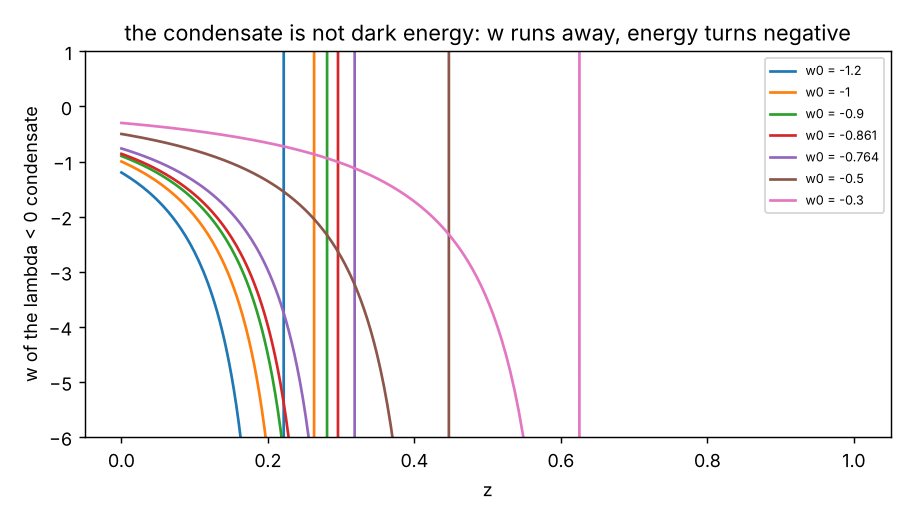
\includegraphics{figures/fig_analysis_condensate.png}
\caption{The equation of state of the \(\lambda < 0\) condensate for
several present values \(w_{\mathrm{de},0}\): \(w_{\mathrm{de}}\) runs
away to \(-\infty\) where the energy density crosses zero. The labels
are in the plain-text notation of the plotting script: ``z'' is the
redshift \(z_{\mathrm{red}}\), ``w'' is \(w_{\mathrm{de}}\) and ``w0''
is \(w_{\mathrm{de},0}\).}
\end{figure}

\hypertarget{the-vacuum-energy-and-the-tuning-open}{%
\subsubsection*{The vacuum energy and the tuning
(OPEN)}\label{the-vacuum-energy-and-the-tuning-open}}
\addcontentsline{toc}{subsubsection}{The vacuum energy and the tuning
(OPEN)}

A natural vacuum energy of the cell exceeds the observed dark-energy
density by 64 orders of magnitude:

\[ \rho_{\mathrm{vac}} = \frac{m_{\mathrm{KK}}^4}{16\pi^2} = 1.4\times10^{18}\ \text{GeV}^4,\qquad \frac{\rho_{\mathrm{vac}}}{\rho_{\mathrm{de}}} = 5.5\times10^{64}\qquad \big(\rho_{\mathrm{de}} = 2.5\times10^{-47}\ \text{GeV}^4\big) \]
\textbf{Symbols in this equation.}

\begin{itemize}
\tightlist
\item
  \(\rho_{\mathrm{vac}}\): A natural vacuum energy density of the cell,
  the fourth power of the Kaluza-Klein scale over \(16\pi^2\). Unit:
  GeV\(^4\). Value: \(1.4\times10^{18}\) GeV\(^4\). Status: ESTIMATE.
\item
  \(m^{\mathrm{KK}}_n,\ m_{\mathrm{KK}}\): The mass of the \(n\)-th
  Kaluza-Klein graviton (and gauge) level,
  \(m^{\mathrm{KK}}_n = \tilde m_n/(fL)\);
  \(m_{\mathrm{KK}} = m^{\mathrm{KK}}_1\) is the Kaluza-Klein scale.
  Unit: GeV. Value: \(m_{\mathrm{KK}} = 121.32\) TeV. Status: DERIVED.
\item
  \(\pi\): The number pi, the ratio of the circumference of a circle to
  its diameter. Unit: dimensionless. Value: 3.141592654. Status:
  STANDARD.
\item
  \(\rho_{\mathrm{de}}\): The observed energy density of the dark energy
  today. Unit: GeV\(^4\). Value: \(2.5\times10^{-47}\) GeV\(^4\).
  Status: STANDARD.
\end{itemize}

In UM-2 the four-dimensional cosmological term is the residual of the
stabiliser balance in the reduction of the Lovelock action on the static
block:

\[
\begin{aligned}
&\mathcal{L}_{(1)} = \mathcal{L}^{(4)}_{(1)} + \mathcal{L}^{(\mathrm{int})}_{(1)},\qquad
 \mathcal{L}_{(2)} = \mathcal{L}^{(4)}_{(2)} + 2\mathcal{L}^{(4)}_{(1)}\mathcal{L}^{(\mathrm{int})}_{(1)}
 + \mathcal{L}^{(\mathrm{int})}_{(2)},\qquad
 \mathcal{L}_{(3)} = 3\mathcal{L}^{(4)}_{(2)}\mathcal{L}^{(\mathrm{int})}_{(1)} +
 3\mathcal{L}^{(4)}_{(1)}\mathcal{L}^{(\mathrm{int})}_{(2)},\\
&\mathcal{L}^{(4)}_{(1)} = R^{(4)},\qquad \mathcal{L}^{(4)}_{(3)} = 0,\qquad
 \mathcal{L}^{(\mathrm{int})}_{(1)} = -12H^2K,\qquad
 \mathcal{L}^{(\mathrm{int})}_{(2)} = 24H^4K^2,\qquad \mathcal{L}^{(\mathrm{int})}_{(3)} = 0,\\
&\sum_{p=1}^{3}\alpha_{(p)}\,\mathcal{L}_{(p)} - 2\Lambda - 2\kappa\rho_{\mathrm{stab}}
 = \mathcal{G}(K)\,R^{(4)} + \text{(topological)} - 2\mathcal{G}(K)\,\Lambda_4,\\
&\Lambda_4 = \frac{6H^2K\big(1 - 2w_{(2)}K\big) + \Lambda + \kappa\rho_{\mathrm{stab}}}{\mathcal{G}(K)}
\end{aligned} \tag{FE-48}
\] \textbf{Symbols in (FE-48).}

\begin{itemize}
\tightlist
\item
  \(\mathcal{L}_{(p)}\): The Lovelock density of order \(p\) of the
  metric (a scalar built from \(p\) Riemann tensors):
  \(\mathcal{L}_{(1)} = R\) (Einstein-Hilbert), \(\mathcal{L}_{(2)}\)
  the Gauss-Bonnet density, \(\mathcal{L}_{(3)}\) the cubic Lovelock
  density. Unit: 1/\(\mathrm{length}^{2p}\). Status: STANDARD.
\item
  \(\mathcal{L}^{(4)}_{(r)}\): The Lovelock density of order \(r\) of
  the four-dimensional metric \(g^{(4)}_{\mu\nu}\)
  (\(\mathcal{L}^{(4)}_{(1)} = R^{(4)}\); the order 2 is topological and
  the order 3 vanishes in four dimensions). Unit:
  1/\(\mathrm{length}^{2r}\). Status: STANDARD.
\item
  \(\mathcal{L}^{(\mathrm{int})}_{(r)}\): The Lovelock density of order
  \(r\) of the static block (a four-dimensional space of constant
  curvature \(-H^2K\)): 1, \(-12H^2K\), \(24H^4K^2\), 0 for
  \(r = 0, 1, 2, 3\). Unit: 1/\(\mathrm{length}^{2r}\). Status: DERIVED.
\item
  \(R^{(4)}\): The Ricci scalar of the four-dimensional metric
  \(g^{(4)}_{\mu\nu}\). Unit: 1/\(\mathrm{length}^{2}\). Status:
  STANDARD.
\item
  \(H\): The author's constant (an inverse length) that fixes the period
  \(\pi/(6H)\) of \(x_0\), the Lovelock couplings, the cosmological
  constant \(\Lambda = -10H^2\) and the mass parameter \(m_\Psi = H\).
  Unit: GeV (1/length). Value: 14.296 TeV (from the fit of
  \(m_{\mathrm{W}}\) and \(\rho_{\mathrm{EW},0}\)). Status: AUTHOR.
\item
  \(K\): The block variable, \(K = 1/f^2\). Unit: dimensionless. Status:
  DERIVED.
\item
  \(p\): The Lovelock order \(p = 1, 2, 3\) (Einstein, Gauss-Bonnet,
  cubic). Status: STANDARD.
\item
  \(\alpha_{(p)}\): The Lovelock coupling of order \(p\),
  \(\alpha_{(p)} = w_{(p)}H^{2-2p}\) (\(\alpha_{(1)} = 1\)). Unit:
  \(\mathrm{GeV}^{2-2p}\). Status: AUTHOR.
\item
  \(\Lambda\): The eight-dimensional cosmological constant,
  \(\Lambda = -10H^2\). Unit: \(\mathrm{GeV}^{2}\). Value: \(-10H^2\).
  Status: AUTHOR.
\item
  \(\kappa\): The eight-dimensional gravitational coupling,
  \(\kappa = 8\pi G_8\). Unit: \(\mathrm{GeV}^{-6}\). Value:
  \(\kappa/V_\perp = 8\pi G_{\mathrm{N}}\mathcal{G}(K_*) = 2.328\times10^{-36}\)
  GeV\(^{-2}\). Status: AUTHOR.
\item
  \(\rho_{\mathrm{stab}}\): The energy density of the block stabiliser,
  a function of the block scale,
  \(\rho_{\mathrm{stab}} \propto f^{-8}\); its value at the static block
  is \(\rho_{\mathrm{stab}}(f_*)\). Unit: \(\mathrm{GeV}^{8}\). Value:
  \(\kappa\rho_{\mathrm{stab}}(f_*) = (26 + 4\sqrt{51})H^2 = 54.566\,H^2\).
  Status: ASSUMED.
\item
  \(\mathcal{G}(K)\): The coefficient of the four-dimensional
  Einstein-Hilbert term on a static block,
  \(\mathcal{G}(K) = 1 - 24w_{(2)}K + 72w_{(3)}K^2 = (K^2 - 12K + 16)/16\);
  four-dimensional gravity is attractive for \(\mathcal{G} > 0\). Unit:
  dimensionless. Value:
  \(\mathcal{G}(K_*) = 20/3 + \sqrt{51} = 13.8081\). Status: DERIVED.
\item
  \(\Lambda_4\): The four-dimensional cosmological constant of the
  effective theory on the block,
  \(\Lambda_4 = [6H^2K(1 - 2w_{(2)}K) + \Lambda + \kappa\rho_{\mathrm{stab}}]/\mathcal{G}(K)\);
  zero at the static point, the observed dark energy a tuned residual.
  Unit: \(\mathrm{GeV}^{2}\). Value: 0 at the static point; observed
  \(\Lambda_4/H^2 \sim 10^{-92}\). Status: DERIVED.
\item
  \(w_{(p)}\): The author's Lovelock weights, \(w_{(1)} = 1\),
  \(w_{(2)} = 1/32\), \(w_{(3)} = 1/1152\). Unit: dimensionless. Value:
  \((1, 1/32, 1/1152)\). Status: AUTHOR.
\end{itemize}

zero at the static point by construction. The observed dark energy needs

\[ \frac{\Lambda_4}{H^2} \sim \Big(\frac{\mathcal{H}_0}{H}\Big)^2 = 1.0\times10^{-92}: \]
\textbf{Symbols in this equation.}

\begin{itemize}
\tightlist
\item
  \(\Lambda_4\): The four-dimensional cosmological constant of the
  effective theory on the block,
  \(\Lambda_4 = [6H^2K(1 - 2w_{(2)}K) + \Lambda + \kappa\rho_{\mathrm{stab}}]/\mathcal{G}(K)\);
  zero at the static point, the observed dark energy a tuned residual.
  Unit: \(\mathrm{GeV}^{2}\). Value: 0 at the static point; observed
  \(\Lambda_4/H^2 \sim 10^{-92}\). Status: DERIVED.
\item
  \(H\): The author's constant (an inverse length) that fixes the period
  \(\pi/(6H)\) of \(x_0\), the Lovelock couplings, the cosmological
  constant \(\Lambda = -10H^2\) and the mass parameter \(m_\Psi = H\).
  Unit: GeV (1/length). Value: 14.296 TeV (from the fit of
  \(m_{\mathrm{W}}\) and \(\rho_{\mathrm{EW},0}\)). Status: AUTHOR.
\item
  \(\mathcal{H}_0\): The Hubble rate today (the Hubble constant). Unit:
  GeV (km/s/Mpc). Value: 67.38 km/s/Mpc. Status: DERIVED.
\end{itemize}

the cosmological-constant problem, unsolved (OPEN). A slowly deflating
block cannot provide a dynamical dark energy instead, because it would
make \(\alpha_{\mathrm{em}}\), \(G_{\mathrm{N}}\) and the masses drift
(\(\lvert\mathcal{H}_f\rvert < 3.6\times10^{-8}\,\mathcal{H}_0\),
section A.8), the neutrino oscillation lengths most of all.

\hypertarget{assessment-of-the-association-with-dark-energy}{%
\subsubsection*{Assessment of the association with dark
energy}\label{assessment-of-the-association-with-dark-energy}}
\addcontentsline{toc}{subsubsection}{Assessment of the association with
dark energy}

The association of dirac16complex with dark energy is not supported in
UM-2: its positive-energy states are matter or radiation, its only
accelerating configuration is unstable and reaches a negative energy
density at \(z_{\mathrm{red}} \approx 0.2\) to \(0.6\), and the measured
\((w_{\mathrm{de},0}, w_{\mathrm{de},a})\) are not reproduced. The dark
energy of UM-2 is the tuned four-dimensional cosmological term
\(\Lambda_4\).

\hypertarget{status-labels-conditions-open-problems-and-conflicts}{%
\section*{Status labels, conditions, open problems and
conflicts}\label{status-labels-conditions-open-problems-and-conflicts}}
\addcontentsline{toc}{section}{Status labels, conditions, open problems
and conflicts}

\begin{itemize}
\tightlist
\item
  \textbf{AUTHOR} (the author's input): the coordinates and the periodic
  hidden direction with the period \(\pi/(6H)\); the order-0 metric; the
  Lovelock weights and \(\Lambda = -10H^2\); the Clifford algebra and
  the two halves of dirac16complex; the order that every non-massless
  particle receive its mass from its \(x_0\) dependence, with the
  uncertainty relation as the reason, except the graviton, the photon
  and perhaps the quanta of dirac16complex.
\item
  \textbf{RECORD}: the dirac16complex Lagrangian and the Kohn-Sham
  functional of its self-interaction.
\item
  \textbf{DERIVED} (computed and verified): every mass as an \(x_0\)
  eigenvalue; the exact decompositions of the eigenvalues; the
  uncertainty relation on the cell and the lower bound
  \((1 - \varrho_\xi(-1))\,m_{\mathrm{Heis}}\), never below \(11.05\)
  TeV; the three classes of states; the zero-mode origin of the light
  masses and their hierarchy; the absence of tree-level flavour-changing
  neutral currents; the block sensitivities and the bounds on a
  deflation today; the candidate and its stability; the failure of I12
  alone and the relic with I13; the detection rates; the bound on the
  self-interaction; the freeze-in of the fold bands; the non-negative
  equation of state of every Kohn-Sham state; the runaway of the
  condensate.
\item
  \textbf{ASSUMED} (conditions on which the conclusions rest): the
  stabiliser and its \(f^{-8}\) law; the good sector; the regular tip at
  \(HL = 3\); \(m_\Psi = H\); the tip sigma field, the tip matrices and
  the boundary assignments of the Standard-Model fields of three
  generations; the lightest neutrino mass \(m_1 = 1\) meV and the normal
  ordering; the benchmark strengths of I11 and I12, the bound
  \(G_\lambda \le 2.3\times10^{-15}\) GeV\(^{-2}\) on the
  self-interaction and the highest temperature \(T_{\mathrm{max}} = 10\)
  TeV (the strength of I13 follows from the relic abundance).
\item
  \textbf{INVENTED}: the portals I11, I12 and I13; the tip sigma field
  without a radial mode (no Higgs particle) and the fermion boundary
  conditions.
\item
  \textbf{ESTIMATE}: the radion decay and the reheating temperature; the
  direct-detection limit extrapolated to 44 TeV; the cross-section of
  the self-interaction channel (Fierz coefficients not computed); the
  elastic rate of the right-handed neutrinos; the effect of the
  order-\(\alpha\) plasma pressure on the relic (about 2.7 \% in
  \(\Omega_{\mathrm{DM}}h_{100}^2\), 1.4 \% in \(G_{\mathrm{A}}\)); the
  one-loop sensitivity of the nucleon mass.
\item
  \textbf{OPEN}: the origin of the stabiliser; the extra-time modes; the
  closed time-like curves implied by compact extra times; the radion
  moduli problem; the block-shape mode driven by \(p_0 - p_5\) (about 4
  times the kept hidden pressure for non-relativistic dark matter, but
  absolutely suppressed); the microscopic origin of the portals (I12
  alone could give the relic only as a strongly coupled \(^3P_0\)
  channel; I13 gives it, and its contact form needs a mediator above
  about 30 TeV); the gravitational production of the fold bands; the
  origin of the tip matrices (the mixing angles); Dirac or Majorana
  neutrinos (the mechanism favours Dirac); the cosmological-constant
  problem.
\item
  \textbf{Conflicts with data inherent in the order}: no Higgs boson
  (one is observed), and perturbative unitarity of \(W^+W^-\) scattering
  lost near 1.2 TeV. (The one-generation conflict of version 1, a \(Z\)
  width of \(1.23\) GeV, is removed: three generations give \(2.485\)
  GeV against the measured \(2.4955\) GeV; the two values of the weak
  angle, on shell in the \(x_0\) problem and \(\overline{\mathrm{MS}}\)
  in the widths, move the width by 0.83 \%, within the loop corrections
  that UM-2 does not compute.)
\end{itemize}

\hypertarget{closing-assessment}{%
\section*{Closing assessment}\label{closing-assessment}}
\addcontentsline{toc}{section}{Closing assessment}

\textbf{The \(x_0\) mass mechanism.} The author's requirement is
realised exactly in UM-2: every wave function depends on \(x_0\)
periodically with the period \(\pi/(6H)\), every four-dimensional mass
is an eigenvalue of the \(x_0\) operator of its field, and the massless
particles (the photon, the gluons, the graviton and the fold bands of
dirac16complex) are exactly the zero modes that symmetry protects, which
are also the exceptions the author names. The author's physical reason,
the uncertainty relation, holds as a theorem on the cell (with a tip
term) and is quantitative for the heavy states: the Kaluza-Klein and odd
excitations and the dark matter lie above the estimate
\(m_{\mathrm{Heis}}\), by factors 2.3 to 7.5, and the dark-matter mass
is 90 \% hidden momentum. It fails for every light particle: the bound
it sets on the hidden kinetic energy of a localised state is at least
\(11.05\) TeV, while the observed masses of \(W^\pm\), \(Z\) and all
twelve fermions lie \(3\times10^{-3}\) to \(10^{-17}\) below their
estimates. Those masses come from exact zero modes, whose hidden kinetic
energy is cancelled exactly, mixed at the tip of the cell, where the
electroweak symmetry is broken; the exponential tip densities turn
order-one bulk masses into the fourteen orders of magnitude of the
fermion masses, a sharper localisation giving a lighter particle. The
mixing matrices are inputs (tip matrices), and the extra times are
irrelevant today because the block is small and frozen, not because it
keeps deflating.

\textbf{dirac16complex as dark matter.} Supported, conditionally. The
heavy odd quanta of the two halves, two degenerate Dirac fermions of
44.35 TeV, are cold, neutral and stable in the good sector with an exact
fold parity. They obtain the observed relic density only through the
INVENTED s-wave portal I13 to the baryon-number current
(\(G_{\mathrm{A}} = 1.28\times10^{-9}\) GeV\(^{-2}\), about 1 \% physics
accuracy), since the gauge-kinetic portal alone would violate
partial-wave unitarity; the candidate predicts a spin-independent
cross-section on xenon at 0.16 of the present LZ limit and is therefore
falsifiable by the next generation of xenon detectors. The field as a
whole is not dark matter: its massless fold bands are a trace of dark
radiation (\(\Delta N_{\mathrm{eff}} = 0.001\)), kept out of equilibrium
by the weak portal I11 and a bounded self-interaction.

\textbf{dirac16complex as dark energy.} Not supported. No
positive-energy state of the field has a negative equation of state, the
only accelerating configuration (a negative-coupling condensate) runs
away to a negative energy density at a redshift of 0.2 to 0.6 and does
not reproduce the measured \((w_{\mathrm{de},0}, w_{\mathrm{de},a})\),
and the dark energy of UM-2 is the four-dimensional cosmological term
\(\Lambda_4\) of the stabilised block, tuned to \(10^{-92}H^2\): the
cosmological-constant problem remains open.

\end{document}
